
% ----------------------------------------------------------------------
%                   LATEX TEMPLATE FOR PhD THESIS
% ----------------------------------------------------------------------

% based on Harish Bhanderi's PhD/MPhil template, then Uni Cambridge
% http://www-h.eng.cam.ac.uk/help/tpl/textprocessing/ThesisStyle/
% corrected and extended in 2007 by Jakob Suckale, then MPI-CBG PhD programme
% and made available through OpenWetWare.org - the free biology wiki


%: Style file for Latex
% Most style definitions are in the external file PhDthesisPSnPDF.
% In this template package, it can be found in ./Latex/Classes/
\documentclass[twoside,12pt]{Latex/Classes/PhDthesisPSnPDF}

\makeatletter
        \setlength{\@fptop}{0pt}
\makeatother


%: Macro file for Latex
% Macros help you summarise frequently repeated Latex commands.
% Here, they are placed in an external file /Latex/Macros/MacroFile1.tex
% An macro that you may use frequently is the figuremacro (see introduction.tex)
% This file contains macros that can be called up from connected TeX files
% It helps to summarise repeated code, e.g. figure insertion (see below).

% insert a centered figure with caption and description
% parameters 1:filename, 2:title, 3:description and label
\newcommand{\figuremacro}[3]{
	\begin{figure}[htbp]
		\centering
		\includegraphics[width=1\textwidth]{#1}
		\caption[#2]{\textbf{#2} - #3}
		\label{#1}
	\end{figure}
}

% insert a centered figure with caption and description AND WIDTH
% parameters 1:filename, 2:title, 3:description and label, 4: textwidth
% textwidth 1 means as text, 0.5 means half the width of the text
\newcommand{\figuremacroW}[4]{
	\begin{figure}[htbp]
		\centering
		\includegraphics[width=#4\textwidth]{#1}
		\caption[#2]{\textbf{#2} - #3}
		\label{#1}
	\end{figure}
}

% inserts a figure with wrapped around text; only suitable for NARROW figs
% o is for outside on a double paged document; others: l, r, i(inside)
% text and figure will each be half of the document width
% note: long captions often crash with adjacent content; take care
% in general: above 2 macro produce more reliable layout
\newcommand{\figuremacroN}[3]{
	\begin{wrapfigure}{o}{0.5\textwidth}
		\centering
		\includegraphics[width=0.48\textwidth]{#1}
		\caption[#2]{{\small\textbf{#2} - #3}}
		\label{#1}
	\end{wrapfigure}
}

% predefined commands by Harish
\newcommand{\PdfPsText}[2]{
  \ifpdf
     #1
  \else
     #2
  \fi
}

\newcommand{\IncludeGraphicsH}[3]{
  \PdfPsText{\includegraphics[height=#2]{#1}}{\includegraphics[bb = #3, height=#2]{#1}}
}

\newcommand{\IncludeGraphicsW}[3]{
  \PdfPsText{\includegraphics[width=#2]{#1}}{\includegraphics[bb = #3, width=#2]{#1}}
}

\newcommand{\InsertFig}[3]{
  \begin{figure}[!htbp]
    \begin{center}
      \leavevmode
      #1
      \caption{#2}
      \label{#3}
    \end{center}
  \end{figure}
}


%%% Local Variables: 
%%% mode: latex
%%% TeX-master: "~/Documents/LaTeX/CUEDThesisPSnPDF/thesis"
%%% End: 

\usepackage[table]{xcolor}
%% The amssymb package provides various useful mathematical symbols
\usepackage{amssymb}

%% The amsthm package provides extended theorem environments
\usepackage{amsthm}

%% amsmath for math environment
\usepackage{amsmath}

\DeclareMathOperator*{\argmin}{arg\,min}
\DeclareMathOperator*{\argmax}{arg\,max}
\DeclareMathOperator*{\sign}{sign}
\DeclareMathOperator*{\infspie}{inf}


% to break equation
%\usepackage{mathpazo}
%\usepackage{mathptmx}
%\usepackage[mathpazo]{flexisym}
%\usepackage{breqn}

%% For clever reference
%\usepackage{cleveref}

%% color package
\usepackage{color}

%% figure package
\usepackage{epsf,graphicx}
\usepackage{epstopdf}
\usepackage{subfigure}	
\usepackage{transparent}

%% New environment to have some indent inside enumerate environment
\usepackage{enumitem}

%% To create acronym for proper glossary
\usepackage{acro}

%% To number the line in the article
\usepackage{lineno}

%% Environment to include table with notes
\usepackage{array}
\usepackage{threeparttable}
\usepackage{booktabs}
\usepackage{multirow}
\usepackage{siunitx}

%% In order to change size of margin
\usepackage{geometry}
\usepackage{changepage}
\usepackage{lscape}
%% Colorpackage for table
\usepackage{colortbl}
\usepackage{tabularx}
\usepackage{arydshln}

%% To use URL referencing
\usepackage{url}
%\usepackage[hidelinks]{hyperref}

%% In order to draw some graphs
\usepackage{tikz,xifthen}
\usepackage{tikz-qtree}
\usetikzlibrary{decorations.pathmorphing} % noisy shapes
\usetikzlibrary{fit}					% fitting shapes to coordinates
\usetikzlibrary{backgrounds}	% drawing the background after the foreground
\usetikzlibrary{shapes,arrows,shadows}
\usetikzlibrary{calc,decorations.pathreplacing,decorations.markings,positioning}
\usetikzlibrary{snakes,decorations.text,shapes,patterns}
%\usepackage{scalefnt,lmodern,booktabs}

%% Paxkage for cross and tick symbols
\usepackage{pifont}
\newcommand{\cmark}{\large \color{green!60!black!80}\ding{51}}
\newcommand{\mmark}{\large {\color{green!60!black!80}\ding{51}}$^{!}$}
\newcommand{\xmark}{\large \color{red!60!black!80}\ding{55}}
\newcommand{\cmarksmall}{\color{green!60!black!80}\ding{51}}
\newcommand{\mmarksmall}{{\color{green!60!black!80}\ding{51}}$^{!}$}
\newcommand{\xmarksmall}{\color{red!60!black!80}\ding{55}}
\newcommand{\Conv}{\mathop{\scalebox{1.5}{\raisebox{-0.2ex}{$\ast$}}}}%

\definecolor{autoGuided}{rgb}{ 0.3765    0.7294    0.9412}
\newcommand{\autoGuidedColor}{(light-Blue)}
\definecolor{fullyAuto}{rgb}{ 0.0941    0.3843    0.6627}
\newcommand{\fullyAutoColor}{(dark-blue)}
\definecolor{semiAuto}{rgb}{ 0.0784    0.5059    0.1686}
\newcommand{\semiAutoColor}{(light-green)}
\definecolor{fullyGuided}{rgb}{ 0.4275    0.6902    0.3176}
\newcommand{\fullyGuidedColor}{(dark-green)}

\DeclareSIUnit\ppm{ppm}
%\acrodef{cap}[CaP]{prostate cancer}
\DeclareAcronym{cap}{
short = CaP,
long = prostate cancer
}
%\acrodef{cade}[CADe]{computer-aided detection}
\DeclareAcronym{cade}{
short = CADe,
long = computer-aided detection
}
%\acrodef{cadx}[CADx]{computer-aided diagnosis}
\DeclareAcronym{cadx}{
short = CADx,
long = computer-aided diagnosis
}
\DeclareAcronym{lm}{
short = LM, 
long = Leung-Malik set
}
%\acrodef{us}[US]{ultrasound}
\DeclareAcronym{us}{
short = US,
long = ultrasound
}
%\acrodef{ct}[CT]{computer tomography}
\DeclareAcronym{ct}{
short = CT,
long = computer tomography
}
%\acrodef{cad}[CAD]{computer-aided detection and diagnosis}
\DeclareAcronym{cad}{
short = CAD,
long = computer-aided detection and diangosis
}
%\acrodef{mri}[MRI]{magnetic resonance imaging}
\DeclareAcronym{mri}{
short = MRI,
long = magnetic resonance imaging
}
%\acrodef{nmr}[NMR]{nuclear magnetic resonance}
\DeclareAcronym{nmr}{
short = NMR,
long = nuclear magnetic resonance
}

\DeclareAcronym{omp}{
  short = OMP,
  long =  Orthogonal Matching Pursuit 
}
\DeclareAcronym{adb}{
  short = AdB, 
  long = AdaBoost
}
\DeclareAcronym{gb}{
  short = GB, 
  long = Gradient Boosting
}

\DeclareAcronym{mp}{
  short = MP,
  long =  Matching Pursuit 
}
%\acrodef{t2w}[T$_2$-W]{T$_2$ Weighted}
\DeclareAcronym{t2w}{
short = T$_2$-W,
long = T$_2$ Weighted
}
%\acrodef{dce}[DCE]{dynamic contrast-enhanced}
\DeclareAcronym{dce}{
short = DCE,
long = dynamic contrast-enhanced
}
%\acrodef{dw}[DW]{diffusion weighted}
\DeclareAcronym{dw}{
short = DW,
long = diffusion weighted
}
%\acrodef{mrsi}[MRSI]{magnetic resonance spectroscopy imaging}
\DeclareAcronym{mrsi}{
short = MRSI,
long = magnetic resonance spectroscopy imaging
}
%\acrodef{bph}[BPH]{benign prostatic hyperplasia}
\DeclareAcronym{bph}{
short = BPH,
long = benign prostatic hyperplasia
}
%\acrodef{pz}[PZ]{peripheral zone}
\DeclareAcronym{pz}{
short = PZ,
long = peripheral zone
}
%\acrodef{cz}[CZ]{central zone}

\DeclareAcronym{mpmri}{
short = mp-MRI,
long = multiparametric \ac{mri}
}
\DeclareAcronym{cz}{
short = CZ,
long = central zone
}
%\acrodef{tz}[TZ]{transitional zone}
\DeclareAcronym{tz}{
short = TZ,
long = transitional zone
}
%\acrodef{cg}[CG]{central gland}
\DeclareAcronym{cg}{
short = CG,
long = central gland
}
%\acrodef{psa}[PSA]{prostate-specific antigen}
\DeclareAcronym{psa}{
short = PSA,
long = prostate-specific antigen
}
%\acrodef{trus}[TRUS]{transrectal ultrasound}
\DeclareAcronym{trus}{
short = TRUS,
long = transrectal ultrasound
}
%\acrodef{tr}[TR]{repetition time}
\DeclareAcronym{tr}{
short = TR,
long = repetition time
}
%\acrodef{te}[TE]{echo time}
\DeclareAcronym{te}{
short = TE,
long = echo time
}
%\acrodef{si}[SI]{signal intensity}
\DeclareAcronym{si}{
short = SI,
long = signal intensity
}
%\acrodef{ees}[EES]{extravascular-extracellular space}
\DeclareAcronym{ees}{
short = EES,
long = extravascular-extracellular space
}
%\acrodef{t1w}[T$_1$-W]{T$_1$ Weighted}
\DeclareAcronym{t1w}{
short = T$_1$-W,
long = T$_1$ Weighted
}
%\acrodef{fse}[FSE]{Fast Spin-Echo}
\DeclareAcronym{fse}{
short = FSE,
long = Fast Spin-Echo
}
%\acrodef{adc}[ADC]{Apparent Diffusion Coeffient}
\DeclareAcronym{adc}{
short = ADC,
long = apparent diffusion coefficient
}
%\acrodef{roi}[ROI]{region of interest}
\DeclareAcronym{roi}{
short = ROI,
long = region of interest
}
%\acrodef{cse}[CSE]{chemical shift effect}
\DeclareAcronym{cse}{
short = CSE,
long = chemical shift effect
}
%\acrodef{snr}[SNR]{signal-to-noise}
\DeclareAcronym{snr}{
short = SNR,
long = signal-to-noise
}
\DeclareAcronym{se}{
short = SE, 
long = sensitivity
}
\DeclareAcronym{sp}{
short = SP, 
long = Specificity
}
%\acrodef{gs}[GS]{Gleason score}
\DeclareAcronym{gs}{
short = GS,
long = Gleason score
}
%\acrodef{ersspc}[ERSSPC]{European Randomized Study of Screening for Prostate Cancer}
\DeclareAcronym{ersspc}{
short = ERSSPC,
long = European randomized study of screening for prostate cancer
}
%\acrodef{plco}[PLCO]{Prostate, Lung, Colorectal and Ovarian}
\DeclareAcronym{plco}{
short = PLCO,
long = prostate lung colorectal and ovarian
}
%\acrodef{fig}[Fig.]{figure}
\DeclareAcronym{fig}{
short = Fig.,
long = figure
}
\DeclareAcronym{tab}{
short = Table,
long = table
}
\DeclareAcronym{eq}{
short = Eq.,
long = equation
}
\DeclareAcronym{sec}{
short = Sect.,
long = section
}
\DeclareAcronym{chp}{
short = Chap.,
long = Chapter
}

\DeclareAcronym{fov}{
short = FOV,
long = field of view
}
\DeclareAcronym{dwt}{
short = DWT,
long = discrete wavelet transform
}
\DeclareAcronym{dwst}{
short = DWST,
long = discrete wavelet squared transform
}
\DeclareAcronym{map}{
short = MAP,
long = maximum \textit{a posteriori}
}
\DeclareAcronym{ml}{
short = ML,
long = maximum likelihood
}
\DeclareAcronym{mle}{
short = MLE,
long = maximum likelihood estimation
}
\DeclareAcronym{mrf}{
short = MRF,
long = Markov random field
}
\DeclareAcronym{itk}{
short = ITK,
long = Insight Segmentation and Registration Toolkit
}
\DeclareAcronym{es}{
short = ES,
long = Evolution Strategy
}
\DeclareAcronym{scf}{
short = SCF,
long = sparse coded features
}
\DeclareAcronym{bow}{
short = BoW,
long = Bag of Words
}
\DeclareAcronym{pdf}{
short = PDF,
long = probability density function
}
\DeclareAcronym{gscale}{
short = \textit{g}-scale,
long = generalized scale
}
\DeclareAcronym{aif}{
short = AIF,
long = arterial input function
}
\DeclareAcronym{svd}{
short = SVD,
long = singular value decomposition
}
\DeclareAcronym{mse}{
short = MSE,
long = mean squared error
}
\DeclareAcronym{mi}{
short = MI,
long = mutual information
}
\DeclareAcronym{mantra}{
short = MANTRA,
long = multi-attribute non-initializing texture reconstruction based active shape model
}
\DeclareAcronym{asm}{
short = ASM,
long = active shape model
}
\DeclareAcronym{pca}{
short = PCA,
long = principal components analysis
}
\DeclareAcronym{weritas}{
short = WERITAS,
long = weighted ensemble of regional image textures for active shape model segmentation
}
\DeclareAcronym{staple}{
short = STAPLE,
long = simultaneous truth and performance level estimation
}
\DeclareAcronym{lda}{
short = LDA,
long = linear discriminant analysis
}
\DeclareAcronym{lbp}{
short = LBP,
long = local binary pattern
}
\DeclareAcronym{tps}{
short = TPS,
long = thin plate spline
}
\DeclareAcronym{acm}{
short = ACM,
long = active contour model
}
\DeclareAcronym{cmi}{
short = CMI,
long = combined mutual information
}
\DeclareAcronym{svm}{
short = SVM,
long = support vector machines
}
\DeclareAcronym{rvm}{
short = RVM,
long = relevant vector machine
}
\DeclareAcronym{rbf}{
short = RBF,
long = radial basis function
}
\DeclareAcronym{knn}{
short = $k$-NN,
long = $k$-neareast neighbour
}
\DeclareAcronym{nn}{
short = NN,
long = neareast neighbour
}
\DeclareAcronym{dct}{
short = DCT,
long = discrete cosine transform
}
\DeclareAcronym{hog}{
short = HOG,
long = histogram of oriented gradient
}
\DeclareAcronym{dft}{
short = DFT,
long = discrete fourier transform
}
\DeclareAcronym{us1}{
short = US,
long = under-sampling
}
\DeclareAcronym{os}{
short = OS,
long = over-sampling
}
\DeclareAcronym{ros}{
short = ROS,
long = random-over-sampling
}
\DeclareAcronym{rus}{
short = RUS,
long = random-under-sampling
}
\DeclareAcronym{nm}{
short = NM,
long = nearmiss
}
\DeclareAcronym{nm3}{
short = NM-3,
long = nearmiss-3
}
\DeclareAcronym{nm2}{
short = NM-2,
long = nearmiss-2
}
\DeclareAcronym{nm1}{
short = NM-1,
long = nearmiss-1
}
\DeclareAcronym{iht}{
short = IHT,
long = instance-hardness-threshold
}
\DeclareAcronym{smote}{
short = SMOTE,
long = synthetic minority over-sampling techniques
}
\DeclareAcronym{smoteb1}{
short = SMOTE-b1,
long = SMOTE-borderline1
}
\DeclareAcronym{smoteb2}{
short = SMOTE-b2,
long = SMOTE-borderline2
}
\DeclareAcronym{mrmr}{
short = mRMR,
long = minimum redundancy maximum relevance
}
\DeclareAcronym{lle}{
short = LLE,
long = locally linear embedding
}
\DeclareAcronym{ica}{
short = ICA,
long = independent components analysis
}
\DeclareAcronym{qda}{
short = QDA,
long = quadratic discriminant analysis
}
\DeclareAcronym{id3}{
short = ID3,
long = iterative dichotomiser 3
}
\DeclareAcronym{cart}{
short = CART,
long = classification and regression tree
}
\DeclareAcronym{bagging}{
short = bagging,
long = bootsrap aggregating
}
\DeclareAcronym{loo}{
short = LOOCV,
long = leave-one-out cross-validation
}
\DeclareAcronym{lopo}{
short = LOPO CV,
long = leave-one-patient-out cross-validation
}

\DeclareAcronym{kcv}{
short = $k$-CV,
long = $k$-fold cross-validation
}
\DeclareAcronym{roc}{
short = ROC,
long = receiver operating characteristic
}
\DeclareAcronym{froc}{
short = FROC,
long = free-response receiver operating characteristic
}
\DeclareAcronym{auc}{
short = AUC,
long = area under the curve
}
\DeclareAcronym{rmse}{
short = RMSD,
long = root-mean-square deviation
}
\DeclareAcronym{rms}{
  short = RMS,
  long = root mean square
}
\DeclareAcronym{srsf}{
  short = SRSF,
  long =  square-root slope function
}
\DeclareAcronym{pun}{
short = PUN,
long = phenomenological universalities
}
\DeclareAcronym{etl}{
short = ETL,
long = echo train ength
}

\DeclareAcronym{rf}{
short = RF,
long = random forest
}
\DeclareAcronym{dna}{
short = DNA,
long = deoxyribonucleic acid
}

\DeclareAcronym{glcm}{
short = GLCM,
long = gray-level co-occurence matrix
}

\DeclareAcronym{pd}{
short = PD,
long = proton density
}



%: ----------------------------------------------------------------------
%:                  TITLE PAGE: name, degree,..
% ----------------------------------------------------------------------
% below is to generate the title page with crest and author name

%if output to PDF then put the following in PDF header
\ifpdf  
    \pdfinfo { /Title  (Computer Aided Diagnosis system for prostatic biopsy guidance and follow-up fusing multi-modal imaging)
               /Creator (TeX)
               /Producer (pdfTeX)
               /Author (Guillaume Lemaitre g.lemaitre58@gmail.com)
               /CreationDate (D:201610151200ss)  %format D:YYYYMMDDhhmmss
               /ModDate (D:201610151200ss)
               /Subject (PhD Dissertation of Guillaume Lemaitre)
               /Keywords (CAD, mp-MRI, spectroscopy, MRI) }
    \pdfcatalog { /PageMode (/UseOutlines)
                  /OpenAction (fitbh)  }
\fi


\title{Computer Aided Diagnosis system for prostatic biopsy guidance and follow-up fusing multi-modal imaging}



% ----------------------------------------------------------------------
% The section below defines www links/email for author and institutions
% They will appear on the title page of the PDF and can be clicked
\ifpdf
  \author{\href{mailto:guillaume.lemaitre@udg.edu}{Guillaume Lema\^itre}}
%  \cityofbirth{born in XYZ} % uncomment this if your university requires this
%  % If city of birth is required, also uncomment 2 sections in PhDthesisPSnPDF
%  % Just search for the "city" and you'll find them.
  % The crest is a graphics file of the logo of your research institution.
  % Place it in ./0_frontmatter/figures and specify the width

%% First university
  \firstlab{\href{http://le2i.cnrs.fr/}{LE2I}}
  \firstlogolab{
\includegraphics[width=2cm]{logos/logole2i.eps}}
  \firstuni{\href{http://www.u-bourgogne.fr/}{Universit\'e de Bourgogne}}
  \firstlogouni{
\includegraphics[width=2cm]{logos/logo-ub-no-bg.pdf}}

  
%% Second university
  \secondlab{\href{http://vicorob.udg.es/}{ViCOROB}}
  \secondlogolab{
\includegraphics[width=2cm]{logos/vicorobLogo1.png}}

  \seconduni{\href{https://www.udg.edu/}{Universitat de Girona}}
  \secondlogouni{
\includegraphics[scale =0.5]{logos/UdG_dues_linies_centrat_blau.png}}
  
  \supervisora{Jordi Freixenet Bosch (ViCOROB - UdG)}
  \supervisorb{Fabrice M\'eriaudeau (CISIR - UTP)}
  \supervisorc{Robert Mar\'i Marly (ViCOROB - UdG)}
  \supervisord{Paul Michael Walker (LE2I - UBFC)}
  
% If you are not creating a PDF then use the following. The default is PDF.
\else
  \author{Guillaume Lema\^itre}
%  \cityofbirth{born in XYZ}
%% First university
  \firstlab{\href{http://le2i.cnrs.fr/}{LE2I}}
  \firstlogolab{
\includegraphics[width=2cm]{logos/logole2i.eps}}
  \firstuni{\href{http://www.u-bourgogne.fr/}{Universit\'e de Bourgogne}}
  \firstlogouni{
\includegraphics[width=2cm]{logos/logoubblue.eps}}
  
%% Second university
  \secondlab{\href{http://vicorob.udg.es/}{ViCOROB}}
  \secondlogolab{
\includegraphics[width=2cm]{logos/logovicorob.eps}}
  \seconduni{\href{https://www.udg.edu/}{Universitat de Girona}}
  \secondlogouni{
\includegraphics[width=2cm]{logos/logoudg.eps}}
  
  
  \supervisora{Fabrice M\'eriaudeau (CISIR - UTP)}
  \supervisorb{Robert Mar\'i Marly (ViCOROB - UdG)}
  \supervisorc{Jordi Freixenet Bosch (ViCOROB - UdG)}
  \supervisord{Paul Michael Walker (LE2I - UBFC)}
\fi

%\renewcommand{\submittedtext}{change the default text here if needed}
\degree{Philosophi\ae Doctor (PhD)}
\degreedate{November 2016}


% ----------------------------------------------------------------------
       
% turn of those nasty overfull and underfull hboxes
\hbadness=10000
\hfuzz=50pt


%: --------------------------------------------------------------
%:                  FRONT MATTER: dedications, abstract,..
% --------------------------------------------------------------

\begin{document}

%\language{english}

% sets line spacing
\renewcommand\baselinestretch{1.2}
\baselineskip=18pt plus1pt


%: ----------------------- generate cover page ------------------------

\maketitle  % command to print the title page with above variables


%: ----------------------- cover page back side ------------------------
% Your research institution may require reviewer names, etc.
% This cover back side is required by Dresden Med Fac; uncomment if needed.

\newpage
\vspace{10mm}
Reviewers:

\begin{itemize}
\item[] Su Ruan, Professor at Universit\'e de Rouen - LITIS
\item[] Reyer Zwiggelaar Ir, Professor at Aberystwyth Universtiy - Vision, Graphics, and Visualisation Group
\item[] Soumya Ghose, Research Associate at Case Western Reserve University
\end{itemize}

\vspace{20mm}
Day of the defense: December 2016

\vspace{20mm}
\hspace{70mm}Signature from head of PhD committee:



%: ----------------------- abstract ------------------------

% Your institution may have specific regulations if you need an abstract and where it is to be placed in the document. The default here is just after title.


% Thesis Abstract -----------------------------------------------------


%\begin{abstractslong}    %uncommenting this line, gives a different abstract heading
\begin{abstracts}        %this creates the heading for the abstract page
Prostate cancer (CaP) is the second most diagnosed cancer in men all over the world.
CaP growth is characterized by two main types of evolution: (i) the slow-growing tumours progress slowly and usually remain confined to the prostate gland; (ii) the fast-growing tumours metastasize from prostate gland to other organs, which might lead to incurable diseases.
Therefore, early diagnosis and risk assessment play major roles in patient treatment and follow-up.
In the last decades, new imaging techniques based on Magnetic Resonance Imaging (MRI) have been developed improving diagnosis.
In practise, diagnosis can be affected by multiple factors such as observer variability and visibility and complexity of the lesions.
In this regard, computer-aided detection and computer-aided diagnosis systems are being designed to help radiologists in their clinical practice.

Our research extensively analyzes the current state-of-the-art in the development of computer-aided diagnosis and detection systems for prostate cancer detection.
Currently, no computer-aided system using all available MRI modalities has been proposed and tested on a common dataset.
Therefore, we propose a new computer-aided system taking advantage of all MRI modalities (i.e., \acs{t2w}-\acs{mri}, \acs{dce}-\acs{mri}, DW-\acs{mri}, \acs{mrsi}).
Particular attention is paid to the normalization of the \acs{mri} modalities prior to develop our computer-aided system.
This system has been extensively tested on a dataset which has been made publicly available.
\end{abstracts}
%\end{abstractlongs}
%-------------------------------------------------------------------------

\begin{abstractCatalan}

El c\`ancer de pr\`ostata (CaP) \'es el segon c\`ancer m\'es diagnosticat en homes a tot el m\'on.
El creixement del CaP es caracteritza per dos tipus principals d'evoluci\'o: (i) els tumors de creixement lent que progressen lentament i en general romanen confinats en la gl\`andula de la pr\`ostata; (Ii) els tumors de creixement r\`apid que desenvolupen met\`astasi de la pr\`ostata a altres \`organs, el que podria conduir a malalties incurables.
Conseqüentment, el diagn\`ostic preco\c{c} i l'avaluaci\'o del risc exerceixen un paper important en el tractament del pacient i el seguiment.
En les \'ultimes dècades s'han desenvolupat noves t\'ecniques d'imatge basades en imatge de resson\'ancia magn\`etica (RM, o MRI de l'angl\`es) per millorar el diagnòstic.
A la pr\`actica, el diagn\`ostic pot ser afectat per diversos factors com ara la variabilitat de l'observador i la visibilitat i la complexitat de les lesions.
En aquest sentit, s'estan desenvolupant sistemes per a l'ajuda a la detecci\'o i diagn\`ostic per ordinador per ajudar els radiòlegs en la seva pràctica clínica.

La nostra recerca analitza \`ampliament l'estat de l'art en el desenvolupament de sistemes per a l'ajuda a la detecci\'o i diagn\`ostic per ordinador per a la detecci\'o del c\`ancer de pr\`ostata.
En l'actualitat, no hi ha cap sistema d'ajuda al diagn\`ostic que utilitzi totes les modalitats de MRI disponibles i que hagi estat avaluat en un conjunt de dades com\'u.
Per tant, proposem un nou sistema d'ajuda al diagn\`ostic per ordinador aprofitant totes les modalitats de resson\`ancia magn\`etica (\'es a dir \acs{t2w}-MRI, DCE-MRI, DW-MRI, MRSI).
Com a etapa pr\`evia al desenvolupament del sistema, es presta especial atenci\'o a la normalitzaci\'o de les modalitats de resson\`ancia magn\`etica.
El sistema desenvolupat ha estat avaluat extensivament en un conjunt de dades que s'han posat a disposició pública.
 
\end{abstractCatalan}

% ---------------------------------------------------------------------- 
\begin{abstractSpanish}

El c\`ancer de pr\'ostata (CaP) es el segundo c\`ancer m\'as diagnosticado en hombres en todo el mundo.
El crecimiento del CaP se caracteriza por dos tipos principales de evoluci\'on: (i) los tumores de crecimiento lento que progresan lentamente y por lo general permanecen confinados en la gl\'andula de la pr\'ostata; (ii) los tumores de crecimiento r\'apido que desarrollan met\'astasis de la pr\'ostata a otros \'organos, lo que podr\'ia conducir a enfermedades incurables.
Consecuentemente, el diagn\'ostico precoz y la evaluaci\'on del riesgo desempe\~nan un papel importante en el tratamiento del paciente y el seguimiento. En las \'ultimas d\'ecadas se han desarrollado  nuevas t\'ecnicas de imagen basadas en imagen de resonancia magn\'etica (RM, o MRI del ingl\'es) para mejorar el diagn\'ostico. En la pr\'actica, el diagn\'ostico puede ser afectado por varios factores tales como la variabilidad del observador y la visibilidad y la complejidad de las lesiones.
En este sentido, se est\'an desarrollando sistemas para la ayuda a la detecci\'on y diagnóstico por ordenador para ayudar a los radi\'ologos en su pr\'actica cl\'inica.

Nuestra investigaci\'on analiza ampliamente el estado del arte en el desarrollo de sistemas para la ayuda a la detecci\'on y diagn\'ostico por ordenador para la detecci\'on del c\`ancer de pr\'ostata.
En la actualidad, no existe ning\'un sistema de ayuda al diagn\'ostico que utilice todas las modalidades de MRI disponibles y que haya sido evaluado en un conjunto de datos com\'un.
Por lo tanto, proponemos un nuevo sistema de ayuda al diagn\'ostico por ordenador aprovechando todas las modalidades de resonancia magnética (es decir T2W-MRI, DCE-MRI, DW-MRI, MRSI).
Como etapa previa al desarrollo del sistema, se presta especial atenci\'on a la normalizaci\'on de las modalidades de resonancia magn\'etica.
El sistema desarrollado ha sido evaluado extensivamente en un conjunto de datos que se han puesto a disposici\'on p\'ublica.
 
\end{abstractSpanish}

%-------------------------------------------------------------------------
\begin{abstractFrench}

Le cancer de la prostate est le second type de cancer le plus diagnostiqu\'e au monde.
Il est caract\'eris\'e par deux evolutions distinctes : (i) les tumeurs \`a croissances lentes progressent lentement et restent g\'en\'eralement confin\'ees dans la glande prostatique; (ii) les tumeurs \`a croissances rapides se m\'etastasent de la prostate \`a d'autres organes p\'eriph\'eriques, pouvant causer le d\'evelopement de maladies incurables.
C'est pour cela qu'un diagnostic pr\'ecoce et une \'evaluation du risque jouent des r\^oles majeurs dans le traitement et le suivi du patient.
Durant la derni\`ere d\'ec\'enie, de nouvelles m\'ethodes d'imagerie bas\'ees sur l'Imagerie par R\'esonance Magn\'etique (IRM) ont \'et\'e d\'evelop\'ees.
En pratique, le diagnostic clinique peut \^etre affect\'e par de multiples facteurs comme la variabilit\'e entre observateurs et la complexit\'e des l\'esions lues.
Pour ce faire, des syst\`emes de d\'etection et de diagnostic assist\'e par ordinateur (DAO) ont \'et\'e d\'evelop\'es pour aider les radiologistes durant leurs t\^aches cliniques.

Notre recherche analyse extensivement l'\'etat de l'art actuel concernant le d\'evelopement des syst\`emes de DAO pour la d\'etection du cancer de la prostate.
Actuellement, il n'\'existe aucun syst\`eme de DAO utilisant toutes les modalit\'es IRM disponibles et qui plus est, test\'e sur une base de donn\'ees commune.
Par cons\'equent, nous proposons un nouveau syst\`eme de DAO tirant profit de toutes les modalit\'es IRM (i.e., T2W-MRI, DCE-MRI, DW-MRI, MRSI).
Une attention particuli\`ere est port\'ee sur la normalisation de ces donn\'ees multi-param\'etriques avant la conception du syst\`eme de DAO.
De plus, notre syst\`eme de DAO a \'et\'e test\'e sur une base de donn\'ees que nous rendons publique.

\end{abstractFrench}


% The original template provides and abstractseparate environment, if your institution requires them to be separate. I think it's easier to print the abstract from the complete thesis by restricting printing to the relevant page.
%\begin{abstractseparate}
%  
% Thesis Abstract -----------------------------------------------------


%\begin{abstractslong}    %uncommenting this line, gives a different abstract heading
\begin{abstracts}        %this creates the heading for the abstract page
Prostate cancer (CaP) is the second most diagnosed cancer in men all over the world.
CaP growth is characterized by two main types of evolution: (i) the slow-growing tumours progress slowly and usually remain confined to the prostate gland; (ii) the fast-growing tumours metastasize from prostate gland to other organs, which might lead to incurable diseases.
Therefore, early diagnosis and risk assessment play major roles in patient treatment and follow-up.
In the last decades, new imaging techniques based on Magnetic Resonance Imaging (MRI) have been developed improving diagnosis.
In practise, diagnosis can be affected by multiple factors such as observer variability and visibility and complexity of the lesions.
In this regard, computer-aided detection and computer-aided diagnosis systems are being designed to help radiologists in their clinical practice.

Our research extensively analyzes the current state-of-the-art in the development of computer-aided diagnosis and detection systems for prostate cancer detection.
Currently, no computer-aided system using all available MRI modalities has been proposed and tested on a common dataset.
Therefore, we propose a new computer-aided system taking advantage of all MRI modalities (i.e., \acs{t2w}-\acs{mri}, \acs{dce}-\acs{mri}, DW-\acs{mri}, \acs{mrsi}).
Particular attention is paid to the normalization of the \acs{mri} modalities prior to develop our computer-aided system.
This system has been extensively tested on a dataset which has been made publicly available.
\end{abstracts}
%\end{abstractlongs}
%-------------------------------------------------------------------------

\begin{abstractCatalan}

El c\`ancer de pr\`ostata (CaP) \'es el segon c\`ancer m\'es diagnosticat en homes a tot el m\'on.
El creixement del CaP es caracteritza per dos tipus principals d'evoluci\'o: (i) els tumors de creixement lent que progressen lentament i en general romanen confinats en la gl\`andula de la pr\`ostata; (Ii) els tumors de creixement r\`apid que desenvolupen met\`astasi de la pr\`ostata a altres \`organs, el que podria conduir a malalties incurables.
Conseqüentment, el diagn\`ostic preco\c{c} i l'avaluaci\'o del risc exerceixen un paper important en el tractament del pacient i el seguiment.
En les \'ultimes dècades s'han desenvolupat noves t\'ecniques d'imatge basades en imatge de resson\'ancia magn\`etica (RM, o MRI de l'angl\`es) per millorar el diagnòstic.
A la pr\`actica, el diagn\`ostic pot ser afectat per diversos factors com ara la variabilitat de l'observador i la visibilitat i la complexitat de les lesions.
En aquest sentit, s'estan desenvolupant sistemes per a l'ajuda a la detecci\'o i diagn\`ostic per ordinador per ajudar els radiòlegs en la seva pràctica clínica.

La nostra recerca analitza \`ampliament l'estat de l'art en el desenvolupament de sistemes per a l'ajuda a la detecci\'o i diagn\`ostic per ordinador per a la detecci\'o del c\`ancer de pr\`ostata.
En l'actualitat, no hi ha cap sistema d'ajuda al diagn\`ostic que utilitzi totes les modalitats de MRI disponibles i que hagi estat avaluat en un conjunt de dades com\'u.
Per tant, proposem un nou sistema d'ajuda al diagn\`ostic per ordinador aprofitant totes les modalitats de resson\`ancia magn\`etica (\'es a dir \acs{t2w}-MRI, DCE-MRI, DW-MRI, MRSI).
Com a etapa pr\`evia al desenvolupament del sistema, es presta especial atenci\'o a la normalitzaci\'o de les modalitats de resson\`ancia magn\`etica.
El sistema desenvolupat ha estat avaluat extensivament en un conjunt de dades que s'han posat a disposició pública.
 
\end{abstractCatalan}

% ---------------------------------------------------------------------- 
\begin{abstractSpanish}

El c\`ancer de pr\'ostata (CaP) es el segundo c\`ancer m\'as diagnosticado en hombres en todo el mundo.
El crecimiento del CaP se caracteriza por dos tipos principales de evoluci\'on: (i) los tumores de crecimiento lento que progresan lentamente y por lo general permanecen confinados en la gl\'andula de la pr\'ostata; (ii) los tumores de crecimiento r\'apido que desarrollan met\'astasis de la pr\'ostata a otros \'organos, lo que podr\'ia conducir a enfermedades incurables.
Consecuentemente, el diagn\'ostico precoz y la evaluaci\'on del riesgo desempe\~nan un papel importante en el tratamiento del paciente y el seguimiento. En las \'ultimas d\'ecadas se han desarrollado  nuevas t\'ecnicas de imagen basadas en imagen de resonancia magn\'etica (RM, o MRI del ingl\'es) para mejorar el diagn\'ostico. En la pr\'actica, el diagn\'ostico puede ser afectado por varios factores tales como la variabilidad del observador y la visibilidad y la complejidad de las lesiones.
En este sentido, se est\'an desarrollando sistemas para la ayuda a la detecci\'on y diagnóstico por ordenador para ayudar a los radi\'ologos en su pr\'actica cl\'inica.

Nuestra investigaci\'on analiza ampliamente el estado del arte en el desarrollo de sistemas para la ayuda a la detecci\'on y diagn\'ostico por ordenador para la detecci\'on del c\`ancer de pr\'ostata.
En la actualidad, no existe ning\'un sistema de ayuda al diagn\'ostico que utilice todas las modalidades de MRI disponibles y que haya sido evaluado en un conjunto de datos com\'un.
Por lo tanto, proponemos un nuevo sistema de ayuda al diagn\'ostico por ordenador aprovechando todas las modalidades de resonancia magnética (es decir T2W-MRI, DCE-MRI, DW-MRI, MRSI).
Como etapa previa al desarrollo del sistema, se presta especial atenci\'on a la normalizaci\'on de las modalidades de resonancia magn\'etica.
El sistema desarrollado ha sido evaluado extensivamente en un conjunto de datos que se han puesto a disposici\'on p\'ublica.
 
\end{abstractSpanish}

%-------------------------------------------------------------------------
\begin{abstractFrench}

Le cancer de la prostate est le second type de cancer le plus diagnostiqu\'e au monde.
Il est caract\'eris\'e par deux evolutions distinctes : (i) les tumeurs \`a croissances lentes progressent lentement et restent g\'en\'eralement confin\'ees dans la glande prostatique; (ii) les tumeurs \`a croissances rapides se m\'etastasent de la prostate \`a d'autres organes p\'eriph\'eriques, pouvant causer le d\'evelopement de maladies incurables.
C'est pour cela qu'un diagnostic pr\'ecoce et une \'evaluation du risque jouent des r\^oles majeurs dans le traitement et le suivi du patient.
Durant la derni\`ere d\'ec\'enie, de nouvelles m\'ethodes d'imagerie bas\'ees sur l'Imagerie par R\'esonance Magn\'etique (IRM) ont \'et\'e d\'evelop\'ees.
En pratique, le diagnostic clinique peut \^etre affect\'e par de multiples facteurs comme la variabilit\'e entre observateurs et la complexit\'e des l\'esions lues.
Pour ce faire, des syst\`emes de d\'etection et de diagnostic assist\'e par ordinateur (DAO) ont \'et\'e d\'evelop\'es pour aider les radiologistes durant leurs t\^aches cliniques.

Notre recherche analyse extensivement l'\'etat de l'art actuel concernant le d\'evelopement des syst\`emes de DAO pour la d\'etection du cancer de la prostate.
Actuellement, il n'\'existe aucun syst\`eme de DAO utilisant toutes les modalit\'es IRM disponibles et qui plus est, test\'e sur une base de donn\'ees commune.
Par cons\'equent, nous proposons un nouveau syst\`eme de DAO tirant profit de toutes les modalit\'es IRM (i.e., T2W-MRI, DCE-MRI, DW-MRI, MRSI).
Une attention particuli\`ere est port\'ee sur la normalisation de ces donn\'ees multi-param\'etriques avant la conception du syst\`eme de DAO.
De plus, notre syst\`eme de DAO a \'et\'e test\'e sur une base de donn\'ees que nous rendons publique.

\end{abstractFrench}

%\end{abstractseparate}


%: ----------------------- tie in front matter ------------------------

\frontmatter
% Thesis Dedictation ---------------------------------------------------

\begin{dedication} %this creates the heading for the dedication page
\begin{flushright}
\textit{To my parents,\\
  to my brother and his family,\\
  to my wife,\\
  to those who are dear to my heart,\\
  and all those who find themselves in this work.}
\end{flushright}
\end{dedication}

% ----------------------------------------------------------------------

% Thesis Acknowledgements ------------------------------------------------


%\begin{acknowledgementslong} %uncommenting this line, gives a different acknowledgements heading
\begin{acknowledgements}      %this creates the heading for the acknowlegments
First and foremost, I would like to thank my supervisors, Dr. Mart\'i, Dr. M\'eriaudeau, Dr. Freixenet, and Dr. Walker for their constant support and guidance through this thesis.
I enjoyed every minute of our scientific discussions, barbecue dinner and unfinished nightly frozen trails.  
Without you this work would not simply be possible. 
Thanks to D\'esir\'e Sidib\'e as well for sharing his valuable knowledge and ideas. 

Thanks Cedric Demonceux, Olivier Morel, Josep Quintana for our trail and cycling breaks during the past years, Lets check the Strava two months after the defence.
And of course thanks to all my friends; Abir, Armine, Cansen, David, DP, Fran\c{c}ois, Amanda, Konstantine, Habib, Sarah, Sharad, Josep, Sergi, Mireia, Sonia, Shihav and last but not least Sik -for our endless scientific related discussion, ideas, excitements and disappointments.
Special thanks to Joseta, Aina, Montse, Mireia and Nathalie for their constant and patient help with my endless paperwork and questions.
I also would like to thank the reviewers, Dr. Su Ruan and Dr. Reyer Zwiggelaar and the other members of the panel for evaluating my work.

Last but not least, I would like to thank my family that has always being there fore me with their endless love and support, my parents, Ginnette and Patrice, brother, cedric and his family, Vero, Julian and Sarah. 
I would like to thank the family of my wife, although being far away I apprecaite your concerns and supports. 

Finally I would like to thank my wife, mojdeh ..... . 

   

\end{acknowledgements}
%\end{acknowledgmentslong}

% ------------------------------------------------------------------------



\begin{publication}

\subsubsection*{Peer-Review Journals Papers}

\begin{enumerate}\scriptsize
\item \textbf{G. Lemaitre, R. Marti, M. Rastgoo, J. Massich, F. Freixenet, J. C. Vilanova, and F. Meriaudeau}, ``Automatic prostate cancer detection through DCE-MRI images: all you need is a good normalization'', \textit{Medical Image Analysis}, Submitted.
\item \textbf{G. Lemaitre, F. Nogueira, and Ch. K. Aridas}, ``Imbalanced-learn: A Python Toolbox to Tackle the Curse of Imbalanced Datasets in Machine Learning'', \textit{Journal of Machine Learning Research}, vol. 17, (2017).
% \item \textbf{G. Lemaitre, M. Rastgoo, J. Massich, C. Y. Cheung, T. Y. Wong, E. Lamoureux, D. Milea, F. Meriaudeau, and D. Sidibe}, ``Classification of SD-OCT Volumes using Local Binary Patterns: Experimental Validation for DME detection'', \textit{Journal of Ophthalmology}, vol. 2016, May 2016.
\item \textbf{G. Lemaitre, R. Marti, J. Freixenet, J. C. Vilanova, P. M. Walker, and F. Meriaudeau}, ``Computer-Aided Detection and Diagnosis for prostate cancer based on mono and multi-parametric MRI: A Review'', \textit{Computer in Biology and Medicine}, vol. 60, pp 8 - 31, 2015.
\end{enumerate}

\subsubsection*{Peer-Review International Conferences}

\begin{enumerate}\scriptsize
\item \textbf{G. Lemaitre, M. Rastgoo, J. Massich, J. C. Vilanova, P. M. Walker, J. Freixenet, A. Meyer-Baese, F. Meriaudeau, and R. Marti}, ``Normalization of T2W-MRI prostate images using Rician a priori'', \textit{SPIE Medical Imaging 2016}. San Diego: USA (February 2016).
% \item \textbf{G. Lemaitre, M. Rastgoo, J. Massich, S. Sankar, F. Meriaudeau, and D. Sidibe}, ``Classification of SD-OCT volumes with LBP: Application to DME detection'', \textit{Ophthalmic Medical Image Analysis Workshop (OMIA), Medical Image Computing and Computer Assisted Interventions (MICCAI) 2015}. Munich: Germany (Oct. 2015).
\item \textbf{G. Lemaitre, J. Massich, R. Marti, J. Freixenet, J. C. Vilanova, P. M. Walker, D. Sidibe, and F. Meriaudeau}, ``A Boosting Approach for Prostate Cancer Detection using Multi-parametric MRI'', \textit{International Conference on Quality Control and Artificial Vision (QCAV) 2015}. Le Creusot: France (Jun. 2015).
\item \textbf{G. Lemaitre, A. Bikfalvi, J. Llach, J. Massich, and F. Julian}, ``Business Model Design for University Technology Valorisation'', \textit{International Technology, Education and Development Conference (INTED) 2015}. Madrid: Spain (Mar. 2015).
\end{enumerate}

\subsubsection*{Thesis}

\begin{enumerate}\scriptsize
\item \textbf{G. Lemaitre, A. Bikfalvi, and J. Llach}, ``Valorisation of Computerized Technology in the Health Care Sector'', \textit{Thesis for Master in Science Business Innovation and Technology Management (BITM)}, 2014.
\end{enumerate}

% \subsubsection*{Contributed Peer-Review Journals Papers}

% \begin{enumerate}\scriptsize
% \item \textbf{K. Alsaih, G. Lemaitre, J. Massich, M. Rastgoo, D. Sidibe, and F. Meriaudeau}, ``Machine Learning Techniques for DME Classification on SD-OCT images'', \textit{BioMedical Engineering OnLine}, Submitted.
% \item \textbf{I. P. Houben, P. Van de Voorde, C. R. Jeukens, J. E. Wildberger, G. Lemaitre, I. A. Illan, A. Meyer-Baese, L. F. Kooreman, M. L. Smidt, and M. B. Lobbes}, ``Contrast-enhanced spectral mammography as work-up tool in patients recalled from breast cancer screening: risks versus benefits'', \textit{European Radiology}, Submitted.
% \item \textbf{D. Sidibe, S. Sankar, G. Lemaitre, M. Rastgoo, J. Massich, C. Y. Cheung, G. S. Tan, D. Milea, E. Lamoureux, T. Y. Wong, and F. Meriaudeau}, ``An anomaly detection approach for the identification of DME patients using spectral domain optical coherence tomography images'', \textit{Computer Methods and Programs in Biomedicine}, Submitted.
% \item \textbf{M. Belkacemi, C. Stolz, A. Mathieu, G. Lemaitre, J. Massich, and O. Aubreton}, ``Non Destructive Testing based on a Scanning-From-Heating approach: Application to non-through Defect Detection and Fiber Orientation Assessment'', \textit{Journal of Electronic Imaging}, vol. 24(6), pp 1-8, Nov/Dec 2015.
% \end{enumerate}

% \subsubsection*{Contributed Peer-Review International Conferences Papers}

% \begin{enumerate}\scriptsize
% \item \textbf{J. Massich, M. Rastgoo, G. Lemaitre, C. Cheung, T. Y. Wong, D. Sidibe, and F. Meriaudeau}, ``Classifying DME vs normal SD-OCT volumes: A review'', \textit{23\textsuperscript{rd} International Conference on Pattern Recognition (ICPR) 2016}. Cancun: Mexico (December 2016).
% \item \textbf{K. Alsaih, G. Lemaitre, J. Massich, M. Rastgoo, D. Sidibe, T. Y. Wong, E. Lamoureux, D. Milea, C. Leung, and F. Meriaudeau}, ``Classification of SD-OCT volumes with multi-pyramids, LBP and HoG descriptors: Application to DME detection'', \textit{38\textsuperscript{th} International Conference of the IEEE Engineering in Medicine and Biology Society (EMBC) 2016}. Orlando: USA (August 2016).
% \item \textbf{A. Pampouchidou, K. Marias, M. Tsiknakis, P. Simos, F. Yang, G. Lemaitre, and F. Meriaudeau}, ``Video-based depression detection using local curvelet binary patterns in pairwise orthogonal planes'', \textit{38\textsuperscript{th} International Conference of the IEEE Engineering in Medicine and Biology Society (EMBC) 2016}. Orlando: USA (August 2016).
% \item \textbf{S. Hoffmann, M. Lobbes, I. Houben, K. Pinker-Domenig, G. Wengert, B. Burgeth, U. Meyer-Baese, G. Lemaitre, and A. Meyer-Baese}, ``Computer-aided diagnosis of diagnostically challenging lesions in breast MRI: a comparison between a radiomics and a feature-selective approach'', \textit{SPIE Commercial+ Scientific Sensing and Imaging}. Baltimore: USA (July 2016).
% \item \textbf{M. Belkacemi, C. Stolz, A. Mathieu, G. Lemaitre, and O. Aubreton}, ``A combined three-dimensional digitisation and subsurface defect detection data using active infrared thermography'', \textit{13\textsuperscript{th} Quantitative Infrared Thermography Conference (QIRT)}. Gdansk: Poland (July 2016).
% \item \textbf{M. Belkacemi, J. Massich, G. Lemaitre, C. Stolz, V. Daval, G. Pot, O. Aubreton, R. Collet, and F. Meriaudeau}, ``Wood fiber orientation assessment based on punctual laser beam excitation: A preliminary study'', \textit{13\textsuperscript{th} Quantitative Infrared Thermography Conference (QIRT)}. Gdansk: Poland (July 2016).
% \item \textbf{M. Rastgoo, G. Lemaitre, J. Massich, O. Morel, F. Marzani, R. Garcia, and F. Meriaudeau}, ``Study of Data Imbalancing for Melanoma Classification'', \textit{3\textsuperscript{rd} International Conference on BIOIMAGING}. Rome: Italy (February 2016).
% \item \textbf{M. Rastgoo, G. Lemaitre, O. Morel, J. Massich, F. Marzani, R. Garcia, and D. Sidibe}, ``Classification of melanoma lesions using sparse coded features and random forests'', \textit{SPIE Medical Imaging 2016}. San Diego: USA (February 2016).
% \item \textbf{A. Meyer-Baese, J. Massich, G. Lemaitre, and M. Rastgoo}, ``Real-Time Optical Flow with Theoretically Justified Warping Applied to Medical Imaging'', \textit{Breast Image Analysis Workshop (BIA), Medical Image Computing and Computer Assisted Interventions (MICCAI) 2015}. Munich: Germany (Oct. 2015).
% \item \textbf{J. Massich, G. Lemaitre, J. Marti and F. Meriaudeau}, ``An Optimization Approach to Segment Breast Lesions in Ultra-Sound Images using Clinically Validated Visual Cues'', \textit{Breast Image Analysis Workshop (BIA), Medical Image Computing and Computer Assisted Interventions (MICCAI) 2015}. Munich: Germany (Oct. 2015).
% \item \textbf{J. Massich, G. Lemaitre, J. Marti, and F. Meriaudeau}, ``Brest Ultra-Sound image Segmentation: an Optimization approach based on super-pixels and high-level descriptors'', \textit{International Conference on Quality Control and Artificial Vision (QCAV) 2015}. Le Creusot: France (Jun. 2015).
% \end{enumerate}

\end{publication}
%%% Local Variables: 
%%% mode: latex
%%% TeX-master: "../thesis"
%%% End: 


%: ----------------------- contents ------------------------

\setcounter{secnumdepth}{3} % organisational level that receives a numbers
\setcounter{tocdepth}{3}    % print table of contents for level 3
\tableofcontents            % print the table of contents
% levels are: 0 - chapter, 1 - section, 2 - subsection, 3 - subsection
\clearpage

%: ----------------------- list of acronyms/figures/tables ------------------------

\addcontentsline{toc}{chapter}{List of Abbreviations}
\printacronyms[name = List of Abbreviations]


\listoffigures	% print list of figures

\listoftables  % print list of tables


%: --------------------------------------------------------------
%:                  MAIN DOCUMENT SECTION
% --------------------------------------------------------------

% the main text starts here with the introduction, 1st chapter,...
\mainmatter

%\renewcommand{\chaptername}{} % uncomment to print only "1" not "Chapter 1"


%: ----------------------- subdocuments ------------------------

% Parts of the thesis are included below. Rename the files as required.
% But take care that the paths match. You can also change the order of appearance by moving the include commands.

% this file is called up by thesis.tex
% content in this file will be fed into the main document

%: ----------------------- introduction file header -----------------------
\chapter{Introduction}

% the code below specifies where the figures are stored
\ifpdf
    \graphicspath{{1_introduction/figures/}}
\else
    \graphicspath{{1_introduction/figures/}}
\fi

%% ----------------------------------------------------------------------
%%: ----------------------- introduction content ----------------------- 
%% ----------------------------------------------------------------------
%
%
%
%%: ----------------------- HELP: latex document organisation
%% the commands below help you to subdivide and organise your thesis
%%    \chapter{}       = level 1, top level
%%    \section{}       = level 2
%%    \subsection{}    = level 3
%%    \subsubsection{} = level 4
%% note that everything after the percentage sign is hidden from output
%
%
%
%\section{put section name here} % section headings are printed smaller than chapter names
%% intro
%Write your text without any further commands, like this:.... Any organised system requires energy, be it a machine of some kind or a live organism. Energy is needed to win the uphill battle against entropy and pull together lifeless molecules to be able to do something in this world, like complete a PhD.
%
%
%
%\subsection{Name your subsection} % subsection headings are again smaller than section names
%% lead
%Different organised systems have different energy currencies. The machines that enable us to do science like sizzling electricity but at a controlled voltage. Earth's living beings are no different, except that they have developed another preference. They thrive on various chemicals. 
%
%% dextran, starch, glycogen
%Most organisms use polymers of glucose units for energy storage and differ only slightly in the way they link together monomers to sometimes gigantic macromolecules. Dextran of bacteria is made from long chains of $\alpha$-1,6-linked glucose units. 
%
%%: ----------------------- HELP: special characters
%% above you can see how special characters are coded; e.g. $\alpha$
%% below are the most frequently used codes:
%%$\alpha$  $\beta$  $\gamma$  $\delta$
%
%%$^{chars to be superscripted}$  OR $^x$ (for a single character)
%%$_{chars to be suberscripted}$  OR $_x$
%
%%>  $>$  greater,  <  $<$  less
%%≥  $\ge$  greater than or equal, ≤  $\ge$  lesser than or equal
%%~  $\sim$  similar to
%
%%$^{\circ}$C   ° as in degree C
%%±  \pm     plus/minus sign
%
%%$\AA$     produces  Å (Angstrom)
%
%
%
%
%% dextran, starch, glycogen continued
%Starch of plants and glycogen of animals consists of $\alpha$-1,4-glycosidic glucose polymers \cite{lastname07}. See figure \ref{largepotato} for a comparison of glucose polymer structure and chemistry. 
%
%Two references can be placed separated by a comma \cite{lastname07,name06}.
%
%%: ----------------------- HELP: references
%% References can be links to figures, tables, sections, or references.
%% For figures, tables, and text you define the target of the link with \label{XYZ}. Then you call cross-link with the command \ref{XYZ}, as above
%% Citations are bound in a very similar way with \cite{XYZ}. You store your references in a BibTex file with a programme like BibDesk.
%
%
%
%
%
%\figuremacro{largepotato}{A common glucose polymers}{The figure shows starch granules in potato cells, taken from \href{http://molecularexpressions.com/micro/gallery/burgersnfries/burgersnfries4.html}{Molecular Expressions}.}
%
%%: ----------------------- HELP: adding figures with macros
%% This template provides a very convenient way to add figures with minimal code.
%% \figuremacro{1}{2}{3}{4} calls up a series of commands formating your image.
%% 1 = name of the file without extension; PNG, JPEG is ok; GIF doesn't work
%% 2 = title of the figure AND the name of the label for cross-linking
%% 3 = caption text for the figure
%
%%: ----------------------- HELP: www links
%% You can also see above how, www links are placed
%% \href{http://www.something.net}{link text}
%
%\figuremacroW{largepotato}{Title}{Caption}{0.8}
%% variation of the above macro with a width setting
%% \figuremacroW{1}{2}{3}{4}
%% 1-3 as above
%% 4 = size relative to text width which is 1; use this to reduce figures
%
%
%
%
%Insulin stimulates the following processes:
%
%\begin{itemize}
%\item muscle and fat cells remove glucose from the blood,
%\item cells breakdown glucose via glycolysis and the citrate cycle, storing its energy in the form of ATP,
%\item liver and muscle store glucose as glycogen as a short-term energy reserve,
%\item adipose tissue stores glucose as fat for long-term energy reserve, and
%\item cells use glucose for protein synthesis.
%\end{itemize}
%
%%: ----------------------- HELP: lists
%% This is how you generate lists in LaTeX.
%% If you replace {itemize} by {enumerate} you get a numbered list.
%
%
% 
%
%
%%: ----------------------- HELP: tables
%% Directly coding tables in latex is tiresome. See below.
%% I would recommend using a converter macro that allows you to make the table in Excel and convert them into latex code which you can then paste into your doc.
%% This is the link: http://www.softpedia.com/get/Office-tools/Other-Office-Tools/Excel2Latex.shtml
%% It's a Excel template file containing a macro for the conversion.
%
%\begin{table}[htdp]
%\centering
%\begin{tabular}{ccc} % ccc means 3 columns, all centered; alternatives are l, r
%
%{\bf Gene} & {\bf GeneID} & {\bf Length} \\ 
%% & denotes the end of a cell/column, \\ changes to next table row
%\hline % draws a line under the column headers
%
%human latexin & 1234 & 14.9 kbps \\
%mouse latexin & 2345 & 10.1 kbps \\
%rat latexin   & 3456 & 9.6 kbps \\
%% Watch out. Every line must have 3 columns = 2x &. 
%% Otherwise you will get an error.
%
%\end{tabular}
%\caption[title of table]{\textbf{title of table} - Overview of latexin genes.}
%% You only need to write the title twice if you don't want it to appear in bold in the list of tables.
%\label{latexin_genes} % label for cross-links with \ref{latexin_genes}
%\end{table}
%
%
%
%% There you go. You already know the most important things.
%
%
%% ----------------------------------------------------------------------

% Prostate Cancer:
%%% This part contains:
%%% - Anatomy basis of the prostate
%%% - Statistics regarding prostate cancers
\section{Prostate Cancer}\label{section:intro:prostatecancer}

\subsection{Anatomy}\label{subsection:intro:prostatecancer:anatomy}

\begin{figure}
\centering
\includegraphics[height=0.25\textheight]{1_introduction/figures/anatomy/prostate2D.eps}
\caption{Sagittal anatomy scheme of the male reproductive system}
\label{fig:prostatelocation}
\end{figure}

\begin{figure}
	\centering
	\hspace*{\fill}
	\subfigure[Transverse anatomy of the prostate.]{
			\centering
			\includegraphics[height=0.15\textheight]{1_introduction/figures/anatomy/prostateTransverse.eps}
			\label{fig:anatomyProstateTransverse}}
			\hfill
	\subfigure[Sagittal anatomy of the prostate.]{
			\centering
			\includegraphics[height=0.23\textheight]{1_introduction/figures/anatomy/prostateSagital.eps}
			\label{fig:anatomyProstateSagittal}}\hspace*{\fill}
	\caption{Prostate anatomy with division in different zones. \textit{AFT:} anterior fibromuscular tissue, \textit{CZ:} central zone, \textit{ED:} ejaculatory duct, \textit{NVB:} neurovascular bundle, \textit{PUT:}  tissue, \textit{PZ:} peripheral zone, \textit{U:} urethra, \textit{TZ:} transitional zone, \textit{B:} base, \textit{M:} median, \textit{A:} apex (copyright by \cite{Choi2007}).}
	\label{fig:anatomyProstateZone}
\end{figure}

The prostate is an exocrine gland of the male reproductive system having an inverted pyramidal shape, which is located below the bladder and infront of the rectum (see Fig.~\ref{fig:prostatelocation}).
It measures approximately three centimetres in height by two and half centimetres in depth and its weight is estimated to be between seven and sixteen grams for an adult (\cite{Leissner1979}). The prostate size increases at two distinct stages during physical development: initially at puberty to reach its normal size, then again after sixty years of age leading to \ac{bph} (\cite{Parfait2010}).

A zonal classification of the prostate, depicted in \acs{fig} \ref{fig:anatomyProstateZone}, was suggested by McNeal (\cite{McNeal1981}). Subsequently, this categorization was widely accepted in the literature (cf., \cite{Hricak1987,Villers1991,Coakley2000,Parfait2010}) and is used in all medical examinations (e.g., biopsy, \ac{mri} screening). The classification is based on dividing the gland into three distinct regions: (i) \ac{cz} accounting for 20-25\% of the whole prostate gland, (ii) \ac{tz} standing for 5\% and (iii) \ac{pz} representing the 70\%. In \ac{mri} images, tissues of \ac{cz} and \ac{tz} are difficult to distinguish and are usually merged into a common region, denominated \ac{cg}.
As part of this classification, the prostate can be divided in three longitudinal portions depicted in \acs{fig} \ref{fig:anatomyProstateSagittal}: (i) base, (ii) median gland and (iii) apex.

%% \begin{figure}
%% 	\centering
%% 	\includegraphics[width=0.65\textwidth]{anatomy/prostate2D.eps}
%% 	\caption{Sagittal anatomy scheme of the male reproductive system \cite{Geckomedia2011}.}
%% 	\label{fig:intro:prostatecancer:anatomy:anatomyProstate2D}
%% \end{figure}


%% \begin{figure}
%% 	\centering
%% 	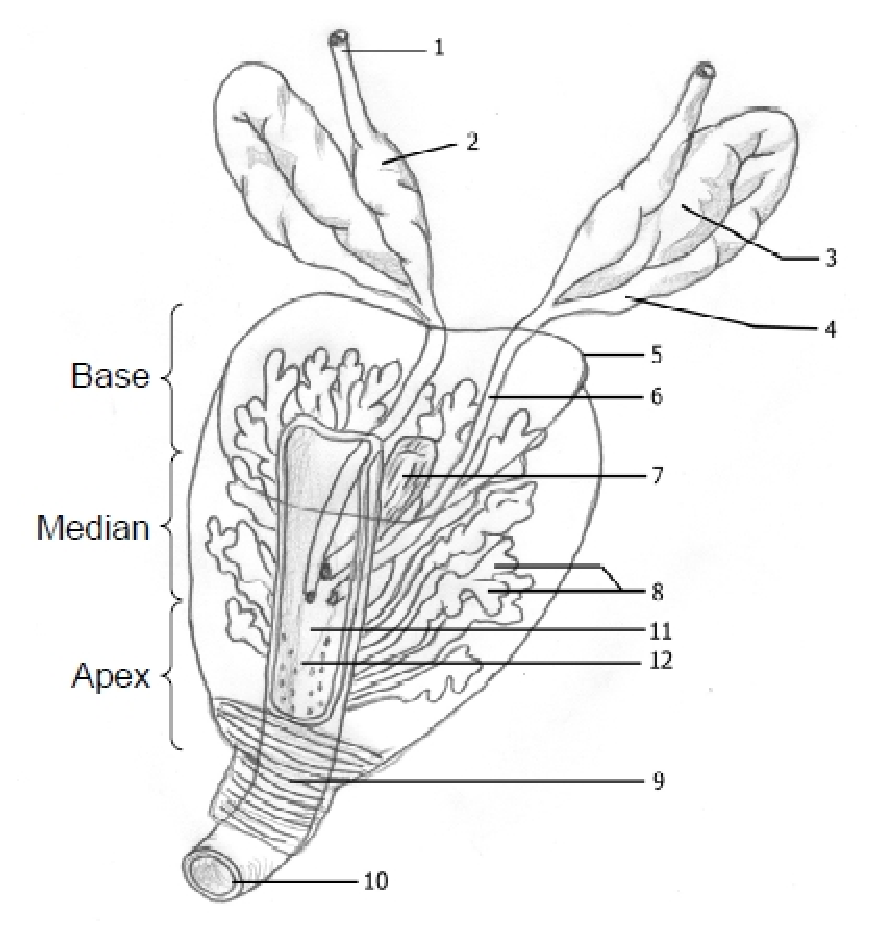
\includegraphics[width=0.50\textwidth]{anatomy/prostate2D2.eps}
%% 	\caption{Representation of the prostate. 1: Vas deferens, 2: Ampulla, 3: Seminal vesicle, 4: Excretory duct of seminal vesicle, 5: Prostate contour, 6: Ejaculatory duct, 7: Prostatic urticle, 8: Glandular tissue, 9: Urethral sphincter, 10: Urethra, 11: Seminal colliculus, 12: Urethral crest \cite{Wikipedia2011}.}
%% 	\label{fig:intro:prostatecancer:anatomy:anatomyProstate2D2}
%% \end{figure}


%% \begin{figure}
%% 	\centering
%% 	\subfigure[Transverse anatomy of the prostate.]{
%% 			\centering
%% 			\includegraphics[width=0.4\textwidth]{anatomy/prostateTransverse.eps}
%% 			\label{fig:anatomyProstateTransverse}}
%% 	~~~
%% 	\subfigure[Sagital anatomy of the prostate.]{
%% 			\centering
%% 			\includegraphics[width=0.4\textwidth]{anatomy/prostateSagital.eps}
%% 			\label{fig:anatomyProstateSagital}}
%% 	\caption{Presentation of the different zones of the prostate. \textit{AFT:} anterior fibromuscular tissue, \textit{CZ:} central zone, \textit{ED:} ejaculatory duct, \textit{NVB:} neurovascular bundle, \textit{PUT:} periurethral tissue, \textit{PZ:} peripherical zone, \textit{U:} urethra, \textit{TZ:} transitional zone \cite{Choi2007}.}
%% 	\label{fig:intro:prostatecancer:anatomy:anatomyProstateZone}
%% \end{figure}

\subsection{Prostate Carcinoma}
\ac{cap} has been reported on a worldwide scale to be the second most frequently diagnosed cancer of men accounting for $13.6 \%$ (\cite{Ferlay2010}). Statistically, in 2008, the number of new diagnosed cases was estimated to be $899,000$ with no less than $258,100$ deaths (\cite{Ferlay2010}). In United States, aside from skin cancer, \ac{cap} was declared to be the most commonly diagnosed cancer among men, implying that approximately one in six men will be diagnosed with \ac{cap} during their lifetime and one in thirty-six will die from this disease causing \ac{cap} to be the second most common cause of cancer death among men (\cite{Siegel2013}, \cite{Society2013}).

Despite active research to determine the causes of prostate cancer, a fuzzy list of risk factors has arisen (\cite{Society2010}). The etiology was linked to the following factors (\cite{Society2010}): (i) family history (\cite{Giovannucci2007,Steinberg1990}), (ii) genetic factors (\cite{Freedman2006,Amundadottir2006,Agalliu2009}), (iii) race-ethnicity (\cite{Giovannucci2007,Hoffman2001}), (iv) diet (\cite{Giovannucci2007,Ma2009,Alexander2010}), (v) obesity (\cite{Giovannucci2007,Rodriguez2007}). This list of risk factors alone cannot be used to diagnose CaP and in this way, screening enables early detection and treatment.

\ac{cap} growth is characterized by two main types of evolution (\cite{Strum2005}): slow-growing tumours, accounting for up to 85 \% of all \acp{cap} (\cite{Lu-Yao2009}), progress slowly and usually stay confined to the prostate gland. For such cases, treatment can be substituted with active surveillance. In contrast, the second variant of \acp{cap} develops rapidly and metastasises from prostate gland to others organs, primarily the bones (\cite{Oster2013}). Bone metastases, being an incurable disease, significantly affects the morbidity and mortality rate (\cite{Ye2007}). Hence, the  results of the surveillance have to be trustworthy in order to distinguish aggressive from slow-growing \ac{cap}.

\ac{cap} is more likely to come into being in specific regions of the prostate. In that respect, around 70-80 \% of \acp{cap} originate in \ac{pz} whereas 10-20 \% in \ac{tz} (\cite{Carrol1987,McNeal1988,Stamey1998}). Only about 5 \% of \acp{cap} occur in \ac{cz} (\cite{McNeal1988,Cohen2008}). However, those cancers appear to be more aggressive and more likely to invade other organs due to their location (\cite{Cohen2008}).


\subsection{Statistics}\label{subsection:intro:prostatecancer:statistics}

\subsubsection{Overview}\label{subsubsection:intro:prostatecancer:statistics:overview}

The World Health Organization (WHO) published in 2008 that PCa was the second most frequently diagnosed cancer of men and the fifth most common cancer overall \cite{Ferlay2010}. No less than 899,000 new cases where detected worldwide in 2008 \cite{Ferlay2010}. As presented on Fig. \ref{fig:intro:prostatecancer:statistics:overview:repartitionCancer}, PCa accounts for approximately 7.1\% (Fig. \ref{fig:intro:prostatecancer:statistics:overview:repartitionCancerIncidence}) of all cancers diagnosed in 2008 and 3.4\% (Fig. \ref{fig:intro:prostatecancer:statistics:overview:repartitionCancerDeaths}) of all cancers deaths in 2008 \cite{Ferlay2010}.

\begin{figure}
	\centering
	\subfigure[Estimated number cancers cases for both sexes and all ages.]{
			\centering
			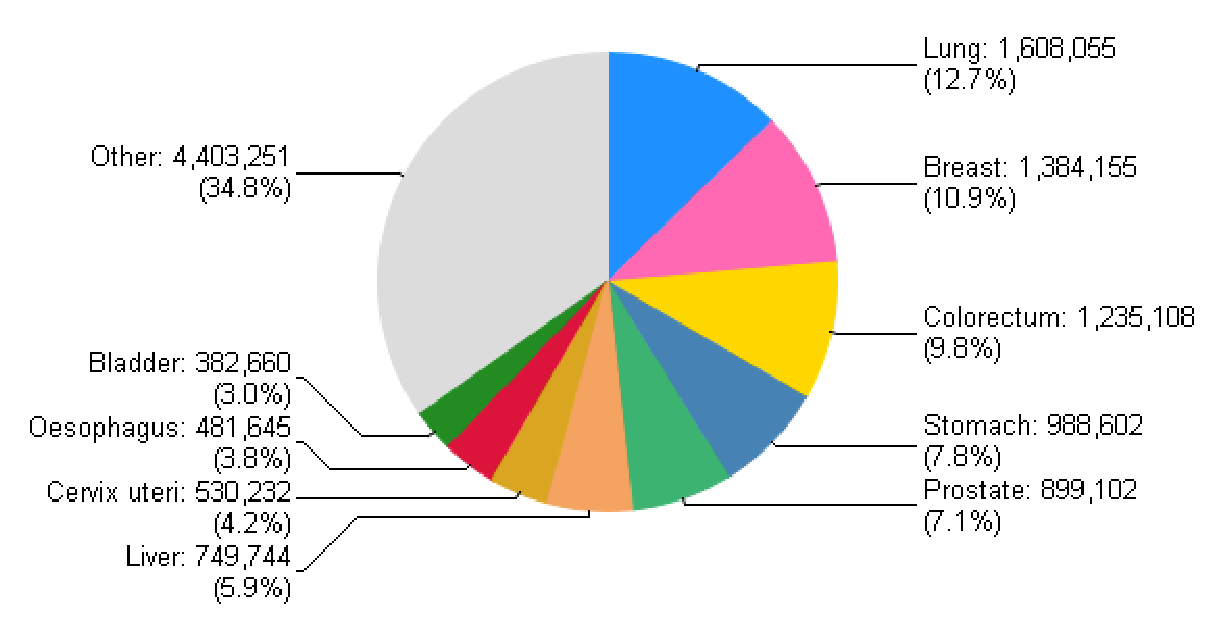
\includegraphics[width=0.65\textwidth]{statistics/repartitionCancerIncidence.eps}
			\label{fig:intro:prostatecancer:statistics:overview:repartitionCancerIncidence}}
	~
	\subfigure[Estimated number cancers deaths for both sexes and all ages.]{
			\centering
			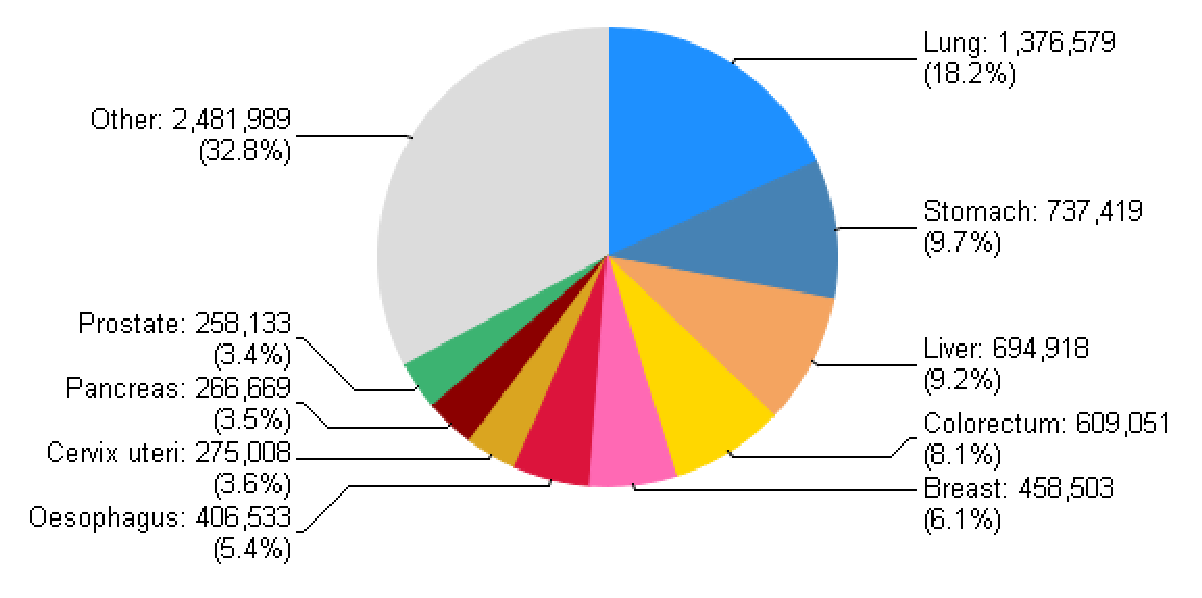
\includegraphics[width=0.65\textwidth]{statistics/repartitionCancerDeaths.eps}
			\label{fig:intro:prostatecancer:statistics:overview:repartitionCancerDeaths}}
	\caption{Cancer estimations in 2008 by the World Health Organization (WHO) \cite{Ferlay2010}.}
	\label{fig:intro:prostatecancer:statistics:overview:repartitionCancer}
\end{figure}

\subsubsection{Risk Factors}\label{subsubsection:intro:prostatecancer:statistics:riskfactors}

The risk factors can be categorized in three different classes: 

\begin{itemize}
	\item Age: age is the most important risk factor for PCa. The diagnosis of PCa for men over 50 years old. PCa rate increases upto about 70 and declines thereafter \cite{AmericanCancerSociety2010}.
	\item Genetic factors: it has been shown that the probability to have a cancer is higher when a member of the family has been already diagnosed \cite{AmericanCancerSociety2010}.
	\item Race: in the United States, the Africo Americans have a higher probability of developing a PCa than European American and Hispanic men \cite{AmericanCancerSociety2010}.
\end{itemize}

%%%%%%%%%%%%%%%%%%%%%%%%%% From previous draft %%%%%%%%%%%%%%%%%%%%%%%%%%%%%%%%%%%%%%%%%%%%%%%%
%% \subsection{Diagnosis and Medical Exams}\label{subsubsection:intro:prostatecancer:diagnosis}

%% The presence of PCa may be suggested in several ways: digital rectal examination, Prostate Specific Antigen (PSA\g) test, biopsy using transrectal ultrasound (TRUS\g) and magnetic resonance imaging (MRI\g-MRSI\g).

%% \subsubsection{Digital Rectal Examination}\label{subsubsection:intro:prostatecancer:diagnosis:rectalexamination}
%% Both benign prostatic hyperplasia and cancer may lead to an increasing size of the prostate. A rectal examination may allow detection of harder nodules within the softer prostatic tissue. The advantages are that this method is very fast and does not need any special equipment.
%% \subsubsection{PSA test}\label{subsubsection:intro:prostatecancer:diagnosis:psa}
%% The PSA is a protein secreted by the prostate. A higher-than-normal level of PSA can indicate an abnormality of the prostate: a benign prostatic hyperplasia or a cancer. However, other factors can lead to an increasing level of PSA such as prostate infections, irritations, a recent ejaculation or a recent rectal examination, etc.
%% The PSA can be found in the blood in two different forms: free PSA (about 10\%) and linked to another protein (about 90\%).
%% A level of PSA higher than 10 $ng.mL^{-1}$ is considered as pathologic \cite{Parfait2010}. If the PSA level is between 10 $ng.mL^{-1}$ and 4 $ng.mL^{-1}$, the patient is considered as suspicious \cite{Parfait2010}. In that case, the ratio free PSA over total PSA is computed. If the ratio is higher than 15\%, the case is considered as pathologic.
%% \subsubsection{TRUS}\label{subsubsection:intro:prostatecancer:diagnosis:trus}
%% As described in Sect. \ref{subsection:intro:prostatecancer:anatomy}, the prostate is localized in front of the rectum. Hence, its position allows one to carry out a biopsy using transrectal ultrasound (TRUS) in order to localise more precisely an eventual cancer (Fig. \ref{fig:intro:prostatecancer:diagnosis:trus}).
%% \textbf{\textit{\textsc{Add example of images of TRUS PCa and not}}}
%% \begin{figure}
%% 	\centering
%% 	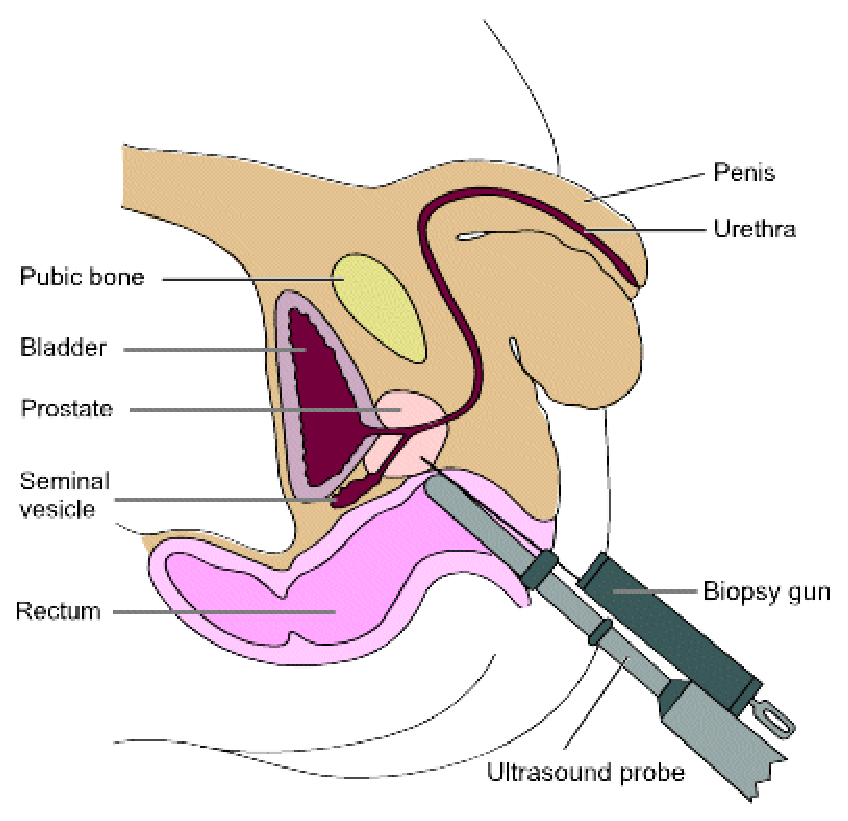
\includegraphics[width=0.45\textwidth]{diagnosis/trus/trus.eps}
%% 	\caption{Biopsy of the prostate using TRUS}
%% 	\label{fig:intro:prostatecancer:diagnosis:trus}
%% \end{figure}
%% \textbf{\textit{\textsc{Add information about protocol: manipulation of the patients, which equipment (see Jhimli thesis)}}}
%% The biopsy is usually prescribed when the PSA level is higher-than-normal or abnormalities were detected during a rectal examination. At least six different samples are taken from the right and left parts of the three different zones: apex, median and base. The samples are analysed in order to determine the presence of a cancer.
%% \textbf{\textit{\textsc{Add more information on the specificities and accuracy of the techniques. Add also what are the advantages (real-time)}}}

% MRI Principles:
%%% This part contains:
\section{Magnetic Resonance Imaging Principles}\label{section:intro:mriprinciples}



	% background information
\chapter{MRI Imaging Techniques}\label{chap:2}

% the code below specifies where the figures are stored
\ifpdf
    \graphicspath{{2_modality/figures/}}
\else
    \graphicspath{{2_modality/figures/}}
\fi

% Prostate Cancer:
%%% This part contains:
%%% - Anatomy basis of the prostate
%%% - Statistics regarding prostate cancers

%\section{MRI principles}\label{sec:chp2:principles}

\section{\acs*{mri} imaging techniques}\label{sec:chp2:imaging}

\ac{mri} provides promising imaging techniques to overcome the drawbacks of current clinical screening techniques mentioned in \acs{sec}\,\ref{chap:1}.
Unlike \ac{trus} biopsy, \ac{mri} examination is a non-invasive protocol and has been shown to be the most acute and harmless technique available currently~\cite{Turkbey2012}.
In this section, we review different \ac{mri} imaging techniques developed for \ac{cap} detection and diagnosis.
Features strengthening each modality will receive particular attention together with their drawbacks.
Commonly, these features form the basis for developing analytic tools and automatic algorithms.
However, we refer the reader to \acs{sec}\,\ref{subsec:chp3:img-clas:CADX-fea-dec} for more details on automatic feature detection methods since they are part and parcel of the \acs{cad} framework.
Table~\ref{tab:modmri} provides an overview of the following discussion.
\begin{landscape}
\begin{table}
  \scriptsize
    \caption{Overview of the features associated with each \acs*{mri} modality used for medical diagnosis by radiologists. Acronyms: \acf{cap} - \acf{si} - \acf{gs}.}\label{tab:modmri}
    \begin{threeparttable}
      \centering
      \noindent
      \begin{tabularx}{\linewidth}{@{} l X X X l @{}}
        \toprule
        \textbf{Modality} & \textbf{Significant features} & \textbf{\acs*{cap}} & \textbf{Healthy tissue} & \textbf{\acs*{gs} correlation} \\
        \midrule
        \acs*{t2w}-\acs*{mri} & \acs*{si} & low-\acs*{si} in \acs*{pz}~\cite{Hricak1987} & intermediate to high-\acs*{si} in \acs*{pz}~\cite{Hricak1987} & +~\cite{Wang2008} \\ 
        & Shape & round or ill-defined mass in \acs*{pz}~\cite{Hricak1983} &  & 0 \\
        & \acs*{si} & low-\acs*{si} in \acs*{cg}~\cite{Akin2006,Barentsz2012} & low-\acs*{si} in \acs*{cg}~\cite{Akin2006,Barentsz2012} & 0 \\
        & Shape & homogeneous mass with ill-defined edges in \acs*{cg}~\cite{Akin2006, Barentsz2012} &  & 0 \\ \\
        T$_2$ map & \acs*{si} & low-\acs*{si}~\cite{Liney1996,Gibbs2001} & intermediate to high-\acs*{si}~\cite{Liney1996,Gibbs2001} & +~\cite{Liu2011,Liney1996,Liney1997}  \\ \\
        \acs*{dce} \acs*{mri} & Semi-quantitative features~\cite{Verma2012}: & & & \\
        & $-$ wash-in & faster & slower & 0 \\
        & $-$ wash-out & faster & slower & 0 \\
        & $-$ integral under the curve & higher & lower & 0 \\
        & $-$ maximum signal intensity & higher & lower & 0 \\
        & $-$ time-to-peak enhancement & faster & slower & 0 \\ \\
        & Quantitative features (Tofts' parameters~\cite{Tofts2010}): & & & \\
        & $-$ $\text{k}_{\text{ep}}$ & higher & lower & 0 \\
        & $-$ $\text{K}^{\text{trans}}$ & higher & lower & 0 \\ \\
        \acs*{dw} \acs*{mri} & \acs*{si} & higher-\acs*{si}~\cite{Huisman2003,Barentsz2012} & lower-\acs*{si}~\cite{Huisman2003,Barentsz2012} & + \\ \\ 
        \acs*{adc} map & \acs*{si} & low-\acs*{si}~\cite{Barentsz2012} & high-\acs*{si}~\cite{Barentsz2012} & +~\cite{Hambrock2011, Itou2011, Peng2013} \\ \\
        \acs*{mrsi}& Metabolites: & & & \\
        & Citrate (2.64 ppm)~\cite{Verma2010} & lower concentration~\cite{Awwad2012,Costello2006,Graaf2000} & higher concentration~\cite{Awwad2012,Costello2006,Graaf2000} & +~\cite{Giskeodegard2013} \\
        & Choline (3.21 ppm)~\cite{Verma2010} & higher concentration~\cite{Awwad2012,Costello2006,Graaf2000} & lower concentration~\cite{Awwad2012,Costello2006,Graaf2000} & 0~\cite{Giskeodegard2013} \\
        & Spermine (3.11 ppm)~\cite{Verma2010} & lower concentration~\cite{Awwad2012,Costello2006,Graaf2000} & higher concentration~\cite{Awwad2012,Costello2006,Graaf2000} & +~\cite{Giskeodegard2013} \\ \bottomrule
        
      \end{tabularx}
      \begin{tablenotes}
      \item Notes:
      \item + = significantly correlated;
      \item 0 = no correlation.
      \end{tablenotes}
    \end{threeparttable}
  \label{tab:modmri}
\end{table}
\end{landscape}

\begin{figure}
\begin{adjustwidth}{-1.5cm}{}
\centering
% Define block styles used later

\tikzstyle{module}=[draw, draw=blue!80, text width=10em, 
    text centered, minimum height=5em, minimum width = 13em, drop shadow, rounded corners,
    fill=blue!30]
    
\tikzstyle{vecArrow} = [thick, decoration={markings,mark=at position
   1 with {\arrow[semithick]{open triangle 60}}},
   double distance=1.4pt, shorten >= 5.5pt,
   preaction = {decorate},
   postaction = {draw,line width=1.4pt, white,shorten >= 4.5pt}]

% Define distances for bordering
\def\blockdist{1.5}
\def\edgedist{2.5}

\begin{tikzpicture}[node distance=3cm,thick,scale=0.6, every node/.style={scale=0.6},path image/.style={
path picture={
\node at (path picture bounding box.center) {
\includegraphics[width=1cm]{#1}
};}}]
\tikzstyle{conefill} = [path image=,fill opacity=0.8]
\node[module=above:pre] (pre) at (4.5,-2.6) {\large Pre-processing};
\node[module,below of=pre] (seg) {\large Segmentation};
\node[module,below of=seg] (reg) {\large Registration};

\draw[->] (pre)--(seg);
\draw[->] (seg)--(reg);

\begin{pgfonlayer}{background}
	\path (pre.west |- pre.north)+(-0.5,1.0+\blockdist) node (a) {};
    \path (reg.east |- reg.south)+(+0.5,-0.5) node (b) {};
          
    \path[fill=blue!10,rounded corners, draw=blue!20, dashed] (a) rectangle (b);
\end{pgfonlayer}
        
\path (pre.north) +(0,+\blockdist) node (bgreg) {\large Image regularization};

\begin{scope}[node distance=10cm]
	\node[module] (det) [below right=0cm and 3cm of pre] {\large Features detection};
\end{scope}
\begin{scope}[node distance=3.5cm]
	\node[module,above of=det] (roi) {\large ROIs\\detection/selection};
\end{scope}
\node[module,below of=det] (sel) {\large Features\\selection/extraction};
\node[module,below of=sel] (cla) {\large Features\\classification/fusion};

\draw[->] (roi)--(det);
\draw[->] (det)--(sel);
\draw[->] (sel)--(cla);

\begin{pgfonlayer}{background}
	\path (roi.west |- roi.north)+(-0.5,1.0+\blockdist) node (c) {};
    \path (cla.east |- cla.south)+(+0.5,-0.5) node (d) {};
          
    \path[fill=blue!10,rounded corners, draw=blue!20, dashed] (c) rectangle (d);
\end{pgfonlayer}

\path (roi.north) +(0,+\blockdist) node (bgfea) {\large Image classification};

\begin{pgfonlayer}{background}
	\path (roi.west |- roi.north)+(-0.25,0.8) node (c) {};
    \path (roi.east |- roi.south)+(+0.25,-0.25) node (d) {};
          
    \path[fill=blue!20,rounded corners, draw=blue!25, dashed] (c) rectangle (d);
\end{pgfonlayer}

\path (roi.west |- roi.north) +(.6,0.4) node (bgfea) {\large \textbf{CADe}};

\begin{pgfonlayer}{background}
	\path (det.west |- det.north)+(-0.25,0.8) node (c) {};
    \path (cla.east |- cla.south)+(+0.25,-0.25) node (d) {};
          
    \path[fill=blue!20,rounded corners, draw=blue!25, dashed] (c) rectangle (d);
\end{pgfonlayer}

\path (roi.west |- det.north) +(.6,0.4) node (bgfea) {\large \textbf{CADx}};     

% Define the place where the arrow should start anf finish
\path (seg.east |- seg.north)+(+0.5,0) node (e) {};
\path (sel.west |- seg.north)+(-0.5,0) node (f) {};

\draw[double distance =3pt,preaction={-triangle 90,thin,draw,shorten >=-1mm}] (e) -- (f) node[midway,above] {\large Regularized data};

\begin{scope}[yshift=-11,xshift=-86]
	% opacity to prevent graphical interference
	\transparent{0.6}\draw[path image=2_modality/figures/tikzimage/t2.eps] (0,0) rectangle (1.0,1.0);
	%\fill[white,fill opacity=0.6] (0,0) rectangle (1.0,1.0);
    %\draw[step=2mm, black, thin] (0,0) grid (1.0,1.0);
	%\draw[black,thin] (0,0) rectangle (1.0,1.0);
\end{scope}

\begin{scope}[yshift=-8,xshift=-83]
	%\fill[white,fill opacity=0.6] (0,0) rectangle (1.0,1.0);
	\transparent{0.6}\draw[path image=2_modality/figures/tikzimage/t2.eps] (0,0) rectangle (1.0,1.0);
    %\draw[step=2mm, black, thin] (0,0) grid (1.0,1.0);
	%\draw[black,thin] (0,0) rectangle (1.0,1.0);
\end{scope}

\begin{scope}[yshift=-5,xshift=-80]
	% opacity to prevent graphical interference
	%\fill[white,fill opacity=0.8] (0,0) rectangle (1.0,1.0);
	\transparent{0.8}\draw[path image=2_modality/figures/tikzimage/t2.eps] (0,0) rectangle (1.0,1.0);
    %\draw[step=2mm, black, thin] (0,0) grid (1.0,1.0);
	%\draw[black,thin] (0,0) rectangle (1.0,1.0);
	\path (0,0)+(-1.5,0.3) node {\large T$_2$-W \ac{mri}};
\end{scope}

\begin{scope}[yshift=-78,xshift=-86]
	% opacity to prevent graphical interference
	\transparent{0.6}\draw[path image=2_modality/figures/tikzimage/t2.eps] (0,0) rectangle (1.0,1.0);
%	\fill[white,fill opacity=0.6] (0,0) rectangle (1.0,1.0);
%    \draw[step=2mm, black, thin] (0,0) grid (1.0,1.0);
%	\draw[black,thin] (0,0) rectangle (1.0,1.0);
\end{scope}

\begin{scope}[yshift=-75,xshift=-83]
	\transparent{0.6}\draw[path image=2_modality/figures/tikzimage/t2.eps] (0,0) rectangle (1.0,1.0);
%	\fill[white,fill opacity=0.6] (0,0) rectangle (1.0,1.0);
%    \draw[step=2mm, black, thin] (0,0) grid (1.0,1.0);
%	\draw[black,thin] (0,0) rectangle (1.0,1.0);
\end{scope}

\begin{scope}[yshift=-72,xshift=-80]
	% opacity to prevent graphical interference
	\transparent{0.8}\draw[path image=2_modality/figures/tikzimage/t2.eps] (0,0) rectangle (1.0,1.0);
%	\fill[white,fill opacity=0.8] (0,0) rectangle (1.0,1.0);
%    \draw[step=2mm, black, thin] (0,0) grid (1.0,1.0);
%	\draw[black,thin] (0,0) rectangle (1.0,1.0);
	\path (0,0)+(-1.2,0.3) node {\large T$_2$ map};
\end{scope}

\begin{scope}[yshift=-151,xshift=-86]
	% opacity to prevent graphical interference
	\transparent{0.6}\draw[path image=2_modality/figures/tikzimage/dce.eps] (0,0) rectangle (1.0,1.0);
%	\fill[white,fill opacity=0.6] (0,0) rectangle (1.0,1.0);
%    \draw[step=2mm, black, thin] (0,0) grid (1.0,1.0);
%	\draw[black,thin] (0,0) rectangle (1.0,1.0);
\end{scope}

\begin{scope}[yshift=-148,xshift=-83]
\transparent{0.6}\draw[path image=2_modality/figures/tikzimage/dce.eps] (0,0) rectangle (1.0,1.0);
%	\fill[white,fill opacity=0.6] (0,0) rectangle (1.0,1.0);
%    \draw[step=2mm, black, thin] (0,0) grid (1.0,1.0);
%	\draw[black,thin] (0,0) rectangle (1.0,1.0);
\end{scope}

\begin{scope}[yshift=-145,xshift=-80]
	% opacity to prevent graphical interference
	\transparent{0.8}\draw[path image=2_modality/figures/tikzimage/dce.eps] (0,0) rectangle (1.0,1.0);
%	\fill[white,fill opacity=0.8] (0,0) rectangle (1.0,1.0);
%    \draw[step=2mm, black, thin] (0,0) grid (1.0,1.0);
%	\draw[black,thin] (0,0) rectangle (1.0,1.0);
	\path (0,0)+(-1.5,0.3) node {\large DCE \ac{mri}};
\end{scope}

\begin{scope}[yshift=-219,xshift=-86]
\transparent{0.6}\draw[path image=2_modality/figures/tikzimage/dwi1.eps] (0,0) rectangle (1.0,1.0);
	% opacity to prevent graphical interference
%	\fill[white,fill opacity=0.6] (0,0) rectangle (1.0,1.0);
%    \draw[step=2mm, black, thin] (0,0) grid (1.0,1.0);
%	\draw[black,thin] (0,0) rectangle (1.0,1.0);
\end{scope}

\begin{scope}[yshift=-215,xshift=-83]
\transparent{0.6}\draw[path image=2_modality/figures/tikzimage/dwi1.eps] (0,0) rectangle (1.0,1.0);
%	\fill[white,fill opacity=0.6] (0,0) rectangle (1.0,1.0);
%    \draw[step=2mm, black, thin] (0,0) grid (1.0,1.0);
%	\draw[black,thin] (0,0) rectangle (1.0,1.0);
\end{scope}

\begin{scope}[yshift=-212,xshift=-80]
\transparent{0.8}\draw[path image=2_modality/figures/tikzimage/dwi1.eps] (0,0) rectangle (1.0,1.0);
	% opacity to prevent graphical interference
%	\fill[white,fill opacity=0.8] (0,0) rectangle (1.0,1.0);
%    \draw[step=2mm, black, thin] (0,0) grid (1.0,1.0);
%	\draw[black,thin] (0,0) rectangle (1.0,1.0);
	\path (0,0)+(-1.5,0.3) node {\large DW \ac{mri}};
\end{scope}

\begin{scope}[yshift=-285,xshift=-86]
	% opacity to prevent graphical interference
	\transparent{0.6}\draw[path image=2_modality/figures/tikzimage/mrsi.eps] (0,0) rectangle (1.0,1.0);
%	\fill[white,fill opacity=0.6] (0,0) rectangle (1.0,1.0);
%    \draw[step=2mm, black, thin] (0,0) grid (1.0,1.0);
%	\draw[black,thin] (0,0) rectangle (1.0,1.0);
\end{scope}

\begin{scope}[yshift=-282,xshift=-83]
\transparent{0.6}\draw[path image=2_modality/figures/tikzimage/mrsi.eps] (0,0) rectangle (1.0,1.0);
%	\fill[white,fill opacity=0.6] (0,0) rectangle (1.0,1.0);
%    \draw[step=2mm, black, thin] (0,0) grid (1.0,1.0);
%	\draw[black,thin] (0,0) rectangle (1.0,1.0);
\end{scope}

\begin{scope}[yshift=-279,xshift=-80]
\transparent{0.8}\draw[path image=2_modality/figures/tikzimage/mrsi.eps] (0,0) rectangle (1.0,1.0);
	% opacity to prevent graphical interference
%	\fill[white,fill opacity=0.8] (0,0) rectangle (1.0,1.0);
%    \draw[step=2mm, black, thin] (0,0) grid (1.0,1.0);
%	\draw[black,thin] (0,0) rectangle (1.0,1.0);
	\path (0,0)+(-1,0.3) node {\large MRSI};
\end{scope}

\path (pre.west |- pre.north)+(-3.5,1.0+\blockdist) node (g) {};
\path (reg.west |- reg.south)+(-3.5,-0.5) node (h) {};

\draw[decorate,decoration={brace,raise=6pt,amplitude=10pt}, thick]
    (g)--(h) ;
    
\path (seg.west |- seg.north)+(-2.5,0) node (i) {};
\path (seg.west |- seg.north)+(-0.5,0) node (j) {};
   
\draw[double distance =3pt,preaction={-triangle 90,thin,draw,shorten >=-1mm}] (i) -- (j);   

\path (sel.east |- seg.north)+(2,0) node (k) {};
\path (sel.east |- seg.north)+(0.5,0) node (l) {};
   
\draw[double distance =3pt,preaction={-triangle 90,thin,draw,shorten >=-1mm}] (l) -- (k);  

%\path (det.east |- det.north)+(.5,1.0+\blockdist) node (k) {};
%\path (cla.east |- cla.south)+(.5,-0.5) node (l) {};
%    
%\draw[decorate,decoration={brace,raise=6pt,amplitude=10pt}, thick]
%    (k)--(l) ;
    
\begin{scope}[path image/.style={
path picture={
\node at (path picture bounding box.center) {
\includegraphics[width=3cm]{#1}
};}}]    
\begin{scope}[yshift=-180,xshift=560]
	% opacity to prevent graphical interference
	\transparent{0.6}\draw[path image=2_modality/figures/tikzimage/likeli.eps,very thin] (0,0) rectangle (3.0,3.0);
%	\fill[white,fill opacity=0.6] (0,0) rectangle (1.0,1.0);
%    \draw[step=2mm, black, thin] (0,0) grid (1.0,1.0);
%	\draw[black,thin] (0,0) rectangle (1.0,1.0);
\end{scope}

\begin{scope}[yshift=-175,xshift=570]
\transparent{0.6}\draw[path image=2_modality/figures/tikzimage/likeli.eps,very thin] (0,0) rectangle (3.0,3.0);
%	\fill[white,fill opacity=0.6] (0,0) rectangle (1.0,1.0);
%    \draw[step=2mm, black, thin] (0,0) grid (1.0,1.0);
%	\draw[black,thin] (0,0) rectangle (1.0,1.0);
\end{scope}

\begin{scope}[yshift=-170,xshift=580]
	% opacity to prevent graphical interference
	\transparent{0.8}\draw[path image=2_modality/figures/tikzimage/likeli.eps,very thin] (0,0) rectangle (3.0,3.0);
%	\fill[white,fill opacity=0.8] (0,0) rectangle (1.0,1.0);
%    \draw[step=2mm, black, thin] (0,0) grid (1.0,1.0);
%	\draw[black,thin] (0,0) rectangle (1.0,1.0);
	\path (0,0)+(+1,-1) node {\large Likelihood};
	\path (0,0)+(+1,-1.5) node {\large cancer};
	\path (0,0)+(+1,-2) node {\large map};
\end{scope}
\end{scope}
\end{tikzpicture}
\caption[\ac{cad} framework using multiparametric \ac{mri} images.]{\ac{cad} framework using \ac{mri} images. Multiparametric \ac{mri} images are provided as inputs. These data arise from heterogeneous sources and need to be regularized. Some studies do not consider this stage as mandatory and do not implement or only partly those processes (see \acs{tab} \ref{tab:sumpap}). A pre-processing stage is usually applied to standardize the intensity of images, reduce noise and artefacts. Then, in the image set, the prostate organ has to be segmented to focus the next processing stages only on that particular \ac{roi}. Moreover, prostate location can vary depending of the modality chosen. Therefore, the images are registered so that all segmented images will be in the same reference frame. Once the image regularisation performed, image classification can be carried out. First, a strategy defining \acp{roi} to focus on is decided. Then, distinctive features are extracted before to be post-processed to select the most salient features. Finally, these salient features will feed a classifier previously trained which will provide a likelihood cancer map associated with either \ac{cap} detection or diagnosis.}
\label{fig:wkfcad}
\end{adjustwidth}
\end{figure}


%% % We are using enumerate with a small margin and some indent to organize our thoughts by paragraphs.
%% \setenumerate{listparindent=\parindent,itemsep=10px}
%% \setlist{noitemsep}

\begin{figure}
\centering
	\hspace*{\fill}
	\subfigure[\ac{t2w}-\ac{mri} slice of an healthy prostate acquire with a 1.5 Tesla \ac{mri}. The blue contour represents the \ac{cg} while the \ac{pz} corresponds to the green contour.]{\label{subfig:t2whealthy}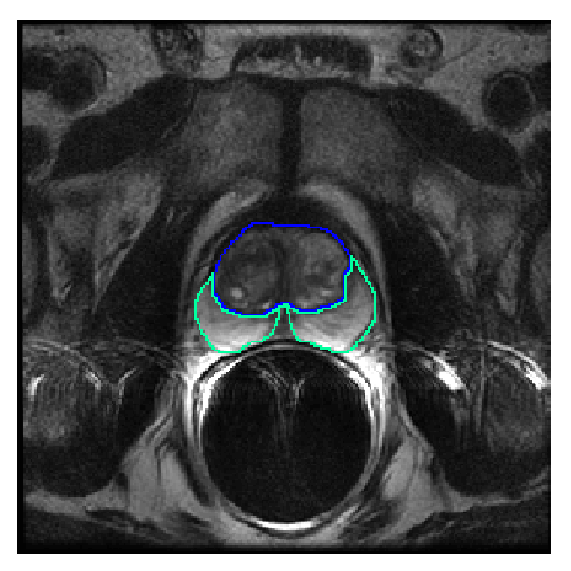
\includegraphics[width=0.3\linewidth]{2_modality/figures/t2w/t2w_healthy.eps}} \hfill
	\subfigure[\ac{t2w}-\ac{mri} slice of a prostate with a \ac{cap} highlighted in the \ac{pz} using a 3.0 Tesla \ac{mri} scanner.]{\label{subfig:t2wcancerpz}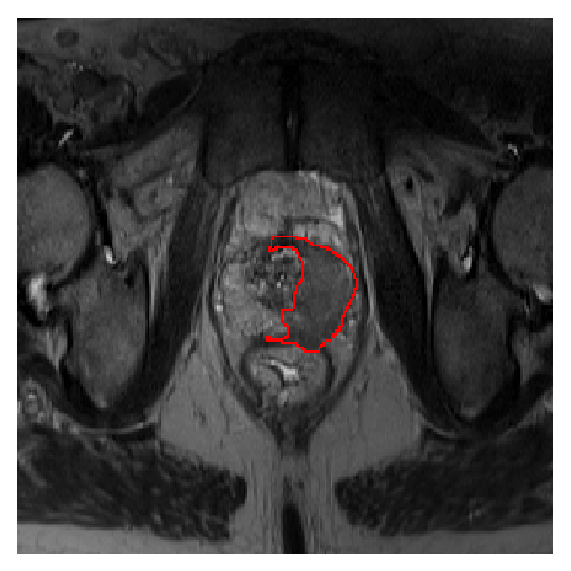
\includegraphics[width=0.3\linewidth]{2_modality/figures/t2w/t2w_cancer_pz.eps}} \hfill
	\subfigure[\ac{t2w}-\ac{mri} slice of a prostate with a \ac{cap} highlighted in the \ac{cg} using a 3.0 Tesla \ac{mri} scanner.]{\label{subfig:t2wcancercg}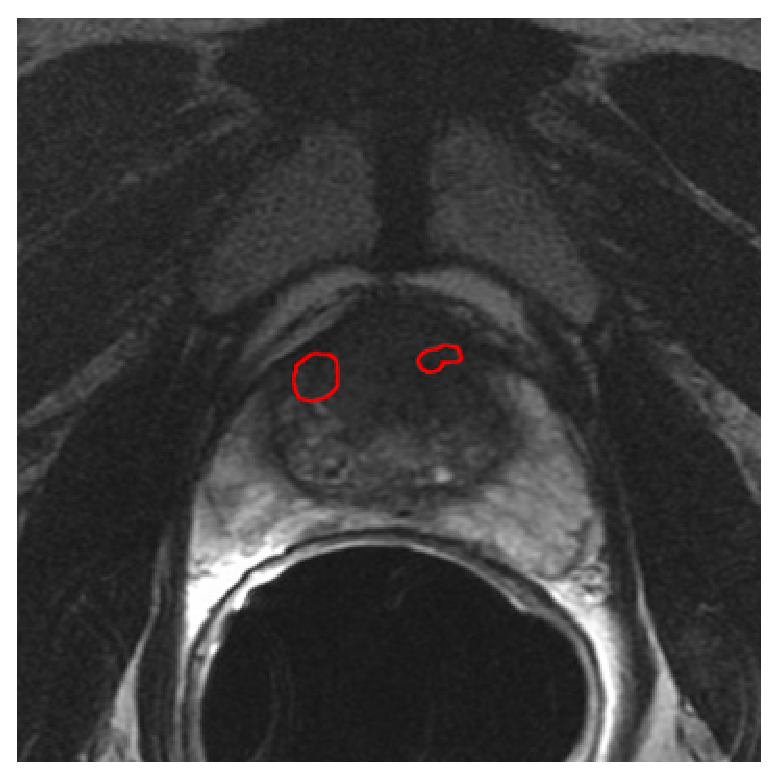
\includegraphics[width=0.3\linewidth]{2_modality/figures/t2w/t2w_cancer_cg.eps}}
	\hspace*{\fill}
	\caption[Rendering of \ac{t2w}-\ac{mri} prostate images.]{Rendering of \ac{t2w}-\ac{mri} prostate image with both 1.5 and 3.0 Tesla \ac{mri} scanner.}
	\label{fig:t2w}
\end{figure}

%T2W \ac{mri}
\subsection{\acs*{t2w} MRI}\label{subsec:chp2:imaging:t2w} 
\ac{t2w} \ac{mri} was the first \ac{mri}-modality used to perform \ac{cap} diagnosis using \ac{mri} \cite{Hricak1983}.
Nowadays, radiologists make use of it for \ac{cap} detection, localization and staging purposes.
This imaging technique is well suited to render zonal anatomy of the prostate \cite{Barentsz2012}. 

This modality relies on a sequence based on setting a long \ac{tr}, reducing the T$_{1}$ effect in \ac{nmr} signal measured, and fixing the \ac{te} to sufficiently large values in order to enhance the T$_{2}$ effect of tissues.
Thus, \ac{pz} and \ac{cg} tissues are well perceptible in these images.
The former is characterized by an intermediate/high-\ac{si} while the latter is depicted by a low-\ac{si} \cite{Hricak1987}.
An example of a healthy prostate is shown in Fig.~\ref{subfig:t2whealthy}.

In \ac{pz}, round or ill-defined low-SI masses are synonymous with \acp{cap} \cite{Hricak1983} as shown in Fig.~\ref{subfig:t2wcancerpz}.
Detecting \ac{cap} in \ac{cg} is more challenging.
In fact both normal \ac{cg} tissue and malignant tissue, have a low-\ac{si} in \ac{t2w} \ac{mri} reinforcing difficulties to distinguish between them.
However, \acp{cap} in \ac{cg} appear often as homogeneous mass possessing ill-defined edges with lenticular or ``water-drop'' shapes \cite{Akin2006, Barentsz2012} as depicted in Fig.~\ref{subfig:t2wcancercg}. 

\ac{cap} aggressiveness was shown to be inversely correlated with \ac{si}.
Indeed, \acp{cap} assessed with a \ac{gs} of 4-5 implied lower \ac{si} than the one with a \ac{gs} of 2-3 \cite{Wang2008}.

In spite of the availability of these useful and encouraging features, the \ac{t2w} modality lacks reliability \cite{Kirkham2006,Hoeks2011}.
Sensitivity is affected by the difficulties in detecting cancers in \ac{cg} \cite{Kirkham2006} while specificity rate is highly affected by outliers \cite{Barentsz2012}.
In fact, various conditions emulate patterns of \ac{cap} such as \ac{bph}, post-biopsy haemorrhage, atrophy, scars and post-treatment \cite{Hricak1987,Quint1991,Scheidler1999,Cruz2002,Barentsz2012}.
These issues can be partly addressed using more innovative and advanced modalities.

%T2 Map
\subsection{T$_2$ map} \label{subsec:chp2:imaging:t2}
As previously mentioned, \ac{t2w} \ac{mri} modality shows low sensitivity.
Moreover, \ac{t2w} \ac{mri} images are a composite of multiple effects \cite{Hegde2013}.
However, T$_2$ values alone have been shown to be more discriminative \cite{Liu2011} and highly correlated with citrate concentration, a biological marker in \ac{cap} \cite{Liney1996,Liney1997}. 

T$_2$ values are computed using the characteristics of transverse relaxation which is formalized as:

\begin{equation}
	M_{x,y}(t) = M_{x,y}(0) \exp \left( - \frac{t}{\text{T}_2} \right) \ ,
	\label{eq:tramag}
\end{equation}

\noindent where $M_{x,y}(0)$ is the initial value of $M_{x,y}(t)$ and T$_2$ is the relaxation time.
By rearranging \acs{eq}~\ref{eq:tramag}, T$_2$ map is computed performing a linear fitting on the model in \acs{eq}~\ref{eq:t2map} using several TE, $t=\{ \text{TE}_1,\text{TE}_2, \dotsc ,\text{TE}_m \}$.

\begin{equation}
	\ln \left[ \frac{M_{x,y}(t)}{M_{x,y}(0)} \right] = - \frac{t}{\text{T}_2} \ .
	\label{eq:t2map}
\end{equation}

The \Ac{fse} sequence has been shown to be particularly well suited in order to build a T$_2$ map and obtain accurate T$_2$ values \cite{Liney1996a}.
Similar to \ac{t2w} \ac{mri}, T$_2$ values associated with \ac{cap} are significantly lower than those of healthy tissues \cite{Liney1996,Gibbs2001}.

\begin{figure}
\centering
	\hspace*{\fill}
	\subfigure[\ac{t1w}-\ac{mri} image where the cancer is delimited by the red contour. The green area was still not invaded by the \ac{cap}]{\label{subfig:t1w}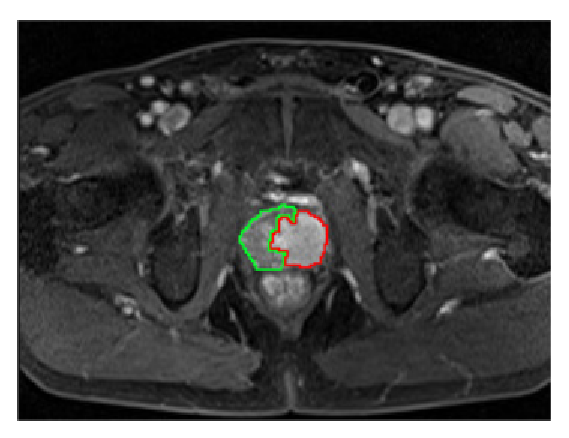
\includegraphics[width=0.4\linewidth]{2_modality/figures/dce/slice.eps}} \hfill
	\subfigure[Enhancement curve computed during the \ac{dce}-\ac{mri} analysis. The red curve is typical from \ac{cap} cancer while the green curve is characteristic of healthy tissue.]{\label{subfig:dce}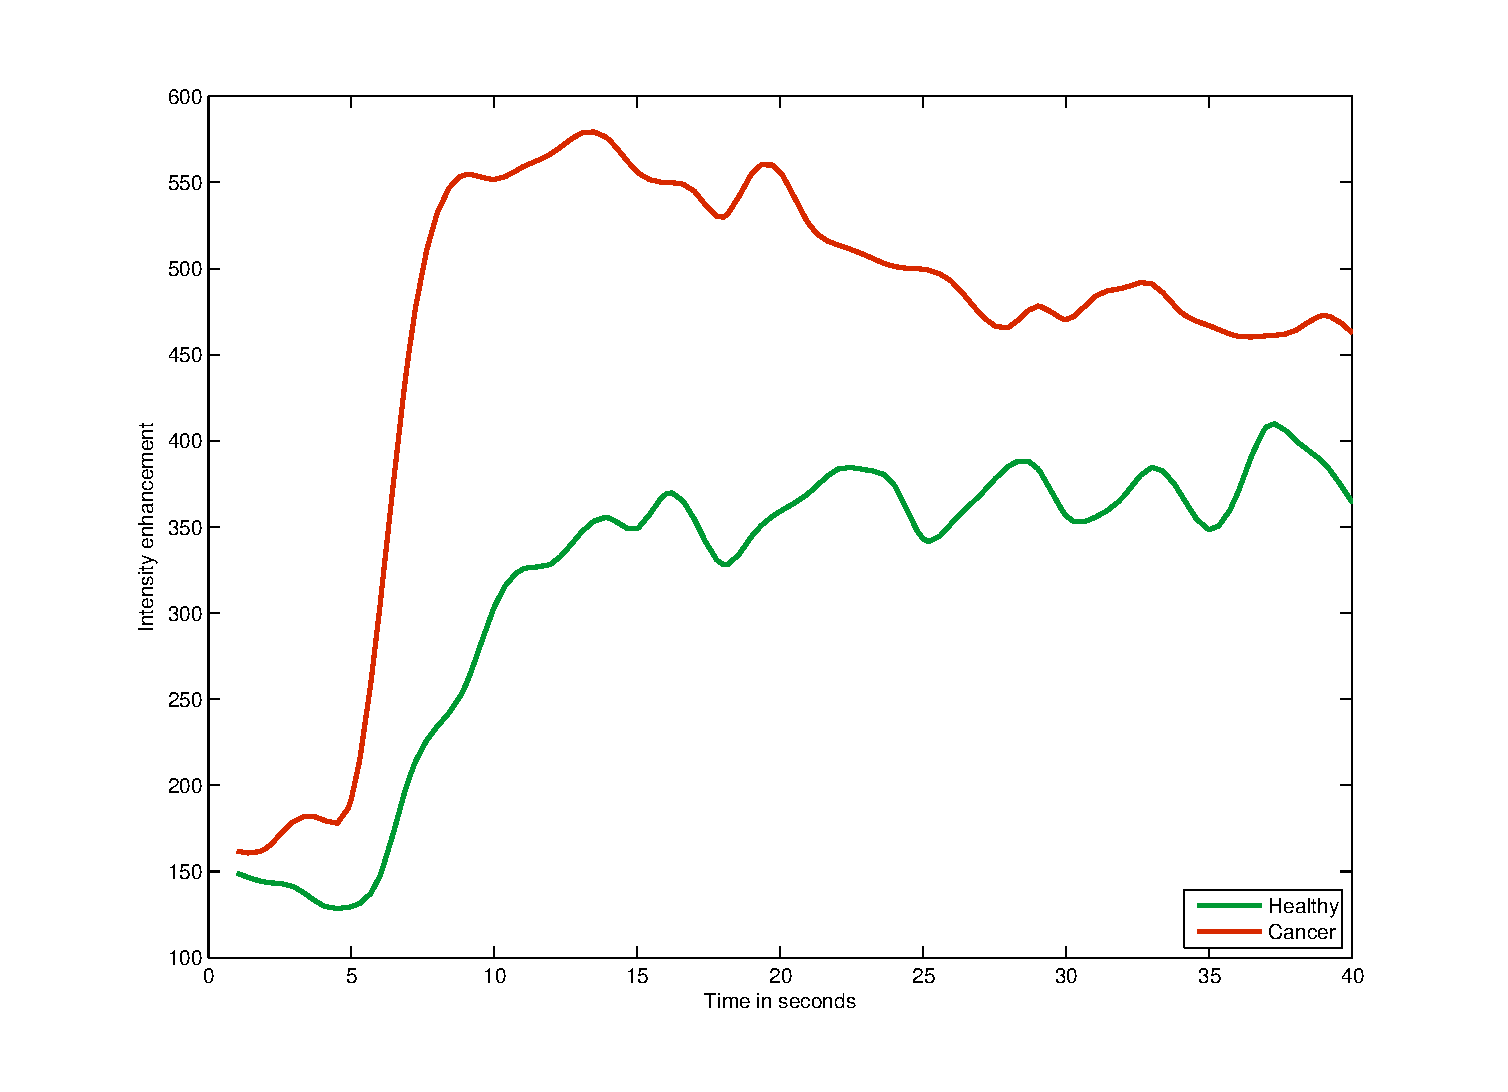
\includegraphics[width=0.45\linewidth]{2_modality/figures/dce/dce_cancer_healthy.eps}}
	\hspace*{\fill}
	\caption[Enhancement of \ac{dce}-\ac{mri} signal.]{Illustration of typical enhancement signal observed in \ac{dce}-\ac{mri} analysis collected with a 3.0 Tesla \ac{mri} scanner.}
	\label{fig:dceana}
\end{figure}

%DCE \ac{mri}
\subsection{\acs*{dce} \ac{mri}}\label{subsec:chp2:imaging:dce}
\ac{dce} \ac{mri} is an imaging technique which exploits the vascularity characteristic of tissues.
Contrast media, usually gadolinium-based, is injected intravenously into the patient.
The media extravasates from vessels to \ac{ees} and is released back into the vasculature before being eliminated by the kidneys \cite{Gribbestad2005}.
Furthermore, the diffusion speed of the contrast agent may vary due to several parameters: (i) the permeability of the micro-vessels, (ii) their surface area and (iii) the blood flow \cite{Padhani2002}.

Healthy \ac{pz} is mainly made up of glandular tissue, around 70 \% \cite{Choi2007}, which implies a reduced interstitial space restricting exchanges between vessels and \ac{ees} \cite{Buckley2004,Niekerk2009}.
Normal \ac{cg} has a more disorganised structure, composed of mainly fibrous tissue \cite{Choi2007,Hoeks2011}, which facilitates the arrival of the contrast agent in \ac{ees} \cite{Niekerk2013}.
To understand the difference between contrast media kinetic in malignant tumours and the two previous behaviours mentioned, one has to focus on the process known as angiogenesis \cite{Carmeliet2000}.
In order to ensure growth, malignant tumours produce and release angiogenic promoter substances \cite{Carmeliet2000}.
These molecules stimulate the creation of new vessels towards the tumour \cite{Carmeliet2000}.
However, the new vessel networks in tumours differ from those present in healthy tissue \cite{Gribbestad2005}.
They are more porous due to the fact that their capillary walls have a large number of ``openings'' \cite{Gribbestad2005,Choi2007}.
In contrast to healthy cases, this increased vascular permeability results in increased contrast agent exchanges between vessels and \ac{ees} \cite{Verma2012}.

By making use of the previous aspects, \ac{dce} \ac{mri} is based on an acquisition of a set of \ac{t1w} \ac{mri} images over time.
The Gadolinium-based contrast agent shortens T$_1$ relaxation time enhancing contrast in \ac{t1w} \ac{mri} images.
The aim is to post-analyse the pharmacokinetic behaviour of the contrast media concentration in prostate tissues \cite{Verma2012}.
The image analysis is carried out in two dimensions: (i) in the spatial domain on a pixel-by-pixel basis and (ii) in the time domain corresponding to the consecutive images acquired with the \ac{mri}.
Thus, for each spatial location, a signal linked to contrast media concentration is measured as shown in Fig.~\ref{subfig:dce} \cite{Tofts2010}. 

By taking the previous remarks regarding medical aspects and signal theory into account, \acp{cap} are characterized by a signal having an earlier and faster enhancement and an earlier wash-out (cf., the rate of the contrast agent flowing out of the tissue) (see Fig.~\ref{subfig:dce}) \cite{Verma2012}.
Three different approaches exist to analyse these signals with the aim of tagging them as corresponding to either normal or malignant tissues.
Qualitative analysis is based on assessment of the signal shape \cite{Hoeks2011}.

Quantitative approaches consist of inferring pharmocokinetic parameter values \cite{Tofts2010}.
Those parameters are part of mathematical-pharmacokinetic models which are directly based on physiological exchanges between vessels and \ac{ees}.
Several pharmacokinetic models were proposed such as the Kety model \cite{Kety1951}, the Tofts model \cite{Tofts1997} and mixed models \cite{Larsson1996,StLawrence1998}.
The last family of methods mixed both approaches and are grouped together under the heading of semi-quantitative methods.
They rely on shape characterization using mathematical modelling to extract a set of parameters such as wash-in gradient, wash-out, integral under the curve, maximum signal intensity, time-to-peak enhancement and start of enhancement.
These parameters will be discussed in a later section (see Fig.~\ref{fig:dceparam}) \cite{Hoeks2011,Verma2012}.
It was shown that semi-quantitative and quantitative methods improve localization of \ac{cap} when compared with qualitative methods \cite{Rosenkrantz2013}.
Section~\ref{subsubsec:fddce} provides a full description of quantitative and semi-quantitative approaches.


\ac{dce} \ac{mri} combined with \ac{t2w} \ac{mri} has shown to enhance sensitivity compared to \ac{t2w} \ac{mri} alone \cite{Jager1997,Kim2005,Schlemmer2004,Zelhof2009}.
Despite this fact, \ac{dce} \ac{mri} possesses some drawbacks.
Due to its ``dynamic'' nature, patient motions during the image acquisition lead to spatial misregistration of the image set \cite{Verma2012}).
Furthermore, it has been suggested that malignant tumours are difficult to distinguish from prostatitis located in \ac{pz} and \ac{bph} located in \ac{cg} \cite{Hoeks2011,Verma2012}.
These pairs of tissues tend to have similar appearances. Later studies have shown that \acp{cap} in \ac{cg} do not always manifest in homogeneous fashion.
Indeed, tumours in this zone can present both hypo-vascularization and hyper-vascularization which illustrates the challenge of \ac{cap} detection in \ac{cg} \cite{Niekerk2013}.

\begin{figure}
\centering
	\hspace*{\fill}
	\subfigure[\ac{dw}-\ac{mri} image acquired with a 1.5 Tesla \ac{mri} scanner. The cancer corresponds to the high \ac{si} region highlighted in red.]{\label{subfig:dwi}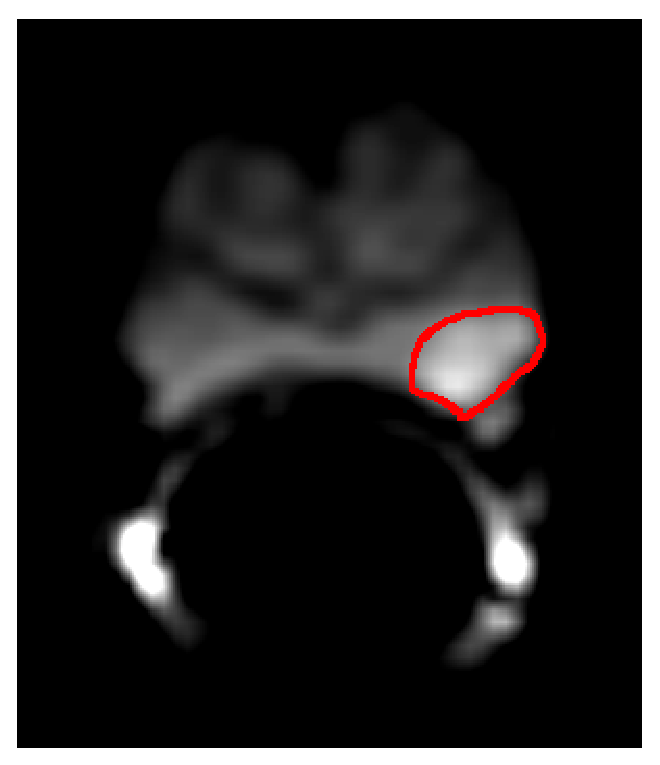
\includegraphics[width=0.25\linewidth]{2_modality/figures/dwi/dwi_cancer.eps}} \hfill
	\subfigure[\ac{adc} map computer after acquisition of \ac{dw}-\ac{mri} iages with a 1.5 Tesla \ac{mri} scanner. The cancer corresponds to the low \ac{si} region highlighted in red.]{\label{subfig:adc}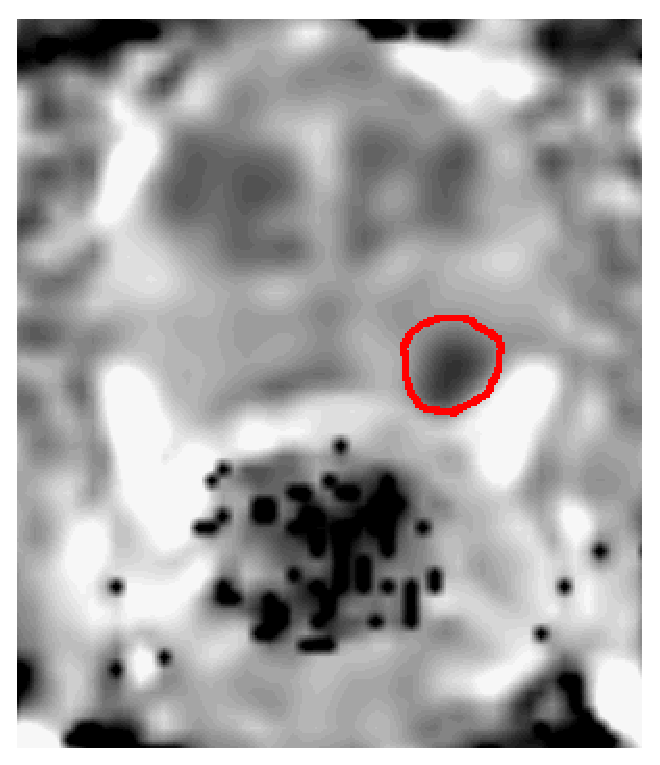
\includegraphics[width=0.25\linewidth]{2_modality/figures/dwi/adc_cancer.eps}}
	\hspace*{\fill}
	\caption[Example of \ac{dw}-\ac{mri} and \ac{dce} map.]{Illustration of of \ac{dw}-\ac{mri} and \ac{adc} map. The signal intensity corresponding to cancer are inversely correlated on these two types of imaging techniques.}
	\label{fig:dwi}
\end{figure}

%DWI \ac{mri}
\subsection{\acs*{dw} \ac{mri}}\label{subsec:chp2:imaging:dw}
As previously mentioned in the introduction, \ac{dw} \ac{mri} is the most recent \ac{mri} imaging technique aiming at \ac{cap} detection and diagnosis \cite{Scheidler1999}.
This modality exploits the variations in the motion of water molecules in different tissues \cite{LeBihan1988,Koh2007}.

From a physiological point of view, the following facts can be claimed.
On the one hand, \ac{pz}, as previously mentioned, is mainly glandular and tubular in structure allowing water molecules to move freely \cite{Choi2007,Hoeks2011}.
On the other hand, \ac{cg} is made up of muscular or fibrous tissue causing the motion of the water molecules to be more constrained and heterogeneous than in \ac{pz} \cite{Hoeks2011}.
Then, \ac{cap} growth leads to the destruction of normal glandular structure and is associated with an increase in cellular density \cite{Hoeks2011,Koh2007,Somford2008}.
Furthermore, these factors both have been shown to be inversely correlated with water diffusion \cite{Koh2007,Somford2008}: higher cellular density implies a restricted water diffusion.
Thus, water diffusion in \ac{cap} will be more restricted than both healthy \ac{pz} and \ac{cg} \cite{Koh2007,Hoeks2011}.

From the \ac{nmr} principle side, \ac{dw} \ac{mri} sequence produces contrasted images due to variation of water molecules motion.
The method is based on the fact that the signal in \ac{dw} \ac{mri} images is inversely correlated to the degree of random motion of water molecules \cite{Huisman2003}.
In fact, gradients are used in \ac{dw} \ac{mri} modality to encode spatial location of nuclei temporarily.
Simplifying the problem in only one direction, a gradient is applied in that direction, dephasing the spins of water nuclei.
Hence, the spin phases vary along the gradient direction depending of the gradient intensity at those locations.
Then, a second gradient is applied aiming at cancelling the spin dephasing.
Thus, the immobile water molecules will be subject to the same gradient intensity as the initial one while moving water molecules will be subject to a different gradient intensity.
Thus, spins of moving water molecules will stay dephased whereas spins of immobile water molecules will come back in phase.
As a consequence, a higher degree of random motion results in a more significant signal loss whereas a lower degree of random motion is synonymous with lower signal loss \cite{Huisman2003}.
Under these conditions, the \ac{mri} signal is measured as:

\begin{equation}
	M_{x,y}\left(t,b\right) = M_{x,y}(0) \exp \left( - \frac{t}{\text{T}_2} \right) S_{\text{ADC}}(b) \ , 
	\label{eq:t2dif}
\end{equation}

\begin{equation}
	S_{\text{ADC}}(b) = \exp \left( -b \times \text{ADC} \right) \ ,
	\label{eq:dif}
\end{equation}

\noindent where $S_{\text{ADC}}$ refers to signal drop due to diffusion effect, $\text{ADC}$ is the \acl{adc} and $b$ is the attenuation coefficient depending only on gradient pulses parameters: (i) gradient intensity and (ii) gradient duration \cite{LeBihan1986}.

By using this formulation, image acquisition with a parameter $b=0$ s.mm$^{-2}$ corresponds to a \ac{t2w} \ac{mri} acquisition.
Then, increasing the attenuation coefficient $b$ (cf., increase gradient intensity and duration) enhances the contrast in \ac{dw} \ac{mri} images.

To summarize, in \ac{dw} \ac{mri} images, \acp{cap} are characterized by high-\ac{si} compared to normal tissues in \ac{pz} and \ac{cg} as shown in Fig.~\ref{subfig:dwi} \cite{Barentsz2012}.
However, some tissues in \ac{cg} can look similar to \ac{cap} with higher \ac{si} \cite{Barentsz2012}.

Diagnosis using \ac{dw} \ac{mri} combined with \ac{t2w} \ac{mri} has shown a significant improvement compared with \ac{t2w} \ac{mri} alone and provides highly contrasted images \cite{Shimofusa2005,Padhani2011,Choi2007}.
As drawbacks, this modality suffers from poor spatial resolution and specificity due to false positive detection \cite{Choi2007}.
With a view to eliminate these drawbacks, radiologists are extracting quantitative maps from \ac{dw} \ac{mri}.
This imaging technique is presented next.

%ADC map
\subsection{\acs*{adc} Map}\label{subsec:chp2:imaging:adc} 
The \ac{nmr} signal measured for \ac{dw} \ac{mri} images is not only affected by diffusion as shown in \acs{eq} \eqref{eq:t2dif}.
However, the signal drop (\acs{eq} \eqref{eq:dif}) is formulated such that the only variable is the acquisition parameter $b$ \cite{LeBihan1986}.
The \ac{adc} is considered as a ``pure'' diffusion coefficient and can be extracted to build a quantitative map.

From \acs{eq} \eqref{eq:t2dif}, it is clear that performing multiple acquisitions only varying $b$ will not have any effect on the term  $M_{x,y}(0) \exp \left( - \frac{t}{\text{T}_2} \right)$.
Thus, \acs{eq} \eqref{eq:t2dif} can be rewritten as:

\begin{equation}
	S(b) = S_0 \exp \left( -b \times \text{ADC} \right) \ .
	\label{eq:t2adcrew}
\end{equation}

To compute the \ac{adc} map, a minimum of two acquisitions are necessary: (i) for $b_0=0$ s.mm$^{-2}$ where the measured signal is equal to $S_0$, and (ii) $b_1>0$ s.mm$^{-2}$ (typically $1000$ s.mm$^{-2}$).
Then, the \ac{adc} map can be computed as:

\begin{equation}
	\text{ADC} = - \frac{\ln \left( \cfrac{S(b_1)}{S_0} \right) }{b_1} \ .
	\label{eq:adcres1}
\end{equation}

More accurate computation of the \ac{adc} map can be obtained by performing several acquisitions with different values for the parameter $b$ and performing a semi-logarithmic linear fitting using the model presented in \acs{eq} \eqref{eq:t2adcrew}.

Regarding the appearance of the \ac{adc} maps, it was previously stated that by increasing the value of $b$, the signal of \ac{cap} tissue increases significantly.
From \acs{eq} \eqref{eq:adcres1}, it can be shown that tissue appearance in the ADC map will be the inverse of \ac{dw} \ac{mri} images.
Then, \ac{cap} tissue is associated with low-\ac{si} whereas healthy tissue appears brighter as depicted in Fig.~\ref{subfig:adc} \cite{Barentsz2012}.

Similar to the gain achieved by \ac{dw} \ac{mri}, diagnosis using \ac{adc} map combined with \ac{t2w} \ac{mri} significantly outperforms \ac{t2w} \ac{mri} alone \cite{Doo2012,Choi2007}.
Moreover, it has been shown that \ac{adc} is correlated with \ac{gs} \cite{Hambrock2011, Itou2011, Peng2013}.

However, some tissues of the \ac{cg} zone mimic \ac{cap} with low-\ac{si} \cite{Kirkham2006} and image distortion can arise due to haemorrhage \cite{Choi2007}.
It has also been noted that a high variability of the \ac{adc} occurs between different patients making it difficult to define a static threshold to distinguish \ac{cap} from non-malignant tumours \cite{Choi2007}. 

\begin{figure}
	\centering
	\hspace*{\fill}
	\subfigure[Illustration of an \ac{mrsi} spectrum of an healthy voxel acquired with a 3.0 Tesla \ac{mri}.]{\label{subfig:mrsihea}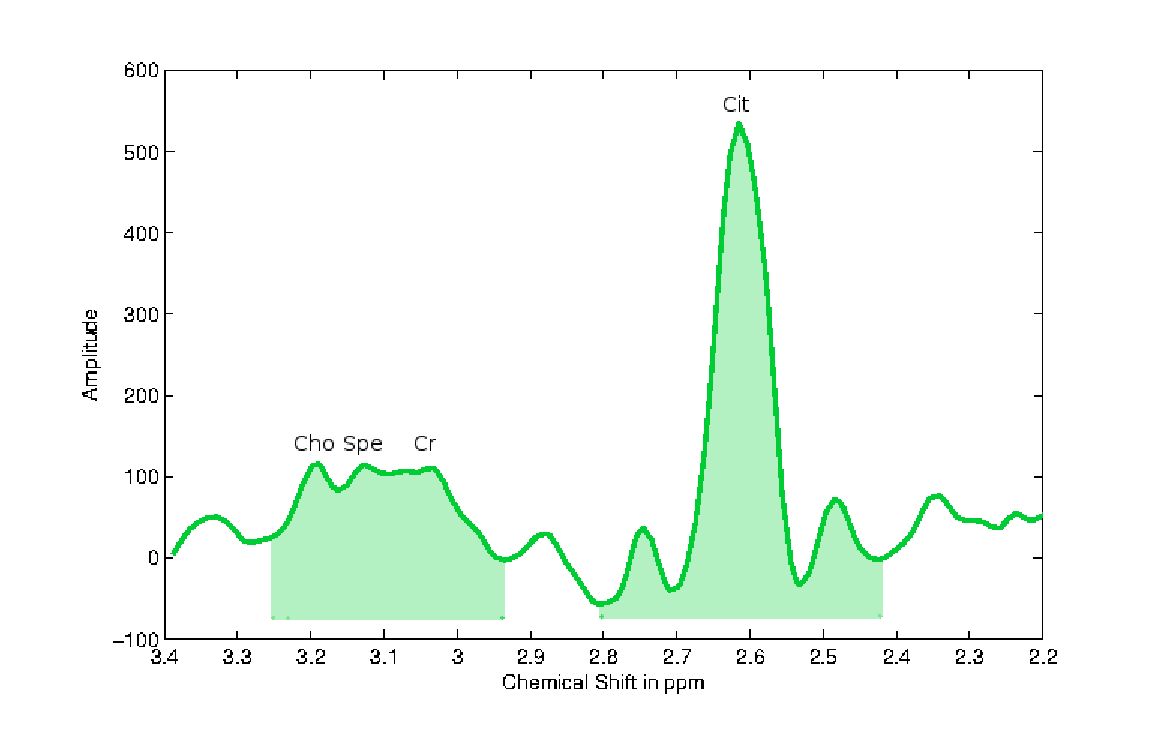
\includegraphics[width=0.45\linewidth]{2_modality/figures/mrsi/mrsi_healthy.eps}} \hfill
	\subfigure[Illustration of an \ac{mrsi} spectrum of a cancerous voxel acquired with a 3.0 Tesla \ac{mri}.]{\label{subfig:mrsican}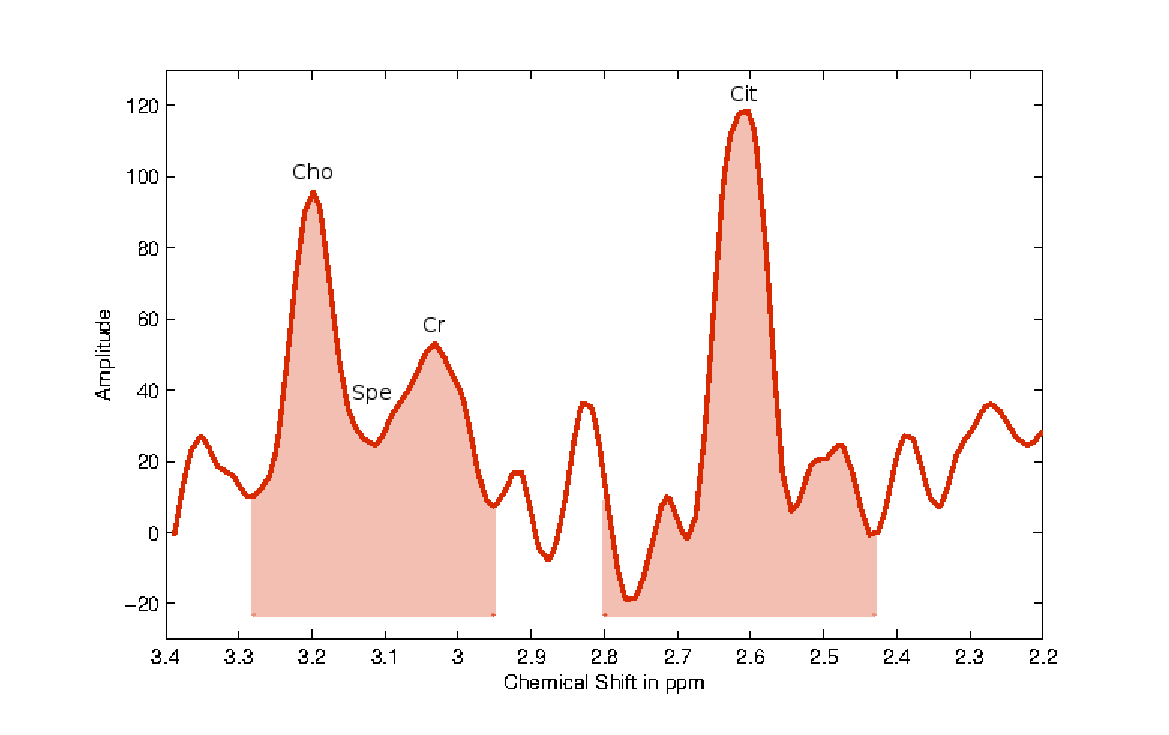
\includegraphics[width=0.45\linewidth]{2_modality/figures/mrsi/mrsi_cancer.eps}}
	\hspace*{\fill}
	\caption[Illustration of healthy and cancerous \ac{mrsi} spectrum.]{Illustration of an \ac{mrsi} spectrum both healthy and cancerous voxel with a 3.0 Tesla \ac{mri}. The highlighted areas corresponds to the related concentration of the metabolites which is computed by integrating the area under each peak. Acronyms: Choline (Cho), Spermine (Spe), Creatine (Cr) and Citrate (Cit).}
	\label{fig:mrsi}
\end{figure}


%MRSI
\subsection{\acs*{mrsi}}\label{subsec:chp2:imaging:mrsi}
\ac{cap} induces metabolic changes in the prostate compared with healthy tissue.
Thus, \ac{cap} detection can be carried out by tracking changes of metabolite concentration in prostate tissue.
\ac{mrsi} is an \ac{nmr}-based technique which generates spectra of relative metabolite concentration in \iac{roi}.

In order to track changes of metabolite concentration, it is important to know which metabolites are associated with \ac{cap}.
To address this question, clinical studies identified three biological markers: (i) citrate, (ii) choline and (iii) polyamines composed mainly of spermine, and in less abundance of spermidine and putrescine \cite{Awwad2012,Costello2006,Giskeodegard2013}. 

Citrate is involved in the production and secretion of the prostatic fluid, and the glandular prostate cells are associated with a high production of citrate enabled by zinc accumulation by these same cells \cite{Costello2006}.
However, the metabolism allowing the accumulation of citrate requires a large amount of energy \cite{Costello2006}.
In contrast, malignant cells do not have high zinc levels leading to lower citrate levels due to citrate oxydation \cite{Costello2006}.
Furthermore, this change results in a more energy-efficient metabolism enabling malignant cells to grow and spread \cite{Costello2006}.

An increased concentration of choline is related to \ac{cap} \cite{Awwad2012}.
Malignant cell development requires epigenetic mechanisms resulting in metabolic changes and relies on two mechanisms: DNA methylation and phospholid metabolism which both result in choline uptake, explaining its increased level in \ac{cap} tissue \cite{Awwad2012}.
Spermine is also considered as a biological marker in \ac{cap} \cite{Graaf2000,Giskeodegard2013}.
In \ac{cap}, reduction of the ductal volume due to shifts in polyamine homeostasis might lead to a reduced spermine concentration \cite{Graaf2000}.

To determine the concentration of these biological markers, one has to focus on the \ac{mrsi} modality.
In theory, in presence of a homogeneous magnetic field, identical nuclei precesses at the same operating frequency known as the Lamor frequency \cite{Haacke1999}.
However, \ac{mrsi} is based on the fact that identical nuclei will slightly precess at different frequencies depending on the chemical environment in which they are immersed \cite{Haacke1999}, a phenomenon known as the \ac{cse} \cite{Parfait2010}.
Given this property, metabolites can be identified and their concentrations can be determined.
In this regard, the Fourier transform is used to obtain the frequency spectrum of the \ac{nmr} signal \cite{Haacke1999,Parfait2010}.
In this spectrum, each peak is associated with a particular metabolite and the area under each peak corresponds to the relative concentration of this metabolite (see Fig.~\ref{fig:mrsi}) \cite{Parfait2010}.

Two different quantitative approaches are used to decide or whether not the spectra of \iac{roi} is associated with \ac{cap} classified either as relative quantification or absolute quantification \cite{Lemaitre2011}.
In relative quantification, the ratio of choline-polyamines-creatine to citrate is computed.
The integral of the signal is computed from choline (cf., 3.21 ppm) to creatine (cf., 3.02 ppm) because the peaks in this region can be merged at clinical magnetic field strengths (see Fig.~\ref{fig:mrsi}) \cite{Hoeks2011,Graaf2000}.
Considering the previous assumption that choline concentration rises and citrate concentration decreases in the presence of \ac{cap}, the ratio computed should be higher in malignant tissue than in healthy tissue. 

Two different quantitative approaches are used to decide or not the spectra of \iac{roi} is associated with \ac{cap} classified either as relative quantification or absolute quantification \cite{Lemaitre2011}.
In relative quantification, the ratio of choline-polyamines-creatine to citrate is computed.
The integral of the signal is computed from choline (cf., 3.21 ppm) to creatine (cf., 3.02 ppm) because the peaks in this region can be merged at clinical magnetic field strengths (see Fig.~\ref{fig:mrsi}) \cite{Hoeks2011,Graaf2000}.
Considering the previous assumption that choline concentration rises and citrate concentration decreases in the presence of \ac{cap}, the ratio computed should be higher in malignant tissue than in healthy tissue. 

In contrast with relative quantification, absolute quantification measures molar concentrations by normalizing relative concentrations using water as reference \cite{Lemaitre2011}.
In this case, ``true'' concentrations are directly used to differentiate malignant from healthy tissue.
However, this method is not commonly used as it requires an additional step of acquiring water signals, inducing time and cost acquisition constraints.

\ac{mrsi} allows examination with high specificity and sensitivity compared to other \ac{mri} modalities \cite{Choi2007}.
Furthermore, it has been shown that combining \ac{mrsi} with \ac{mri} improves detection and diagnosis performance \cite{Scheidler1999a,Kaji1998,Vilanova2009}.
Citrate and spermine concentrations are inversely correlated with the \ac{gs} allowing us to distinguish low from high grade \acp{cap} \cite{Giskeodegard2013}.
However, choline concentration does not provide the same properties \cite{Giskeodegard2013}.

Unfortunately, \ac{mrsi} also presents several drawbacks.
First, \ac{mrsi} acquisition is time consuming which prevents this modality from being used in daily clinical practise \cite{Barentsz2012}.
In addition, \ac{mrsi} suffers from low spatial resolution due to the fact that \ac{snr} is linked to the voxel size.
However, this issue is addressed by developing new scanners with higher magnetic field strengths such as 7.5 T \cite{Giskeodegard2013}.
Finally, a high variability of the relative concentrations between patients was observed \cite{Choi2007}.
The same observation was made depending on the zones studied (cf., \ac{pz}, \ac{cg}, base, mid-gland, apex) \cite{Walker2010,Lemaitre2011}.
Due to this variability, it is difficult to use a fixed thresholds in order to differentiate \ac{cap} from healthy tissue.



						% aims of the project

\chapter{Review of CAD sytems for CaP}\label{chap:3}
% the code below specifies where the figures are stored
\ifpdf
    \graphicspath{{3_review/figures/}}
\else
    \graphicspath{{3_review/figures/}}
\fi


\begin{figure}
\begin{adjustwidth}{-1.5cm}{}
\centering
% Define block styles used later

\tikzstyle{module}=[draw, draw=blue!80, text width=10em, 
    text centered, minimum height=5em, minimum width = 13em, drop shadow, rounded corners,
    fill=blue!30]
    
\tikzstyle{vecArrow} = [thick, decoration={markings,mark=at position
   1 with {\arrow[semithick]{open triangle 60}}},
   double distance=1.4pt, shorten >= 5.5pt,
   preaction = {decorate},
   postaction = {draw,line width=1.4pt, white,shorten >= 4.5pt}]

% Define distances for bordering
\def\blockdist{1.5}
\def\edgedist{2.5}

\begin{tikzpicture}[node distance=3cm,thick,scale=0.6, every node/.style={scale=0.6},path image/.style={
path picture={
\node at (path picture bounding box.center) {
\includegraphics[width=1cm]{#1}
};}}]
\tikzstyle{conefill} = [path image=,fill opacity=0.8]
\node[module=above:pre] (pre) at (4.5,-2.6) {\large Pre-processing};
\node[module,below of=pre] (seg) {\large Segmentation};
\node[module,below of=seg] (reg) {\large Registration};

\draw[->] (pre)--(seg);
\draw[->] (seg)--(reg);

\begin{pgfonlayer}{background}
	\path (pre.west |- pre.north)+(-0.5,1.0+\blockdist) node (a) {};
    \path (reg.east |- reg.south)+(+0.5,-0.5) node (b) {};
          
    \path[fill=blue!10,rounded corners, draw=blue!20, dashed] (a) rectangle (b);
\end{pgfonlayer}
        
\path (pre.north) +(0,+\blockdist) node (bgreg) {\large Image regularization};

\begin{scope}[node distance=10cm]
	\node[module] (det) [below right=0cm and 3cm of pre] {\large Features detection};
\end{scope}
\begin{scope}[node distance=3.5cm]
	\node[module,above of=det] (roi) {\large ROIs\\detection/selection};
\end{scope}
\node[module,below of=det] (sel) {\large Features\\selection/extraction};
\node[module,below of=sel] (cla) {\large Features\\classification/fusion};

\draw[->] (roi)--(det);
\draw[->] (det)--(sel);
\draw[->] (sel)--(cla);

\begin{pgfonlayer}{background}
	\path (roi.west |- roi.north)+(-0.5,1.0+\blockdist) node (c) {};
    \path (cla.east |- cla.south)+(+0.5,-0.5) node (d) {};
          
    \path[fill=blue!10,rounded corners, draw=blue!20, dashed] (c) rectangle (d);
\end{pgfonlayer}

\path (roi.north) +(0,+\blockdist) node (bgfea) {\large Image classification};

\begin{pgfonlayer}{background}
	\path (roi.west |- roi.north)+(-0.25,0.8) node (c) {};
    \path (roi.east |- roi.south)+(+0.25,-0.25) node (d) {};
          
    \path[fill=blue!20,rounded corners, draw=blue!25, dashed] (c) rectangle (d);
\end{pgfonlayer}

\path (roi.west |- roi.north) +(.6,0.4) node (bgfea) {\large \textbf{CADe}};

\begin{pgfonlayer}{background}
	\path (det.west |- det.north)+(-0.25,0.8) node (c) {};
    \path (cla.east |- cla.south)+(+0.25,-0.25) node (d) {};
          
    \path[fill=blue!20,rounded corners, draw=blue!25, dashed] (c) rectangle (d);
\end{pgfonlayer}

\path (roi.west |- det.north) +(.6,0.4) node (bgfea) {\large \textbf{CADx}};     

% Define the place where the arrow should start anf finish
\path (seg.east |- seg.north)+(+0.5,0) node (e) {};
\path (sel.west |- seg.north)+(-0.5,0) node (f) {};

\draw[double distance =3pt,preaction={-triangle 90,thin,draw,shorten >=-1mm}] (e) -- (f) node[midway,above] {\large Regularized data};

\begin{scope}[yshift=-11,xshift=-86]
	% opacity to prevent graphical interference
	\transparent{0.6}\draw[path image=2_modality/figures/tikzimage/t2.eps] (0,0) rectangle (1.0,1.0);
	%\fill[white,fill opacity=0.6] (0,0) rectangle (1.0,1.0);
    %\draw[step=2mm, black, thin] (0,0) grid (1.0,1.0);
	%\draw[black,thin] (0,0) rectangle (1.0,1.0);
\end{scope}

\begin{scope}[yshift=-8,xshift=-83]
	%\fill[white,fill opacity=0.6] (0,0) rectangle (1.0,1.0);
	\transparent{0.6}\draw[path image=2_modality/figures/tikzimage/t2.eps] (0,0) rectangle (1.0,1.0);
    %\draw[step=2mm, black, thin] (0,0) grid (1.0,1.0);
	%\draw[black,thin] (0,0) rectangle (1.0,1.0);
\end{scope}

\begin{scope}[yshift=-5,xshift=-80]
	% opacity to prevent graphical interference
	%\fill[white,fill opacity=0.8] (0,0) rectangle (1.0,1.0);
	\transparent{0.8}\draw[path image=2_modality/figures/tikzimage/t2.eps] (0,0) rectangle (1.0,1.0);
    %\draw[step=2mm, black, thin] (0,0) grid (1.0,1.0);
	%\draw[black,thin] (0,0) rectangle (1.0,1.0);
	\path (0,0)+(-1.5,0.3) node {\large T$_2$-W \ac{mri}};
\end{scope}

\begin{scope}[yshift=-78,xshift=-86]
	% opacity to prevent graphical interference
	\transparent{0.6}\draw[path image=2_modality/figures/tikzimage/t2.eps] (0,0) rectangle (1.0,1.0);
%	\fill[white,fill opacity=0.6] (0,0) rectangle (1.0,1.0);
%    \draw[step=2mm, black, thin] (0,0) grid (1.0,1.0);
%	\draw[black,thin] (0,0) rectangle (1.0,1.0);
\end{scope}

\begin{scope}[yshift=-75,xshift=-83]
	\transparent{0.6}\draw[path image=2_modality/figures/tikzimage/t2.eps] (0,0) rectangle (1.0,1.0);
%	\fill[white,fill opacity=0.6] (0,0) rectangle (1.0,1.0);
%    \draw[step=2mm, black, thin] (0,0) grid (1.0,1.0);
%	\draw[black,thin] (0,0) rectangle (1.0,1.0);
\end{scope}

\begin{scope}[yshift=-72,xshift=-80]
	% opacity to prevent graphical interference
	\transparent{0.8}\draw[path image=2_modality/figures/tikzimage/t2.eps] (0,0) rectangle (1.0,1.0);
%	\fill[white,fill opacity=0.8] (0,0) rectangle (1.0,1.0);
%    \draw[step=2mm, black, thin] (0,0) grid (1.0,1.0);
%	\draw[black,thin] (0,0) rectangle (1.0,1.0);
	\path (0,0)+(-1.2,0.3) node {\large T$_2$ map};
\end{scope}

\begin{scope}[yshift=-151,xshift=-86]
	% opacity to prevent graphical interference
	\transparent{0.6}\draw[path image=2_modality/figures/tikzimage/dce.eps] (0,0) rectangle (1.0,1.0);
%	\fill[white,fill opacity=0.6] (0,0) rectangle (1.0,1.0);
%    \draw[step=2mm, black, thin] (0,0) grid (1.0,1.0);
%	\draw[black,thin] (0,0) rectangle (1.0,1.0);
\end{scope}

\begin{scope}[yshift=-148,xshift=-83]
\transparent{0.6}\draw[path image=2_modality/figures/tikzimage/dce.eps] (0,0) rectangle (1.0,1.0);
%	\fill[white,fill opacity=0.6] (0,0) rectangle (1.0,1.0);
%    \draw[step=2mm, black, thin] (0,0) grid (1.0,1.0);
%	\draw[black,thin] (0,0) rectangle (1.0,1.0);
\end{scope}

\begin{scope}[yshift=-145,xshift=-80]
	% opacity to prevent graphical interference
	\transparent{0.8}\draw[path image=2_modality/figures/tikzimage/dce.eps] (0,0) rectangle (1.0,1.0);
%	\fill[white,fill opacity=0.8] (0,0) rectangle (1.0,1.0);
%    \draw[step=2mm, black, thin] (0,0) grid (1.0,1.0);
%	\draw[black,thin] (0,0) rectangle (1.0,1.0);
	\path (0,0)+(-1.5,0.3) node {\large DCE \ac{mri}};
\end{scope}

\begin{scope}[yshift=-219,xshift=-86]
\transparent{0.6}\draw[path image=2_modality/figures/tikzimage/dwi1.eps] (0,0) rectangle (1.0,1.0);
	% opacity to prevent graphical interference
%	\fill[white,fill opacity=0.6] (0,0) rectangle (1.0,1.0);
%    \draw[step=2mm, black, thin] (0,0) grid (1.0,1.0);
%	\draw[black,thin] (0,0) rectangle (1.0,1.0);
\end{scope}

\begin{scope}[yshift=-215,xshift=-83]
\transparent{0.6}\draw[path image=2_modality/figures/tikzimage/dwi1.eps] (0,0) rectangle (1.0,1.0);
%	\fill[white,fill opacity=0.6] (0,0) rectangle (1.0,1.0);
%    \draw[step=2mm, black, thin] (0,0) grid (1.0,1.0);
%	\draw[black,thin] (0,0) rectangle (1.0,1.0);
\end{scope}

\begin{scope}[yshift=-212,xshift=-80]
\transparent{0.8}\draw[path image=2_modality/figures/tikzimage/dwi1.eps] (0,0) rectangle (1.0,1.0);
	% opacity to prevent graphical interference
%	\fill[white,fill opacity=0.8] (0,0) rectangle (1.0,1.0);
%    \draw[step=2mm, black, thin] (0,0) grid (1.0,1.0);
%	\draw[black,thin] (0,0) rectangle (1.0,1.0);
	\path (0,0)+(-1.5,0.3) node {\large DW \ac{mri}};
\end{scope}

\begin{scope}[yshift=-285,xshift=-86]
	% opacity to prevent graphical interference
	\transparent{0.6}\draw[path image=2_modality/figures/tikzimage/mrsi.eps] (0,0) rectangle (1.0,1.0);
%	\fill[white,fill opacity=0.6] (0,0) rectangle (1.0,1.0);
%    \draw[step=2mm, black, thin] (0,0) grid (1.0,1.0);
%	\draw[black,thin] (0,0) rectangle (1.0,1.0);
\end{scope}

\begin{scope}[yshift=-282,xshift=-83]
\transparent{0.6}\draw[path image=2_modality/figures/tikzimage/mrsi.eps] (0,0) rectangle (1.0,1.0);
%	\fill[white,fill opacity=0.6] (0,0) rectangle (1.0,1.0);
%    \draw[step=2mm, black, thin] (0,0) grid (1.0,1.0);
%	\draw[black,thin] (0,0) rectangle (1.0,1.0);
\end{scope}

\begin{scope}[yshift=-279,xshift=-80]
\transparent{0.8}\draw[path image=2_modality/figures/tikzimage/mrsi.eps] (0,0) rectangle (1.0,1.0);
	% opacity to prevent graphical interference
%	\fill[white,fill opacity=0.8] (0,0) rectangle (1.0,1.0);
%    \draw[step=2mm, black, thin] (0,0) grid (1.0,1.0);
%	\draw[black,thin] (0,0) rectangle (1.0,1.0);
	\path (0,0)+(-1,0.3) node {\large MRSI};
\end{scope}

\path (pre.west |- pre.north)+(-3.5,1.0+\blockdist) node (g) {};
\path (reg.west |- reg.south)+(-3.5,-0.5) node (h) {};

\draw[decorate,decoration={brace,raise=6pt,amplitude=10pt}, thick]
    (g)--(h) ;
    
\path (seg.west |- seg.north)+(-2.5,0) node (i) {};
\path (seg.west |- seg.north)+(-0.5,0) node (j) {};
   
\draw[double distance =3pt,preaction={-triangle 90,thin,draw,shorten >=-1mm}] (i) -- (j);   

\path (sel.east |- seg.north)+(2,0) node (k) {};
\path (sel.east |- seg.north)+(0.5,0) node (l) {};
   
\draw[double distance =3pt,preaction={-triangle 90,thin,draw,shorten >=-1mm}] (l) -- (k);  

%\path (det.east |- det.north)+(.5,1.0+\blockdist) node (k) {};
%\path (cla.east |- cla.south)+(.5,-0.5) node (l) {};
%    
%\draw[decorate,decoration={brace,raise=6pt,amplitude=10pt}, thick]
%    (k)--(l) ;
    
\begin{scope}[path image/.style={
path picture={
\node at (path picture bounding box.center) {
\includegraphics[width=3cm]{#1}
};}}]    
\begin{scope}[yshift=-180,xshift=560]
	% opacity to prevent graphical interference
	\transparent{0.6}\draw[path image=2_modality/figures/tikzimage/likeli.eps,very thin] (0,0) rectangle (3.0,3.0);
%	\fill[white,fill opacity=0.6] (0,0) rectangle (1.0,1.0);
%    \draw[step=2mm, black, thin] (0,0) grid (1.0,1.0);
%	\draw[black,thin] (0,0) rectangle (1.0,1.0);
\end{scope}

\begin{scope}[yshift=-175,xshift=570]
\transparent{0.6}\draw[path image=2_modality/figures/tikzimage/likeli.eps,very thin] (0,0) rectangle (3.0,3.0);
%	\fill[white,fill opacity=0.6] (0,0) rectangle (1.0,1.0);
%    \draw[step=2mm, black, thin] (0,0) grid (1.0,1.0);
%	\draw[black,thin] (0,0) rectangle (1.0,1.0);
\end{scope}

\begin{scope}[yshift=-170,xshift=580]
	% opacity to prevent graphical interference
	\transparent{0.8}\draw[path image=2_modality/figures/tikzimage/likeli.eps,very thin] (0,0) rectangle (3.0,3.0);
%	\fill[white,fill opacity=0.8] (0,0) rectangle (1.0,1.0);
%    \draw[step=2mm, black, thin] (0,0) grid (1.0,1.0);
%	\draw[black,thin] (0,0) rectangle (1.0,1.0);
	\path (0,0)+(+1,-1) node {\large Likelihood};
	\path (0,0)+(+1,-1.5) node {\large cancer};
	\path (0,0)+(+1,-2) node {\large map};
\end{scope}
\end{scope}
\end{tikzpicture}
\caption[\ac{cad} framework using multiparametric \ac{mri} images.]{\ac{cad} framework using \ac{mri} images. Multiparametric \ac{mri} images are provided as inputs. These data arise from heterogeneous sources and need to be regularized. Some studies do not consider this stage as mandatory and do not implement or only partly those processes (see \acs{tab} \ref{tab:sumpap}). A pre-processing stage is usually applied to standardize the intensity of images, reduce noise and artefacts. Then, in the image set, the prostate organ has to be segmented to focus the next processing stages only on that particular \ac{roi}. Moreover, prostate location can vary depending of the modality chosen. Therefore, the images are registered so that all segmented images will be in the same reference frame. Once the image regularisation performed, image classification can be carried out. First, a strategy defining \acp{roi} to focus on is decided. Then, distinctive features are extracted before to be post-processed to select the most salient features. Finally, these salient features will feed a classifier previously trained which will provide a likelihood cancer map associated with either \ac{cap} detection or diagnosis.}
\label{fig:wkfcad}
\end{adjustwidth}
\end{figure}


As previously mentioned \acs{sec}\,\ref{sec:intro:cad}, \acp{cad} are developed to advise and backup radiologists in their tasks of \ac{cap} detection and diagnosis, but not to provide fully automatic decisions~\cite{Giger2008}.
\acp{cad} can be divided into two different sub-groups: either as \ac{cade}, with the purpose to highlight probable lesions in \ac{mri} images, or \ac{cadx}, which focuses on differentiating malignant from non-malignant tumours~\cite{Giger2008}.
Moreover, an intuitive approach, motivated by developing a framework combining detection-diagnosis, is to mix both \ac{cade} and \ac{cadx} by using the output of the former mentioned as a input of the latter named.
Although the outcomes of these two systems should differ, the framework of both \ac{cad} systems is similar.
A general \ac{cad} work-flow is presented in \acs{fig}\,\ref{fig:wkfcad}.
%The \ac{cad} work-flow is presented in \acs{fig}~\ref{fig:wkfcad}.

\ac{mri} modalities mentioned in \acs{chp}\,\ref{chap:2} are used as inputs of \ac{cad} for \ac{cap}.
These images acquired from the different modalities show a large variability between patients: the prostate organ can be located at different positions in images --- due to patient motion, variation of acquisition plan --- and the \ac{si} can be corrupted with noise or artifacts during the acquisition process caused by the magnetic field non-homogeneity or the use of endorectal coil.
%It can be noted that \ac{adc} map is not considered as an input since it is a feature derived from the \ac{dw} \ac{mri} images.
To address these issues, the first stage of \ac{cad} is to pre-process \ac{mpmri} images to reduce noise, remove artifacts, and standardize the \ac{si}.
Subsequently, most of the later processes are only focusing on the prostate organ; therefore it is necessary to segment the prostate in each \ac{mri} modality to define it as a \ac{roi}.
However, data may suffer from misalignment due to patient motions or different acquisition parameters.
Therefore, a registration step is usually performed so that all the previously segmented \ac{mri} images are in the same reference frame.
Registration and segmentation can be swapped depending on the strategy chosen.

Some studies do not fully apply the methodology depicted in \acs{fig}\,\ref{fig:wkfcad}.
Details about those can be found in \acs{tab}~\ref{tab:sumpap}.
Some studies bypass the pre-processing stages to proof the robustness of their approaches to noise or other artifacts, by using directly the raw data as inputs of their \ac{cad} systems.
In some cases, prostate segmentation is performed manually as well as registration.
Sometimes, it is also assumed that no patient motions occur during the acquisition procedure, removing the need of registering the \ac{mpmri} images.

Once the data are regularized, it becomes possible to extract features and classify the data to obtain either the location of possible lesions (i.e., \ac{cade}) or/and the malignancy nature of these lesions (i.e., \ac{cadx}).

In \iac{cade} framework, \textit{possible lesions are segmented automatically} and further used as input of \iac{cadx}.
Nevertheless, some works also used a fusion of \ac{cade}-\ac{cadx} framework in which a voxel-based features are directly used, in which the location of the malignant lesions are obtained as results.
On the other hand, manual lesions segmentation is not considered to be part of \ac{cade}.
%The output of the \ac{cade} is used as input of the \ac{cadx}.

\Ac{cadx} is composed of the processes allowing to \textit{distinguish malignant from non-malignant tumours}.
Here, \ac{cap} malignancy is defined using the grade of the \ac{gs} determined after post biopsy or prostatectomy.
As presented in \ac{fig}\,\ref{fig:wkfcad}, \ac{cadx} is usually composed of the three common steps used in a classification framework: (i) features detection, (ii) feature extraction/selection, and (iii) feature classification.


%% We divided \ac{cadx} into three different stages. First, salient features are extracted, in an pixel-based or region-based manner, from \ac{mri} images to characterize the lesion. Of course, more discriminative features will be associated with a robust and accurate likelihood cancer map. Frequently, the number of features extracted can be large resulting in redundant or insufficient discriminative features which will negatively affect the performances of the further classification. Therefore, a step consists of selecting the best features or/and reducing the number of dimensions is commonly used. Then, this modified feature vector is finally classified using different pattern recognition approaches.

%% As pointed out in the introduction, performance of \ac{cap} detection and diagnosis are affected by observer interpretation and limitations \cite{Giger2008,Hambrock2013}. \ac{cad} offers a possible solution in order to reduce this variability. As mentioned in the introduction, the effects of \ac{cad} on the observer performance has been studied \cite{Hambrock2013}, with results showing that \acp{cad} benefit to less-experienced radiologist to perform similarly as experienced radiologist in their tasks \cite{Hambrock2013}. 


%\section{Literature classification}\label{sec:chp3:Literature-classification}

This chapter is organized using the methodology presented in \acs{fig}\,\ref{fig:wkfcad}.
Methods embedded in the image regularization framework are presented initially to subsequently focus on the image classification framework, being divided into \ac{cade} and \ac{cadx}.
Finally, we present a summary of the results reported in the state-of-the-art as well as a discussion that follows.
%before to focus on the image classification framework, the later being divided into \ac{cade} and \ac{cadx}. 
\Acl{tab}~\ref{tab:sumpap} summarizes the 56 different \ac{cad} studies reviewed in this section.
The first set of information reported is linked to the data acquisition such as the number of patients included in the study, the modalities acquired as well as the strength of the field of the scanner used.
Subsequently, information about the prostate zones considered in the \ac{cad} analysis --- i.e. \ac{pz} or \ac{cg} --- are reported since that detecting \ac{cap} in the \ac{cg} is a more challenging problem and has received particular attention only in the recent publications.

%% Characteristics related to \ac{mri} acquisition as well as \ac{cad} strategies are reported.
%% Only methods used in \ac{cad} system are discussed.

\newgeometry{left=1cm,right=1cm,bottom=0.5cm,top=0.3cm}

\begin{table}
\centering
\caption{Overview of the different studies reviewed with their main characteristics. Acronyms: number (\#) - image regularization (Img. Reg.).}
\scriptsize
%\begin{adjustwidth}{-cm}{}
\begin{threeparttable}
\renewcommand{\arraystretch}{1}	
	\rowcolors{3}{black!5}{white}	
	\begin{tabular}{|>{\centering\arraybackslash}m{0.7cm}|>{\centering\arraybackslash}m{0.8cm}|>{\centering\arraybackslash}m{0.9cm}|>{\centering\arraybackslash}m{0.8cm}>{\centering\arraybackslash}m{0.8cm}>{\centering\arraybackslash}m{0.9cm}>{\centering\arraybackslash}m{0.8cm}|>{\centering\arraybackslash}m{0.6cm}>{\centering\arraybackslash}m{0.6cm}|>{\centering\arraybackslash}m{0.6cm}>{\centering\arraybackslash}m{0.6cm}|>{\centering\arraybackslash}m{0.6cm}>{\centering\arraybackslash}m{0.6cm}>{\centering\arraybackslash}m{0.65cm}|}\hline
	\hiderowcolors
	\multirow{2}{*}{Index} & \multirow{2}{*}{Study} & \# & \multicolumn{4}{c|}{\ac{mri}-modality} & \multicolumn{2}{c|}{Strength of field} & \multicolumn{2}{c|}{Studied zones} & \multicolumn{3}{c|}{\ac{cad} stages} \\ \cline{4-14}
	 & & patients & \ac{t2w} \ac{mri} & \ac{dce} \ac{mri} & \ac{dw} \ac{mri} & \ac{mrsi} & 1.5 T & 3.0 T & \ac{pz} & \ac{cg} & Img. Reg. & \ac{cade} & \ac{cadx} \\ \hline \hline
	 \showrowcolors 
	 	 $[1]$&\cite{Ampeliotis2007} & 25 & \cmark & \cmark & \xmark & \xmark & \cmark & \xmark & \cmark & \xmark & \mmark & \xmark & \cmark \\
	 	 $[2]$&\cite{Ampeliotis2008} & 25 & \cmark & \cmark & \xmark & \xmark & \cmark & \xmark & \cmark & \xmark & \mmark & \xmark & \cmark \\
	 	 $[3]$&\cite{Antic2013} & 53 & \cmark & \xmark & \cmark & \xmark & \cmark & \xmark & \cmark & \cmark & \xmark  & \xmark & \cmark \\
	 	 $[4]$&\cite{Artan2009} & 10 & \cmark & \cmark & \cmark & \xmark & \cmark & \xmark & \cmark & \xmark  & \xmark & \cmark & \cmark \\
	 	 $[5]$&\cite{Artan2010} & 21 & \cmark & \cmark & \cmark & \xmark & \cmark & \xmark & \cmark & \xmark & \mmark & \cmark & \cmark \\
	 	 $[6]$&\cite{Chan2003} & 15 & \cmark & \xmark & \cmark & \xmark & \cmark & \xmark & \cmark & \xmark & \xmark & \xmark & \cmark \\
	 	 $[7]$&\cite{Giannini2013} & 10 & \cmark & \cmark & \cmark & \xmark & \cmark & \xmark & \cmark & \xmark & \cmark & \cmark & \cmark \\
	 	 $[8]$&\cite{Kelm2007} & 24 & \xmark & \xmark & \xmark & \cmark & \cmark & \xmark & \cmark & \cmark & \mmark & \cmark & \cmark \\
	 	 $[9]$&\cite{Langer2009} & 25 & \cmark & \cmark & \cmark & \xmark & \cmark & \xmark & \cmark & \xmark & \mmark & \xmark & \cmark \\
	 	 $[10]$&\cite{Litjens2011} & 188 & \cmark & \cmark & \cmark & \xmark & \xmark & \cmark & \cmark & \xmark & \mmark & \cmark & \cmark \\
	 	 $[11]$&\cite{Litjens2012} & 288 & \cmark & \cmark & \cmark & \xmark & \xmark & \cmark & \cmark & \cmark & \mmark & \cmark & \cmark \\
	 	 $[12]$&\cite{Liu2009} & 11 & \cmark & \cmark & \cmark & \xmark & \cmark & \xmark & \cmark & \xmark & \mmark & \cmark & \cmark \\
	 	 $[13]$&\cite{Liu2013} & 54 & \cmark & \cmark & \cmark & \xmark & \xmark & \cmark & \cmark & \cmark & \mmark & \xmark & \cmark \\
	 	 $[14]$&\cite{Lopes2011} & 27 & \cmark & \xmark & \xmark & \xmark & \cmark & \xmark & \cmark & \xmark & \mmark & \cmark & \cmark \\
	 	 $[15]$&\cite{Lv2009} & 55 & \cmark & \xmark & \xmark & \xmark & \cmark & \xmark & \cmark & \xmark & \mmark & \xmark & \cmark \\
	 	 $[16]$&\cite{Matulewicz2013} & 18 & \xmark & \xmark & \xmark & \cmark & \xmark & \cmark & \cmark & \cmark & \xmark & \cmark & \cmark \\ 
	 	 $[17]$&\cite{Mazzetti2011} & 10 & \xmark & \cmark & \xmark & \xmark & \cmark & \xmark & \cmark & \xmark & \mmark & \cmark & \cmark \\
	 	 $[18]$&\cite{Niaf2011} & 23 & \cmark & \cmark & \cmark & \xmark & \cmark & \xmark & \cmark & \xmark & \mmark & \xmark & \cmark \\
	 	 $[19]$&\cite{Niaf2012} & 30 & \cmark & \cmark & \cmark & \xmark & \cmark & \xmark & \cmark & \xmark & \mmark & \xmark & \cmark \\
	 	 $[20]$&\cite{Ozer2009} & 20 & \cmark & \cmark & \cmark & \xmark & \cmark & \xmark & \cmark & \xmark & \mmark & \cmark & \cmark \\
	 	 $[21]$&\cite{Ozer2010} & 20 & \cmark & \cmark & \cmark & \xmark & \cmark & \xmark & \cmark & \xmark & \mmark & \cmark & \cmark \\
	 	 $[22]$&\cite{Parfait2012} & 22 & \xmark & \xmark & \xmark & \cmark & \xmark & \cmark & \cmark & \cmark & \mmark & \cmark & \cmark \\
	 	 $[23]$&\cite{Peng2013} & 48 & \cmark & \cmark & \cmark & \xmark & \xmark & \cmark & \cmark & \cmark & \xmark & \xmark & \cmark \\
	 	 $[24]$&\cite{Puech2009} & 100 & \xmark & \cmark & \xmark & \xmark & \cmark & \xmark & \cmark & \cmark & \xmark & \xmark & \cmark \\
	 	 $[25]$&\cite{Sung2011} & 42 & \xmark & \cmark & \xmark & \xmark & \xmark & \cmark & \cmark & \cmark & \xmark & \cmark & \cmark \\
	 	 $[26]$&\cite{Tiwari2007} & 14 & \xmark & \xmark & \xmark & \cmark & \cmark & \xmark & \cmark & \cmark & \mmark & \cmark & \cmark \\
	 	 $[27]$&\cite{Tiwari2008} & 18 & \xmark & \xmark & \xmark & \cmark & \cmark & \xmark & \cmark & \cmark & \mmark & \cmark & \cmark \\
	 	 $[28]$&\cite{Tiwari2009} & 18 & \xmark & \xmark & \xmark & \cmark & \cmark & \xmark & \cmark & \cmark & \mmark & \cmark & \cmark \\
	 	 $[29]$&\cite{Tiwari2009a} & 15 & \cmark & \xmark & \xmark & \cmark & \cmark & \xmark & \cmark & \cmark & \mmark & \cmark & \cmark \\
	 	 $[30]$&\cite{Tiwari2010} & 19 & \cmark & \xmark & \xmark & \cmark & \cmark & \xmark & \cmark & \cmark & \mmark & \cmark & \cmark \\
	 	 $[31]$&\cite{Tiwari2012} & 36 & \cmark & \xmark & \xmark & \cmark & \cmark & \xmark & \cmark & \cmark & \xmark & \cmark & \cmark \\
	 	 $[32]$&\cite{Tiwari2013} & 29 & \cmark & \xmark & \xmark & \cmark & \cmark & \xmark & \cmark & \cmark & \mmark & \cmark & \cmark \\
	 	 $[33]$&\cite{Viswanath2008} & 16 & \cmark & \xmark & \xmark & \cmark & \cmark & \xmark & \cmark & \cmark & \xmark & \cmark & \cmark \\
	 	 $[34]$&\cite{Viswanath2008a} & 6 & \cmark & \cmark & \xmark & \xmark & \xmark & \cmark & \cmark & \cmark & \mmark & \cmark & \cmark \\
	 	 $[35]$&\cite{Viswanath2009} & 6 & \cmark & \cmark & \xmark & \xmark & \xmark & \cmark & \cmark & \cmark & \cmark & \cmark & \cmark \\
	 	 $[36]$&\cite{Viswanath2011} & 12 & \cmark & \cmark & \cmark & \xmark & \xmark & \cmark & \cmark & \cmark & \mmark & \cmark & \cmark \\
	 	 $[37]$&\cite{Viswanath2012} & 22 & \cmark & \xmark & \xmark & \xmark & \xmark & \cmark & \cmark & \cmark & \cmark & \cmark & \cmark \\
	 	 $[38]$&\cite{Vos2008} & 29 & \cmark & \cmark & \xmark & \xmark & \cmark & \xmark & \cmark & \xmark & \mmark & \xmark & \cmark \\
	 	 $[39]$&\cite{Vos2008a} & 29 & \xmark & \cmark & \xmark & \xmark & \cmark & \xmark & \cmark & \xmark & \mmark & \xmark & \cmark \\
	 	 $[40]$&\cite{Vos2010} & 29 & \cmark & \cmark & \xmark & \xmark & \cmark & \xmark & \cmark & \xmark & \mmark & \xmark & \cmark \\
	 	 $[41]$&\cite{Vos2012} & NA & \cmark & \cmark & \cmark & \xmark & \xmark & \cmark & \cmark & \xmark & \mmark & \cmark & \cmark \\
	 	 \hline
	\end{tabular}
	\begin{tablenotes}
      \tiny
      \item Notes:
      \item {\xmark}: not used or not implemented.
      \item {\mmark}: partially implemented.
      \item {\cmark}: used or implemented.
    \end{tablenotes}
\end{threeparttable}
%\end{adjustwidth}
\label{tab:sumpap}
\end{table}

\restoregeometry

\section{Image regularization framework}\label{sec:chp3:img-reg}

This section provides a review of the methods used in \acp{cad} for \ac{cap} in order to \emph{regularize} the \ac{mpmri} images.
At first, we present the pre-processing methods in \acs{sec}\,\ref{subsec:chp3img-reg:prepro}, focusing mainly on the denoising and artefacts removal methods as well as standardization of \ac{si}.
\Acl{sec}~\ref{subsec:chp3:img-reg:seg} and \acs{sec}\,\ref{subsec:chp3:img-reg:reg} summarize the segmentation and registration methods, which are processes allowing the \ac{cad} to only operate on the prostate organ and ensuring that the \ac{mpmri} images are aligned in the same reference frame.

%We start with pre-processing methods, focusing mainly on the reduction of noise level and artefacts as well as standardization of \ac{si}, following by a segmentation and registration sections.

\subsubsection{Pre-processing}\label{subsubsec:chp3:lit-clas:img-reg:prepro}
Three different groups of pre-processing methods are commonly applied to images as initial stage in \ac{cad} for \ac{cap}.
These methods are explained for both \ac{mri} and \ac{mrsi} modalities, while a summary of the applied methods in \ac{cad} is presented in Table.~\ref{tab:summary-preproc}.

\setenumerate{listparindent=\parindent,itemsep=10px}
\setlist{noitemsep}
\begin{enumerate}[leftmargin=*]

\begin{figure}
\centering
	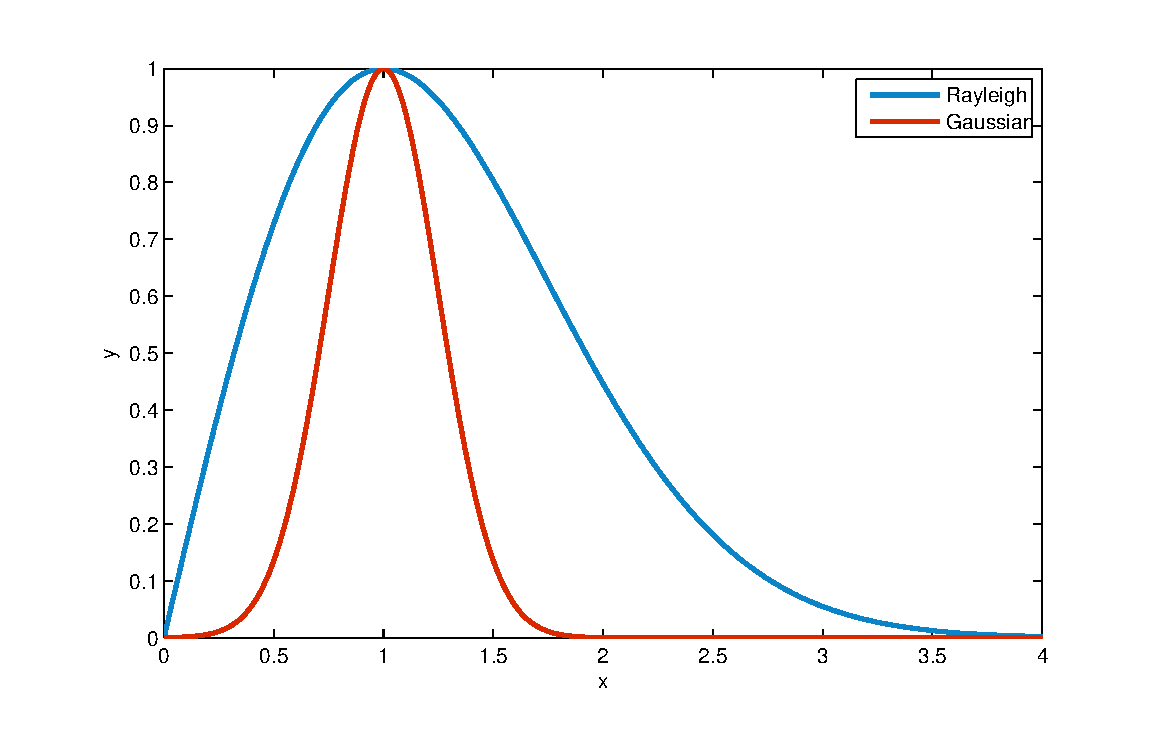
\includegraphics[width=0.7\linewidth]{3_review/figures/processing/pre-processing/noise/noisedistr.eps}
	\caption[Illustration of a Gaussian and Rayleigh distributions.]{Illustration of a Gaussian distribution ($\mu = 1, \sigma=0.25$) and a Rayleigh distribution ( $\sigma = 2$). It can be seen that the Rayleigh distribution is suffering of a bias term when compared with the Gaussian distribution.}
	\label{fig:noisedistr}
\end{figure}

%Noise filtering
\item[$-$] \textbf{\textit{Noise filtering:}} The \ac{nmr} signal measured and recorded in the k-space during an \ac{mri} acquisition is affected by noise.
This noise obeys a complex Gaussian white noise mainly due to thermal noises in the patient area \cite{Nowak1999}.
Furthermore, \ac{mri} images visualized by radiologists are in fact the magnitude images resulting from the complex Fourier transform of the k-space data.
The complex Fourier transform, being a linear and orthogonal transform, does not affect the Gaussian noise characteristics \cite{Nowak1999}.
However, the function involved in the magnitude computation is a non-linear transform (i.e., the square root of the sum of squares of real and the imaginary parts), implying that the noise distribution is no longer Gaussian; it indeed follows a Rician distribution making the denoising task harder.
Briefly, a Rician distribution can be characterized as follows: in low-\ac{si} region (low \ac{snr}), it can be approximated with a Rayleigh distribution while in high-\ac{si} region (high \ac{snr}), it is similar to a Gaussian distribution (see Fig. \ref{fig:noisedistr}) \cite{Manjon2008}.
Reviews of all denoising methods can be found in \cite{Buades2005,Mohan2014}.

Median filtering is the simplest approach used to address the denoising issue in \ac{mri} images \cite{Ozer2009,Ozer2010}.
In both studies, Ozer \textit{et al.} used a square kernel of size $5 \times 5$ pixels with the image resolutions ranging from $320 \times 256$ (cf., \ac{t2w} \ac{mri}) to $256 \times 128$ (cf., T$_2$ map, \ac{dce} and \ac{dw} \ac{mri}) and \iac{fov} ranging from 14 cm (cf, \ac{t2w} and \ac{dw} \ac{mri}) to 20 cm (cf, T$_2$ map and \ac{dce} \ac{mri}).
However, from a theoretical point of view, this simple filtering method is not well formalized to address the noise distribution in \ac{mri} images.

More complex approaches were proposed to overcome this problem.
A common method used to denoise \ac{mri} images is based on wavelet-based filtering.
This filtering exploits the sparsity property of the wavelet decomposition.
The projection of a noisy signal from the spatial-domain to the wavelet-domain implies that only few wavelet coefficients contribute to the ``signal-free noise'' while all wavelet coefficients contribute to the noise \cite{Donoho1994}.
Therefore, denoising is performed by thresholding/attenuating the insignificant wavelet coefficients to enforce the sparsity in the wavelet-domain.
Investigations focus on the strategies to perform the most adequate coefficient shrinkage method (e.g., using thresholding, singularity property or Bayesian framework) \cite{Pizurica2002}.

Ampeliotis \textit{et al.} in \cite{Ampeliotis2007,Ampeliotis2008} performed wavelet shrinkage to denoise magnitude \ac{mri} images (cf., \ac{t2w}-\ac{mri} and \ac{dce}-\ac{mri}) using thresholding techniques \cite{Mallat2008}.
However, since the wavelet transform is an orthogonal transform, the Rician distribution of the noise is preserved in the wavelet-domain.
Hence, for low \ac{snr}, the wavelet and scaling coefficients still suffer from a bias due to this specific noise distribution \cite{Nowak1999}.
 
Lopes \textit{et al.} in \cite{Lopes2011} used the filtering technique proposed by \cite{Pizurica2003} to denoise \ac{t2w}-\ac{mri} which was based on joint detection and estimation theory \cite{Pizurica2003}.
{\color{blue}
%Pizurica \textit{et al.} proposed a filtering technique based on joint detection and estimation theory \cite{Middleton1968}.
In this approach, the wavelet coefficients ``free-of-noise'' are estimated from the noisy wavelet coefficients using a \ac{map} estimate.
Furthermore, the estimator designed takes spatial context into account by including both local and global information in the prior probabilities.
The different probabilities needed by the \ac{map} are empirically estimated by using mask images representing the locations of the significant wavelet coefficients.
These mask images are computed by thresholding the detail images obtained from the wavelet decomposition.
To remove the bias from the wavelet and scaling coefficients, the squared magnitude \ac{mri} image used instead of the magnitude \ac{mri} image as proposed by \cite{Nowak1999}.
This involves changing the Rician distribution to a scaled non-central Chi-square distribution.
It implies that the wavelet coefficients are also unbiased estimators and the scaling coefficients are unbiased estimators but up to a constant $C$ as defined in Eq. \eqref{eq:nowakC} which needs to be subtracted from each scaling coefficient,

\begin{equation}
	C=2^{(J+1)}\hat{\sigma}^2 \ ,
	\label{eq:nowakC}
\end{equation}

\noindent where $J$ is the number of levels of the wavelet decomposition and $\hat{\sigma}$ is an estimate of the noise standard deviation.
}
\begin{figure}
\centering
	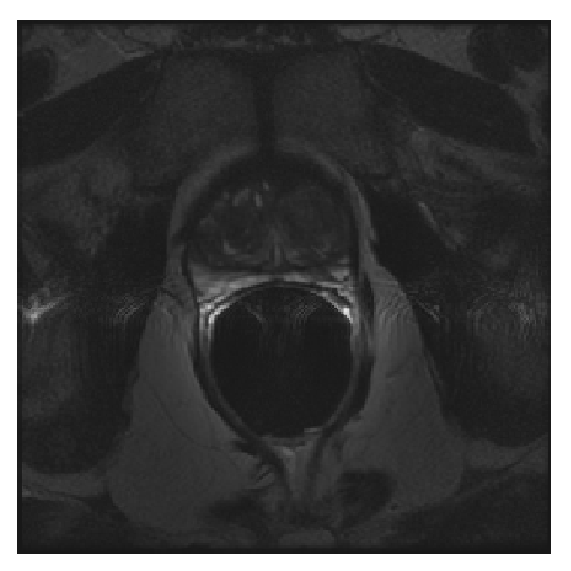
\includegraphics[width=0.3\linewidth]{3_review/figures/processing/pre-processing/bias/t2w_bias_antenna.eps}
	\caption[Inhomogeneity artefacts due to perturbation of the endorectal coil.]{Example of artefacts with high \ac{si} due to perturbation from the endorectal coil which create inhomogeneity.}
	\label{fig:bias}
\end{figure}

% Artefacts filtering
\item[$-$] \textbf{\textit{Bias correction:}} Besides being corrupted by noise, \ac{mri} images are also affected by the inhomogeneity of the \ac{mri} field commonly referred to as bias field \cite{Styner2000}.
This bias field results in a smooth variation of the \ac{si} through the image.
When an endorectal coil is used, an artefact resulting of an hyper-intense signal can be observed around the coil on the images (see Fig.~\ref{fig:bias}).

As a consequence, the \ac{si} of identical tissues varies depending on their spatial location in the image making further processes such as segmentation or registration harder \cite{Jungke1987,Vovk2007}.
A review of bias correction methods can be found in \cite{Vovk2007}.

{\color{blue}
The model of image formation is usually formalized such that:

\begin{equation}
	s(\mathbf{x}) = o(\mathbf{x})b(\mathbf{x}) + \eta(\mathbf{x}) \ ,
	\label{eq:biasmodel}
\end{equation}

\noindent where $s(\mathbf{x})$ is the corrupted \ac{si} at the pixel for the image coordinates $\mathbf{x} = \{x,y\}$, $o(\mathbf{x})$ is the ``noise-free signal'' , $b(\mathbf{x})$ is the bias field function and $\eta(\mathbf{x})$ is an additive white Gaussian noise.
%
%By using property of logarithm, the model of Eq. \eqref{eq:biasmodel} becomes additive such that:
%
%\begin{eqnarray}
%	\log s(\mathbf{x}) - \log b(\mathbf{x}) & = & \log \left( o(\mathbf{x}) + \frac{\eta(\mathbf{x})}{b(\mathbf{x})} \right) \ , \\ \nonumber
%	& = & \log \hat{o}(x) \ .
%\end{eqnarray}
%
%\noindent where $\hat{o}(\mathbf{x})$ is the signal only degraded by noise \cite{Styner2000}.

Hence, the task of bias correction involves estimating the bias function $b(\mathbf{x})$ in order to infer the ``signal-free bias'' $o(\mathbf{x})$.
% and subtract to the logarithm of the initial signal in order to obtain an estimated ``signal-free bias''.
}

Viswanath \textit{et al.}~\cite{Viswanath2009} performed bias correction on \ac{t2w}-\ac{mri} using a parametric Legendre polynomial model proposed in \cite{Styner2000} and available in the \ac{itk} library\footnote{The \ac{itk} library is available at: \texttt{http://www.itk.org/}}.

{\color{blue}
Styner \textit{et al.}~\cite{Styner2000} chose to model the bias field by using a linear combination of Legendre polynomials as:

\begin{equation}
	\hat{b}(\mathbf{x},\mathbf{p}) = \sum_{i=0}^{m-1} p_i f_i(\mathbf{x}) =  \sum_{i=0}^{l} \sum_{j=0}^{l-i} p_{ij} P_i(x) P_j(y) \ ,
	\label{eq:biascorr}
\end{equation}

\noindent where $\hat{b}$ is the bias estimation with the image coordinates $\mathbf{x} = \{x,y\}$ and the $m$ coefficients of the linear combination $\mathbf{p} = {p_{11},\dotsc,p_{ij}}$ ; $m$ can be defined as $m=(l+1)\frac{(l+2)}{2}$ where $l$ is the degree of Legendre polynomials chosen and $P_i(\cdot)$ denotes a Legendre polynomial of degree $i$.

This family of functions allows us to model the bias as a smooth inhomogeneity function across the image.
To estimate the set of parameters $\mathbf{p}$, a cost function is defined which relies on the following assumptions: (i) an image is composed of $k$ regions with $\mu_k$ being the mean \ac{si} and a variance $\sigma^{2}_{k}$ of each particular class, and (ii) each noisy pixel belongs to one of the $k$ regions with its \ac{si} value close to the class mean $\mu_k$.
Hence, the cost function is defined as:

\begin{equation}
	C(\mathbf{p}) = \sum_{\mathbf{x}} \prod_{k} \rho_k(s(\mathbf{x}) - \hat{b}(\mathbf{x},\mathbf{p}) - \mu_k) \ ,
	\label{eq:costbias}
\end{equation}

\begin{equation}
	\rho_k(x) = \frac{x^2}{x^2 + 3 \sigma_k^2} \ ,
	\label{eq:mestbias}
\end{equation}

\noindent where $\rho_k(\cdot)$ is a M-estimator allowing estimations to be less sensitive to outliers than usual square distance \cite{Li1996}.

Finally, estimation of the parameters $\mathbf{p}$ results in finding the minimum of the cost function $C(\mathbf{p})$.
This optimization was performed using the non-linear $(1+1)$ \ac{es} optimizer \cite{Styner1997}.

In a later publication, \cite{Viswanath2012} make use of the well known N3 algorithm\footnote{The N3 algorithm implementation is available at: \texttt{http://www.bic.mni.mcgill.ca/\allowbreak software/N3/}} to correct \ac{t2w}-\ac{mri} developed by \cite{Sled1998}.
To estimate the bias function, \cite{Sled1998} proposed to estimate the \acp{pdf} of the signal and bias.

Recalling Eq.~\eqref{eq:biasmodel} and taking advantage of logarithm property, it implies that this model becomes additive such that:

\begin{eqnarray}
	\log s(\mathbf{x}) & = & \log b(\mathbf{x}) + \log \left( o(\mathbf{x}) + \frac{\eta(\mathbf{x})}{b(\mathbf{x})} \right) \ , \nonumber \\
	& \approx & \log b(\mathbf{x}) + \log \hat{o}(\mathbf{x}) \ , \label{eq:logbias}
\end{eqnarray}

\noindent where $\hat{o}(\mathbf{x})$ is the signal only degraded by noise. \cite{Sled1998} shows that Eq. \eqref{eq:logbias} can be related to \acp{pdf} such that:

\begin{equation}
	S(s) = B(s) * O(s) \ ,
	\label{eq:distrbias} 
\end{equation}

\noindent where $S$, $B$ and $O$ are respectively the probability densities of $s$, $b$ and $o$.

Restoring the corrupted signal $s$ is carried out by finding the multiplicative field $b$ which maximizes the frequency content of the distribution $O$.
Sled \textit{et al.}~\cite{Sled1998} argue that a search through all possible fields $b$ and selection of the one which maximizes the high frequency content of $O$ could be carried out but results in an exhaustive search.
However, they show that the bias field distribution can be assimilated to a near Gaussian distribution.
Using this fact as \textit{a priori}, it is then possible to infer the distribution $O$ using Wiener deconvolution given $B$ and $S$ and later estimate the corresponding smooth field $b$.
}

Lv \textit{et al.}~\cite{Lv2009} corrected the inhomogeneity in \ac{t2w}-\ac{mri} images by using the method proposed in \cite{Madabhushi2006}.
In this method, the \ac{mri} images are corrected iteratively by successively detecting the image foreground via \ac{gscale} and estimating a bias field function based on a second-order polynomial model. 
{\color{blue}
First the background of the \ac{mri} image is eliminated by threholding.
The threshold value is commonly equal to the mean \ac{si} of the considered image.
Then, in the seeded region growing algorithm is applied considering every thresholded pixel as a potential seed.
However, pixels already assigned to a region will not be considered any more as seed.
As in seeded region growing algorithm \cite{Shapiro2001}, two criteria are taken into account to expand the region.
First, the region will grow using a connected-neighbourhood, initially defined by the user.
Then, the homogeneity of \ac{si} is based on a fuzzy membership function taking into account the absolute difference of the \acp{si} of two pixels.
Depending on the membership value (cf., a threshold has to be defined), the pixel considered is merged or not to the region.
Once this segmentation is performed, the largest region $R$ is used as a mask to select pixels of the original image and the mean \ac{si}, $\mu_{R}$, is computed. 
The background variation $b(\mathbf{x})$ is estimated as:

\begin{equation}
	b(\mathbf{x}) = \frac{s(\mathbf{x})}{\mu_{R}}, \ \forall \mathbf{x} \in R \ ,
	\label{eq:backest}
\end{equation}

\noindent where $s(\mathbf{x})$ is the original \ac{mri} image.

Finally, a second order polynomial $\hat{b}_{\Theta}(\mathbf{x})$ is fitted in a least-squares sense (Eq.~\eqref{eq:lsolv}),

\begin{equation}
	\hat{\Theta} = \argmin_{\Theta} | b(\mathbf{x}) - \hat{b}_{\Theta}(\mathbf{x}) |^{2}, \ \forall \mathbf{x} \in R \ .
	\label{eq:lsolv}
\end{equation}

Finally, the whole original \ac{mri} image is corrected by dividing it by the estimated bias field function $\hat{b}_{\Theta}(\mathbf{x})$.
This process is repeated until the number of pixels in the largest region $R$ does not change significantly between two iterations.
}

%SI normalization
\item[$-$] \textbf{\textit{\Ac{si} normalization/standardization:}}

As discussed in the later section, segmentation or classification tasks are usually performed by first learning from a training set of patients.
Hence, one can emphasize the desire to perform \ac{mri} examinations with a high repeatability or in other words, one would ensure to obtain similar \ac{mri} images (cf., similar \acp{si}) for patients of the same group (cf., healthy patients \textit{vs.} patients with \ac{cap}), for a similar sequence.

However, it is a known fact that variability between patients occurs during the \ac{mri} examinations even using the same scanner, protocol or sequence parameters \cite{Nyul1999}.
Hence, the aim of normalization or standardization of the \ac{mri} data is to remove the variability between patients and enforce the repeatability of the \ac{mri} examinations.
Approaches used to standardize \ac{mri} images can be either categorized as statistical-based standardization or organ \ac{si}-based standardization. 

Artan \textit{et al.}~\cite{Artan2009,Artan2010} as well as Ozer \textit{et al.}~\cite{Ozer2009,Ozer2010} standardized \ac{t2w}, \ac{dce} and \ac{dw} \ac{mri} images by computing the \textit{standard score} (also called \textit{z-score}) of the pixels of the \ac{pz} as:

\begin{equation}
	I_s(\mathbf{x}) = \frac{ I_r(\mathbf{x}) - \mu_{pz}}{\sigma_{pz}}, \ \forall \mathbf{x} \in \text{PZ} \ ,
	\label{eq:meansta}
\end{equation}

\noindent where $I_s(\mathbf{x})$ is the standardized \ac{si} with the image coordinates $\mathbf{x} = \{x,y\}$, $I_r(\mathbf{x})$ is the raw \ac{si}, $mu_{pz}$ is the mean-\ac{si} of the \ac{pz} and $\sigma_{pz}$ is the \ac{si} standard deviation in the \ac{pz}.
This transformation enforces the image \ac{pdf} to have a zero mean and a unit standard deviation.

In a similar way, Liu \textit{et al.}~\cite{Liu2013} normalized \ac{t2w}-\ac{mri} by making use of the median and interquartile range for all the pixels.

Lv \textit{et al.}~\cite{Lv2009} scaled the \ac{si} of \ac{t2w}-\ac{mri} images using the method proposed in \cite{Nyul2000} based on \ac{pdf} matching.
This approach is based on the assumption that \ac{mri} images from the same sequence should share the same \ac{pdf} appearance.
Hence, one can approach this issue by transforming and matching the \acp{pdf} using some statistical landmarks such as median and different quantiles.
Using a training set, these statistical landmarks are extracted for $N$ training images as for instance for the minimum, the $25^{\text{th}}$ quantile, the median, the $75^{\text{th}}$ quantile and the maximum:

\begin{eqnarray}	
	\Phi_{0} & = & \{ \phi_{0}^{1}, \phi_{0}^{2}, \cdots, \phi_{0}^{N} \} \ , \nonumber \\
	\Phi_{25} & = & \{ \phi_{25}^{1}, \phi_{25}^{2}, \cdots, \phi_{25}^{N} \} \ , \nonumber \\
	\Phi_{50} & = & \{ \phi_{50}^{1}, \phi_{50}^{2}, \cdots, \phi_{50}^{N} \} \ ,  \label{eq:quantileStd} \\
	\Phi_{75} & = & \{ \phi_{75}^{1}, \phi_{75}^{2}, \cdots, \phi_{75}^{N} \} \ , \nonumber \\
	\Phi_{100} & = & \{ \phi_{100}^{1}, \phi_{100}^{2}, \cdots, \phi_{100}^{N} \} \ , \nonumber
\end{eqnarray}

\noindent where $\phi_{n^\text{th}}^{i^{\text{th}}}$ is the $n^{\text{th}}$ quantile of the $i^{\text{th}}$ training image.

\begin{figure}
	\centering
	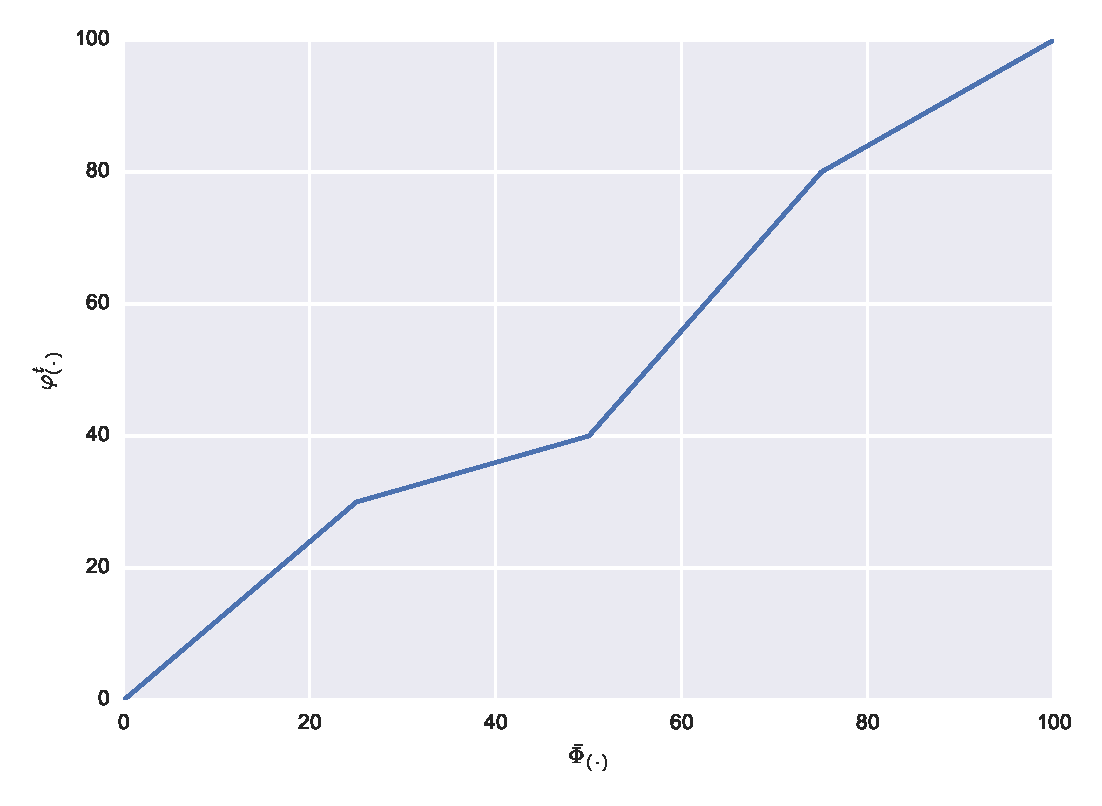
\includegraphics[width=0.7\linewidth]{3_review/figures/processing/pre-processing/normalization/linear_transform_parts.eps}
	\caption{Example of linear mapping by parts as proposed by \cite{Nyul2000}.}
	\label{fig:imnorm}
\end{figure}

Then, the mean of each quantile $\{ \bar{\Phi}_{0}, \bar{\Phi}_{25}, \bar{\Phi}_{50}, \bar{\Phi}_{75}, \bar{\Phi}_{100} \}$ is also calculated.
Once this training stage is performed, a linear transformation by parts $\mathcal{T}(\cdot)$ can be computed (Eq.~\eqref{eq:linearMap}) for each test image $t$ by mapping each statistical landmark $\varphi_{(cdot)}̂^{t}$ of this image with the pre-learned statistical landmarks $\bar{\Phi}_{(\cdot)}$.
This linear mapping is also depicted in Fig.~\ref{fig:imnorm}.

\begin{equation}
\small
\mathcal{T}(s(\mathbf{x})) =
  \begin{cases}
    \lceil \bar{\Phi}_{0}+( s(\mathbf{x}) - \varphi_{0}^{t} ) \left( \frac{\bar{\Phi}_{25} - \bar{\Phi}_{0}}{\varphi_{25}^{t} - \varphi_{0}^{t}} \right) \rceil \ , & \text{if $\varphi_{0}^{t} \leq s(\mathbf{x})<\varphi_{25}^{t})$} \ , \\
    \lceil \bar{\Phi}_{25}+( s(\mathbf{x}) - \varphi_{25}^{t} ) \left( \frac{\bar{\Phi}_{50} - \bar{\Phi}_{25}}{\varphi_{50}^{t} - \varphi_{25}^{t}} \right) \rceil \ , & \text{if $\varphi_{25}^{t} \leq s(\mathbf{x})<\varphi_{50}^{t})$} \ , \\
    \lceil \bar{\Phi}_{50}+( s(\mathbf{x}) - \varphi_{50}^{t} ) \left( \frac{\bar{\Phi}_{75} - \bar{\Phi}_{50}}{\varphi_{75}^{t} - \varphi_{50}^{t}} \right) \rceil \ , & \text{if $\varphi_{50}^{t} \leq s(\mathbf{x})<\varphi_{75}^{t})$} \ , \\
    \lceil \bar{\Phi}_{75}+( s(\mathbf{x}) - \varphi_{75}^{t} ) \left( \frac{\bar{\Phi}_{100} - \bar{\Phi}_{75}}{\varphi_{100}^{t} - \varphi_{75}^{t}} \right) \rceil \ , & \text{if $\varphi_{75}^{t} \leq s(\mathbf{x})\leq \varphi_{100}^{t})$} \ ,
  \end{cases}
  \label{eq:linearMap}
\end{equation}

Viswanath \textit{et al.}~\cite{Viswanath2009,Viswanath2011,Viswanath2012} use a variant of this previous approach presented in \cite{Madabhushi2006a} aiming to standardize the \ac{t2w}-\ac{mri} images.Instead of computing the \ac{pdf} of an entire image, a pre-segmentation of the foreground is carried out via \ac{gscale} which was discussed in the bias correction section.
Once the foreground is detected, the largest region is extracted and the same process than previously mentioned (see Eq.~\eqref{eq:linearMap}) takes place in order to align \acp{pdf} of the foreground of the \ac{mri} images.

\begin{figure}
\centering
	\hspace*{\fill}
	\subfigure[Illustration and location of the bladder on a \ac{t2w}-\ac{mri} image acquired with a 3.0 Tesla \ac{mri} scanner]{\label{subfig:bladder} 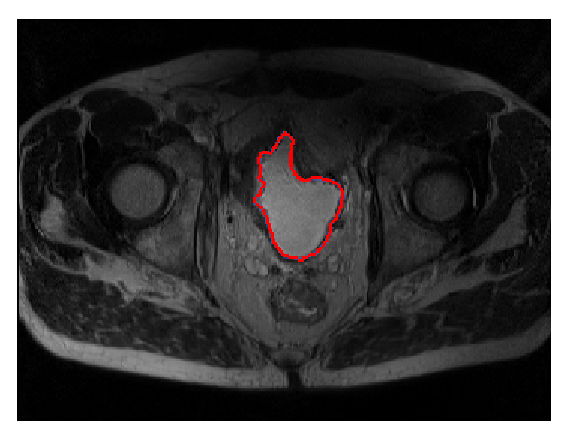
\includegraphics[width=0.3\linewidth]{3_review/figures/processing/pre-processing/niaf/t2w_bladder.eps}} \hfill
	\subfigure[Illustration and location of the femoral arteries on a \ac{t1w}-\ac{mri} image acquired with a 3.0 Tesla \ac{mri} scanner]{\label{subfig:arteries} 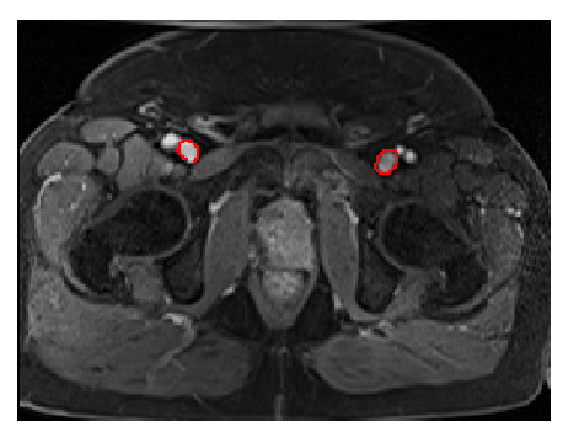
\includegraphics[width=0.3\linewidth]{3_review/figures/processing/pre-processing/niaf/t1w_arteries.eps}}
	\hspace*{\fill}
	\caption{Illustration of the two organs used by \cite{Niaf2011,Niaf2012} to normalize \ac{t2w} and \ac{t1w} \ac{mri} images.}
	\label{fig:niaf}
\end{figure}

The methods described above were statistical-based methods.
However, the standardization problem can be tackled by normalizing the MRI images using the \ac{si} of some known organs present in these images. 
Niaf \textit{et al.}~\cite{Niaf2011,Niaf2012} normalized \ac{t2w}-\ac{mri} images by dividing the original \ac{si} of the images by the mean \ac{si} of the bladder (see Fig.~\ref{subfig:bladder}).
Likewise, \cite{Niaf2011} standardized the \ac{t1w}-\ac{mri} images using the \ac{aif}.
They computed the \ac{aif} by taking the mean of the \ac{si} in the most enhanced part of the common femoral arteries (see Fig. \ref{subfig:arteries}) as proposed in \cite{Wiart2007}.

\end{enumerate}


Presented in Sect.~\ref{subsec:chp2:imaging:mrsi}, \ac{mrsi} is a modality related to a one dimensional signal.
Hence, specific pre-processing steps for this type of signals have been applied instead of standard signal processing methods.

\setenumerate{listparindent=\parindent,itemsep=10px}
\setlist{noitemsep}
\begin{enumerate}[leftmargin=*]

\begin{figure}
	\centering
	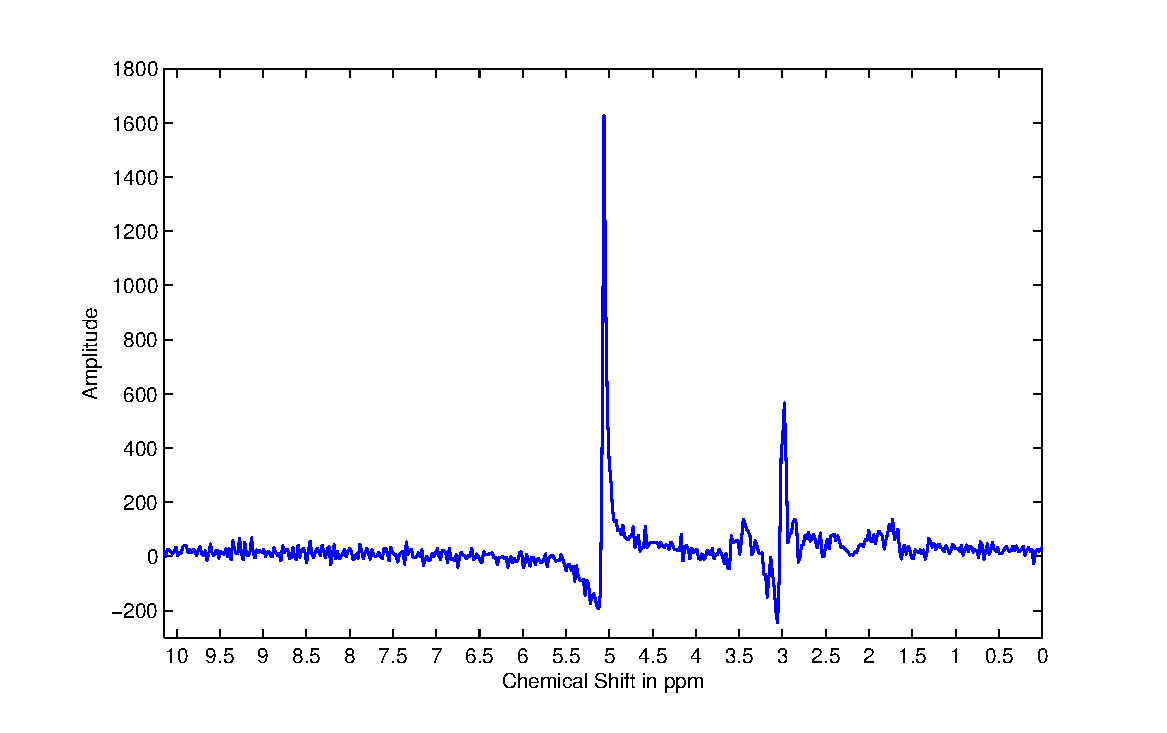
\includegraphics[width=0.7\linewidth]{3_review/figures/processing/pre-processing/phase/phase.eps}
	\caption[Illustration of phase malignant in an \ac{mrsi} spectra.]{Illustration of phase misalignment in an \ac{mrsi} spectra acquire with a 3.0 Tesla \ac{mrsi} scanner. Note the distortion of the signal specially visible for the water and citrate peaks.}
	\label{fig:phase}
\end{figure}

	\item[$-$] \textbf{\textit{Phase correction:}} \ac{mrsi} data acquired suffer from zero-order and first-order phase misalignments as shown in Fig.~\ref{fig:phase} \cite{Chen2002,Osorio-Garcia2012}. 
Parfait \textit{et al.}~\cite{Parfait2012} used a method proposed in \cite{Chen2002} where the phase of \ac{mrsi} signal is corrected based on entropy minimization in the frequency domain.
The corrected \ac{mrsi} signal $o(\xi)$ can be expressed as:

\begin{eqnarray}
	\Re(o(\xi)) & = & \Re(s(\xi))\cos(\Phi(\xi)) - \Im(\xi)\sin(\Phi(\xi)) \ , \nonumber  \\
	\Im(o(\xi)) & = & \Im(s(\xi))\cos(\Phi(\xi)) + \Re(\xi)\sin(\Phi(\xi)) \ , \nonumber \\
	\Phi(\xi) & = & \phi_0 + \phi_1 \frac{\xi}{N} \ , \label{eq:mrsiphcorr}
\end{eqnarray}

\noindent where $\Re(\cdot)$ and $\Im(\cdot)$ are the real and imaginary part of the complex signal respectively, $s(\xi)$ is the corrupted \ac{mrsi} signal, $\phi_0$ and $\phi_1$ are the zero-order and first-order phase correction terms respectively and $N$ is the total number of samples of the \ac{mrsi} signal.

Chen \textit{et al.}~\cite{Chen2002} tackled this problem using an optimization framework where $\phi_0$ and $\phi_1$ had to be inferred.
Hence, the simplex Nelder-Mead optimization method was used to minimize the following cost function based on the \textit{Shannon entropy} formulation:

\begin{equation}
	\hat{\Phi} = \argmin_{\Phi} \left[ - \sum \Re(s'(\xi)) \ln \Re(s'(\xi)) + \lambda \|\Re(s(\xi))\|_2 \right] \ ,
	\label{eq:phcost}
\end{equation}

\noindent where $s'(\xi)$ is the first derivative of the corrupted signal $s(\xi)$ and $\lambda$ is a regularization parameter.
Once the best parameter $\Phi$ is obtained, the \ac{mrsi} signal is corrected using Eq.~\eqref{eq:mrsiphcorr}.

\begin{figure}
\centering
	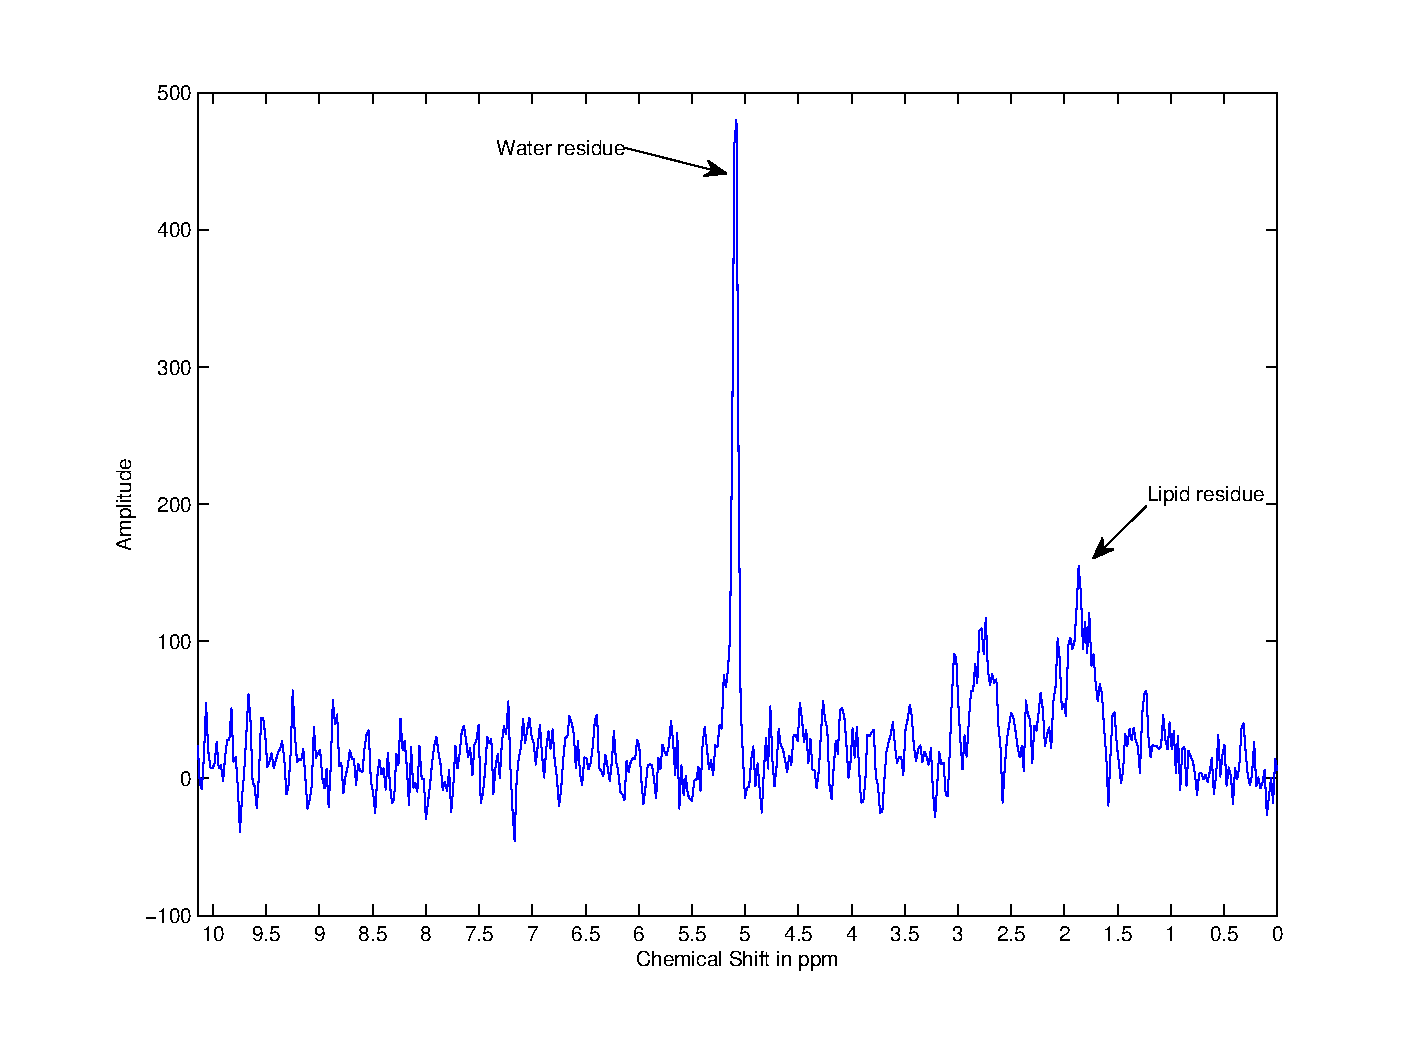
\includegraphics[width=0.7\linewidth]{3_review/figures/processing/pre-processing/water/water_fat.eps}
	\caption[Illustration of water and fat residues in \ac{mrsi} signal after supression during acquisition.]{Illustration of the residues of water and fat even after their suppression during the acquisition protocol. The acquisition was carried out with a 3.0 Tesla \ac{mri}.}
	\label{fig:waterfat}
\end{figure}

	\item[$-$] \textbf{\textit{Water and lipid residuals filtering:}} The water and lipid metabolites occur in much higher concentrations the metabolites of interests (cf., choline, creatine and citrate) \cite{Zhu2010,Osorio-Garcia2012}.
Fortunately, specific \ac{mrsi} sequences were developed in order to suppress water and lipid metabolites using pre-saturation techniques \cite{Zhu2010}.
However, these techniques do not perfectly remove water and lipids peaks and some residuals are still present in the \ac{mrsi} spectra as shown in Fig.~\ref{fig:waterfat}.
Therefore, different post-processing methods have been proposed to enhance the quality of the \ac{mrsi} spectra by removing these residuals.
For instance, Kelm \textit{et al.}~\cite{Kelm2007} used the well known HSVD algorithm proposed by \cite{Pijnappel1992} which models the \ac{mrsi} signal by a sum of exponentially damped sinusoids in the time domain (see Eq.~\eqref{eq:fidsig}).
%In the time domain, a \ac{mrsi} signal $s(t)$ is modelled by a sum of $K$ exponentially damped sinusoids such that:

\begin{equation}
	s(t) = \sum_{k=1}^{K} a_{k}\exp(i \phi_k) \exp( -d_{k} + i 2 \pi f_{k} ) t + \eta(t) \ ,
	\label{eq:fidsig}
\end{equation}

\noindent where $a_k$ is the amplitude proportional to the metabolite concentration with a resonance frequency $f_{k}$, $d_k$ represents the damping factor of the exponential, $\phi_k$ is the first-order phase and $\eta(t)$ is a complex white noise. 

Pijnappel \textit{et al.}~\cite{Pijnappel1992} showed that the ``noise-free signal'' can be found using the \ac{svd} decomposition.
First the noisy signal is reorganized inside a Hankel matrix $H$.
It can be shown that if the signal considered would be a ``noise-free signal'', the rank of $H$ would be equal to rank $K$.
However, due to the presence of noise, $H$ is in fact a full rank matrix.
Thus, to recover the ``noise-free signal'', the rank of $H$ can be truncated to $K$ using its \ac{svd} decomposition.
Hence, knowing the cut off frequencies of water (cf., 4.7 ppm) and lipid (cf., 2.2 ppm) metabolites, their corresponding peaks can be reconstructed and subtracted from the original signal \cite{Laudadio2002}.
	
	\item[$-$] \textbf{\textit{Baseline correction:}} Sometimes, the problem discussed in the above section regarding the lipid molecules is not addressed simultaneously with water residuals suppression.
Lipids and macromolecules are known to affect the baseline of the \ac{mrsi} spectra.
They could cause errors during further fitting processes aiming to quantify the metabolites, especially regarding the citrate metabolite.
	
Parfait \textit{et al.}~\cite{Parfait2012} made the comparison of two different methods to detect the baseline and correct the \ac{mrsi} spectra which are based on \cite{Lieber2003,Devos2004}. 
Lieber \textit{et al.}~\cite{Lieber2003} addressed the problem of baseline detection in the frequency domain by fitting a low degree  polynomial whereas Parfait \textit{et al.}~\cite{Parfait2012} modified this algorithm by convolvinga Gaussian kernel to smooth the \ac{mrsi} signal instead of fitting a polynomial function.
{\color{red} \textbf{Check the tex file to see the commented area pre-processing.tex}}
%% of low degree $p(x)$ (e.g., second or third degree) to the \ac{mrsi} signal $s(x)$ in a least-squares sense.
%% Then, the values of the fitted polynomial are re-assigned as:

%% \begin{equation}
%% 	p_f(x) = 
%% 	\begin{cases}
%% 		p(x) \ , & \text{if $p(x) \leq s(x)$} \ , \\
%% 		s(x) \ , & \text{if $p(x) > s(x)$} \ . \\
%% 	\end{cases}
%% 	\label{eq:lieber}
%% \end{equation}

%% Finally, this procedure of fitting and re-assignment is iteratively repeated on $p_f(x)$ until a stopping criterion is reached. The final polynomial function can be subtracted from the original signal s(x) to correct it.

%% \cite{Parfait2012} modified this algorithm by convolving a Gaussian kernel to smooth the \ac{mrsi} signal instead of fitting a polynomial function, keeping the rest of the algorithm identical. 
Unlike in \cite{Lieber2003}, Devos \textit{et al.}~\cite{Devos2004} proposed to correct the baseline in the time domain by multiplying the \ac{mrsi} signal by a decreasing exponential function as:
\begin{equation}
	c(t) = \exp (- \beta t) \ ,
	\label{eq:devos}
\end{equation}

\noindent Having a typical value for $\beta$ of 0.15.
However, Parfait \textit{et al.}~\cite{Parfait2012} concluded that the method proposed in \cite{Lieber2003} outperformed the one in \cite{Devos2004}.

In the contemporary work of Tiwari \textit{et al.}~\cite{Tiwari2012}, the authors detected the baseline using a local non-linear fitting method avoiding regions with significant peaks which were detected using a experimentally parametrised signal-to-noise ratio (i.e. a value larger than 5 dB).


\begin{figure}
\centering
	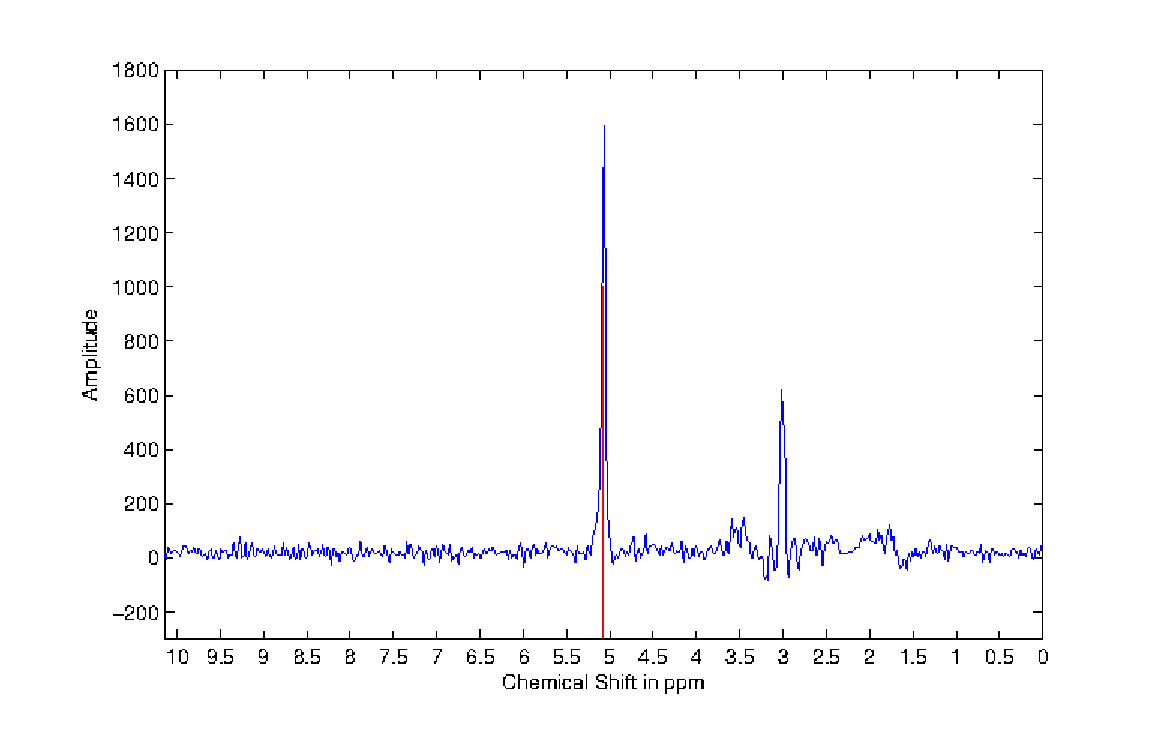
\includegraphics[width=0.7\linewidth]{3_review/figures/processing/pre-processing/frequency/frequency.eps}
	\caption[Illustration of frequency misalignment in an \ac{mrsi} spectra.]{Illustration of frequency misalignment in an \ac{mrsi} spectra acquired with a 3.0 Tesla \ac{mrsi} scanner. The water peak is known to be aligned at 4.65 ppm. However, it can be seen that the peak on this spectra is aligned at around 5.1 ppm.}
	\label{fig:frequency}
\end{figure}

	\item[$-$] \textbf{\textit{Frequency alignment:}} Due to variations of the experimental conditions, a frequency shift can be observed in the \ac{mrsi} spectra \cite{Chen2002,Osorio-Garcia2012} as shown in Fig.~\ref{fig:frequency}.
	
Tiwari \textit{et al.}~\cite{Tiwari2012} corrected the frequency shift by first detecting known metabolite peaks such as choline, creatine and citrate.
The frequency shift is corrected by minimizing the frequency error between the experimental and theoretical values of each of these peaks.

	\item[$-$] \textbf{\textit{Normalization:}} Due to variations of the experimental conditions, the \ac{mrsi} signal may also vary between patients.
Parfait \textit{et al.}~\cite{Parfait2012} as in \cite{Devos2004} compared two methods to normalize \ac{mrsi} signal.
In each method, the original \ac{mrsi} spectra is divided by a normalization factor, similar to the intensity normalization described earlier.  
The first approach to obtain the normalization factor is based on an estimation of the water concentration.
It is required to have an additional \ac{mrsi} sequence where the water metabolites are unsuppressed.
Using this sequence, an estimation of the water concentration can be performed using the previously reported HSVD algorithm.
The second approach to normalization is based on using the L$_2$ norm of the \ac{mrsi} spectra $\|s(\xi)\|_2$. 
It should be noted that both \cite{Parfait2012} and \cite{Devos2004} concluded that the L$_2$ normalization was more efficient in their framework.
 
\end{enumerate}


\begin{table}
	\caption{Overview of the pre-processing methods used in \ac{cad} systems.}
	\small
	%\renewcommand{\arraystretch}{1.5}
	\begin{tabular}{p{.65\linewidth} p{.25\linewidth}}
		\hline \\ [-1.5ex]
		\textbf{Pre-processing operations} & \textbf{References} \\ \\ [-1.5ex]
		\hline \\ [-1.5ex]
		\textit{\ac{mri} pre-processing:} & \\ \\ [-1.5ex]
		\quad Noise filtering: &  \\
		\quad \quad Median filtering & $[$20-21$]$  \\
		\quad \quad Wavelet-based filtering & $[$1-2,14$]$ \\ \\ [-1.5ex]
		\quad Bias correction: & \\
		\quad \quad Parametric methods & $[$15-35$]$ \\
		\quad \quad Non-parametric methods & $[$36$]$ \\ \\ [-1.5ex]
		\quad Standardization: & \\
		\quad \quad Statistical-based normalization: & $[$3-4,15,20-21,35,37$]$ \\
		\quad \quad Organ \ac{si}-based normalization & $[$18-19$]$ \\ \\ [-1.5ex]
		\textit{\ac{mrsi} pre-processing:} & \\ \\ [-1.5ex]
		\quad Phase correction & $[$22$]$ \\
		\quad Water and lipid residuals filtering & $[$8$]$ \\
		\quad Baseline correction & $[$22,31$]$ \\
		\quad Frequency alignment & $[$31$]$ \\
		\quad Normalization & $[$22$]$ \\ \\ [-1.5ex]
		\hline
	\end{tabular}
\label{tab:summary-preproc}
\end{table}

\subsection{Segmentation}\label{subsec:chp3:img-reg:seg}
The segmentation task consists in delineating the prostate boundaries in the \ac{mri} and is of particular importance for focusing the posterior processing on the organ of interest~\cite{Ghose2012}. 
In this section, only the segmentation methods used in \ac{cad} for \ac{cap} are presented.
An exhaustive review of prostate segmentation methods in \ac{mri} is available in~\cite{Ghose2012}.

%% \setenumerate{listparindent=\parindent,itemsep=10px}
%% \setlist{noitemsep}
%% \begin{enumerate}[leftmargin=*]

%\item[$-$] \textbf{\textit{Manual segmentation:}} 
\paragraph{Manual segmentation}
To highlight the importance of prostate segmentation task in \ac{cad} systems, it is interesting to note the large number of studies which manually segment the prostate organs~\cite{Artan2009,Artan2010,Matulewicz2013,Niaf2011,Niaf2012,Ozer2009,Ozer2010,Puech2009,Vos2008,Vos2008a,trigui2016classification,trigui2017automatic,lehaire2014computer}.
In all the cases, the boundaries of the prostate gland are manually defined in order to limit further processing to only this area.
This approach ensures the right delineation of the organ; nevertheless this procedure is highly time consuming and should be performed by a radiologist.

%\item[$-$] \textbf{\textit{Region-based segmentation:}} 
\paragraph{Region-based segmentation}
\citeauthor{Litjens2012} used a multi-atlas-based segmentation using multi-modal images --- i.e., \ac{t2w}-\ac{mri} and \ac{adc} map --- to segment the prostate with an additional pattern recognition method to differentiate \ac{cg} and \ac{pz}~\cite{Litjens2012}, as proposed in~\cite{Litjens2012a}.
This method consists in three different steps: (i) the registration between each atlas and the multi-modal images, (ii) the atlas selection, and finally (iii) the classification of the prostate voxels into either \ac{cg} or \ac{pz} classes.
Each atlas and the \ac{mri} images are registered two successive registrations: a rigid registration to roughly align the atlases and the \ac{mri} images followed by an elastic registration using a B-spline transformation.
The cost function driving the registration is defined as the weighted sum of the \ac{mi} of both \ac{t2w}-\ac{mri} and \ac{adc} map.
The final atlas is selected using either a majority voting or the \ac{staple} approach~\cite{Warfield2004}.
Subsequently, each voxel within the prostate are classified either as \ac{cg} or \ac{pz} using a \ac{lda} classifier.
Three types of feature are considered to characterized the voxels: (i) anatomy, (ii) intensity, and (iii) texture.
The relative position and the relative distance from the voxel to the border of the prostate encode the anatomical information.
The intensity features consist in the intensity of the voxel in the \ac{adc} coefficient and the T$_2$ map.
The texture features are composed of 5 different features: homogeneity, correlation~\cite{Amadasun1989}, entropy, texture strength~\cite{Li2005a}, and \ac{lbp}~\cite{Ojala1996}.
Finally, the final segmentation is obtained by removing artifacts and smoothing the contour between the zones using the \ac{tps}~\cite{Bookstein1989}.

\citeauthor{Litjens2014} used an almost identical algorithm in~\cite{Litjens2014}, initially proposed for the PROMISE12 challenge~\cite{Litjens2014a}.
Their segmentation method is also based on multi-atlas multi-modal images, but the SIMPLE method~\cite{langerak2010label} is used instead, to combine labels after the registration of the different atlas to obtain the final segmentation.
 
Finally, \citeauthor{rampun2016computerb} recurrently used a method to segment the \ac{pz}~\cite{rampun2015classifying,rampun2015computer,rampun2016computer,rampun2016computerb,rampun2016quantitative}, which is proposed in~\cite{rampun2014detection}.
The \ac{pz} is modelled using a quadratic function driven by the centre of the prostate, the left-most, and the right-most coordinates of the prostate boundaries.

%\item[$-$] \textbf{\textit{Model-based segmentation:}} 
\paragraph{Model-based segmentation}
\citeauthor{Viswanath2009} in~\cite{Viswanath2008a,Viswanath2009} used the \ac{mantra} method as proposed by \citeauthor{Toth2008}.
\ac{mantra}~\cite{Toth2008} is closely related to the \ac{asm} from~\cite{Cootes1995}.
This algorithm consists of two stages: (i) a training stage where a shape and an appearance model are generated and (ii) the actual segmentation based on the learned model. 
For the training stage, a set of landmarks is defined and the shape model is generated as in the original \ac{asm} method~\cite{Cootes1995}.
Then, to model the appearance, a set of $K$ texture images $\{I_1,I_2,\cdots,I_k\}$ based on first and second order statistical texture features is computed.
For a given landmark $l$ with its given neighbourhood $\mathcal{N}(l)$, its feature matrix extracted is expressed as:

\begin{equation}
  f_l = \{ I_1(\mathcal{N}(l)), I_2(\mathcal{N}(l)), \cdots, I_k(\mathcal{N}(l)) \} \ ,
  \label{eq:mantra1}
\end{equation}

\noindent where $I_k(\mathcal{N}(l))$ represents a feature vector obtained by sampling the $k^{\text{th}}$ texture map using the neighbourhood $\mathcal{N}(l)$.
Therefore, multiple landmarks are generated followed by a decomposition using \ac{pca}~\cite{Pearson1901} to learn the appearance variations as in \ac{asm}.

For the segmentation stage, the mean shape learned previously is initialized in the test image.
The same associated texture images as in the training stage are computed.
For each landmark $l$, a neighbourhood of patches are used to sample the texture images and a reconstruction is obtained using the appearance model previously trained.
The new landmark location will be defined as the position where the \ac{mi} is maximal between the reconstructed and original values.
This scheme is performed in a multi-resolution manner as in \cite{Cootes1995}.

Subsequently, \citeauthor{Viswanath2012} in~\cite{Viswanath2012}, used the \ac{weritas} method also proposed in~\citeauthor{Toth2009}.
Similarly to \ac{mantra}, \ac{weritas} is also based on the \ac{asm} formulation~\cite{Toth2009}.
%As with the \ac{mantra} method, \ac{weritas} is based on the \ac{asm} formulation.
%In fact it is very close to the \ac{mantra} itself. 
%The same texture features are used to construct the appearance models, but instead of using \ac{mi} between the landmarks and neighbour patches for adapting the landmark positions, it defines a metric based on the Mahalanobis distance.
They differ in the last stage of the algorithm in which the Mahalanobis distance is used instead of the \ac{mi} metric, to adapt the positions of new landmarks.
In the training stage, the Mahalanobis distance is computed between landmarks and neighbour patches for each of the features.
Subsequently, a new metric is proposed as a linear weighted combination of those Mahalanobis distances which maximizes the correlation with the Euclidean distance between the patches and the true landmarks.
In the segmentation step, this metric is then computed between the initialized landmarks and neighbouring patches in order to update landmark positions, in a similar fashion to other \ac{acm} models.

\citeauthor{Litjens2011} as well as \citeauthor{Vos2012} used an approach proposed in~\cite{Huisman2010} in which the bladder, the prostate, and the rectum are segmented~\cite{Litjens2011,Vos2012}.
The segmentation task is performed as an optimization problem taking 3 parameters into account linked to organ characteristics such as: (i) the shape (i.e., an ellipse), (ii) the location, and (iii) the respective angles between them.
Furthermore, \citeauthor{Litjens2011} used only the \ac{adc} map to encode the appearance~\cite{Litjens2011} whereas \citeauthor{Vos2012} used both \ac{adc} and T$_2$ maps~\cite{Vos2012}.
The cost function, defined as the sum of the deviations, is minimized using a quasi-Newton optimizer.
This rough segmentation is then used inside a Bayesian framework to refine the segmentation.

\citeauthor{giannini2015fully} segmented the prostate with a multi-Otsu thresholding~\cite{otsu1975threshold} in \ac{adc} images~\cite{giannini2015fully}.
Further morphological operations are applied to improve the segmentation.

Only the work of \citeauthor{Tiwari2009} used the \ac{mrsi} modality to segment the prostate~\cite{Tiwari2009}.
The prostate is segmented based on an unsupervised hierarchical spectral clustering.
First, each \ac{mrsi} spectrum is projected into a lower-dimensional space using graph embedding~\cite{Shi2000}.
To proceed, a similarity matrix $W$ is computed using a Gaussian similarity measure from Euclidean distance~\cite{Belkin2001} such that:

\begin{equation}
	W(\mathbf{x},\mathbf{y}) =
	\begin{cases}	
	 	\exp \left( \frac{\| s(\mathbf{x}) - s(\mathbf{y}) \|_2^2}{\sigma^2} \right) \ , & \text{if } \| \mathbf{x} - \mathbf{y} \|_2 < \epsilon \ , \\
	 	0 \ , & \text{if } \| \mathbf{x} - \mathbf{y} \|_2 > \epsilon \ .
	 \end{cases}
	\label{eq:ge1}
\end{equation}

\noindent where $s(\mathbf{x})$ and $s(\mathbf{y})$ are the \ac{mrsi} spectra for the voxels $\mathbf{x}$ and $\mathbf{y}$, respectively, $\sigma$ is the standard deviation of the Gaussian similarity measure, and $\epsilon$ is the parameter to defined an $\epsilon$-neighbourhood.

The projection can be performed as a generalized eigenvector problem such that:
\begin{eqnarray}
  Lu & = & \lambda D u \ , \nonumber \\
  D(\mathbf{x},\mathbf{x}) & = & \sum_{\mathbf{y}} W(\mathbf{x},\mathbf{y}) \ , \label{eq:ge2} \\
  L & = & D-W \ , \nonumber
\end{eqnarray}

\noindent where $D$ is the diagonal weight matrix, $L$ is the Laplacian matrix, $\lambda$ and $u$ represent the eigenvalues and eigenvectors.
Once that the \ac{mrsi} spectra are projected into the lower-dimensional space, a replicate k-means clustering method is used to define 2 clusters.
Subsequently, the data corresponding to the largest cluster is assumed to belong to the non-prostate voxels and thus these voxels are eliminated from the processing.
The full procedure is repeated until the total number of voxels left is inferior to a given threshold experimentally set.

%\end{enumerate}

\subsubsection{Summary}

The segmentation used in \ac{cad} system for the detection of \ac{cap} are summarized in \ac{tab}~\ref{tab:summary-seg}.

\begin{table}
  \caption{Overview of the segmentation methods used in \ac{cad} systems.}
  \scriptsize
  \centering
  \begin{tabular}{l r}
    \toprule
    \textbf{Segmentation methods} & \textbf{References} \\
    \midrule
    \textbf{\ac{mri}-based segmentation:} & \\ \\ [-1.5ex]
    \quad Manual segmentation & \cite{Artan2009,Artan2010,Matulewicz2013,Niaf2011,Niaf2012,Ozer2009,Ozer2010,Puech2009,Vos2008,Vos2008a,Vos2010,Vos2012,trigui2016classification,trigui2017automatic,lehaire2014computer} \\
    \quad Region-based segmentation & \cite{Litjens2012,Litjens2014,rampun2015classifying,rampun2015computer,rampun2016computer,rampun2016computerb,rampun2016quantitative} \\
    \quad Model-based segmentation & \cite{Litjens2011,Viswanath2008a,Viswanath2009,Viswanath2011,Vos2012,giannini2015fully} \\ \\ [-1.5ex]
    \textbf{\ac{mrsi}-based segmentation:} & \\ \\ [-1.5ex]
    \quad Clustering & \cite{Tiwari2009} \\
    \bottomrule
  \end{tabular}
\label{tab:summary-seg}
\end{table}

\subsection{Registration}\label{subsec:chp3:img-reg:reg}
\input{3_review/fig-reg-framework.tex}

Image registration plays a vital role in \ac{cad} systems using \ac{mpmri} images.
As it will be discussed in \acs{sec}\,\ref{sec:chp3:img-clas}, the features detected in each modality are grouped depending of their spatial location, requiring a perfect alignment of the \ac{mpmri} ahead of the classification.

Image registration is the procedure consisting of aligning an unregistered image --- also called moving image --- into a template image --- also called fixed image --- via a geometric transformation.
This problem is usually addressed as depicted in \ac{fig}\,\ref{fig:frareg}.
An iterative procedure takes place to infer the geometric transformation, parametric or non-parametric, via an optimizer which maximizes the similarity between the two images.
In the following, a review of the different components of a typical registration framework: transformation model, similarity metric, optimizer, and interpolation are presented.
To conclude a summary is given focusing on the registration approaches applied in \ac{cad} for \ac{cap} systems.
Exhaustive reviews covering all registration methods in computer science and medical fields can be found in~\cite{Maintz1998,Zitova2003}.

%From Sect. \ref{subsubsec:geotra} to \ref{subsubsec:int}, we individually review the different components of a typical registration framework (Fig \ref{fig:frareg}).
%Section \ref{subsubsec:regrev} will summarize the combinations of these components especially for the frameworks used in \ac{cad} systems. 

%% \setenumerate{listparindent=\parindent,itemsep=10px}
%% \setlist{noitemsep}
%% \begin{enumerate}[leftmargin=*]

%\item[$-$] \textbf{\textit{Geometric transformation models:}} 
\paragraph{Geometric transformation models}
%% From all \ac{cad} for \ac{cap} systems reviewed, only parametric transformation models have been used, mainly based on affine and elastic transformation.
%% Affine transformations provide dgrees of freedom managaing rotations and translation as with the rigid transformations but also shearing and scaling.
As previously mentioned, the registration process is equivalent to find a geometric transformation which minimizes the difference between two images.
From all \ac{cad} systems reviewed, only parametric methods have been implemented.
Three different groups of parametric transformation models have been used --- i.e., rigid, affine, and elastic --- each of them characterized by a specific degree of freedom.

The simplest transformation used in terms of degree of freedom is usually referred to as rigid transformation.
This type of transformation is only composed of a rotation and a translation.
Therefore, for the 2D case where $\mathbf{x} = (x,y) \in \mathbb{R}^2$, a rigid transformation $\mathcal{T}_R$ is formalized as:

\begin{eqnarray}
	\mathcal{T}_R(\mathbf{x}) & = & \begin{bmatrix}
		R & \mathbf{t} \\
		\mathbf{0^T} & 1
	\end{bmatrix} \mathbf{x} \ , \nonumber \\
	& = & \begin{bmatrix}
		\cos \theta & -\sin \theta & t_x \\
		\sin \theta & \cos \theta & t_y \\
		0 & 0 & 1
	\end{bmatrix}\begin{bmatrix}
		x \\
		y \\
		1
	\end{bmatrix} \ , \label{eq:rigtra} %\\
\end{eqnarray}

\noindent where $\theta$ is the rotation angle and $\{ t_x,t_y \}$ represents the translation along $\{x,y\}$ respectively.
In the case of 3D registration using volume, an additional component $z$ is introduced such that $\mathbf{x} = (x,y,z)$.
Thus, the rotation matrix $\mathbf{R}$ becomes of size $3 \times 3$ whereas the translation vector $\mathbf{t}$ consists of a vector of 3 variables. 
The geometric transformation $\mathcal{T}_R(\cdot)$ is embedded into a matrix of size $4 \times 4$.

The affine transformation provide additional degrees of freedom, providing rotation, translation, --- as with the rigid transformations --- and also shearing and scaling.
Hence, for a 2D space where $\mathbf{x} = (x,y) \in \mathbb{R}^2$, an affine transformation $\mathcal{T}_A$ is formalized as: 

\begin{eqnarray}
	\mathcal{T}_A(\mathbf{x}) & = & \begin{bmatrix}
		A & \mathbf{t} \\
		\mathbf{0^T} & 1
	\end{bmatrix} \mathbf{x} \ , \nonumber \\
	& = & \begin{bmatrix}
		a_{11} & a_{12} & t_x \\
		a_{21} & a_{22} & t_y \\
		0 & 0 & 1
	\end{bmatrix}\begin{bmatrix}
		x \\
		y \\
		1
	\end{bmatrix} \ . \label{eq:afftra}% 
\end{eqnarray}
\noindent where the 4 parameters $\{a_{11},a_{12},a_{21},a_{22}\}$ of the affine matrix and $\{ t_x, t_y \}$ of the translation encode the deformation.
As in the rigid registration case, in 3D the affine transformation $\mathcal{T}_A(\cdot)$ is of size $4 \times 4$ with 12 parameters involved.

Finally, the last group of transformation is known as elastic transformation and offers the advantage to handle local distortions.
In the reviewed \ac{cad} systems, the radial basis functions are used to formalize the local distortions such as:

\begin{equation}
	\mathcal{T}_E(\mathbf{x}) = \begin{matrix}
	a_{11} x - a_{12} y + t_x + \sum_i c_i g(\| \mathbf{x} - p_i \|) \\
	a_{21} x + a_{22} y + t_y + \sum_i c_i g(\| \mathbf{x} - p_i \|)
	\end{matrix} \ ,
\end{equation}

\noindent where $\mathbf{x}$ are the control points in both images and $g(\cdots)$ is the actual radial basis function. 

Two radial basis functions are used: (i) the \ac{tps} and (ii) the B-splines.
Apart from the formalism, these two approaches have a main difference: with B-splines, the control points are usually uniformly and densely placed on a grid whereas with \ac{tps}, the control points correspond to some detected or selected key points.
By using \ac{tps}, \citeauthor{Mitra2011} obtained more accurate and time efficient results than with the B-splines strategy~\cite{Mitra2012a}.

It is reasonable to point out that usually only rigid or affine registrations are used to register \ac{mpmri} from a same protocol.
Elastic registration methods are more commonly used to register multi-protocol images such as histopathology with \ac{mri} images~\cite{Toth2008,Toth2009}.

%\item[$-$] \textbf{\textit{Similarity measure:}} 
\paragraph{Similarity measure}
%% During the registration procedure, a similarity criterion is computed in order to evaluate the quality of the alignment performed.
%% Roughly speaking, this criterion will give the direction to take to the optimizer, in order to assign the most optimal values to the geometric transformation parameters.
The most naive similarity measure used in reviewed registration framework is the \acf{mse} of the \ac{si} of \ac{mri} images.
For a pair of images $I$ and $J$, the \ac{mse} is formalized as:

\begin{equation}
	\text{MSE} =\frac{1}{N} \sum_x \sum_y \left[ I(x,y) - J(x,y) \right]^2 \ ,
	\label{eq:mse}
\end{equation}
\noindent where $N$ is the total number of pixels.
This metric is not well suited when \ac{mpmri} images are involved due to the tissue appearance variations between the different modalities.

\begin{figure}
\centering
\hspace*{\fill}
\subfigure[Illustration of a joint histogram between to aligned image.]{\label{subfig:histoalgn}
\includegraphics[width=0.2\textwidth]{3_review/figures/processing/registration/histogram/jointhistoalg.eps}} \hfill
\subfigure[Illustration of a joint histogram between to misaligned image.]{\label{subfig:histomisalgn} 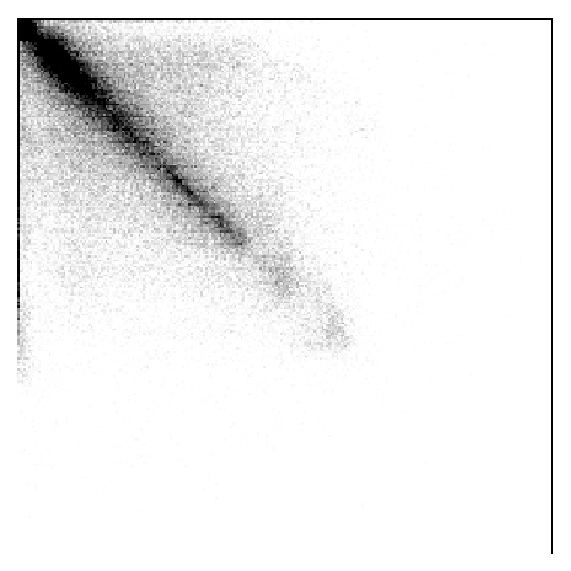
\includegraphics[width=0.2\textwidth]{3_review/figures/processing/registration/histogram/jointhistomisal.eps}}
\hspace*{\fill}
	\caption[Difference observed in joint histogram between aligned and misaligned images.]{Difference observed in joint histogram between aligned and misaligned images. The joint measure will be more concentrated of the histogram in the case that the images are aligned and more randomly distributed in the case that both images are more misaligned.}
        \label{fig:jointhisto}
\end{figure}

In this regard, \ac{mi} has been introduced as a similarity measure in registration framework in the late 1990's by \citeauthor{Pluim2003}.
The \ac{mi} measure finds its foundation in the assumption that a homogeneous region in the first modality image should also appear as a homogeneous region in the second modality, even if their \acp{si} are not identical.
Thus, those regions share information and the registration task is achieved by maximizing this common information.
Hence, \Ac{mi} of two images $A$ and $B$ is defined as:

\begin{equation}
	MI(A;B) = S(A) + S(B) - S(A,B) \ ,
	\label{eq:midef}
\end{equation}

\noindent where $S(A)$, $S(B)$, and $S(A,B)$ are the marginal entropies of $A$ and $B$ and the joint entropy, respectively.
Therefore, maximizing the \ac{mi} is the equivalent of minimizing the joint entropy. 
The joint entropy measure is related to the degree of uncertainty or dispersion of the data in the joint histogram of the images $A$ and $B$.
As shown in \acs{fig}\,\ref{fig:jointhisto}, the data in the joint histogram are concentrated in the case of aligned images (see \acs{fig}\,\ref{subfig:histoalgn}) while it is more randomly distributed in the case of misaligned images (see \acs{fig}\,\ref{subfig:histomisalgn}).
The entropy is computed based on an estimation of the \ac{pdf} of the images and thus histogram or Parzen window methods are a common way to estimate these \acp{pdf}.

A generalized form of \ac{mi}, \ac{cmi}, has been proposed by \citeauthor{Chappelow2011}.
\ac{cmi} encompasses interdependent information such as texture and gradient information into the metric.
Hence, for both of images $A$ and $B$, the image ensembles $\epsilon^{A}_n$ and $\epsilon^{B}_m$ are generated and composed of $n$ and $m$ images based on the texture and gradient.
Then, the \ac{cmi} is formulated such as:

\begin{equation}
	CMI(\epsilon^{A}_n;\epsilon^{B}_m) = S(\epsilon^{A}_n) + S(\epsilon^{B}_m) - S(\epsilon^{A}_n,\epsilon^{B}_m) \ .
	\label{eq:cmidef}
\end{equation}

From \acs{eq}\,\eqref{eq:cmidef}, note that \ac{cmi} is estimated from high-dimensional data and as a consequence the histogram-based methods to estimate the \acp{pdf} are not suitable anymore~\cite{Chappelow2011}. 
However, other alternative approaches are used such as the one employed in~\cite{Staring2009} to compute the $\alpha$-\ac{mi}~\cite{Hero2002}.
% which is based on the construction of entropic graphs which uses a \ac{knn} inside the high-dimensional feature space later used to estimate the \ac{mi}.

%\item[$-$] \textbf{\textit{Optimization methods:}} 
\paragraph{Optimization methods}
Registration is usually regarded as an optimization problem where the parameters of the geometric transformation model have to be inferred by minimizing/maximizing the similarity measure.
Iterative optimization methods are commonly used, where the most common methods used are the L-BFGS-B quasi-Newton method~\cite{Byrd1995} and the gradient descent~\cite{Viola1997}.
During our review, we noticed that authors do not usually linger over optimizer choice.

%\item[$-$] \textbf{\textit{Interpolation:}}
\paragraph{Interpolation} 
The registration procedure involves transforming an image and pixels mapped to non-integer points must be approximated using interpolation methods.
As for the optimization methods, we notice that little attention has been paid on the choice of those interpolations methods.
However, commonly used methods are bi-linear, nearest-neighbour, bi-cubic, spline, and inverse-distance weighting method~\cite{Mitra2012}.

%\item[$-$] \textbf{\textit{Registration methods used in \ac{cad} systems:}} 
\paragraph{Registration methods used in \ac{cad} systems}
\acs{tab}~\ref{tab:regtab} summarized the framework used to register \ac{mpmri} images in \ac{cad} for \ac{cap}.

\begin{table}
  \centering
  \caption[Classification of the different registration methods used in the \acs*{cad} systems reviewed.]{Classification of the different registration methods used in the \acs*{cad} systems reviewed. Acronyms: mean squared error (MSE), mutual information (MI), combined mutual information (CMI), gradient descent (GD), limited-memory Broyden-Fletcher-Goldfarb-Shannon box constraints (L-BFGS-B).}
  \scriptsize
    \begin{threeparttable}
      \begin{tabular}{l l c c c c c c c c}\hline
        \toprule
        \textbf{Study} & \textbf{Modality} & \multirow{2}{*}{\textbf{Type}} & \multicolumn{2}{c}{\textbf{Geometric model}} & \multicolumn{3}{c}{\textbf{Similarity measure}} & \multicolumn{2}{c}{\textbf{Optimizer}} \\
        \cmidrule{4-10}
        \textbf{index} & \textbf{registered} & & Affine & Elastic & \acs{mse} & \acs{mi} & \acs{cmi} & GD & L-BFGS-B \\
        \midrule
        \cite{Ampeliotis2007,Ampeliotis2008} & \ac{t2w} - \ac{dce} & 2D & \cmark & $-$ & \cmark & $-$ & $-$ & $-$ & $-$ \\
        \cite{Giannini2013,giannini2015fully} & \ac{t2w} - \ac{dw} & 2D & \cmark & \cmark & $-$ & $-$ & $-$ & $-$ & $-$  \\
        \cite{Giannini2013,giannini2015fully} & \ac{t2w} - \ac{dce} & 2D & \cmark & \cmark & $-$ & \cmark & $-$ & \cmark & $-$ \\
        \cite{Viswanath2008a,Viswanath2009} & \ac{t2w} - \ac{dce} & 2D & \cmark & $-$ & $-$ & \cmark & $-$ & $-$ & $-$ \\
        \cite{Viswanath2011} & \ac{t2w} - \ac{dce} - \ac{dw} & 3D & \cmark & $-$ & $-$ & $-$ & \cmark & \cmark & $-$  \\
        \cite{Vos2008} & \ac{t2w} - \ac{dce} & 3D & \cmark & $-$ & $-$ & \cmark & $-$ & $-$ & $-$ \\
        \cite{Vos2010} & \ac{t2w} - \ac{dce} & 3D & \cmark & \cmark & $-$ & \cmark & $-$ & $-$ & \cmark \\
        \bottomrule
      \end{tabular}
      \begin{tablenotes}
        \footnotesize
      \item Notes:
      \item {$-$}: not used or not mentioned.
      \item {\cmark}: used or implemented.
      \end{tablenotes}
    \end{threeparttable}
\label{tab:regtab}  
\end{table}

\citeauthor{Ampeliotis2008} in~\cite{Ampeliotis2007,Ampeliotis2008} did not use the framework as presented in \acs{fig}\,\ref{fig:frareg} to register 2D \ac{t2w}-\ac{mri} and \ac{dce}-\ac{mri} images.
By using image symmetries and the \ac{mse} metric, they found the parameters of an affine transformation but without using a common objective function.
The scale factor, the rotation, and the translation are independently and sequentially estimated.

\cite{Giannini2013} used also a in-house registration method for 2D \ac{t2w}-\ac{mri} and \ac{dw}-\ac{mri} images using an affine model~\cite{Giannini2013,giannini2015fully}.
The bladder is first segmented in both modalities in order to obtain its contours and to focus on the registration and minimize the distance between the contours.

\citeauthor{Giannini2013} and also \citeauthor{Vos2010} used a framework based on finding an affine transformation to register the \ac{t2w}-\ac{mri} and \ac{dce}-\ac{mri} images using \ac{mi}~\cite{Rueckert1999,Giannini2013,Vos2010}.
Then, an elastic registration using B-spline takes place using the affine parameters to initialize the geometric model with the same similarity measure.
However, the two approaches differ regarding the choice of the optimizer since a gradient descent is used in~\cite{Giannini2013} and a quasi-Newton method in~\cite{Vos2010}.
Moreover, \citeauthor{Giannini2013} applied a 2D registration whereas \citeauthor{Vos2010} registered 3D volumes.

\citeauthor{Viswanath2008a} as well as \citeauthor{Vos2008} registered \ac{t2w}-\ac{mri} and \ac{dce}-\ac{mri} images using an affine registration and a \ac{mi} metric~\cite{Viswanath2008a,Viswanath2009,Vos2008}.
However, the choice of the optimizer has not been specified. 
Furthermore, \citeauthor{Viswanath2008a} focused on 2D registration~\cite{Viswanath2008a,Viswanath2009} while \citeauthor{Vos2008} performed 3D registration~\cite{Vos2008}.

Finally, \citeauthor{Viswanath2011} performed a 3D registration with the three modalities, \ac{t2w}-\ac{mri}, \ac{dce}-\ac{mri}, and \ac{dw}-\ac{mri}, using an affine transformation model combined with the \ac{cmi} similarity measure~\cite{Viswanath2011}.
Moreover, in this latter work, the authors employed a gradient descent approach~\cite{Chappelow2011} to solve this problem but suggested that the Nelder-Mead simplex and the quasi-Newton methods are other possible solutions.

%\end{enumerate}

\section{Image classification framework}\label{sec:chp3:img-clas}


\subsection{\acs*{cade}: \acsp*{roi} detection/selection} \label{subsec:chp3:img-clas:roiSel}

\begin{table}
  \caption{Overview of the \acs*{cade} strategies employed in \acs*{cad} systems.}
  \scriptsize
  \centering
  \begin{tabularx}{\textwidth}{l >{\raggedleft\arraybackslash}X}
    \toprule
    \textbf{\ac{cade}: \acp{roi} selection strategy} & \textbf{References} \\
    \midrule
    All voxels-based approach & \cite{Artan2009,Artan2010,Giannini2013,Kelm2007,Liu2009,Lopes2011,Matulewicz2013,Mazzetti2011,Ozer2009,Ozer2010,Parfait2012,Sung2011,Tiwari2007,Tiwari2008,Tiwari2009,Tiwari2009a,Tiwari2010,Tiwari2012,Tiwari2013,Viswanath2008,Viswanath2008a,Viswanath2009,Viswanath2011,Viswanath2012,trigui2016classification,trigui2017automatic,lehaire2014computer,khalvati2015automated,rampun2015classifying,rampun2015computer,rampun2016computer,rampun2016computerb,rampun2016quantitative} \\
    Lesions candidate detection & \cite{Litjens2011,Litjens2012,Litjens2014,Vos2012,cameron2014multiparametric,cameron2016maps} \\
    \bottomrule
  \end{tabularx}
\label{tab:cade}
\end{table}

As discussed in the introduction and shown in \acs{fig}\,\ref{fig:wkfcad}, the image classification framework is often composed of a \ac{cade} and a \ac{cadx}.
In this section, we focus on studies which embed a \ac{cade} in their framework.
Two approaches are considered to define a \ac{cade}: (i) voxel-based delineation and (ii) lesion segmentation.
These methods are summarized in \acs{tab}~\ref{tab:cade}.
The first strategy is in fact linked to the nature of the classification framework and concerns the majority of the studies reviewed~\cite{Artan2009,Artan2010,Giannini2013,Kelm2007,Liu2009,Lopes2011,Matulewicz2013,Mazzetti2011,Ozer2009,Ozer2010,Parfait2012,Sung2011,Tiwari2007,Tiwari2008,Tiwari2009,Tiwari2009a,Tiwari2010,Tiwari2012,Tiwari2013,Viswanath2008,Viswanath2008a,Viswanath2009,Viswanath2011,Viswanath2012,trigui2016classification,trigui2017automatic,lehaire2014computer,khalvati2015automated,rampun2015classifying,rampun2015computer,rampun2016computer,rampun2016computerb,rampun2016quantitative}.
Each voxel is a possible candidate and will be classified as cancer or healthy.
The second group of methods is composed of method implementing a lesion segmentation algorithm to delineate potential candidates to further obtain a diagnosis through the \ac{cadx}.
This approach is borrowed from other application areas such as breast cancer.
These methods are in fact very similar to the classification framework used in \ac{cadx} later.

\citeauthor{Vos2012} highlighted lesion candidates by detecting blobs in the \ac{adc} map~\cite{Vos2012}.
These candidates are filtered using some \textit{a priori} criteria such as \ac{si} or diameter.
As mentioned in \acs{sec}\,\ref{subsec:chp2:imaging:mrsi} and \acs{tab}~\ref{tab:modmri}, low \ac{si} in \ac{adc} map can be linked to potential \ac{cap}.
Hence, blob detectors are suitable to highlight these regions. 
Blobs are detected in a multi-resolution scheme, by computing the three main eigenvalues $\{ \lambda_{\sigma,1},\lambda_{\sigma,2},\lambda_{\sigma,3} \}$ of the Hessian matrix, for each voxel location of the \ac{adc} map at a specific scale $\sigma$~\cite{Li2003}.
The probability $p$ of a voxel $\mathbf{x}$ being a part of a blob at the scale $\sigma$ is given by:

\begin{equation}
P(\mathbf{x},\sigma) = \begin{cases}
	\frac{\| \lambda_{\sigma,3}(\mathbf{x}) \|^{2}}{\| \lambda_{\sigma,1} (\mathbf{x}) \|} \ , & \text{if } \lambda_{\sigma,k}(\mathbf{x}) > 0 \text{ with } k = \{1,2,3\} \  , \\
	0 \ , & \text{otherwise} \ .
\end{cases}
\label{eq:blobdet}
\end{equation}

\noindent The fusion of the different scales is computed as:

\begin{equation}
	L(\mathbf{x}) = \max P(\mathbf{x},\sigma) , \forall \sigma \ .
	\label{eq:fusionBlob}
\end{equation}

The candidate blobs detected are then filtered depending on their appearances --- i.e., maximum of the likelihood of the region, diameter of the lesion --- and their \ac{si} in \ac{adc} and \ac{t2w}-\ac{mri} images.
The detected regions are then used as inputs for the \ac{cadx}.
\citeauthor{cameron2016maps} used a similar approach by automatically selecting low \ac{si} connected regions in the \ac{adc} map with a size larger than \SI{1}{\milli\metre\squared}~\cite{cameron2014multiparametric,cameron2016maps}.

\citeauthor{Litjens2011} used a pattern recognition approach in order to delineate the \acp{roi}~\cite{Litjens2011}.
A blobness map is computed in the same manner as in~\cite{Vos2010} using the multi-resolution Hessian blob detector on the \ac{adc} map, \ac{t2w}, and pharmacokinetic parameters maps (see \acs{sec}\,\ref{subsec:chp3:img-clas:CADX-fea-dec} for details about those parameters).
Additionally, the position of the voxel $\mathbf{x}=\{x,y,z\}$ is used as a feature as well as the Euclidean distance of the voxel to the prostate center.
Hence, each feature vector is composed of 8 features and a \ac{svm} classifier is trained using a \ac{rbf} kernel (see \acs{sec}\,\ref{subsec:chp3:img-clas:CADX-clas} for more details).

Subsequently, \citeauthor{Litjens2012} modified this approach by including only features related to the blob detection on the different maps as well as the original \acp{si} of the parametric images~\cite{Litjens2012}.
Two new maps are introduced based on texture and a \ac{knn} classifier is used instead of a \ac{svm} classifier
The candidate regions are then extracted by performing a local maxima detection followed by post-processing region-growing and morphological operations. 

\subsection{\acs*{cadx}: Feature detection} \label{subsec:chp3:img-clas:CADX-fea-dec}

Discriminative features which help to recognize \ac{cap} from healthy tissue need to be first detected.
This processing is known in computer vision as feature extraction. 
However, feature extraction also refer to the name given in pattern recognition to some types of dimension reduction methods which are later presented.
In order to avoid confusion between these two aspects, in this survey, the procedure ``detecting'' or ``extracting'' features from images and signals is defined as feature detection.
This section summarizes the different features used in \ac{cad} for \ac{cap} and are summarized in \acs{tab}~\ref{tab:feat}.  

\input{3_review/Table-CADX-feature-detection}

\subsubsection{Image-based features}\label{subsubsec:chp3:img-clas:CADX-fea-dec:Img-fea}

This section focuses on image-based features which can be categorized into two categories: (i) voxel-wise detection and (ii) region-wise detection.

\paragraph{Voxel-wise detection}
This strategy refers to the fact that a feature is extracted at each voxel location.
As discussed in \acs{sec}\,\ref{sec:chp2:imaging}, \ac{cap} has an influence on the \ac{si} in \ac{mpmri} images.
Therefore, intensity-based feature is the most commonly used feature~\cite{Ampeliotis2007,Ampeliotis2008,Vos2008,rampun2016computerb,rampun2015classifying,Giannini2013,Artan2009,Artan2010,Chan2003,Langer2009,Litjens2011,Litjens2012,Litjens2014,Liu2009,Ozer2009,Ozer2010,trigui2016classification,trigui2017automatic,cameron2014multiparametric,cameron2016maps,khalvati2015automated,chung2015prostate,giannini2015fully,Niaf2011,Niaf2012,lehaire2014computer}.
This feature consists in the extraction of the intensity of the \ac{mri} modality of interest.

Edge-based features have also been used to detect \ac{si} changes but bring additional information regarding the the \ac{si} transition.
Each feature is computed by convolving the original image with an edge operator.
Three operators are commonly used: (i) Prewitt operator~\cite{Prewitt1970}, (ii) Sobel operator~\cite{Sobel1970}, and (iii) Kirsch operator~\cite{Kirsch1971}.
These operators differ due to the kernel used which attenuate more or less the noise.
Multiple studies used the resulting magnitude and orientation of the edges computed in their classification frameworks~\cite{Niaf2011,Niaf2012,Tiwari2009a,Tiwari2010,Tiwari2013,Viswanath2008,Viswanath2011,rampun2016quantitative,rampun2015computer,rampun2016computer,lehaire2014computer,khalvati2015automated,chung2015prostate}.

\begin{figure}
	\hspace*{\fill}
		\subfigure[$\theta=0^{\circ}$.]{\label{subfig:gab1} 
\includegraphics[width=0.2\linewidth]{3_review/figures/feature-detection/gabor/gabor_1.eps}} \hfill
		\subfigure[$\theta=60^{\circ}$.]{\label{subfig:gab2} 
\includegraphics[width=0.2\linewidth]{3_review/figures/feature-detection/gabor/gabor_2.eps}} \hfill
		\subfigure[$\theta=120^{\circ}$.]{\label{subfig:gab3} \includegraphics[width=0.2\linewidth]{3_review/figures/feature-detection/gabor/gabor_3.eps}} \hfill
		\subfigure[$\theta=180^{\circ}$.]{\label{subfig:gab4} \includegraphics[width=0.2\linewidth]{3_review/figures/feature-detection/gabor/gabor_4.eps}}
	\hspace*{\fill}
	\caption[Illustration of 4 different Gabor filters.]{Illustration of 4 different Gabor filters varying their orientations $\theta$.}
	\label{fig:gabor}
\end{figure}

Gabor filter~\cite{Gabor1946,Daugman1985} offer an alternative to the usual edge detector, with the possibility to tune the direction and the frequency of the filter to encode a specific pattern. 
A Gabor filter is defined by the modulation of a Gaussian function with a sine wave which can be further rotated and is formalized as in \acs{eq}\,\ref{eq:gabor}.
\begin{equation}
	g(x,y;\theta,\psi,\sigma,\gamma) = \exp \left( - \frac{x'^{2}+ \gamma^{2}y'^{2}}{2 \sigma^{2}} \right) \cos \left( 2 \pi \frac{x'}{\lambda} + \phi \right) \ ,
        \label{eq:gabor}
\end{equation}

\noindent with 

\begin{eqnarray}
	x' & = & s\left( x \cos \theta + y \sin \theta \right) \ , \nonumber \\
	y' & = & s \left( - x \sin \theta + y \cos \theta \right) \ , \nonumber
\end{eqnarray}

\noindent where $\lambda$ is the wavelength of the sinusoidal factor, $\theta$ represents the orientation of the Gabor filter, $\psi$ is the phase offset, $\sigma$ is the standard deviation of the Gaussian envelope, $\gamma$ is the spatial aspect ratio, and $s$ is the scale factor.
In an effort to characterize pattern and texture, a bank of Gabor filters is usually created with different angles, scale, and frequency --- refer to \acs{fig}\,\ref{fig:gabor} --- and then convolved with the image.
\citeauthor{Viswanath2012}, \citeauthor{Tiwari2012} and more recently \citeauthor{khalvati2015automated} and \citeauthor{chung2015prostate} have designed a bank of Gabor filters to characterized texture and edge information in \ac{t2w}-\ac{mri} and \ac{dw}-\ac{mri} modalities.

%%%% GO here 
\citeauthor{rampun2016computer} employed rotationally invariant Gabor filter banks ( \ac{lm}~\cite{varma2005statistical}) which takes edges and sopts/bars into account. 
The \ac{lm} consists of 48 filters including first and second derivatives of Gaussian at 6 orientations and 3 scales (36 filters), in addition to 8 Laplacian of Gaussian and 4 Gaussians filters.
The scale of proposed filters vary between $\sigma = 1$ to $\sigma = 10$ \si{\px}


Texture-based features provide other characteristics discerning \ac{cap} from healthy tissue.
The most common texture analysis for image classification is based on the \ac{glcm} with their related statistics which have been proposed by \citeauthor{Haralick1973} in~\cite{Haralick1973}.
In a neighborhood around a central voxel, a \ac{glcm} is build considering each voxel pair defined by a specific distance and angle.
Then, using the \ac{glcm}, a set of statistical features is computed as defined in \acs{tab}~\ref{tab:glcm} and assigned to the location of the central voxel.
Therefore, $N$ --- up to 14 --- statistical maps are derived from the \ac{glcm} analysis, one per statistics presented in \acs{tab}~\ref{tab:glcm}.
\ac{glcm} is commonly used in \ac{cad} systems, on the different \ac{mri} modalities, namely \ac{t2w}-\ac{mri}, \ac{dce}-\ac{mri}, or \ac{dw}-\ac{mri}~\cite{Antic2013,Niaf2011,Niaf2012,Tiwari2009a,Tiwari2010,Tiwari2013,Viswanath2008,Viswanath2009,Viswanath2011,Viswanath2012,trigui2016classification,rampun2015computer,rampun2016computer,rampun2016quantitative,cameron2014multiparametric,cameron2016maps,khalvati2015automated,chung2015prostate,lehaire2014computer}.
However, the statistics extracted from the \ac{glcm} across studies vary.

\begin{table}
  \caption[The 14 statistical features used in conjunction with \acs*{glcm} analysis.]{The 14 statistical features for texture analysis commonly computed from the \acs*{glcm} $p$ as presented by~\cite{Haralick1973}.}
  \scriptsize
  \renewcommand{\arraystretch}{1.5}
  \centering
  \begin{tabular}{ll}
    \toprule
    \textbf{Statistical features} & \textbf{Formula} \\
    \midrule
    Angular second moment & $\sum_i \sum_j p(i,j)^2 $  \\
    Contrast & $\sum_{n=0}^{N_g - 1} n^2 \left[ \sum_{i=1}^{N_g - 1} \sum_{j=1}^{N_g - 1} p(i,j) \right] \ , | i-j |=n  $ \\
    Correlation & $\frac{\sum_i \sum_j (ij) p(i,j) - \mu_x \mu_y}{\sigma_x \sigma_y}  $ \\
    Variance & $\sum_i \sum_j (i - \mu)^2 p(i,j)  $ \\
    Inverse difference moment & $\sum_i \sum_j \frac{1}{1+(i - \mu)^2} p(i,j)  $ \\
    Sum average & $\sum_{i=2}^{2N_g} i p_{x+y}(i)  $ \\
    Sum variance & $\sum_{i=2}^{2N_g} (i-f_s)^2 p_{x+y}(i)  $ \\
    Sum entropy & $ - \sum_{i=2}^{2N_g} p_{x+y}(i) \log p_{x+y}(i)  $ \\
    Entropy & $ - \sum_i \sum_j p(i,j) \log p(i,j) $ \\
    Difference variance & $\sum_{i=0}^{N_g-1} i^2 p_{x-y}(i)  $ \\
    Difference entropy & $ - \sum_{i=0}^{N_g-1} p_{x-y}(i) \log p_{x-y}(i)  $ \\
    Info. measure of corr. 1 & $\frac{S(X;Y)-S_1(X;Y)}{\max(S(X),S(Y))}  $ \\
    Info. measure of corr. 2 & $\sqrt{\left( 1 - \exp \left[ -2( H_2(X;Y) - H(X;Y) ) \right] \right)}  $ \\
    Max. corr. coeff. & $ \sqrt{\lambda_2} \ , \text{of } Q(i,j) = \sum_k \frac{p(i,k)p(j,k)}{p_x(i)p_y(k)}  $ \\
    \bottomrule
  \end{tabular}
  \label{tab:glcm}
\end{table}

Fractal analysis and more precisely a local estimation of the fractal dimension \cite{Benassi1998} describing the texture roughness at a specific location was used in \cite{Lopes2011}.
A wavelet-based method in a multi-resolution framework was used to estimate the fractal dimension.
Cancerous tissue were characterized to have a higher fractal dimension than healthy tissue.

Chan \textit{et al.}~\cite{Chan2003} described the texture using the frequency signature via the \acf{dct} \cite{Ahmed1974}) defining a neighbourhood of $7 \times 7$ pixels for each of the modalities that they used.
The \ac{dct} allows to decompose a portion of image into a coefficients space where few of these coefficients encoded the visually significant information.
The \ac{dct} coefficients are computed such as:

\begin{equation}
	C_{k_1,k_2} = \sum_{m=0}^{M-1} \sum_{n=0}^{N-1} p_{m,n} \cos \left[ \frac{\pi}{M} \left( m + \frac{1}{2} \right) k_1 \right] \cos \left[ \frac{\pi}{N} \left( n + \frac{1}{2} \right) k_2 \right] \ ,
\end{equation}

\noindent where $C_{k_1,k_2}$ is the \ac{dct} coefficient at the position $k_1,k_2$, $M$ and $N$ are the dimension of the neighbourhood and $p_m,n$ is the pixel \ac{si} at the position $p_{m,n}$.

Viswanath \textit{et al.}~\cite{Viswanath2012} projected \ac{t2w} images into the wavelet space, using Haar wavelet, and used the coefficients obtained from the decomposition as features.
%The wavelet family used for the decomposition was the Haar wavelet.

Finally Litjens \textit{et al.} in \cite{Litjens2011} computed the texture map based on \ac{t2w} images using a Gaussian filer bank.
%% Euclidean distance from each voxel to the prostate center as well as the individual distance in the three directions $x$, $y$ and $z$. \cite{Chan2003} embedded the same information but this time using cylindrical coordinate $r$, $\theta$ and $z$ corresponding to the radius, azimuth and elevation respectively.


\paragraph{Region-wise detection}

Unlike the previous section, another strategy is to study an entire region and extract characteristic features corresponding to this region.
The most common approach reviewed can be classified as statical methods.
First a feature map is computed for the whole image instaed of using single voxels.
Then, \acp{roi} are defined and statistics are extracted from each of these regions.
The most widely used statistics is based on percentiles and is widely used \cite{Antic2013,Litjens2011,Litjens2012,Litjense2014,Peng2013,Tiwari2009a,Tiwari2010,Tiwari2013,Viswanath2008,Viswanath2008a,Viswanath2011,Viswanath2012,Vos2008,Vos2008a,Vos2010,Vos2012}.
The percentile used is usually manually determined observing the distribution and corresponds to the best discriminant value differentiating malignant and healthy tissue.
In addition, statistic-moments such as mean, standard deviation, kurtosis and skewness are also used \cite{Ampeliotis2007,Ampeliotis2008,Antic2013,Niaf2011,Niaf2012,Peng2013}.
Litjense \textit{et al.} in \cite{Litjense2014} also introduced a feature based on symmetry.
They compute the mean of a candidate lesion as well as its mirrored counter-part and compute the quotient as feature.

Another subset of features are anatomic which were also used in \cite{Litjens2012,Litjense2014,Matulewicz2013}. 
Litjense \textit{et al.} in \cite{Litjense2012, Litjense2014} computed the volume, compactness and sphericity related to the region to integrate it in their feature vector.
Matulewicz \textit{et al.}~\cite{Matulewicz2013} introduced four features corresponding to the percentage of tissue belonging to the regions\ac{pz}, \ac{cg}, periurethral region or outside prostate region for the considered \ac{roi}.

In contrast to anatomical are histogram-based features.
For instance, Liu \textit{et al.}~\cite{Liu2013} introduced four different types of histogram-based features.
The first type corresponds to the histogram of the \ac{si} of the image.
The second type is the \acf{hog} \cite{Dalal2005}.
\Ac{hog} descriptor describes the local shape of the object of interest by using distribution of gradient directions.
This descriptor is extracted mainly in three steps.
First the gradient image and its corresponding magnitude and direction are computed.
Then, the \ac{roi} is divided into cells and an oriented-based histogram is generated for each cell.
At each pixel location, the orientation of the gradient will vote for a bin of the histogram and this vote is weighted by the magnitude of the same gradient.
Finally, The cells are grouped into block and each block is normalized.
The third histogram-based type used in \cite{Liu2013} was shape context \cite{Belongie2002}.
The shape context is also a way to describe the shape of an object of interest.
First, a set of points defining edges have to be detected and for each point of each edge, a log-polar-based histogram is computed using the relative points distribution.
The last set of histogram-based feature extracted is based on the framework described in \cite{Zhao2012} which is using the Fourier transform of the histogram created via \acf{lbp} \cite{Ojala1996}.
\Ac{lbp} is generated by comparing the value of the central pixel with its 8-connected neighbours.
Then, in the \ac{roi}, the histogram of the \ac{lbp} distribution is computed.
The \acf{dft} of the \ac{lbp} histogram is used to make the feature invariant to rotation.

The last group of region-based feature is based on fractal analysis.
The features proposed are based on estimating the fractal dimension which is a statistical index representing the complexity of what is analysed.
Lv \textit{et al,}~\cite{Lv2009} proposed two features based on fractal dimension: (i) texture fractal dimension and (ii) histogram fractal dimension.
The first feature is based on estimating the fractal dimension on the \ac{si} of each image.
Hence, this feature is a statistical characteristic of the image roughness.
The second fractal dimension is estimated in the \ac{pdf} of each image and characterises the complexity of the \ac{pdf}.
Lopes \textit{et al.}~\cite{Lopes2011} proposed a 3D version to estimate the fractal dimension of a volume using wavelet decomposition.


\subsubsection{\Ac{dce}-based features}\label{subsubsec:chp3:img-clas:CADX-fea-dec:DCE-fea}

\ac{dce}-\ac{mri} is more commonly based on a \ac{si} analysis over time as presented in Sect.~\ref{subsec:chp2:imaging:dce}.
In this section the features extracted for \ac{dce}-\ac{mri} analysis are presented.

\begin{table}
  \caption{Parameters used as features for a \acs*{dce} semi-quantitative analysis in \acs*{cad} systems.}
  \scriptsize
  \centering
  \begin{tabularx}{\textwidth}{l X}
    \toprule
    \textbf{Semi-quantitative features} & \textbf{Explanations} \\
    \midrule
    \textbf{Amplitude features:} & \\ \\ [-1.5ex]
    \quad $\bullet\ S_0$ & Amplitude at the onset of the enhancement \\
    \quad $\bullet\ S_{\max}$ & Amplitude corresponding to $95\%$ of the maximum amplitude \\
    \quad $\bullet\ S_{p}$ & Amplitude corresponding to the maximum amplitude \\
    \quad $\bullet\ S_f$ & Amplitude at the final time point \\ \\ [-1.5ex]
    \textbf{Time features:} & \\ \\ [-1.5ex]
    \quad $\bullet\ t_0$ & Time at the onset of the enhancement \\
    \quad $\bullet\ t_{\max}$ & Time corresponding to $95\%$ of the maximum amplitude \\
    \quad $\bullet\ t_{p}$ & Time corresponding to the maximum amplitude \\
    \quad $\bullet\ t_{f}$ & Final time \\
    \quad $\bullet\ t_{tp}$ & Time to peak which is the time from $t_0$ to $t_p$ \\ \\ [-1.5ex]
    \textbf{Derivatives and integral features:} & \\ \\ [-1.5ex]
    \quad $\bullet\ WI$ & Wash-in rate corresponding to the signal slope from $t_0$ to $t_m$ or $t_p$ \\
    \quad $\bullet\ WO$ & Wash-out rate corresponding to the signal slope from $t_m$ or $t_p$ to $t_p$ \\
    \quad $\bullet\ IAUC$ & Initial area under the curve which is the area between $t_0$ to $t_{f}$ \\
    \bottomrule
  \end{tabularx}
\label{tab:semiqua}
\end{table}


\paragraph{Whole-spectra approach}
Some studies are using the whole \ac{dce} time series as feature vector \cite{Ampeliotis2007,Ampeliotis2008,Tiwari2012,Viswanath2008a,Viswanath2008}.
In some cases, the high-dimensional feature space is reduced using dimension reduction methods as it will be presented in the next section (see Sect.~\ref{subsec:chp3:img-clas:CADX-fea-ext}).

\begin{figure}
	\centering
	\includegraphics[width=.8\linewidth]{3_review/figures/feature-detection/dce/dce_cancer_parameters.eps}
	\caption[Semi-quantitative features used for \acs*{dce}-\acs*{mri}.]{Graphical representation of the different semi-quantitative features used for \acs*{dce}-\acs*{mri} analysis.}
	\label{fig:dceparam}
\end{figure}

\paragraph{Semi-quantitative approach}
Semi-quantitative approaches are based on mathematically modelling the \ac{dce} time series.
The parameters modelling the signal are commonly used, mainly due to the simplicity of their computation.
Parameters included in semi-quantitative analysis are summarized in Tab.~\ref{tab:semiqua} and also graphically depicted in Fig.~\ref{fig:dceparam}.
A set of time features corresponding to specific amplitude level (start, maximum and end) are extracted.
Then, derivative and integral features are also considered as discriminative and are commonly computed.


\paragraph{Quantitative approach}
As presented in Sect.~\ref{sec:chp2:imaging}, quantitative approaches correspond to mathematical-pharmacokinetic models based on physiological exchanges.
Four different models have been used in \ac{cad} for \ac{cap} systems.
The most common model reviewed was the \textit{Brix model} \cite{Artan2009,Artan2010,Sung2011,Liu2009,Ozer2009,Ozer2010}.
This model is formalized such as:
\begin{equation}
	\frac{S(t)}{S(0)} = 1 + A k_{ep} \left( \frac{\exp( -k_{ep} t ) - \exp( -k_{el} t )}{k_{el} - k_{ep}} \right) \ ,
	\label{eq:brixmod}
\end{equation}

\noindent where $S(\cdot)$ is the \ac{dce} signal, $A$ is the parameter simulating the tissue properties, $k_{el}$ is the parameter related to the first-order elimination from the plasma compartment and $k_{ep}$ is the parameter of the transvascular permeability.
These parameters ($k_{ep}$, $k_{el}$,$A$) are computed from the \ac{mri} data and used as features.

Another model is Tofts model \cite{Tofts1997} which was used in \cite{Langer2009,Giannini2013,Niaf2011,Niaf2012,Mazzetti2011}.
In this model, the \ac{dce} signal relative to the concentration is presented as:
\begin{equation}
	C_t(t) = v_p C_p(t) + K_{trans} \int_{0}^{t} C_p(\tau) \exp( -k_{ep}(t-\tau) ) \ d\tau \ ,
	\label{eq:tofts} 
\end{equation}

\noindent where $C_t(\cdot)$ is the concentration of the medium, $C_p(\cdot)$ is the \ac{aif} which have to be estimated independently, $K_{trans}$ is the parameter related to the diffuse transport of media across the capillary endothelium, $k_{ep}$ is the parameter related to the exchanges back into the vascular space and $v_e$ is the extravascular-extracellular space fraction defined such that $v_e = 1 - v_p$.
In this model, paramteres $K_{trans}$, $k_{ep}$ and $v_e$ are computed and used as features.

%Mazzetti \textit{et al.}~\cite{Mazzetti2011} and Giannini \textit{et al.}~\cite{Giannini2013} used the Weibull function empirically formalized as:
Mazzetti \textit{et al.}~\cite{Mazzetti2011} and Giannini \textit{et al.}~\cite{Giannini2013} used the Weibull function in different emprical model based on West-like function and referred to as the phenomenological universalities model \cite{Castorina2006} defined by three parameters $\beta$, $a_{0}$, and $r$ ( see Eq.~\ref{eq:pun}).

%% \begin{equation}
%% 	S(t) = A t \exp( -t^{B} ) \ ,
%% 	\label{eq:weibull}
%% \end{equation}

%% \noindent where $A$ and $B$ are the two parameters which have to be inferred.
%They also used another empirical model which is based on the West-like function and named the phenomenological universalities model \cite{Castorina2006}) formalized as:
\begin{equation}
	S(t) = \exp \left[ r t + \frac{1}{\beta} a_0 - r \left( \exp( \beta t ) - 1 \right) \right] \ ,
	\label{eq:pun}
\end{equation}
%\noindent where the parameters $\beta$, $a_0$ and $r$ are inferred.
\noindent For all these models, the parameters are inferred using an optimization curve fitting approach.


\subsubsection{\Ac{mrsi}-based features}\label{subsubsec:chp3:img-clas:CADX-fea-dec:MRSI-fea}

\paragraph{Whole spectra approach}
As in the case of \ac{dce} analysis, one common approach is to incorporate the whole \ac{mrsi} spectra in the feature vector for classification \cite{Kelm2007,Parfait2012,Tiwari2007,Tiwari2009,Tiwari2013,Tiwari2009a,Tiwari2010,Viswanath2008a,Matulewicz2013}. 
Sometimes post-processing involving dimension reduction methods is performed to reduce the complexity during the classification as it will be presented in Sect.~\ref{subsec:chp3:img-clas:CADX-fea-ext}.

\paragraph{Quantification approach}
We can reiterate that in \ac{mrsi} only few biological markers (cf., choline, creatine and citrate metabolites mainly) are known to be useful to discriminate \ac{cap} and healthy tissue.
Then, concentrations of these metabolites can be considered as a feature used for classification.
In order to perform this quantification, four different approaches have been used.
The QUEST \cite{Ratiney2005}, AMARES \cite{Vanhamme1997} and VARPRO \cite{Coleman1993} models were used in \cite{Kelm2007}.
They are all time-domain quantification methods varying by the type of pre-knowledge embedded and the optimization approaches used to solve the quantification problem.
Unlike the time-domain quantification approaches, Parfait \textit{et al.}~\cite{Parfait2012} used the LcModel approach \cite{Provencher1993}) which solves the optimization problem in the frequency domain.

Although Parfait \textit{et al.}~\cite{Parfait2012} used each metabolite concentration individually, other authors such as Kelm \textit{et al.}~\cite{Kelm2007} proposed to compute relative concentrations as the ratio of the choline plus creatine to citrate (see Eq.~\eqref{eq:ratio1}) or the ratio of citrate to choline plus creatine plus citrate (see Eq.~\eqref{eq:ratio2}).

\begin{eqnarray}
	R_1 & = & \frac{ [ \text{Cho} ] + [ \text{Cr} ]}{[ \text{Cit} ]} \ . \label{eq:ratio1} \\
	R_2 & = & \frac{[ \text{Cit} ]}{[\text{Cho}]+[\text{Cr}]+[\text{Cit}]} \ , \label{eq:ratio2}
\end{eqnarray}
\noindent where $\text{Cit}$, $\text{Cho}$ and $\text{Cr}$ are the concentration of citrate, choline and creatine respectively.

\paragraph{Wavelet decomposition approach} 
Tiwari \textit{et al.}~\cite{Tiwari2012} performed a wavelet packet decomposition \cite{Coifman1992} of the spectra with the Haar wavelet basis function and used its coefficients as features.

\subsection{\acs*{cadx}: Feature selection and feature extraction} \label{subsec:chp3:img-clas:CADX-fea-ext}
As presented in the previous section, it is a common practise to extract a wide variety of features.
While dealing with \ac{mpmri}, the feature space created is a high-dimensional space which might mislead or corrupt the classifier during the training phase.
Therefore, it is of interest to reduce the number of dimensions before proceeding to the classification task.
The strategies used can be grouped as: (i) feature selection and (ii) feature extraction.
In this section only the methods used in \ac{cad} system are presented and summarized in \acs{tab}~\ref{tab:featext}.

\begin{table}
  \caption{Overview of the feature selection and extraction methods used in \acs*{cad} systems.}
  \scriptsize
  \centering
  \begin{tabular}{l r}
    \toprule
    \textbf{Dimension reduction methods} & \textbf{References} \\
    \midrule
    \textbf{Feature selection:} & \\ \\ [-1.5ex]
    \quad Statistical test & \cite{Niaf2011,Niaf2012,Vos2012} \\
    \quad \ac{mi}-based methods & \cite{Niaf2011,Niaf2012,Vos2008,lehaire2014computer,khalvati2015automated,chung2015prostate} \\
    \quad Correlation-based methods & \cite{rampun2016computer,rampun2015computer} \\ \\ [-1.5ex]
    \textbf{Feature extraction:} & \\ \\ [-1.5ex]
    \quad Linear mapping & \\
    \quad \quad \acs*{pca} & \cite{Tiwari2008,Tiwari2009} \\
    \quad Non-linear mapping & \\
    \quad \quad Laplacian eigenmaps & \cite{Tiwari2007,Tiwari2009a,Tiwari2009,Tiwari2010,Viswanath2008,Viswanath2011} \\
    \quad \quad \acs*{lle} and \acs*{lle}-based & \cite{Tiwari2008,Tiwari2009,Viswanath2008a,Viswanath2008} \\
    \quad Dictionary-based learning & \\
    \quad \quad Sparse coding & \cite{lehaire2014computer} \\
    \quad \quad \acs*{bow} & \cite{rampun2016computerb,rampun2015classifying} \\
    \bottomrule
  \end{tabular}
\label{tab:featext}
\end{table} 

\subsubsection{Feature selection}\label{subsubsec:chp3:img-clas:CADX:fea-ext:sel}
The feature selection strategy is based on selecting the most discriminative feature dimensions of the high-dimensional space.
Thus, the low-dimensional space is then composed of a subset of the original features detected.
In this section, methods employed in \ac{cad} for \ac{cap} detection are presented.
A more extensive review specific to feature selection is available in~\cite{Saeys2007}.

\citeauthor{Niaf2012} make use of the p-value by using the independent two-sample t-test with equal mean for each feature dimension~\cite{Niaf2011,Niaf2012}.
In this statistical test, there are 2 classes: \ac{cap} and healthy tissue.
Hence, for each particular feature, the distribution of each class is characterized by their means $\bar{X}_1$ and $\bar{X}_2$ and standard deviation $s_{X_1}$ and $s_{X_2}$.
Therefore, the null hypothesis test is based on the fact that these both distribution means are equal.
The t-statistic used to verify the null hypothesis is formalized such that:

\begin{eqnarray}
t & = & \frac{\bar {X}_1 - \bar{X}_2}{s_{X_1X_2} \cdot \sqrt{\frac{1}{n_1}+\frac{1}{n_2}}} \ , \label{eq:tstat} \\
s_{X_1X_2} & = & \sqrt{\frac{(n_1-1)s_{X_1}^2+(n_2-1)s_{X_2}^2}{n_1+n_2-2}} \ , \nonumber
\end{eqnarray}

\noindent where $n_1$ and $n_2$ are the number of samples in each class.
From \acs{eq}\,\eqref{eq:tstat}, more the means of the class distribution diverge, the larger the $t$-statistic $t$ will be, implying that this particular feature is more relevant and able to make the distinction between the two classes. 

The $p$-value statistic is deduced from the $t$-test and corresponds to the probability of obtaining such an extreme test assuming that the null hypothesis is true~\cite{Goodman1999}.
%Hence, smaller the $p$-value, the more likely we are to reject the null hypothesis and more relevant the feature is likely to be.
Hence, smaller the $p$-value, the more likely the null hypothesis to be rejected the null hypothesis and more relevant the feature is likely to be.
Finally, the features are ranked and the most significant features are selected.
However, this technique suffers from a main drawback since it assumes that each feature is independent, which is unlikely to happen and introduces a high degree of redundancy in the features selected.

\citeauthor{Vos2012} in~\cite{Vos2012} employed a similar feature ranking approach but make use of the Fisher discriminant ratio to compute the relevance of each feature dimension.
Taking the aforementioned formulation, the Fisher discriminant ratio is formalized as the ratio of the interclass variance to the intraclass variance as:

\begin{equation}
F_r = \frac{\bar{X}_1 - \bar{X}_2}{s^{2}_{X_1}+s^{2}_{X_2}} \ .
\label{eq:fisherratio}
\end{equation}

Therefore, a relevant feature dimension is selected when the interclass variance is maximum and the intraclass variance in minimum.
Once the features are ordered, the authors select the feature dimensions with the largest Fisher discriminant ratio.

\Ac{mi} is a possible metric to use for selecting a subset of feature dimensions.
This method has previously been presented in \acs{sec}\,\ref{subsec:chp3:img-reg:reg} and expressed in \acs{eq}\,\eqref{eq:midef}.
%%%% As previously presented in Sect.~\ref{subsec:chp3:img-reg:reg} (see Eq.~\eqref{eq:midef}), the computation of the entropies involves the estimation of some \acp{pdf} and the data being usually continous variables, it is then necessary to estimate the \acp{pdf} using a method such as Parzen windows.
%%%% Definition of the \ac{mi} was presented in Sect.~\ref{subsec:chp3img-reg:reg} and formalized in Eq. \eqref{eq:midef} and as previously mentioned, the computation of the entropies involves the estimation of some \acp{pdf} and the data being usually continuous variables, it is then necessary to estimate the \acp{pdf} using a method such as Parzen windows.
\citeauthor{Peng2005} introduced two main criteria to select the feature dimensions based on \ac{mi}: (i) maximal relevance and (ii) minimum redundancy.
Maximal relevance criterion is based on the paradigm that the classes and the feature dimension which has to be selected have to share a maximal \ac{mi} and is formalized as:
\begin{equation}
  \argmax Rel(\mathbf{x},c) = \frac{1}{|\mathbf{x}|} \sum_{x_i \in \mathbf{x}} MI(x_i,c)  \ , 
  \label{eq:mRel}
\end{equation}
\noindent where $\mathbf{x} = \{x_i; i=1,\cdots,d\}$ is a feature vector of $d$ dimensions and $c$ is the class considered.
As in the previous method, using maximal relevance criterion alone imply an independence between each feature dimension.
The minimal redundancy criterion enforce the selection of a new feature dimension which shares as little as possible \ac{mi} with the previously selected feature dimensions such that:
\begin{equation}
  \argmin Red(\mathbf{x}) = \frac{1}{|\mathbf{x}|^2} \sum_{x_i,x_j \in \mathbf{x}} MI(x_i,x_j)  \ . 
  \label{eq:mRed}
\end{equation}
Combination of these two criteria is known as the \ac{mrmr} algorithm~\cite{Peng2005}.
Two combinations are usually used: (i) the difference or (ii) the quotient.
This method has been used at several occasions for the selecting a subset of features prior to classification~\cite{Niaf2011,Niaf2012,lehaire2014computer,Viswanath2012,khalvati2015automated,chung2015prostate}.

{\color{red} add a couple of sentence about correlation-based feature selection used by Rampun}.

\subsubsection{Feature extraction}\label{subsubsec:chp3:img-clas:CADX:fea-ext:ext}
The feature extraction strategy is related to dimension reduction methods but not selecting discriminative features.
Instead, these methods aim at mapping the data from the high-dimensional space into a low-dimensional space to maximize the separability between the classes.
As in the previous sections, only methods employed in \ac{cad} system are reviewed in this section.
We refer the reader to~\cite{Fodor2002} for a full review of feature extraction techniques.

\ac{pca} is the most commonly used linear mapping method in \ac{cad} systems.
\ac{pca} is based on finding the orthogonal linear transform mapping the original data into a low-dimensional space.
The space is defined such that the linear combinations of the original data with the $k^{th}$ greatest variances lie on the $k^{th}$ principal components~\cite{Jolliffe2002}.
The principal components are computed by using the eigenvectors-eigenvalues decomposition of the covariance matrix.
Let $\mathbf{x}$ denote the data matrix.
Then, the covariance matrix and eigenvectors-eigenvalues decomposition are defined as in \acs{eq}\,\eqref{eq:covmat}, and \acs{eq}\,\eqref{eq:eigpca}, respectively. 
The eigenvectors-eigenvalues decomposition can be formalized as:
\begin{equation}
  \Sigma = \mathbf{x}^{\text{T}} \mathbf{x} \ .
  \label{eq:covmat}
\end{equation}

\begin{equation}
  \mathbf{v}^{-1} \Sigma \mathbf{v} = \Lambda \ ,
  \label{eq:eigpca}
\end{equation}
\noindent where $\mathbf{v}$ are the eigenvectors matrix and $\Lambda$ is a diagonal matrix containing the eigenvalues. 

It is then possible to find the new low-dimensional space by sorting the eigenvectors using the eigenvalues and finally select the eigenvectors corresponding to the largest eigenvalues.
The total variation that is the sum of the principal eigenvalues of the covariance matrix~\cite{Fodor2002}, usually corresponds to the \SIrange{95}{98}{\percent} of the cumulative sum of the eigenvalues.
\citeauthor{Tiwari2012} used \ac{pca} in order to reduce the complexity of feature space~\cite{Tiwari2008,Tiwari2009,Tiwari2012}.

Non-linear mapping has been also used for dimension reduction and is mainly based on Laplacian eigenmaps and \acf{lle} methods.
Laplacian eigenmaps also referred as spectral clustering in computer vision, aim to find a low-dimensional space in which the proximity of the data should be preserved from the high-dimensional space~\cite{Shi2000,Belkin2001}.
Therefore, two adjacent data points in the high-dimensional space should also be close in the low-dimensional space.
Similarly, two distant data points in the high-dimensional space should also be distant in the low-dimensional space.
To compute this projection, an adjacency matrix is defined as:
\begin{equation}
	W(i,j) = \exp \| \mathbf{x}_i - \mathbf{x}_j \|_2 \ ,
	\label{eq:gew}
\end{equation}

\noindent where $\mathbf{x}_i$ and $\mathbf{x}_j$ are the two samples considered.
Then, the low-dimensional space is found by solving the generalized eigenvectors-eigenvalues problem:

\begin{equation}
	(D-W)\mathbf{y} = \lambda D \mathbf{y} \ ,
	\label{eq:geeig}
\end{equation}

\noindent where $D$ is a diagonal matrix such that $D(i,i) = \sum_j W(j,i)$.
Finally the low-dimensional space is defined by the $k$ eigenvectors of the $k$ smallest eigenvalues~\cite{Belkin2001}.
\citeauthor{Tiwari2009a} and \citeauthor{Viswanath2008} used this spectral clustering to project their feature vector into a low-dimensional space~\cite{Tiwari2007,Tiwari2009,Tiwari2009a,Viswanath2008}.
The feature space in these studies is usually composed of features extracted from a single or multiple modalities and then concatenated before applying the Laplacian eigenmaps dimension reduction technique.

\citeauthor{Tiwari2013} used a slightly different approach by combining the Laplacian eigenmaps techniques with a prior multi-kernel learning strategy~\cite{Tiwari2009,Tiwari2013}.
First, multiple features are extracted from multiple modalities.
The features of a single modality are then mapped to a higher-dimensional space via the Kernel trick~\cite{Aizerman1964}, namely a Gaussian kernel.
Then, each kernel is linearly combined to obtain a combined kernel $K$ and the adjacency matrix $W$ is computed.
Finally, the same scheme as in the Laplacian eigenmaps is applied.
However, in order to use the combined kernel, \acs{eq}\,\eqref{eq:geeig} is rewritten as:

\begin{equation}
  K (D-W) K^{\text{T}} \mathbf{y} = \lambda K D K^{\text{T}} \mathbf{y} \ ,
  \label{eq:sesmik}
\end{equation}
\noindent which is solved as a generalized eigenvectors-eigenvalues problem as previously.
\citeauthor{Viswanath2011} used Laplacian eigenmaps inside a bagging framework in which multiple embeddings are generated by successively selecting feature dimensions~\cite{Viswanath2011}.

\Ac{lle} is another common non-linear dimension reduction technique widely used, first proposed in~\cite{Roweis2000}.
\ac{lle} is based on the fact that a data point in the feature space is characterized by its neighbourhood.
Thus, each data point in the high-dimensional space is transform to represent a linear combination of its $k$-nearest neighbours.
This can be expressed as:
\begin{equation}
	\hat{\mathbf{x}}_i = \sum_j W(i,j) \mathbf{x}_j \ ,
	\label{eq:lincomlle}
\end{equation}

\noindent where $\hat{\mathbf{x}}_i$ are the data point estimated using its neighbouring data points $\mathbf{x}_j$, and $W$ is the weight matrix.
The weight matrix $W$ is estimated using a least square optimization as in \acs{eq}\,\eqref{eq:lslle}.
%Hence, this problem which has to be solved at this stage is to estimate the weight matrix $W$. This problem can be tackled using a least square optimization scheme by optimizing the following objective function:
\begin{eqnarray}
	\hat{W} & = & \argmin_{W} \sum_i | \mathbf{x}_i - \sum_j W(i,j)\mathbf{x}_j |^{2} \ , \label{eq:lslle} \\
	&& \text{subject to } \sum_j W(i,j) = 1 \ , \nonumber
\end{eqnarray}

Then, the essence of \ac{lle} is to project the data into a low-dimensional space, while retaining the data saptial organization.
Therefore, the projection into the low-dimensional space is tackled as an optimization problem as:

\begin{equation}
	\hat{\mathbf{y}} = \argmin_{\mathbf{y}} \sum_i | \mathbf{y}_i - \sum_j W(i,j)\mathbf{y}_j |^{2} \ .
	\label{eq:lowprojlle}
\end{equation}

This optimization is solved as an eigenvectors-eigenvalues problem by finding the $k^{\text{th}}$ eigenvectors corresponding to the $k^{\text{th}}$ smallest eigenvalues of the sparse matrix $(I-W)^{\text{T}}(I-W)$.

\citeauthor{Tiwari2008} used a modified version of the \ac{lle} algorithm in which they applied \ac{lle} in a bagging approach with multiple neighbourhood sizes~\cite{Tiwari2008}.
The different embeddings obtained are then fused using the \ac{ml} estimation.

Another way of reducing the complexity of high-dimensional feature space is to use the family of so-called dictionary-based methods.
\Ac{scf} representation has become very popular in other computer vision application and has been used by \citeauthor{lehaire2014computer} in~\cite{lehaire2014computer}.
The main goal of sparse modeling is to efficiently represent the images as a linear combination of a few typical patterns, called atoms, selected from a dictionary.
Sparse coding consists of three main steps: (i) dictionary learning and low-level features projection~\cite{rubinstein2008efficient}.

\emph{Sparse approximation -} Given a dictionary $\mathbf{D} \in \mathbb{R}^{n \times K}$ composed of $K$ atoms and an original signal $\mathbf{y} \in \mathbb{R}^{n}$ --- i.e., one feature vector ---, the sparse approximation corresponds to find the sparest vector $\mathbf{x} \in \mathbb{R}^{K}$ such that:

\begin{equation}
  \argmin_{\mathbf{x}}\|\mathbf{y - Dx} \|_{2} \qquad  \text{s.t.} \  \|\mathbf{x}\|_{0} \leq \lambda \, \label{eq:sprapp} \ ,
\end{equation}
\noindent where $\lambda$ is a specified sparsity level.

Solving the above optimization problem is an NP-hard problem~\cite{elad2010sparse}.
However, approximate solutions are obtained using greedy algorithms such as \ac{mp}~\cite{mallat1993matching} or \ac{omp}~\cite{pati1993orthogonal,davis1997adaptive}.

\emph{Dictionary learning -} As stated previously, the sparse approximation is computed given a specific dictionary $\mathbf{D}$, which involves a learning stage from a set of training data.
This dictionary is learned using $K$-\acs*{svd} which is a generalized version of $K$-means clustering and uses \ac{svd}. 
The dictionary is built, in an iterative manner by solving the optimization problem of \acs{eq}\,\eqref{eq:dct}, by alternatively computing the sparse approximation of $\mathbf{X}$ and the dictionary $\mathbf{D}$.
\begin{equation}
  \argmin_{\mathbf{D,X}} \|\mathbf{Y} - \mathbf{D}\mathbf{X}\|_{2} \qquad  \text{s.t.} \  \|\mathbf{x}_{i}\|_{1} \leq \lambda \,\label{eq:dct} \ ,
\end{equation}
\noindent where $\mathbf{Y}$ is a training set of low-level descriptors, $\mathbf{X}$ is the associated sparse coded matrix --- i.e., set of high-level descriptors --- with a sparsity level $\lambda$, and $\mathbf{D}$ is the dictionary with $K$ atoms.
Given $\mathbf{D}$, $\mathbf{X}$ is computed using the batch-\ac{omp} algorithm, while given $\mathbf{X}$, $\mathbf{D}$ is sequentially updated, one atom at a time using \ac{svd}. 

\emph{Low-level features projection -} Once the dictionary is learned, each set of low-level features $\mathbf{F}_{I}$ previously extracted is encoded using the dictionary $\mathbf{D}$, solving the optimization problem presented in \acs{eq}\,\eqref{eq:sprapp} such that $\mathbf{F}_{I} \simeq \mathbf{DX}_{I}$.

\ac{bow} approach offer an alternative methods~\cite{Sivic2003} which has been used by \citeauthor{rampun2016computerb} in~\cite{rampun2015classifying}.
This model represents the features by creating a codebook or visual dictionary, from the set of low-level features.
The set of low-level features are clustered using \textit{k}-means to create the dictionary with \textit{k} clusters known as visual words.
Once the codebook created from the training set, the low-level descriptors are replaced by their closest word within the codebook.
The final descriptor is a histogram of size \textit{k} which represents the codebook occurrences for a given mapping.

% THIS IS FROM MY THESIS, YOU CAN USE THIS, If you like

%% \acf{scf}, or sparse signal representation, has become very popular over the past few decades and has led to state-of-the-art results in various applications such as face recognition~\cite{wright2009robust}, image denoising, image inpainting~\cite{elad2006image}, and image classification~\cite{sidibe2015discrimination}. 
%% The main goal of sparse modeling is to efficiently represent the samples/images as a linear combination of a few typical patterns, called atoms, selected from the dictionary.
%% Sparse coding consists of three main steps: (i) dictionary learning, (ii) low-level feature projection, and (iii) feature pooling~\cite{rubinstein2008efficient}. 
%% Considering our dictionary $D \in R^{n \times K}$ with $K$ atoms, where each column of $D$ represents one atom, the sparse coding problem of a signal $y \in R^{n}$ is defined as finding the sparsest vector $x$ so that $y \approx Dx$. 
%% This is an optimization problem that can be formulated as:
%% \begin{equation}
%% \min_{x} \|y-Dx\|_{2} \qquad \text{s.t.}\ \|x\|_{0} \leq \lambda \,,
%% \end{equation}  
%% \noindent where $\lambda$ is the sparsity level and $l^{0}$-norm accounts for the minimum number of non-zero elements in the sparse vector $x$. 
%% This optimization problem is NP hard~\cite{Elad2010}, subsequently approximation solutions are proposed either by using greedy algorithms such as \ac{mp}~\cite{mallat1993matching} and \ac{omp}~\cite{davis1994adaptive}, or by replacing the $l^{0}$-norm with $l^{1}$-norm such as in the \ac{bp} algorithm~\cite{chen1998atomic}.
%% %\noindent where $\lambda$ is the sparsity level and $l^{0}$-norm accounts for the minimum number of non-zero elements in sparse vector $x$. 
%% %This optimization problem is NP hard~\cite{Elad2010}.
%% %Subsequently approximation solutions are proposed either by using greedy algorithms such as \ac{mp}~\cite{mallat1993matching} and \ac{omp}~\cite{davis1994adaptive} or by replacing the $l^{0}$-norm with $l^{1}$-norm such as \ac{bp}~\cite{chen1998atomic}.
%% The dictionary is learned using K-SVD, a generalized version of \textit{k}-means clustering that uses \ac{svd}~\cite{aharon2006img}. 
%% The dictionary is built such that:
%% \begin{equation}
%%   \min_{Dx} \|y - Dx\|_{2} \qquad  \text{s.t.} \ \forall i \ \|x_{i}\|_{1} \leq \lambda \,,
%% \end{equation}

%% \noindent where $y$ is a low-level descriptor, $x$ is the sparse coded descriptor (i.e., high-level descriptor) with a sparsity level $\lambda$, and $D$ is the dictionary with $K$ atoms.
%% The K-SVD algorithm solves the optimization problem iteratively by alternating between $x$ and $D$. 
%% With $D$, the sparse code matrix $x$ is computed by any of the pursuit algorithms, and with $x$, $D$ is updated one atom at a time using \ac{svd}. 

%% Once the dictionary is learned, each $y_{i} \in R^{n}$ signal can be projected using $D$ to form a set of sparse codes $x_{i} \in R^{K}$. 
%% In the case of image samples, the sparse representation can be generated for patches in the image.
%% In this case, the final mapping is based on a combination of sparse codes, for instance by taking the maximum code from all the patches: 
%% \begin{equation}
%% f_{i} = \max_{j}(\vert X_{l}(i,j)\vert) \qquad  \forall  i = 1, 2, .., K \,,
%% \end{equation} 
%% \noindent where $X_{l} \in R^{K \times P}$ is the sparse code matrix~\cite{sidibe2015discrimination}. 
%% \end{description}

\subsection{\acs*{cadx}: Classification} \label{subsec:chp3:img-clas:CADX-clas}

%\subsubsection{Classifier} \label{subsubsec:chp3:img-clas:CADX-clas:clas}

Once the feature vector has been extracted and eventually the complexity reduced, it is possible to make a decision and classify this feature vector to belong to \ac{cap} or healthy tissue.
A full review of classification methods used in pattern recognition is available in~\cite{Bishop2006}.

\paragraph{Rule-based method}
\citeauthor{Lv2009} make use of a decision stump classifier to distinguish \ac{cap} and healthy classes~\cite{Lv2009}. 
\citeauthor{Puech2009} detect \ac{cap} by implementing a given set of rules and scores based on a medical support approach~\cite{Puech2009}.
During the testing, the feature vector goes through these different rules, and a final score is computed resulting to a final decision.

\paragraph{Clustering methods}
\acf{knn} is one of the simplest supervised machine learning classification methods.
In this method, a new unlabelled vector is assigned to the most represented class from its $k$ nearest-neighbours in the feature space.
The parameter $k$ is usually an odd number in order to avoid any tie case.
\ac{knn} has been one of the methods used in~\cite{Niaf2011,Niaf2012,rampun2016computerb} mainly to make a comparison with different machine learning techniques.
\citeauthor{Litjens2012} used this method to roughly detect potential \ac{cap} voxels before performing a region-based classification~\cite{Litjens2012}.

The $k$-means algorithm is an unsupervised clustering method in which the data is partitioned into $k$ clusters in an iterative manner.
First, $k$ random centroids are defined in the feature space and each data point is assigned to the nearest centroid.
Then, the centroid position for each cluster is updated by computing the mean of all the samples belonging to this particular cluster.
Both assignment and updating are repeated until the centroids are stable.
The number of clusters $k$ is usually defined as the number of classes.
This algorithm can also be used for ``on-line'' learning.
In case that new data has to be incorporated, the initial centroid positions correspond to the results of a previous $k$-means training and is followed by the assignment-updating stage previously explained.
\citeauthor{Tiwari2009} used $k$-means in an iterative procedure~\cite{Tiwari2007,Tiwari2009}.
Three clusters were defined corresponding to \ac{cap}, healthy, and non-prostate.
$k$-means is repeatedly applied and at each iteration, the voxels corresponding to the largest cluster are excluded under the assumption that it is assigned to ``non-prostate'' cluster.
The algorithm stopped when the number of voxels in all remaining clusters were smaller than a given threshold.
\citeauthor{Tiwari2008} and \citeauthor{Viswanath2008a} used $k$-means in a repetitive manner in order to be less sensitive to the centroids initialization~\cite{Viswanath2008,Viswanath2008a,Tiwari2008}.
Thus, $k$ clusters are generated $T$ times and the final assignment is performed by majority voting using a co-association matrix as proposed in~\cite{Fred2005}.

\paragraph{Linear model classifiers}
\Acf{lda} is used as a classification method in which the optimal linear separation between 2 classes is found by maximizing the inter-class variance and minimizing the intra-class variance~\cite{Friedman1989}.
The linear discriminant function is defined as:
\begin{equation}
	\delta_{k}(\mathbf{x}_i) = \mathbf{x}_i^{\text{T}} \Sigma^{-1} \mu_k - \frac{1}{2} \mu_{k}^{\text{T}} \Sigma^{-1} \mu_k + \log (\pi_k) \ ,
	\label{eq:ldafun}
\end{equation}

\noindent where $\mathbf{x}_i = \{x_1, x_2, \dots , x_n\}$ is an unlabelled feature vector of $n$ features, $\Sigma$ is the covariance matrix of the training data, $\mu_k$ is the mean vector of the class $k$, and $\pi_k$ is the prior probability of class $k$.
To perform the classification, a sample $\mathbf{x}_i$ is assigned to the class which maximizes the discriminant function as in \acs{eq}\,\eqref{eq:ldaclass}.
\begin{equation}
	C(\mathbf{x}_i) = \argmax_k \delta_k(\mathbf{x}_i) \ .
	\label{eq:ldaclass}
\end{equation}
\Ac{lda} has been used in~\cite{Antic2013,Chan2003,Niaf2011,Niaf2012,Vos2012}.

%covariance matrix $\Sigma_k$ specific at each class is computed.
%used \ac{lda} to classify their feature vectors defining two classes \ac{cap} \textit{versus} healthy

Logistic regression is also used to perform binary classification and provides the probability of an observation to belong to a class.
The posterior probability of one of the classes, $c_1$ is written as:
\begin{equation}
	p(c_1|\mathbf{x}_i) = \frac{1}{1+\exp(-\mathbf{w}^{\text{T}}\mathbf{x}_i)} \ ,
	\label{eq:postprlr}
\end{equation}

\noindent with $p(c_2|\mathbf{x}_i) = 1 - p(c_1|\mathbf{x}_i)$ and where $\mathbf{w}$ is the vector of the regression parameters allowing to obtain a linear combination of the input feature vector $\mathbf{x}_i$.
Thus, an unlabelled observation $\mathbf{x}_i$ is assigned to the class which maximizes the posterior probability as shown in \acs{eq}\,\eqref{eq:posprobreg}.

\begin{equation}
	C(\mathbf{x}_i) = \argmax_k p(C=k|\mathbf{x}_i) \ .
	\label{eq:posprobreg}
\end{equation}

From \acs{eq}\,\eqref{eq:postprlr}, one can see that the key to classification using logistic regression model is to infer the set of parameters $\mathbf{w}$ through a learning stage using a training set.
This vector of parameters $\mathbf{w}$ is inferred by estimating the maximum likelihood.
This step is performed through an optimization scheme, using a quasi-Newton method~\cite{Byrd1995}, which seeks in an iterative manner for the local minimum in the derivative of \acs{eq}\,\eqref{eq:postprlr}.
This method has been used to create a linear probabilistic model in~\cite{Kelm2007,Puech2009,lehaire2014computer,rampun2015computer}.

\paragraph{Non-linear model classifier}
\citeauthor{Viswanath2012} used \acf{qda} instead of \ac{lda}~\cite{Viswanath2012}.
Unlike in \ac{lda} in which one assumes that the class covariance matrix $\Sigma$ is identical for all classes, a covariance matrix $\Sigma_k$ specific to each class is computed.
Thus, \acs{eq}\,\eqref{eq:ldafun} becomes:
\begin{equation}
	\delta_{k}(\mathbf{x}_i) = \mathbf{x}_i^{\text{T}} \Sigma_{k}^{-1} \mu_k - \frac{1}{2} \mu_{k}^{\text{T}} \Sigma_{k}^{-1} \mu_k + \log (\pi_k) \ ,
	\label{eq:qdafun}
\end{equation}

\noindent where $\mathbf{x}_i$ has additional terms corresponding to the pairwise products of individual features such as $\{x_1, x_2, \dots , x_n, x_1^2, x_1x_2, \dots x_n^2\}$.
The classification scheme in the case of the \ac{qda} is identical to \acs{eq}\,\eqref{eq:ldaclass}.

\paragraph{Probabilistic classifiers}
The most commonly used classifier is the naive Bayes classifier which is a probabilistic classifier assuming independence between each feature dimension~\cite{Rish2001}.
This classifier is based on Bayes' theorem:

\begin{equation}
	p(C=k|\mathbf{x}) = \frac{p(C)p(\mathbf{x}|C)}{p(\mathbf{x})} \ ,
	\label{eq:bayth}
\end{equation}

\noindent where $p(C=k|\mathbf{x})$ is the posterior probability, $p(C)$ is the prior probability, $p(\mathbf{x}|C)$ is the likelihood, and $p(\mathbf{x})$ is the evidence. 
However, the evidence term is usually discarded since it is not class dependent and plays the role of a normalization term.
Hence, in a classification scheme, an unlabelled observation is classified to the class which maximizes the posterior probability as:

\begin{eqnarray}
	C(\mathbf{x}_i) & = & \argmax_k p(C=k|\mathbf{x}_i) \ , \label{eq:maxbay} \\
	p(C=k|\mathbf{x}_i) & = & p(C=k) \prod_{j=1}^{n} p(x_{ij},|C=k) \ , \label{eq:postbay}
\end{eqnarray}

\noindent where $d$ is the number of dimensions of the feature vector $\mathbf{x}_i = \{x_{i1},\cdots,x_{id}\}$.
Usually, a model includes both the prior and likelihood probabilities and it is common to use an equal prior probability for each class or eventually a value based on the relative frequency derived from the training set.
Regarding the likelihood probability, it is common to choose a Gaussian distribution to characterize each class.
Thus, each class is characterized by two parameters: (i) the mean and (ii) the standard deviation.
These parameters are inferred from the training set by using the \ac{mle} approach.
The naive Bayes classifier has been used in~\cite{Giannini2013,Mazzetti2011,Niaf2011,Niaf2012,Niaf2012,cameron2014multiparametric,cameron2016maps,rampun2015classifying,rampun2016computerb,rampun2015computer,rampun2016computer}.

\paragraph{Ensemble learning classifiers}
AdaBoost is an adaptive method based on an ensemble learning method and initially proposed in~\cite{Freund1997}. 
AdaBoost linearly combines several weak learners resulting into a final strong classifier.
A weak learner is defined as a classification method performing slightly better than a random classifier.
Popular choices regarding the weak learner classifiers are: decision stump or decision tree learners such as \ac{id3}~\cite{Quinlan1986}, C4.5~\cite{Quinlan1993}, and \ac{cart}~\cite{Breiman1984}.

AdaBoost is considered as an adaptive method in the way that the weak learners are selected.
The selection is performed in an iterative manner.
At each iteration $t$, the weak learner selected $h_t$ corresponds to the one minimizing the classification error on a distribution of weights $D_t$, that is associated with the training samples.
Each weak learner is assigned a weight $\alpha_t$ as:

\begin{equation}
	\alpha_t = \frac{1}{2} \ln \frac{1 - \epsilon_t}{\epsilon_t} \ ,
	\label{eq:wclssada}
\end{equation}

\noindent where $\epsilon_t$ corresponds to the classification error rate of the weak learner on the distribution of weight $D_t$.

Before performing a new iteration, the distribution of weights $D_t$ is updated such that the weights associated with the misclassified samples by $h_t$ increase and the weights of well classified samples decrease as shown in \acs{eq}\,\eqref{eq:rewada}.

\begin{equation}
	D_{t+1}(i) = \frac{ D_t(i) \exp \left( -\alpha_t y_i h_{t}(\mathbf{x}_{i} ) \right) }{ Z_t  } \ ,
	\label{eq:rewada} 
\end{equation}

\noindent where $\mathbf{x}_i$ is the $i^{\text{th}}$ sample corresponding to class $y_i$ and $Z_t$ is a normalization factor forcing $D_{t+1}$ to be a probability distribution. 
This procedure allows to select a weak learner at the next iteration $t+1$ which will classify in priority the previous misclassified samples. 
Thus, after $T$ iterations, the final strong classifier corresponds to the linear combination of the weak learners selected and the classification is performed such that:

\begin{equation}
	C(\mathbf{x}_i) = \sign \left( \sum_{t=1}^{T} \alpha_t h_t(\mathbf{x}_i) \right) \ .
	\label{eq:strclaada}
\end{equation}

\citeauthor{Lopes2011} make use of the AdaBoost classifier to perform their classification~\cite{Lopes2011} while \citeauthor{Litjens2014} used the GentleBoost variant~\cite{Friedman1998} which provides a modification of the function affecting the weight at each weak classifier~\cite{Litjens2014}.

\Ac{rf} is a classification method which is based on creating an ensemble of decision trees and was introduced in~\cite{Breiman2001}.
In the learning stage, multiple decision tree learners~\cite{Breiman1984} are trained.
However, each decision tree is trained using a different dataset.
Each of these datasets corresponds to a bootstrap sample generated by randomly choosing $n$ samples with replacement from the initially $N$ samples available~\cite{Efron1979}.
Then, randomization is also part of the decision tree growth.
At each node of the decision tree, from the bootstrap sample of $D$ dimensions, a number of $d \ll D$ dimensions will be randomly selected.
Finally, the $d^{\text{th}}$ dimension in which the classification error is minimum is used.
This best ``split'' classifier is often evaluated using \ac{mi} or Gini index.
Finally, each tree is grown as much as possible without using any pruning procedure.
In the prediction stage, the unlabelled sample is introduced in each tree and each of them assign a class.
Finally, it is common to use a majority voting approach to choose the final class label.
The \ac{rf} classifier has been used in~\cite{Kelm2007,Litjens2014,Tiwari2012,Tiwari2013,Viswanath2009,trigui2017automatic,trigui2016classification,samarasinghe2016semi,rampun2015classifying,rampun2016computerb,rampun2015computer,rampun2016computer}.

\begin{figure}
\centering
	\begin{tikzpicture}
    [level distance=1.75cm,sibling distance=1.5cm,scale=.95,every node/.style={scale=0.95}, 
   edge from parent path={(\tikzparentnode) -- (\tikzchildnode)}]
	\Tree [.\node (foo) {\includegraphics[width=2cm]{3_review/figures/classification/pbt-simulation/pbt_tree_1.eps}}; 
    \edge node[auto=right] {};
    [.\node{\includegraphics[width=2cm]{3_review/figures/classification/pbt-simulation/pbt_tree_2_1.eps}};
      \edge node[auto=right] {};  
      [.\node{\includegraphics[width=2cm]{3_review/figures/classification/pbt-simulation/pbt_tree_3_2.eps}}; ]
      \edge node[auto=left] {};  
      [.\node{\includegraphics[width=2cm]{3_review/figures/classification/pbt-simulation/pbt_tree_3_1.eps}}; ]
    ]
    \edge node[auto=left] {};
    [.\node{\includegraphics[width=2cm]{3_review/figures/classification/pbt-simulation/pbt_tree_2_2.eps}};
    ]
    ];
	\end{tikzpicture}
\caption[Representation of the probabilistic boosting-tree.]{Representation of the capabilities of the probabilistic boosting-tree algorithm to split at each node of the tree the positive and negative samples.}
\label{fig:pbtsim}
\end{figure}

Probabilistic boosting-tree is another ensemble learning classifier which shares principles with AdaBoost but using them inside a decision tree~\cite{Tu2005}. 
In the training stage, the probabilistic boosting-tree method grows a decision tree and at each node, a strong classifier is learned in an almost comparable scheme to AdaBoost.
Once the strong learner is trained, the training set is split into two subsets which are used to train the next strong classifiers in the next descending nodes.
Thus, three cases are conceivable to decide in which branch to propagate each sample training $\mathbf{x}_i$:

\begin{itemize}
	\item if $q(+1, \mathbf{x}_i) - \frac{1}{2} > \epsilon$ then $\mathbf{x}_i$ is propagated to the right branch set and a weight $w_i=1$ is assigned. 
	\item if $q(-1, \mathbf{x}_i) - \frac{1}{2} > \epsilon$ then $\mathbf{x}_i$ is propagated to the left branch set and a weight $w_i=1$ is assigned.
	\item else $\mathbf{x}_i$ will be propagated in both branches with $w_i=q(+1, \mathbf{x}_i)$ in the right branch and $w_i=q(-1, \mathbf{x}_i)$ in the left branch.
\end{itemize}

\noindent with $\mathbf{w} = w_i, i=\{1,\cdots,N\}$ corresponding to distribution of weights, $N$ the number of samples as in AdaBoost and $q(\cdot)$ is defined as:

\begin{eqnarray}
	q(+1, \mathbf{x}_i) & = & \frac{\exp(2H(\mathbf{x}_i))}{1+\exp(2H(\mathbf{x}_i))} \ , \label{eq:regada1} \\
	q(-1, \mathbf{x}_i) & = & \frac{\exp(-2H(\mathbf{x}_i))}{1+\exp(-2H(\mathbf{x}_i))} \ . \label{eq:regada2}
\end{eqnarray}

Employing such a scheme tends to divide the data in such a way that positive and negative samples are naturally split as shown in \acs{eq}\,\ref{fig:pbtsim}.
In the classification stage, the unlabelled sample $\mathbf{x}$ is propagated through the tree, where at each node, it is classified by each strong classifier previously learned and where an estimation of the posterior distribution is computed.
The posterior distribution corresponds to the sum of the posterior distribution at each node of the decision tree.
The probabilistic boosting-tree classifier has been used in~\cite{Tiwari2009a,Tiwari2012,Tiwari2010,Viswanath2011}.

\paragraph{Kernel method}
A Gaussian process for classification is a kernel method in which it is assumed that the data can be represented by a single sample from a multivariate Gaussian distribution~\cite{Rasmussen2005}.
In the case of linear logistic regression for classification, the posterior probability is expressed as:
\begin{eqnarray}
	p(y_i|\mathbf{x}_i,\mathbf{w}) & = & \sigma(y_i f(\mathbf{x}_i)) \ , \label{eq:gp1} \\
	f(\mathbf{x}_i) & = & \mathbf{x}_i^{\text{T}} \mathbf{w} \ , \nonumber
\end{eqnarray}

\noindent where $\sigma(\cdot)$ is the logistic function and $\mathbf{w}$ are the parameters vector of the model.
Thus, the classification using Gaussian processes is based on assigning a Gaussian process prior over the function $f(\mathbf{x})$ which is characterized by a mean function $\bar{f}$ and covariance function $K$.
Therefore, in the training stage, the best mean and covariance functions have to be inferred in regard to our training data using a Newton optimization and a Laplacian approximation.
The prediction stage is performed in two stages.
First, for a new observation $\mathbf{x}_*$, the corresponding probability $p(f(\mathbf{x}_*)|f(\mathbf{x}))$ is computed such that:
\begin{eqnarray}
	p(f(\mathbf{x}_*)|f(\mathbf{x})) & = & \mathcal{N}( K_*K^{-1}\bar{f}, K_{**}-K_*(K')^{-1}K_*^{\text{T}} ) \ , \nonumber \\
	K' & = & K + W^{-1} \ , \label{eq:gp2} \\
	W & = & \nabla \nabla \log p(\mathbf{y}|f(\mathbf{x})) \ , \nonumber
\end{eqnarray}

\noindent where $K_{**}$ is the covariance function $k(\mathbf{x}_*, \mathbf{x}_*)$ the testing sample $\mathbf{x}_*$, $K_{*}$ is the covariance function $k(\mathbf{x}, \mathbf{x}_*)$ of training-testing samples $\mathbf{x}$ and $\mathbf{x}_*$.
Then, the function $f(\mathbf{x}_*)$ is squashed using the sigmoid function and the probability of the class membership is defined such that:

\begin{equation}
	C(\mathbf{x}_*) = \sigma\left( \frac{\bar{f}(\mathbf{x_*})}{\sqrt{1+var(f(\mathbf{x}_*))}} \right) \ .
	\label{eq:gp3}
\end{equation}

Only \citeauthor{Kelm2007} used Gaussian process for classification of \ac{mrsi} data~\cite{Kelm2007}.

\paragraph{Sparse kernel methods}
In a classification scheme using Gaussian processes, when a prediction is performed, the whole training data are used to assign a label to the new observations.
That is why this method is also called kernel method.
Sparse kernel category is composed of methods which rely only on a few labelled observations of the training set to assign the label of new observations~\cite{Bishop2006}.

\Acf{svm} is a sparse kernel method aiming at finding the best linear hyper-plane --- non-linear separation is discussed further --- which separates 2 classes such that the margin between the two classes is maximized~\cite{Vapnik1963}.
The margin is in fact the region defined by 2 hyper-planes splitting the 2 classes, such that there is no points lying in between.
The distance between these 2 hyper-planes is equal to $\frac{2}{\|\mathbf{w}\|}$ where $\mathbf{w}$ is the normal vector of the hyper-plane splitting the classes.
Thus, maximizing the margin is equivalent to minimizing the norm $\|\mathbf{w}\|$.
Hence, this problem is solved by an optimization approach and formalized as:

\begin{equation}
\begin{aligned}
& \argmin_{\mathbf{w}}
& & \frac{1}{2} \| \mathbf{w}^2\| \ , \\
& \text{subject to}
& & y_i(\mathbf{w}.\mathbf{x}_i - b) \geq 1, \; i = \{ 1, \ldots, N \} \ ,
\end{aligned}
\label{eq:svm1}
\end{equation}

\noindent where $\mathbf{x}_i$ is a training sample with is corresponding class label $y_i$.
From \acs{eq}\,\eqref{eq:svm1}, it is important to notice that only few points from the set of $N$ points are selected which later define the hyper-plane.
This constraint is imposed in the optimization problem using Lagrange multipliers $\boldsymbol{\alpha}$.
All points which are not lying on the margin are assigned a corresponding $\alpha_i = 0$, which is formalized as \acs{eq}\,\eqref{eq:svm2}.

\begin{equation}
	\arg\min_{\mathbf{w},b } \max_{\boldsymbol{\alpha}\geq 0 } \left\{ \frac{1}{2}\|\mathbf{w}\|^2 - \sum_{i=1}^{n}{\alpha_i[y_i(\mathbf{w}\cdot \mathbf{x_i} - b)-1]} \right\} \ .
	\label{eq:svm2}
\end{equation}

The different parameters are inferred using quadratic programming.
This version of \ac{svm} is known as hard-margin since no points can lie in the margin area.
However, it is highly probable not to find any hyper-plane splitting the classes such as specified previously.
Thus, a soft-margin optimization approach has been proposed~\cite{Cortes1995}, where points have the possibility to lie on the margin but at the cost of a penalty $\xi_i$ which is minimized in the optimization process such that:

\begin{equation}
\small
\arg\min_{\mathbf{w},\mathbf{\xi}, b } \max_{\boldsymbol{\alpha},\boldsymbol{\beta} } \left\{ \frac{1}{2}\|\mathbf{w}\|^2+C \sum_{i=1}^n \xi_i - \sum_{i=1}^{n}{\alpha_i[y_i(\mathbf{w}\cdot \mathbf{x_i} - b) -1 + \xi_i]} - \sum_{i=1}^{n} \beta_i \xi_i \right\} \ .
\end{equation}

The decision to assign the label to a new observation $\mathbf{x}_i$ is taken such that:

\begin{equation}
	C(\mathbf{x}_i) = \sign \left( \sum_{n=1}^{N} \alpha_n (\mathbf{x}_n . \mathbf{x}_i) + b_0 \right) \ ,
	\label{eq:svmdec} 
\end{equation}

\noindent where $\mathbf{x}_n|n=\{1,\cdots,S\}$, $S$ being the support vectors.

\ac{svm} can also be used as a non-linear classifier by performing a Kernel trick~\cite{Boser1992}.
The original data $\mathbf{x}$ is projected to a high-dimensional space in which it is assumed that a linear hyper-plane splits the 2 classes.
Different kernels are popular such as the \ac{rbf} kernel, polynomial kernels, or sigmoid kernels.
In \ac{cad} for \ac{cap} systems, \ac{svm} is the most popular classification method and has been used in a multitude of research works~\cite{Artan2009,Artan2010,Chan2003,Litjens2011,Litjens2012,Liu2013,Lopes2011,Niaf2011,Niaf2012,Ozer2009,Ozer2010,Parfait2012,Peng2013,Sung2011,Tiwari2012,Vos2008,Vos2008a,Vos2010,Vos2012,giannini2015fully,trigui2017automatic,lehaire2014computer,khalvati2015automated,chung2015prostate}.

\Acf{rvm} is a sparse version of Gaussian process previously presented, proposed in~\cite{Tipping2001}.
\ac{rvm} is identical to a Gaussian process with the following covariance function~\cite{Quinonero-Candela2002}:

\begin{equation}
	K_{RVM}(\mathbf{x}_p,\mathbf{x}_q) = \sum_{j=1}^{M} \frac{1}{\alpha_j} \Phi_j ( \mathbf{x}_p ) \Phi_j ( \mathbf{x}_q ) \ ,
 	\label{eq:rvm}
\end{equation}

\noindent where $\phi(\cdot)$ is a Gaussian basis function, $\mathbf{x}_i|i=\{1,\cdots,N\}$ are the $N$ training points, and $\boldsymbol{\alpha}$ are the weights vector.
As mentioned in~\cite{Quinonero-Candela2002}, the sparsity regarding the relevance vector arises for some $j$, the weight $\alpha_j^{-1} = 0$.
The set of weights $\boldsymbol{\alpha}$ is inferred using the expectation maximization algorithm.
\citeauthor{Ozer2010} used of \ac{rvm} and make a comparison with \ac{svm} for the task of \ac{cap} detection~\cite{Ozer2009,Ozer2010}.

\paragraph{Neural network} 
Multilayer perceptron is a feed-forward neural network considered as the most successful model of this kind in pattern recognition~\cite{Bishop2006}.
The most well known model used is based on 2 layers where a prediction of an observation is computed as:

\begin{equation}
	C(\mathbf{x}_n,w_{ij}^{(1)},w_{kj}^{(2)}) = \sigma \left[ \sum_{j=0}^{M} w_{kj}^{(2)} \  h \left( \sum_{i=0}^{D} w_{ij}^{(1)} x_{in} \right) \right] \ ,
	\label{eq:annmlp}
\end{equation}

\noindent where $h(\cdot)$ and $\sigma(\cdot)$ are 2 activation functions usually non-linear, $w_{ij}^{(1)}$ and $ w_{kj}^{(2)}$ are the weights associated with the linear combination with the input feature $\mathbf{x}_n$ and the hidden unit.

\input{3_review/fig-NN-1.tex}

A graphical representation of this network is presented in \acs{eq}\,\ref{fig:mlp}.
Relating \acs{fig}\,\ref{fig:mlp} with \acs{eq}\,\eqref{eq:annmlp}, it can be noted that this network is composed of some successive non-linear mapping of the input data.
First, a linear combination of the input vector $\mathbf{x}_n$ is mapped into some hidden units through a set of weights $w_{ij}^{(1)}$.
This combination becomes non-linear by the use of the activation function $h(\cdot)$ which is usually chosen to be a sigmoid function.
Then, the output of the networks consists of a linear combination of the hidden units and the set of weights $w_{kj}^{(2)}$.
This combination is also mapped non-linearly using an activation function $\sigma(\cdot)$ which is usually a logistic function.
Thus, the training of such a network resides in finding the best weights $w_{ij}^{(1)}$ and $ w_{kj}^{(2)}$ which model the best the training data.
The error of this model is computed as:

\begin{equation}
	E(w_{ij}^{(1)},w_{kj}^{(2)}) = \frac{1}{2} \sum_{n=1}^{N} \left( C(\mathbf{x}_n,w_{ij}^{(1)},w_{kj}^{(2)}) - y(\mathbf{x}_n) \right) ^{2} \ ,
	\label{eq:mlpcost}
\end{equation}

\noindent where $\mathbf{x}_n|n=\{1,\cdots,N\}$ are the $N$ training vectors with their corresponding class label $y(\mathbf{x}_n)$.

Therefore, the best set of weights is inferred in an optimization framework where the error $E(\cdot)$ needs to be minimized.
This optimization is performed using a gradient descent method where the derivative of \acs{eq}\,\eqref{eq:mlpcost} is computed using the back-propagation algorithm proposed by~\cite{Rumelhart1988}.
This type of network has been used multiple times~\cite{Matulewicz2013,Parfait2012,trigui2017automatic,trigui2016classification,rampun2016computer}.

\input{3_review/fig-NN-2.tex}

Probabilistic neural networks are another type of feed-forward networks which is derived from the multilayer perceptron case and has been proposed by~\cite{Specht1988}.
This classifier is modelled by changing the activation function $h(\cdot)$ in \acs{eq}\,\eqref{eq:annmlp} to an exponential function such that:

\begin{equation}
	h(\mathbf{x}_n) = \exp \left( - \frac{ (\mathbf{w}_j - \mathbf{x})^{\text{T}}(\mathbf{w}_j - \mathbf{x}) }{2\sigma^2} \right) \ ,
	\label{eq:pnn1}
\end{equation}

\noindent where $\sigma$ is a free parameter set by the user.

The other difference of the probabilistic neural networks compared with the multilayer perceptron networks resides in the architecture as shown in \acs{fig}\,\ref{fig:pnn}.
This network is formed by 2 hidden layers.
The first hidden layer consists of the pattern layer, in which the mapping is done using \acs{eq}\,\eqref{eq:pnn1}.
This pattern layer is sub-divided into a number of groups corresponding to the number of classes.
The second hidden layer corresponds to the summation layer which simply sums the output of each sub-group of the pattern layer.
This method is used in~\cite{Ampeliotis2007,Ampeliotis2008,Viswanath2011}.

\paragraph{Graphical model classifiers}
\Ac{mrf} is used as a lesion segmentation method to detect \ac{cap}.
First, let define $s$ as a pixel which belongs to a certain class denoted by $\omega_s$.
The labelling process is defined as $\omega = \{\omega_s, s \in I\}$ where $I$ is the set of all the pixels inside the image.
The observations corresponding to \ac{si} in the image are noted $\mathcal{F} = \{ f_s | s \in I \}$.
Thus, the image process $\mathcal{F}$ represents the deviation from the labelling process $\omega$~\cite{Kato2001}.
Hence, lesion segmentation is equivalent to estimating the best $\hat{\omega}$ which maximizes the posterior probability $p(\omega|\mathcal{F})$.
Thus, using a Bayesian approach, this problem is formulated such that:

\begin{equation}
	p(\omega|\mathcal{F}) = \argmax_{\omega} \prod_{s \in I} p(f_s | \omega_s) p(\omega) \ .
	\label{eq:mrf1}
\end{equation}

It is generally assumed that $p(f_s | \omega_s)$ follows a Gaussian distribution and that the pixels classes $\lambda = \{1,2\}$ for a binary classification are characterized by their respective mean $\mu_{\lambda}$ and standard deviation $\sigma_{\lambda}$.
Then, $\omega$ is a Markov random field, thus:

\begin{equation}
	p(\omega) =  \frac{1}{Z} \exp\left( -U(\omega) \right)  \ ,
	\label{eq:mrf2}
\end{equation}

\noindent where $Z$ is a normalization factor to obtain a probability value, $U(\cdot)$ is the energy function.

Thus, the segmentation problem is solved as an optimization problem where the energy function $U(\cdot)$ has to be minimized.
There are different possibilities to define the energy function $U(\cdot)$.
However, it is common to define the energy function such that it combines two types of potential function: (i) a local term relative to the pixel itself and (ii) a smoothing prior which embeds neighbourhood information which penalizes the energy function affecting the region homogeneity.
This optimization of such a function can be performed using an algorithm such as iterated conditional modes~\cite{Kato2001}.
\citeauthor{Liu2009} and \citeauthor{Ozer2010} used \ac{mrf} as an unsupervised method to segment lesions in \ac{mpmri} images~\cite{Liu2009,Ozer2010}.
\citeauthor{Artan2010} and \citeauthor{chung2015prostate} used conditional random fields instead of \ac{mrf} for \ac{mri} segmentation~\cite{Artan2009,Artan2010,chung2015prostate}.
The difference between these 2 methods resides in the fact that conditional probabilities are defined such as:

\begin{equation}
	p(\omega|\mathcal{F}) =  \frac{1}{Z} \exp \left[ - \sum_{s \in I} V_{C1}(\omega_s|\mathcal{F}) - \sum_{\{s,r\} \in C } V_{C2} (\omega_s,\omega_r|\mathcal{F})  \right] \ .
\label{eq:crf}
\end{equation}

\noindent $V_{C1}(\cdot)$ is the state (or partition) feature function and $V_{C2}(\cdot)$ is the transition (or edge) feature function~\cite{Kato2012}.

\subsubsection{Summary}

Classification methods used to distinguish \ac{cap} from healthy tissue in in \ac{cad} systems are summarized in \acs{tab}~\ref{tab:class}.

\begin{table}
  \caption{Overview of the classifiers used in \acs*{cad} systems.}
  \scriptsize
  \begin{tabularx}{\textwidth}{l >{\raggedleft\arraybackslash}X@{}}
    \toprule
    \textbf{Classifier} & \textbf{References} \\
    \midrule
    \textbf{Rule-based method:} & \cite{Lv2009,Puech2009} \\ \\ [-1.5ex]
    \textbf{Clustering methods:} & \\
    \quad $k$-means clustering & \cite{Tiwari2007,Tiwari2008,Tiwari2009} \\
    \quad \acs{knn} & \cite{Litjens2012,Niaf2011,Niaf2012,rampun2016computerb} \\ \\ [-1.5ex]
    \textbf{Linear model classifiers:} & \\
    \quad \acs{lda} & \cite{Antic2013,Chan2003,Litjens2014,Niaf2011,Niaf2012,Vos2012} \\
    \quad Logistic regression & \cite{Kelm2007,Langer2009,lehaire2014computer,rampun2015computer} \\ \\ [-1.5ex]
    \textbf{Non-linear classifier:} & \\
    \quad \acs{qda} & \cite{Viswanath2012} \\ \\ [-1.5ex]
    \textbf{Probabilistic classifier:} & \\
    \quad Naive Bayes & \cite{Giannini2013,Mazzetti2011,Niaf2011,Niaf2012,cameron2014multiparametric,cameron2016maps,rampun2015classifying,rampun2016computerb,rampun2015computer,rampun2016computer} \\ \\ [-1.5ex]
    \textbf{Ensemble learning classifiers:} & \\
    \quad AdaBoost & \cite{Litjens2014,Lopes2011} \\
    \quad \acs*{rf} & \cite{Kelm2007,Litjens2014,Tiwari2012,Tiwari2013,Viswanath2009,trigui2017automatic,trigui2016classification,samarasinghe2016semi,rampun2015classifying,rampun2016computerb,rampun2015computer,rampun2016computer} \\
    \quad Probabilistic boosting tree & \cite{Tiwari2009,Tiwari2010,Tiwari2012} \\ \\ [-1.5ex]
    \textbf{Kernel method:} & \\
    \quad Gaussian processes & \cite{Kelm2007} \\ \\ [-1.5ex]
    \textbf{Sparse kernel methods:} & \\
    \quad \acs{svm} & \cite{Artan2009,Artan2010,Chan2003,Litjens2011,Litjens2012,Liu2013,Lopes2011,Niaf2011,Niaf2012,Ozer2009,Ozer2010,Parfait2012,Peng2013,Sung2011,Tiwari2012,Vos2008,Vos2008a,Vos2010,Vos2012,giannini2015fully,trigui2017automatic,lehaire2014computer,khalvati2015automated,chung2015prostate} \\
    \quad \acs{rvm} & \cite{Ozer2009,Ozer2010} \\ \\ [-1.5ex]
    \textbf{Neural network:} & \\ 
    \quad Multiple layer perceptron & \cite{Matulewicz2013,Parfait2012,trigui2017automatic,trigui2016classification,rampun2016computer} \\
    \quad Probabilistic neural network & \cite{Ampeliotis2007,Ampeliotis2008,Viswanath2011} \\ \\ [-1.5ex]
    \textbf{Graphical model classifiers:} & \\
    \quad Markov random field & \cite{Liu2009,Ozer2010} \\
    \quad Conditional random field & \cite{Artan2009,Artan2010,chung2015prostate} \\
    \bottomrule
  \end{tabularx}
\label{tab:class}
\end{table}

\subsection{Model validation} \label{subsec:chp3:img-clas:CADX-val}

\begin{table}
  \caption{Overview of the model validation techniques used in \acs*{cad} systems.}
  \centering
  \scriptsize
  % \renewcommand{\arraystretch}{1.5}
  \begin{tabularx}{\textwidth}{@{}l >{\raggedleft\arraybackslash}X@{}}
    \toprule
    \textbf{Model validation techniques} & \textbf{References} \\ \\ [-1.5ex]
    \midrule
    \quad \acs*{loo} & \cite{Ampeliotis2007,Ampeliotis2008,Antic2013,Artan2009,Artan2010,Chan2003,Giannini2013,Kelm2007,Litjens2012,Litjens2014,Mazzetti2011,Niaf2011,Niaf2012,Ozer2009,Ozer2010,Peng2013,Puech2009,Tiwari2013,Viswanath2011,Vos2008,Vos2008,Vos2010,cameron2016maps,cameron2014multiparametric,lehaire2014computer,khalvati2015automated,chung2015prostate} \\ \\ [-1.5ex]
    \quad \acs*{kcv} & \cite{Litjens2011,Parfait2012,Tiwari2009,Tiwari2009a,Tiwari2010,Tiwari2012,Viswanath2012,Viswanath2009,Vos2012,trigui2016classification,trigui2017automatic,rampun2015classifying,rampun2015computer,rampun2016computer,rampun2016computerb,rampun2016quantitative} \\ \\ [-1.5ex]
    \bottomrule
  \end{tabularx}
\label{tab:valmod}
\end{table}

In pattern recognition, the use of model validation techniques to assess the performance of a classifier plays an important role for reporting results.
Two techniques are broadly used in the development of \ac{cad} systems and are summarized in \acs{tab}~\ref{tab:valmod}.
The most popular technique used in \ac{cad} systems is the \acf{loo} technique.
From the whole data, one patient is kept for validation and the other cases are used for training.
This manipulation is repeated until each patient has been used for validation.
This technique is popular when working with a limited number of patients, allowing to train on representative number of cases even with a small dataset.
However, \ac{loo} cross-validation suffers from a large variance and is considered as an unreliable estimate~\cite{Efron1983}.

The other technique is the \acf{kcv} technique which is based on splitting the dataset into $k$ subsets where the samples are randomly selected.
Then, one fold is kept for testing and the remaining subsets are used for training.
The classification is then repeated as in the \ac{loo} technique.
In fact \acf{loo} is a particular case of \acf{kcv} when $k$ equals the number of patients.
In the reviewed papers, the typical values used for $k$ has been set to three and five.
\acf{kcv} is regarded as more appropriate than \acf{loo}, but the number of patients in the dataset needs to be large enough for the results to be meaningful.

\subsection{Evaluation measures} \label{subsec:chp3:img-clas:eval-mea}

\begin{table}
  \caption{Overview of the evaluation metrics used in \acs*{cad} systems.}
  \scriptsize
  \begin{tabularx}{\textwidth}{@{}l >{\raggedleft\arraybackslash}X@{}}
    \toprule
    \textbf{Evaluation metrics} & \textbf{References} \\
    \midrule
    \quad Accuracy & \cite{Artan2009,Artan2010,Liu2009,Sung2011,Tiwari2012} \\
    \quad Sensitivity - Specificity & \cite{Artan2009,Artan2010,Giannini2013,Liu2009,Lopes2011,Mazzetti2011,Ozer2009,Ozer2010,Parfait2012,Peng2013,Tiwari2008,Tiwari2009,Viswanath2008,Viswanath2008a,trigui2016classification,trigui2017automatic,samarasinghe2016semi,cameron2014multiparametric,cameron2016maps,khalvati2015automated} \\
    \quad \acs*{roc} - \acs*{auc} & \cite{Ampeliotis2008,Antic2013,Chan2003,Giannini2013,Kelm2007,Langer2009,Liu2013,Lopes2011,Lv2009,Matulewicz2013,Mazzetti2011,Niaf2011,Niaf2012,Peng2013,Tiwari2009a,Tiwari2010,Tiwari2012,Tiwari2013,Viswanath2009,Viswanath2011,Viswanath2012,Vos2008,Vos2008a,Vos2010,giannini2015fully,lehaire2014computer,rampun2015classifying,rampun2015computer,rampun2016computer,rampun2016computerb,rampun2016quantitative} \\
    \quad \acs*{froc} & \cite{Litjens2011,Litjens2012,Vos2012} \\
    \quad Dice's coefficient & \cite{Artan2009,Artan2010,Liu2009,Ozer2009} \\
    \bottomrule
  \end{tabularx}
\label{tab:evatec}
\end{table}

Several metrics are used in order to assess the performance of a classifier and are summarized in \acs{tab}~\ref{tab:evatec}.
Voxels in the \ac{mri} image are classified into healthy or malign tissue and compared with a ground-truth.
This allows to compute a confusion matrix by counting true positive (TP), true negative (TN), false positive (FP), and false negative (FN) samples.
From this analysis, different statistics are extracted. 

The first statistic used is the accuracy which is computed as the ratio of true detection to the number of samples.
However, depending on the strategy employed in the \ac{cad} work-flow, this statistic is highly biased by a high number of true negative samples which boost the accuracy score overestimating the actual performance of the classifier.
That is why, the most common statistics computed are sensitivity and specificity defined in \acs{eq}\,\eqref{eq:sens} and \acs{eq}\,\eqref{eq:spec}, respectively.
The metrics give a full overview of the performance of the classifier.

\begin{equation}
  \text{SE} = \frac{\text{TP}}{\text{TP} + \text{FN}} \ ,
  \label{eq:sens}
\end{equation}

\begin{equation}
  \text{SP} = \frac{TN}{\text{TN} + \text{FP}} \ .
  \label{eq:spec}
\end{equation}

These statistics are also used to compute the \ac{roc} curves~\cite{Metz2006}, which give information about voxel-wise classification.
This analysis represents graphically the sensitivity as a function of $(1 - \text{specificity})$, which is in fact the false positive rate, by varying the discriminative threshold of the classifier.
By varying this threshold, more true negative samples are found but often at the cost of detecting more false negatives.
However, this fact is interesting in \ac{cad} since it is possible to obtain a high sensitivity and to ensure that no cancers are missed even if more false alarms have to be investigated or the opposite.
A statistic derived from \ac{roc} analysis is the \acf{auc} which corresponds to the area under the \ac{roc} and is a measure used to make comparisons between models.

The \acf{froc} extends the \ac{roc} analysis but to a lesion-based level.
The same confusion matrix is computed where the sample are not pixels but lesions.
However, it is important to define what is a true positive sample in that case.
Usually, a lesion is considered as a true positive sample if the region detected by the classifier overlaps ``sufficiently'' the one delineated in the ground-truth.
However, ``sufficiently'' is a subjective measure defined by each researcher and can correspond to one pixel only.
However, an overlap of \SIrange{30}{50}{\percent} is usually adopted.
Finally, in addition to the overlap measure, the Dice's coefficient is often computed to evaluate the accuracy of the lesion localization.
This coefficient consists of the ratio between twice the number of pixels in common and the sum of the pixels of the lesions in the ground-truth $\text{GT}$ and the output of the classifier $\text{S}$, defined as shown in \acs{eq}\,\eqref{eq:dice}.

\begin{equation}
  Q_D = \frac{2 | \text{GT} \cap \text{S} |}{| \text{GT} | + | \text{S} |} \ .
  \label{eq:dice}
\end{equation}


\section{Discussion}\label{sec:chp3:dis}


\subsection{Results reported}\label{subsec:chp3:dis:res}

As discussed previously in \ac{sec}\,\ref{subsec:chp3:img-clas:eval-mea}, different metrics have been used to report results.
A comparison of the different methods reviewed is given depending on the metric used in field of research and also the type of \ac{mri} scanner used, i.e. \SI{1.5}{\tesla} or \SI{3}{\tesla}.
For each field, the \textit{best classification performance} obtained in each study have been reported in these figures.
The results in terms of \ac{auc}-\ac{roc} are depicted in \acs{fig}\,\ref{fig:auc}.
The results vary from \SIrange{71}{97}{\percent} for some experiments with a \SI{1.5}{\tesla} \ac{mri} scanner and from \SIrange{77}{95}{\percent} with a \SI{3}{\tesla} \ac{mri} scanner. 

The results in regard of sensitivity and specificity are reported in \acs{fig}\,\ref{fig:sensspec}.
In the case that the data have been collected with a \SI{1.5}{\tesla} \ac{mri} scanner, the sensitivity ranges from \SIrange{74}{100}{\percent} and the specificity from \SIrange{43}{93}{\percent}.
For the experiments carried out with a \SI{3}{\tesla} \ac{mri} scanner, the sensitivity varies from \SIrange{60}{99}{\percent} and the specificity from \SIrange{66}{100}{\percent}.
Four studies also use \ac{froc} analysis to report their results and are reported in \ac{fig}\,\ref{fig:froc}.

\begin{figure}
  \centering
  \includegraphics[width=.8\linewidth]{3_review/figures/results/froc.eps}
  \caption{Comparison in terms of \acs*{froc} of the methods using data from \SI{3}{\tesla} \acs*{mri} scanner.}
  \label{fig:froc}
\end{figure}

\begin{figure}
  \centering
 % \hspace{\fill}
  \subfigure[]{
    \label{fig:auc15}
    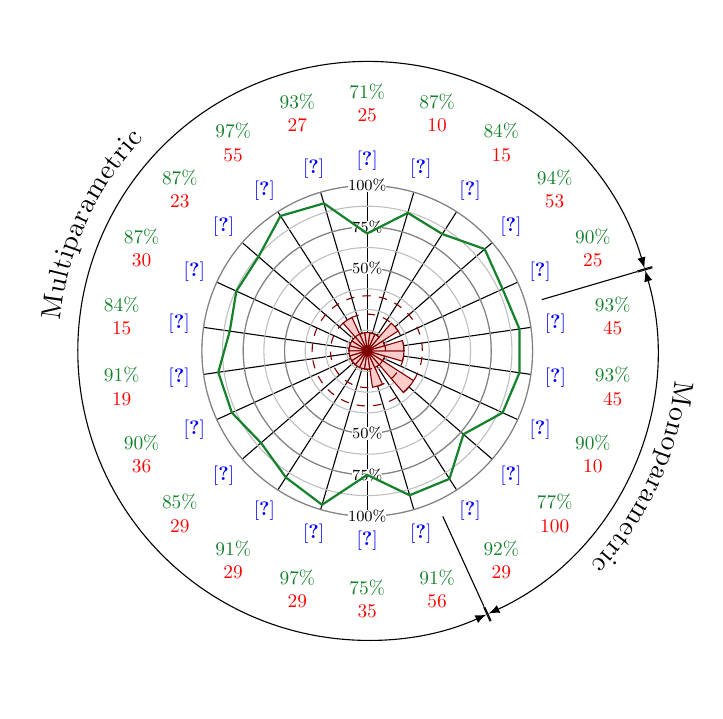
\begin{tikzpicture}[scale=.7,every node/.style={scale=0.7}]

      \def\labels{
        {\color{blue}\cite{Ampeliotis2008}},
        {\color{blue}\cite{Antic2013}},
        {\color{blue}\cite{Chan2003}},
        {\color{blue}\cite{Giannini2013}},
        {\color{blue}\cite{Langer2009}},
        {\color{blue}\cite{Lopes2011}},
        {\color{blue}\cite{Lv2009}},
        {\color{blue}\cite{Niaf2011}},
        {\color{blue}\cite{Niaf2012}},
        {\color{blue}\cite{Tiwari2009a}},
        {\color{blue}\cite{Tiwari2010}},
        {\color{blue}\cite{Tiwari2012}},
        {\color{blue}\cite{Tiwari2013}},
        {\color{blue}\cite{Vos2008}},
        {\color{blue}\cite{Vos2010}},
        {\color{blue}\cite{lehaire2014computer}},
        {\color{blue}\cite{giannini2015fully}},
        {\color{blue}\cite{Mazzetti2011}},
        {\color{blue}\cite{Puech2009}},
        {\color{blue}\cite{Vos2008a}},
        {\color{blue}\cite{rampun2016computerb}},
        {\color{blue}\cite{rampun2016computer}} 
      }

      \def\reward{90,94,84,87,71,93,97,87,87,84,91,90,85,91,97,75,91,92,77,90,93,93}
      \def\dbSize{25,53,15,10,25,27,55,23,30,15,19,36,29,29,29,35,56,29,100,10,45,45}
      \def\dbClass{1,2,1,1,1,1,2,1,1,1,1,1,1,1,1,1,2,1,3,1,2,2}
      \def\cZoom{3} 
      \def\percentageLabelAngle{90}
      \def\nbeams{22}
      \pgfmathsetmacro\beamAngle{(360/\nbeams)}
      \pgfmathsetmacro\halfAngle{(180/\nbeams)}
      \pgfmathsetmacro\globalRotation{\halfAngle}

      % draw the radiants
      \foreach \n  [count=\ni] in \labels
      {
        \pgfmathsetmacro\cAngle{{(\ni*(360/\nbeams))+\globalRotation}}
        \draw(\cAngle:{\cZoom*1.15})  node[fill=white] {\n};
        \draw [thin] (0,0) -- (\cAngle:{\cZoom*1}) ;

      }

      % draw the % rings 
      \foreach \x in {12.5,25, ...,100} 
      \draw [thin,color=gray!50] (0,0) circle [radius={\cZoom*\x/100}];

      \foreach \x in {50,75,100}
      { 
        \draw [thin,color=black!50] (0,0) circle [radius={\cZoom/100*\x}];
        \foreach \a in {0, 180} \draw ({\percentageLabelAngle+\a}:{\cZoom*0.01*\x}) node  [inner sep=0pt,outer sep=0pt,fill=white,font=\fontsize{8}{8.5}\selectfont]{$\x\%$};
      }

      % draw the path of the percentages
      \def\aux{{\reward}}
      \pgfmathsetmacro\origin{\aux[\nbeams-1]} 
      \draw [semiAuto, thick] (\globalRotation:{\cZoom*\origin/100}) \foreach \n  [count=\ni] in \reward { -- ({(\ni*(360/\nbeams))+\globalRotation}:{\cZoom*\n/100}) } ;

      % label all the percentags
      \foreach \n [count=\ni] in \dbSize 
      {
        \pgfmathsetmacro\cAngle{{(\ni*(360/\nbeams))+\globalRotation}}
        \pgfmathsetmacro\nreward{\aux[\ni-1]}
        \draw (\cAngle:{\cZoom*1.5}) node[align=center] {{\color{semiAuto}\nreward $\%$} \\ {\color{red}\n} };
      } ;

      % draw the database rose
      \def\dbScale{\9}
      \foreach \n [count=\ni] in \dbClass
      \filldraw[fill=red!20!white, draw=red!50!black]
      (0,0) -- ({\ni*(360/\nbeams)-\halfAngle+\globalRotation}:{\cZoom*\n/9}) arc ({\ni*(360/\nbeams)-\halfAngle+\globalRotation}:{\ni*(360/\nbeams)+\halfAngle+\globalRotation}:{\cZoom*\n/9}) -- cycle;
      \foreach \x in {1,2,3}
      \draw [thin,color=red!50!black,dashed] (0,0) circle [radius={\cZoom*\x/9}];

      %% draw the domain of each class 
      \def\puta{17/0/{Multiparametric},
        5/17/{Monoparametric}}

      \foreach \numElm/\contadorQueNoSeCalcular/\name [count=\ni] in \puta
      {

        \pgfmathsetmacro\initialAngle{(\contadorQueNoSeCalcular*\beamAngle)+\halfAngle+\globalRotation}
        \pgfmathsetmacro\finalAngle  {((\numElm+\contadorQueNoSeCalcular)*\beamAngle)+\halfAngle+\globalRotation}
        \pgfmathsetmacro\l  {\cZoom*1.65+.3pt}
        \draw (\initialAngle:{\cZoom*1.7}) -- (\initialAngle:{\cZoom*1.1});
        \draw [ |<->|,>=latex] (\initialAngle:\l) arc (\initialAngle:\finalAngle:\l) ;     
        \pgfmathsetmacro\r  {\cZoom*1.65+.45pt}
        {\draw [decoration={raise=4pt,text along path,text={\name},text align={center}},decorate] (\finalAngle:\r) arc (\finalAngle:\initialAngle:\r);}
      }
      
    \end{tikzpicture}}\\
  \subfigure[]{
    \label{fig:auc30}
    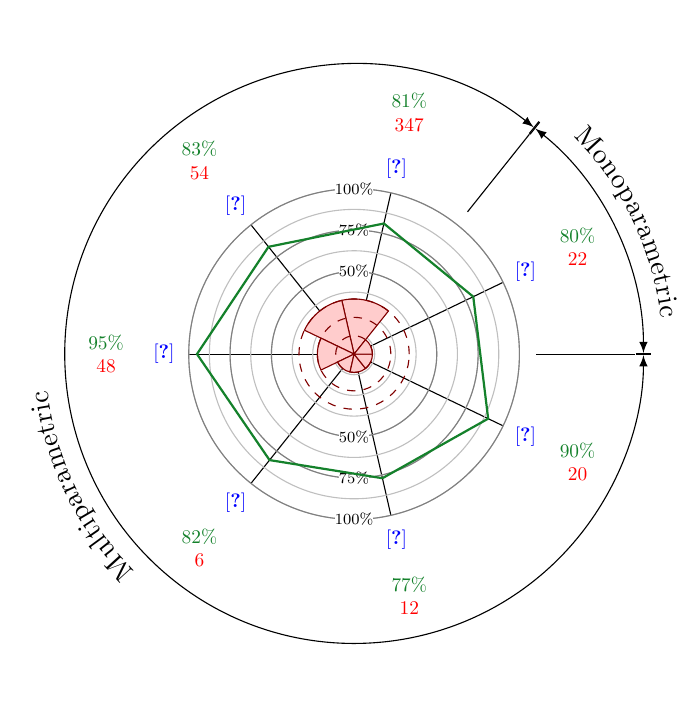
\begin{tikzpicture}[scale=.7,every node/.style={scale=0.7}]

      \def\labels{
        {\color{blue}\cite{Litjens2014}},
        {\color{blue}\cite{Liu2013}},
        {\color{blue}\cite{Peng2013}},
        {\color{blue}\cite{Viswanath2009}},
        {\color{blue}\cite{Viswanath2011}},
        {\color{blue}\cite{khalvati2015automated}},
        {\color{blue}\cite{Viswanath2012}}
      }

      \def\reward{81,83,95,82,77,90,80}
      \def\dbSize{347,54,48,6,12,20,22}
      \def\dbClass{3,3,2,1,1,1,1}
      \def\cZoom{3} 
      \def\percentageLabelAngle{90}
      \def\nbeams{7}
      \pgfmathsetmacro\beamAngle{(360/\nbeams)}
      \pgfmathsetmacro\halfAngle{(180/\nbeams)}
      \pgfmathsetmacro\globalRotation{\halfAngle}

      % draw the radiants
      \foreach \n  [count=\ni] in \labels
      {
        \pgfmathsetmacro\cAngle{{(\ni*(360/\nbeams))+\globalRotation}}
        \draw(\cAngle:{\cZoom*1.15})  node[fill=white] {\n};
        \draw [thin] (0,0) -- (\cAngle:{\cZoom*1}) ;

      }

      % draw the % rings 
      \foreach \x in {12.5,25, ...,100} 
      \draw [thin,color=gray!50] (0,0) circle [radius={\cZoom*\x/100}];

      \foreach \x in {50,75,100}
      { 
        \draw [thin,color=black!50] (0,0) circle [radius={\cZoom/100*\x}];
        \foreach \a in {0, 180} \draw ({\percentageLabelAngle+\a}:{\cZoom*0.01*\x}) node  [inner sep=0pt,outer sep=0pt,fill=white,font=\fontsize{8}{8.5}\selectfont]{$\x\%$};
      }

      % draw the path of the percentages
      \def\aux{{\reward}}
      \pgfmathsetmacro\origin{\aux[\nbeams-1]} 
      \draw [semiAuto, thick] (\globalRotation:{\cZoom*\origin/100}) \foreach \n  [count=\ni] in \reward { -- ({(\ni*(360/\nbeams))+\globalRotation}:{\cZoom*\n/100}) } ;

      % label all the percentags
      \foreach \n [count=\ni] in \dbSize 
      {
        \pgfmathsetmacro\cAngle{{(\ni*(360/\nbeams))+\globalRotation}}
        \pgfmathsetmacro\nreward{\aux[\ni-1]}
        \draw (\cAngle:{\cZoom*1.5}) node[align=center] {{\color{semiAuto}\nreward $\%$} \\ {\color{red}\n} };
      } ;

      % draw the database rose
      \def\dbScale{\9}
      \foreach \n [count=\ni] in \dbClass
      \filldraw[fill=red!20!white, draw=red!50!black]
      (0,0) -- ({\ni*(360/\nbeams)-\halfAngle+\globalRotation}:{\cZoom*\n/9}) arc ({\ni*(360/\nbeams)-\halfAngle+\globalRotation}:{\ni*(360/\nbeams)+\halfAngle+\globalRotation}:{\cZoom*\n/9}) -- cycle;
      \foreach \x in {1,2,3}
      \draw [thin,color=red!50!black,dashed] (0,0) circle [radius={\cZoom*\x/9}];

      %% draw the domain of each class 
      \def\puta{6/0/{Multiparametric},
        1/6/{Monoparametric}}

      \foreach \numElm/\contadorQueNoSeCalcular/\name [count=\ni] in \puta
      {

        \pgfmathsetmacro\initialAngle{(\contadorQueNoSeCalcular*\beamAngle)+\halfAngle+\globalRotation}
        \pgfmathsetmacro\finalAngle  {((\numElm+\contadorQueNoSeCalcular)*\beamAngle)+\halfAngle+\globalRotation}
        \pgfmathsetmacro\l  {\cZoom*1.65+.3pt}
        \draw (\initialAngle:{\cZoom*1.7}) -- (\initialAngle:{\cZoom*1.1});
        \draw [ |<->|,>=latex] (\initialAngle:\l) arc (\initialAngle:\finalAngle:\l) ;     
        \pgfmathsetmacro\r  {\cZoom*1.65+.45pt}
        {\draw [decoration={raise=4pt,text along path,  text={\name},text align={center}},decorate] (\finalAngle:\r) arc (\finalAngle:\initialAngle:\r);}
      }
      
    \end{tikzpicture}
 }
  %\hspace{\fill}
  \caption[Results comparison from the state-of-the-art in terms of \acs*{auc}.]{Numerical and graphical comparison of the results in terms of \acs*{auc} for \SI{1.5}{\tesla} and \SI{3}{\tesla} \acs*{mri} scanners. The {\color{semiAuto}green} value represents the metric and are graphically reported in the {\color{semiAuto}green} curve in the center of the figure. The {\color{red}red} value and areas correspond to the number of patients in the dataset. The numbers between brackets in {blue\color{blue}} correspond to the reference as reported in \acs{tab}~\ref{tab:sumpap}.}
  \label{fig:auc}
\end{figure}


\begin{figure}%
 \centering
 \hspace*{\fill}
  \subfigure[]{
    \label{fig:sens15}
    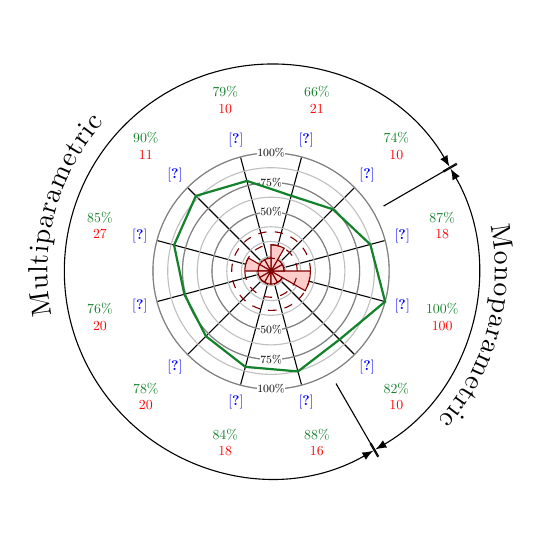
\begin{tikzpicture}[scale=.5,every node/.style={scale=0.5}]

      \def\labels{
        {\color{blue}\cite{Artan2009}},
        {\color{blue}\cite{Artan2010}},
        {\color{blue}\cite{Giannini2013}},
        {\color{blue}\cite{Liu2009}},
        {\color{blue}\cite{Lopes2011}},
        {\color{blue}\cite{Ozer2009}},
        {\color{blue}\cite{Ozer2010}},
        {\color{blue}\cite{Tiwari2009a}},
        {\color{blue}\cite{Viswanath2008}},
        {\color{blue}\cite{Mazzetti2011}},
        {\color{blue}\cite{Puech2009}},
        {\color{blue}\cite{Tiwari2008}}
      }

      \def\reward{74,66,79,90,85,76,78,84,88,82,100,87}
      \def\dbSize{10,21,10,11,27,20,20,18,16,10,100,18}
      \def\dbClass{1,2,1,1,2,1,1,1,1,1,3,1}
      \def\cZoom{3} 
      \def\percentageLabelAngle{90}
      \def\nbeams{12}
      \pgfmathsetmacro\beamAngle{(360/\nbeams)}
      \pgfmathsetmacro\halfAngle{(180/\nbeams)}
      \pgfmathsetmacro\globalRotation{\halfAngle}

      % draw the radiants
      \foreach \n  [count=\ni] in \labels
      {
        \pgfmathsetmacro\cAngle{{(\ni*(360/\nbeams))+\globalRotation}}
        \draw(\cAngle:{\cZoom*1.15})  node[fill=white] {\n};
        \draw [thin] (0,0) -- (\cAngle:{\cZoom*1}) ;

      }

      % draw the % rings 
      \foreach \x in {12.5,25, ...,100} 
      \draw [thin,color=gray!50] (0,0) circle [radius={\cZoom*\x/100}];

      \foreach \x in {50,75,100}
      { 
        \draw [thin,color=black!50] (0,0) circle [radius={\cZoom/100*\x}];
        \foreach \a in {0, 180} \draw ({\percentageLabelAngle+\a}:{\cZoom*0.01*\x}) node  [inner sep=0pt,outer sep=0pt,fill=white,font=\fontsize{8}{8.5}\selectfont]{$\x\%$};
      }

      % draw the path of the percentages
      \def\aux{{\reward}}
      \pgfmathsetmacro\origin{\aux[\nbeams-1]} 
      \draw [semiAuto, thick] (\globalRotation:{\cZoom*\origin/100}) \foreach \n  [count=\ni] in \reward { -- ({(\ni*(360/\nbeams))+\globalRotation}:{\cZoom*\n/100}) } ;

      % label all the percentags
      \foreach \n [count=\ni] in \dbSize 
      {
        \pgfmathsetmacro\cAngle{{(\ni*(360/\nbeams))+\globalRotation}}
        \pgfmathsetmacro\nreward{\aux[\ni-1]}
        \draw (\cAngle:{\cZoom*1.5}) node[align=center] {{\color{semiAuto}\nreward $\%$} \\ {\color{red}\n} };
      } ;

      % draw the database rose
      \def\dbScale{\9}
      \foreach \n [count=\ni] in \dbClass
      \filldraw[fill=red!20!white, draw=red!50!black]
      (0,0) -- ({\ni*(360/\nbeams)-\halfAngle+\globalRotation}:{\cZoom*\n/9}) arc ({\ni*(360/\nbeams)-\halfAngle+\globalRotation}:{\ni*(360/\nbeams)+\halfAngle+\globalRotation}:{\cZoom*\n/9}) -- cycle;
      \foreach \x in {1,2,3}
      \draw [thin,color=red!50!black,dashed] (0,0) circle [radius={\cZoom*\x/9}];

      %% draw the domain of each class 
      \def\puta{9/0/{Multiparametric},
        3/9/{Monoparametric}}

      \foreach \numElm/\contadorQueNoSeCalcular/\name [count=\ni] in \puta
      {

        \pgfmathsetmacro\initialAngle{(\contadorQueNoSeCalcular*\beamAngle)+\halfAngle+\globalRotation}
        \pgfmathsetmacro\finalAngle  {((\numElm+\contadorQueNoSeCalcular)*\beamAngle)+\halfAngle+\globalRotation}
        \pgfmathsetmacro\l  {\cZoom*1.65+.3pt}
        \draw (\initialAngle:{\cZoom*1.7}) -- (\initialAngle:{\cZoom*1.1});
        \draw [ |<->|,>=latex] (\initialAngle:\l) arc (\initialAngle:\finalAngle:\l) ;     
        \pgfmathsetmacro\r  {\cZoom*1.65+.45pt}
        {\draw [decoration={raise=4pt,text along path,  text={\name},text align={center}},decorate] (\finalAngle:\r) arc (\finalAngle:\initialAngle:\r);}
      }
      
    \end{tikzpicture}
}\hfill
  \subfigure[]{
    \label{fig:spec15}
    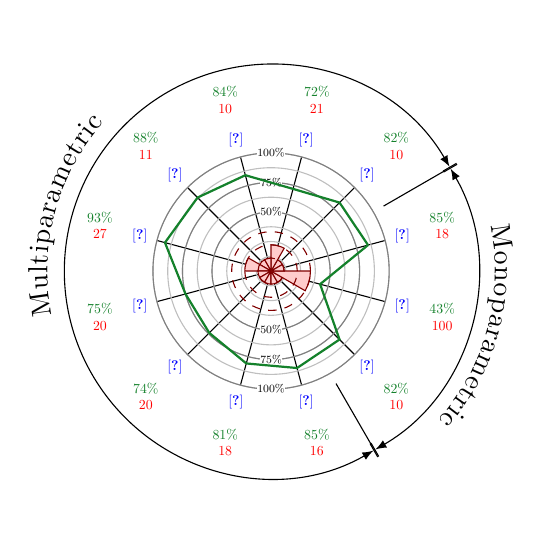
\begin{tikzpicture}[scale=.5,every node/.style={scale=0.5}]

      \def\labels{
        {\color{blue}\cite{Artan2009}},
        {\color{blue}\cite{Artan2010}},
        {\color{blue}\cite{Giannini2013}},
        {\color{blue}\cite{Liu2009}},
        {\color{blue}\cite{Lopes2011}},
        {\color{blue}\cite{Ozer2009}},
        {\color{blue}\cite{Ozer2010}},
        {\color{blue}\cite{Tiwari2009a}},
        {\color{blue}\cite{Viswanath2008}},
        {\color{blue}\cite{Mazzetti2011}},
        {\color{blue}\cite{Puech2009}},
        {\color{blue}\cite{Tiwari2008}}
      }

      \def\reward{82,72,84,88,93,75,74,81,85,82,43,85}
      \def\dbSize{10,21,10,11,27,20,20,18,16,10,100,18}
      \def\dbClass{1,2,1,1,2,1,1,1,1,1,3,1}
      \def\cZoom{3} 
      \def\percentageLabelAngle{90}
      \def\nbeams{12}
      \pgfmathsetmacro\beamAngle{(360/\nbeams)}
      \pgfmathsetmacro\halfAngle{(180/\nbeams)}
      \pgfmathsetmacro\globalRotation{\halfAngle}

      % draw the radiants
      \foreach \n  [count=\ni] in \labels
      {
        \pgfmathsetmacro\cAngle{{(\ni*(360/\nbeams))+\globalRotation}}
        \draw(\cAngle:{\cZoom*1.15})  node[fill=white] {\n};
        \draw [thin] (0,0) -- (\cAngle:{\cZoom*1}) ;

      }

      % draw the % rings 
      \foreach \x in {12.5,25, ...,100} 
      \draw [thin,color=gray!50] (0,0) circle [radius={\cZoom*\x/100}];

      \foreach \x in {50,75,100}
      { 
        \draw [thin,color=black!50] (0,0) circle [radius={\cZoom/100*\x}];
        \foreach \a in {0, 180} \draw ({\percentageLabelAngle+\a}:{\cZoom*0.01*\x}) node  [inner sep=0pt,outer sep=0pt,fill=white,font=\fontsize{8}{8.5}\selectfont]{$\x\%$};
      }

      % draw the path of the percentages
      \def\aux{{\reward}}
      \pgfmathsetmacro\origin{\aux[\nbeams-1]} 
      \draw [semiAuto, thick] (\globalRotation:{\cZoom*\origin/100}) \foreach \n  [count=\ni] in \reward { -- ({(\ni*(360/\nbeams))+\globalRotation}:{\cZoom*\n/100}) } ;

      % label all the percentags
      \foreach \n [count=\ni] in \dbSize 
      {
        \pgfmathsetmacro\cAngle{{(\ni*(360/\nbeams))+\globalRotation}}
        \pgfmathsetmacro\nreward{\aux[\ni-1]}
        \draw (\cAngle:{\cZoom*1.5}) node[align=center] {{\color{semiAuto}\nreward $\%$} \\ {\color{red}\n} };
      } ;

      % draw the database rose
      \def\dbScale{\9}
      \foreach \n [count=\ni] in \dbClass
      \filldraw[fill=red!20!white, draw=red!50!black]
      (0,0) -- ({\ni*(360/\nbeams)-\halfAngle+\globalRotation}:{\cZoom*\n/9}) arc ({\ni*(360/\nbeams)-\halfAngle+\globalRotation}:{\ni*(360/\nbeams)+\halfAngle+\globalRotation}:{\cZoom*\n/9}) -- cycle;
      \foreach \x in {1,2,3}
      \draw [thin,color=red!50!black,dashed] (0,0) circle [radius={\cZoom*\x/9}];

      %% draw the domain of each class 
      \def\puta{9/0/{Multiparametric},
        3/9/{Monoparametric}}

      \foreach \numElm/\contadorQueNoSeCalcular/\name [count=\ni] in \puta
      {

        \pgfmathsetmacro\initialAngle{(\contadorQueNoSeCalcular*\beamAngle)+\halfAngle+\globalRotation}
        \pgfmathsetmacro\finalAngle  {((\numElm+\contadorQueNoSeCalcular)*\beamAngle)+\halfAngle+\globalRotation}
        \pgfmathsetmacro\l  {\cZoom*1.65+.3pt}
        \draw (\initialAngle:{\cZoom*1.7}) -- (\initialAngle:{\cZoom*1.1});
        \draw [ |<->|,>=latex] (\initialAngle:\l) arc (\initialAngle:\finalAngle:\l) ;     
        \pgfmathsetmacro\r  {\cZoom*1.65+.45pt}
        {\draw [decoration={raise=4pt,text along path,  text={\name},text align={center}},decorate] (\finalAngle:\r) arc (\finalAngle:\initialAngle:\r);}
      }
      
    \end{tikzpicture}
  }\hspace*{\fill}
  \\
  \hspace*{\fill}
  \subfigure[]{
    \label{fig:sens30}
    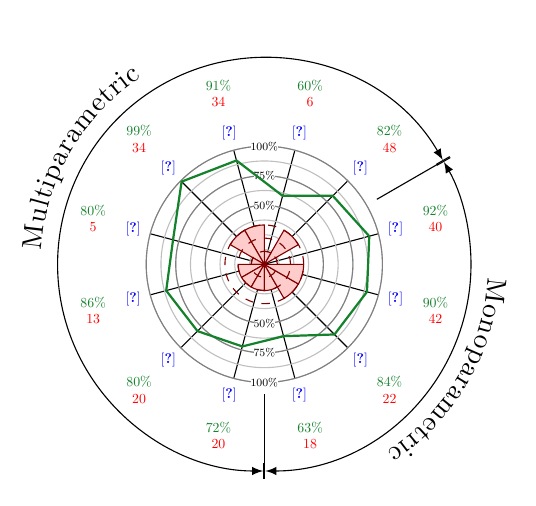
\begin{tikzpicture}[scale=.5,every node/.style={scale=0.5}]

      \def\labels{
        {\color{blue}\cite{Peng2013}},
        {\color{blue}\cite{Viswanath2008a}},
        {\color{blue}\cite{trigui2017automatic}},
        {\color{blue}\cite{trigui2016classification}},
        {\color{blue}\cite{cameron2014multiparametric}},
        {\color{blue}\cite{cameron2016maps}},
        {\color{blue}\cite{khalvati2015automated}},
        {\color{blue}\cite{chung2015prostate}},
        {\color{blue}\cite{Matulewicz2013}},
        {\color{blue}\cite{Parfait2012}},
        {\color{blue}\cite{Sung2011}},
        {\color{blue}\cite{samarasinghe2016semi}}
      }

      \def\reward{82,60,91,99,80,86,80,72,63,84,90,92}
      \def\dbSize{48,6,34,34,5,13,20,20,18,22,42,40}
      \def\dbClass{3,1,3,3,1,2,2,2,2,3,3}
      \def\cZoom{3} 
      \def\percentageLabelAngle{90}
      \def\nbeams{12}
      \pgfmathsetmacro\beamAngle{(360/\nbeams)}
      \pgfmathsetmacro\halfAngle{(180/\nbeams)}
      \pgfmathsetmacro\globalRotation{\halfAngle}


      % draw the radiants
      \foreach \n  [count=\ni] in \labels
      {
        \pgfmathsetmacro\cAngle{{(\ni*(360/\nbeams))+\globalRotation}}
        \draw(\cAngle:{\cZoom*1.15})  node[fill=white] {\n};
        \draw [thin] (0,0) -- (\cAngle:{\cZoom*1}) ;

      }

      % draw the % rings 
      \foreach \x in {12.5,25, ...,100} 
      \draw [thin,color=gray!50] (0,0) circle [radius={\cZoom*\x/100}];

      \foreach \x in {50,75,100}
      { 
        \draw [thin,color=black!50] (0,0) circle [radius={\cZoom/100*\x}];
        \foreach \a in {0, 180} \draw ({\percentageLabelAngle+\a}:{\cZoom*0.01*\x}) node  [inner sep=0pt,outer sep=0pt,fill=white,font=\fontsize{8}{8.5}\selectfont]{$\x\%$};
      }

      % draw the path of the percentages
      \def\aux{{\reward}}
      \pgfmathsetmacro\origin{\aux[\nbeams-1]} 
      \draw [semiAuto, thick] (\globalRotation:{\cZoom*\origin/100}) \foreach \n  [count=\ni] in \reward { -- ({(\ni*(360/\nbeams))+\globalRotation}:{\cZoom*\n/100}) } ;

      % label all the percentags
      \foreach \n [count=\ni] in \dbSize 
      {
        \pgfmathsetmacro\cAngle{{(\ni*(360/\nbeams))+\globalRotation}}
        \pgfmathsetmacro\nreward{\aux[\ni-1]}
        \draw (\cAngle:{\cZoom*1.5}) node[align=center] {{\color{semiAuto}\nreward $\%$} \\ {\color{red}\n} };
      } ;

      % draw the database rose
      \def\dbScale{\9}
      \foreach \n [count=\ni] in \dbClass
      \filldraw[fill=red!20!white, draw=red!50!black]
      (0,0) -- ({\ni*(360/\nbeams)-\halfAngle+\globalRotation}:{\cZoom*\n/9}) arc ({\ni*(360/\nbeams)-\halfAngle+\globalRotation}:{\ni*(360/\nbeams)+\halfAngle+\globalRotation}:{\cZoom*\n/9}) -- cycle;
      \foreach \x in {1,2,3}
      \draw [thin,color=red!50!black,dashed] (0,0) circle [radius={\cZoom*\x/9}];

      %% draw the domain of each class 
      \def\puta{8/0/{Multiparametric},
        4/8/{Monoparametric}}

      \foreach \numElm/\contadorQueNoSeCalcular/\name [count=\ni] in \puta
      {

        \pgfmathsetmacro\initialAngle{(\contadorQueNoSeCalcular*\beamAngle)+\halfAngle+\globalRotation}
        \pgfmathsetmacro\finalAngle  {((\numElm+\contadorQueNoSeCalcular)*\beamAngle)+\halfAngle+\globalRotation}
        \pgfmathsetmacro\l  {\cZoom*1.65+.3pt}
        \draw (\initialAngle:{\cZoom*1.7}) -- (\initialAngle:{\cZoom*1.1});
        \draw [ |<->|,>=latex] (\initialAngle:\l) arc (\initialAngle:\finalAngle:\l) ;     
        \pgfmathsetmacro\r  {\cZoom*1.65+.45pt}
        {\draw [decoration={raise=4pt,text along path,  text={\name},text align={center}},decorate] (\finalAngle:\r) arc (\finalAngle:\initialAngle:\r);}
      }
      
    \end{tikzpicture}
}\hfill
  \subfigure[]{
    \label{fig:spec30}
    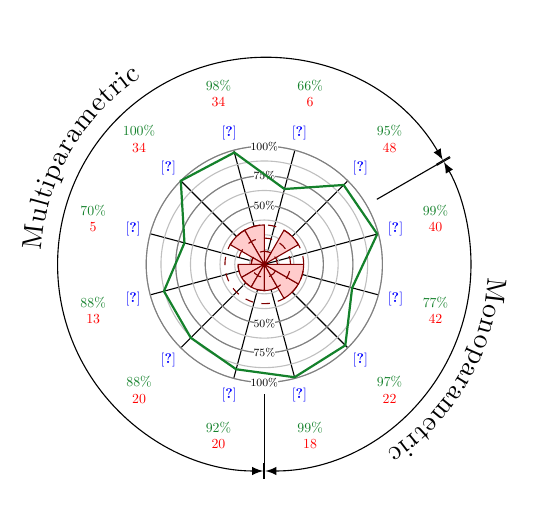
\begin{tikzpicture}[scale=.5,every node/.style={scale=0.5}]

      \def\labels{
        {\color{blue}\cite{Peng2013}},
        {\color{blue}\cite{Viswanath2008a}},
        {\color{blue}\cite{trigui2017automatic}},
        {\color{blue}\cite{trigui2016classification}},
        {\color{blue}\cite{cameron2014multiparametric}},
        {\color{blue}\cite{cameron2016maps}},
        {\color{blue}\cite{khalvati2015automated}},
        {\color{blue}\cite{chung2015prostate}},
        {\color{blue}\cite{Matulewicz2013}},
        {\color{blue}\cite{Parfait2012}},
        {\color{blue}\cite{Sung2011}},
        {\color{blue}\cite{samarasinghe2016semi}}
      }

      \def\reward{95,66,98,100,70,88,88,92,99,97,77,99}
      \def\dbSize{48,6,34,34,5,13,20,20,18,22,42,40}
      \def\dbClass{3,1,3,3,1,2,2,2,2,3,3}
            
      \def\cZoom{3} 
      \def\percentageLabelAngle{90}
      \def\nbeams{12}
      \pgfmathsetmacro\beamAngle{(360/\nbeams)}
      \pgfmathsetmacro\halfAngle{(180/\nbeams)}
      \pgfmathsetmacro\globalRotation{\halfAngle}

      % draw the radiants
      \foreach \n  [count=\ni] in \labels
      {
        \pgfmathsetmacro\cAngle{{(\ni*(360/\nbeams))+\globalRotation}}
        \draw(\cAngle:{\cZoom*1.15})  node[fill=white] {\n};
        \draw [thin] (0,0) -- (\cAngle:{\cZoom*1}) ;

      }

      % draw the % rings 
      \foreach \x in {12.5,25, ...,100} 
      \draw [thin,color=gray!50] (0,0) circle [radius={\cZoom*\x/100}];

      \foreach \x in {50,75,100}
      { 
        \draw [thin,color=black!50] (0,0) circle [radius={\cZoom/100*\x}];
        \foreach \a in {0, 180} \draw ({\percentageLabelAngle+\a}:{\cZoom*0.01*\x}) node  [inner sep=0pt,outer sep=0pt,fill=white,font=\fontsize{8}{8.5}\selectfont]{$\x\%$};
      }

      % draw the path of the percentages
      \def\aux{{\reward}}
      \pgfmathsetmacro\origin{\aux[\nbeams-1]} 
      \draw [semiAuto, thick] (\globalRotation:{\cZoom*\origin/100}) \foreach \n  [count=\ni] in \reward { -- ({(\ni*(360/\nbeams))+\globalRotation}:{\cZoom*\n/100}) } ;

      % label all the percentags
      \foreach \n [count=\ni] in \dbSize 
      {
        \pgfmathsetmacro\cAngle{{(\ni*(360/\nbeams))+\globalRotation}}
        \pgfmathsetmacro\nreward{\aux[\ni-1]}
        \draw (\cAngle:{\cZoom*1.5}) node[align=center] {{\color{semiAuto}\nreward $\%$} \\ {\color{red}\n} };
      } ;

      % draw the database rose
      \def\dbScale{\9}
      \foreach \n [count=\ni] in \dbClass
      \filldraw[fill=red!20!white, draw=red!50!black]
      (0,0) -- ({\ni*(360/\nbeams)-\halfAngle+\globalRotation}:{\cZoom*\n/9}) arc ({\ni*(360/\nbeams)-\halfAngle+\globalRotation}:{\ni*(360/\nbeams)+\halfAngle+\globalRotation}:{\cZoom*\n/9}) -- cycle;
      \foreach \x in {1,2,3}
      \draw [thin,color=red!50!black,dashed] (0,0) circle [radius={\cZoom*\x/9}];

      %% draw the domain of each class 
      \def\puta{8/0/{Multiparametric},
        4/8/{Monoparametric}}

      \foreach \numElm/\contadorQueNoSeCalcular/\name [count=\ni] in \puta
      {

        \pgfmathsetmacro\initialAngle{(\contadorQueNoSeCalcular*\beamAngle)+\halfAngle+\globalRotation}
        \pgfmathsetmacro\finalAngle  {((\numElm+\contadorQueNoSeCalcular)*\beamAngle)+\halfAngle+\globalRotation}
        \pgfmathsetmacro\l  {\cZoom*1.65+.3pt}
        \draw (\initialAngle:{\cZoom*1.7}) -- (\initialAngle:{\cZoom*1.1});
        \draw [ |<->|,>=latex] (\initialAngle:\l) arc (\initialAngle:\finalAngle:\l) ;     
        \pgfmathsetmacro\r  {\cZoom*1.65+.45pt}
        {\draw [decoration={raise=4pt,text along path,  text={\name},text align={center}},decorate] (\finalAngle:\r) arc (\finalAngle:\initialAngle:\r);}
      }
      
    \end{tikzpicture}
  }
  \hspace*{\fill}
  \caption[Comparison of the state-of-the-art results in terms of \acs*{se} and \acs*{sp}.]{Numerical and graphical comparison of the results in terms of \acs*{se}~\subref{fig:sens15},~\subref{fig:sens30} and \acs*{sp}~\subref{fig:spec15},~\subref{fig:spec30} for \SI{1.5}{\tesla} and \SI{3}{\tesla} \ac{mri} scanners. The value in {\color{semiAuto}green} represents the metric and are graphically reported in the {\color{semiAuto}green} curve in the center of the figure. The {\color{red}red} value and areas correspond to the number of patients in the dataset. The numbers between brackets in {\color{blue}blue} correspond to the reference as reported in \acs{tab}~\ref{tab:sumpap}.}
  \label{fig:sensspec}
\end{figure}


\subsection{Comparison}\label{subsec:chp3:dis:com}

We would like to stress the following findings drawn during the review of the different studies:

\begin{enumerate}
\item Quantitatively, it is difficult to make a fair comparison between the different studies reviewed.
Different factors come into play to elucidate this fact.
Mainly a lack of standardization has to be pointed out in regard to experimental evaluation:
(i) different datasets are used during the evaluation of the frameworks developed hindering an inter-study comparison.
The same conclusion has been recently drawn by~\cite{Litjens2014} supporting this argument;
(ii) the experimental results are not reported with a common metric which leads to the inability to compare the different studies.

\item \label{here} However, multiple studies reported some performance improvements using \ac{mpmri} techniques instead of mono-parametric imaging techniques.
Considering only the most recent studies proposing \ac{cade}-\ac{cadx} frameworks, the following results can be highlighted.
\citeauthor{Viswanath2011} obtained an \ac{auc} of \SI{77}{\percent} using an ensemble learning approach combining the features from the three \ac{mri} modalities --- i.e., \ac{t2w}-\ac{mri}, \ac{dce}--\ac{mri}, and \ac{dw}-\ac{mri}, while the results obtained as standalone modality range from \SIrange{62}{65}{\percent}~\cite{Viswanath2011}. 
\citeauthor{Tiwari2013} drawn similar conclusions by using \ac{t2w}-\ac{mri} and \ac{mrsi} modalities as both in standalone and multi-parametric frameworks with an improved \ac{auc} ranging from \SI{57}{\percent}-\SIrange{76}{85}{\percent}~\cite{Tiwari2013}.
The most recent work of \citeauthor{Litjens2014} obtained an improved \ac{auc} metric from \SI{71}{\percent}-\SI{76}{\percent} considering each modality separately --- i.e., \ac{t2w}-\ac{mri}, \ac{dce}-\ac{mri}, and \ac{dw}-\ac{mri} --- to \SI{89}{\percent} in their \ac{mpmri} framework.

\item The studies comparing particular combination of more than a single modality give rise to the same fact~\cite{Ozer2010,Litjens2011,Liu2013,Litjens2014}: using 3 modalities lead to better performances than using any combination of 2 modalities. 

\item Unlike the previous remark~\ref{here}, no straightforward conclusions can be given regarding the classification performance using each modality in a standalone framework.
The modality being processed by different methods, it does not allow us to conclude if a modality by itself is more suited than another.
However, we are able to distinguish some interesting trends which deserve the attention of the community.
\citeauthor{Tiwari2013} in~\cite{Tiwari2009a,Tiwari2012,Tiwari2013} observed that \ac{mrsi} is a more suitable modality than \ac{t2w} to highlight \ac{cap}.
Moreover, \ac{adc} maps have shown a better discriminative power than \ac{t2w} as well~\cite{Langer2009,Viswanath2011,Peng2013}.
Lately, \citeauthor{Litjens2014} observed that \ac{dw}-\ac{mri} modality is more suitable than both \ac{dce}-\ac{mri} and \ac{t2w}-\ac{mri} to distinguish \ac{cap} in their \ac{cadx} system~\cite{Litjens2014}. 
Recently, \citeauthor{rampun2016computerb} showed, however, some promising results using \ac{t2w}-\ac{mri} only in conjunction with textons and \ac{bow}; this study should be transposed to other \ac{mri} modalities~\cite{rampun2016computerb}.

\item Furthermore, \ac{mpmri} has attracted the attention of both radiologists and computer vision researchers.
Indeed, pioneer research groups included new modalities over years when at the same time, new research groups directly introduced \ac{mpmri} \ac{cad} systems.
These facts lead us to think that \ac{cap} researches will benefit from \ac{mpmri} techniques.

\item When focusing on the different modalities used, it can be pointed out that only \citeauthor{trigui2017automatic} reported the use of all modalities in a single framework by incorporating the \ac{mrsi} modality~\cite{trigui2016classification,trigui2017automatic}.
Although the results reported are promising, the detection has been performed at \ac{mrsi} scale and further investigations need to be carried out.
Nevertheless, \ac{mrsi} has shown some overall good classification performance at the price of a lower resolution as well as an increased acquisition time.
Moreover, \ac{mrsi} analysis is more complex in comparison with the other modalities.
To our mind, \ac{mrsi} could contribute in a \ac{mpmri} framework and should be fused with the other modalities.

\item Lately, 3 studies focused on developing a region-based classification in which \ac{pz} and \ac{cg} will be analyzed separately~\cite{Viswanath2012,Litjens2012,Litjens2014}.
The promising obtained results indicate that this strategy should be further investigated.

\item Recent studies are using quantitative features in addition to \ac{si}.
It seems that these quantitative features provide uncorrelated information with respect to \ac{si} features and should lead to better classification performance when combined all together. 

\item Regarding the methods used in the ``image regularization'' --- i.e., pre-processing, segmentation, and registration --- it is particularly difficult to distinguish the benefit of a method over another since none of the studies focus on making comparison of these processing stages.
The focus is usually entirely based on the ``image classification'' framework where different methods are directly compared.
Note that the performance of a classifier is highly linked with the features vector extracted from particular data.
Hence, one can not conclude that a machine learning method is more appropriate than another, but we can identify a trend in which \ac{svm} as well as ensemble learning classifiers --- i.e., AdaBoost, GentleBoost, and \ac{rf} --- seem to perform better than neural network, \ac{lda}, or Naive Bayes.

\item We would like to draw the attention of the reader on the feature extraction/selection stage.
This processing could reduce the complexity and also allow to find a better feature space for classification.
However, few studies are performing such approaches.
\citeauthor{Niaf2012}, \citeauthor{khalvati2015automated}, \citeauthor{chung2015prostate}, and \citeauthor{rampun2016computer} are successfully applying a scheme to reduce the number of dimensions by selecting the most discriminative features~\cite{Niaf2011,Niaf2012,khalvati2015automated,chung2015prostate,rampun2016computer,rampun2015computer}.
It allows them to obtain improved performances compared with a classification performed with their initial feature vector.
Another group of studies also applied different feature extraction methods~\cite{Viswanath2008a,Viswanath2008,Viswanath2012,Tiwari2007,Tiwari2008,Tiwari2009,Tiwari2010,Tiwari2012,Tiwari2013,lehaire2014computer,rampun2016computerb,rampun2015classifying}.
In these specific cases, no comparison is performed against the original data.
\end{enumerate}

\section{Conclusion}\label{subsec:chp3:dis:gen-dis}

This review leads to some general discussions which could direct to future avenues for research.
As previously mentioned, no open \ac{mpmri} is currently available.
This fact leads to an impossibility to fairly compare the different algorithms designed over years.
Also, the availability of a full \ac{mpmri} dataset, could lead to the development of algorithms which use all the different modalities currently available.
Recalling \acs{tab}~\ref{tab:sumpap}, it can be noted that a single research work provides a solution using at the same time the 4 different modalities.
Also, all the algorithms are focused on one type of scanner only, either \SI{1.5}{\tesla} and \SI{3}{\tesla}.
A dataset including both these types of imaging could allow development of more generic algorithms.

Analyzing the different stages of the \ac{cad} work-flow, it is seen that the current \ac{cad} systems do not include all the pre-processing steps.
It could be interesting to evaluate the improvement using these pre-processing steps on the final results.
Regarding segmentation and registration of the prostate, \ac{cad} systems could greatly benefit from specific research in these areas which could lead to a better automation of those systems.
%Moreover, other segmentation and registration methods does not currently used in \ac{cad} systems could also obtain better results.

% Regarding the classification framework, it seems that the current well-known pattern recognition methods have been widely studied.
% However, more investigations should be carried out regarding the feature detection stage.
% Lately, histogram-based features have shown good capabilities in the field of computer vision and could be further investigated.
% Only one study by~\cite{Liu2013} used some of these features.

Additionally, no research focuses on the problem of imbalanced dataset.
While classifying at the voxel-level, the medical dataset are highly imbalanced regarding the frequencies of \ac{cap} against healthy samples.
Imbalanced data substantially compromises the learning process since most of the standard machine learning algorithms expect balanced class distribution or an equal misclassification cost~\cite{he2009learning}.

%Therefore, after reviewing the state of art, the remaining ... (the state of art is also an objective)
Therefore, it seems important to investigate this field of pattern recognition to improve the classification performance while developing \ac{cad} systems.

%An important point allowing a fair comparison between methods resides in the fact that no common dataset, nor universal evaluation model, nor metric has been defined by the research community allowing such comparison.
% This review aims to have an impact in that respect by providing a novel publicly available multi-parametric and multi-vendor \ac{mri} dataset (from a 1.5 Tesla General Electric scanner and a 3.0 Tesla Siemens scanner).
% This dataset is available at the following website address: \url{http://visor.udg.edu/dataset}. The dataset is composed of the four modalities discussed in this review with their corresponding ground-truth images. For each scanner type, each subset is composed of twenty patients with cancerous lesions and ten healthy patients, having a total of 60 patients. In addition of the repository activity, this website will aim at providing comparison between algorithms developed by the research community.

Therefore, the main objectives of this thesis are to: (i) collect and make available the first \ac{mpmri} dataset; (ii) design, develop, and investigate a \ac{cad} system taking advantage of all available \ac{mri} modalities; (iii) focus on pre-processing methods to improve the classification performance of \ac{cad} systems; (iv) investigate the problem of imbalanced dataset in the \ac{cad} performance; (v) release source code to allow future benchmarking.

			
\chapter{Materials}\label{chap:4}

\section{Website development}

\section{Open \acs*{mpmri} data}

\paragraph{\SI{1.5}{\tesla}}

\paragraph{\SI{3}{\tesla}}

\section{Open source}

\subsection{\texttt{imbalanced-learn} toolbox}

\subsection{\texttt{protoclass} toolbox}

\subsection{Pipeline-data releases}	
\acresetall
\chapter{Normalization/Standardization of T2W-MRI and DCE-MRI Images} \label{chap:5}
\Ac{cad} systems are usually designed as a sequential process consisting of four stages: pre-processing, segmentation, registration, and classification.
We presented in \acs{sec}\,\ref{subsubsec:ch3:mriprepro} the state-of-the-art techniques for normalization/standardization of \ac{mri} modality among other pre-processing steps.
As a conclusion, we can stress that only little attention has been dedicated to this topic.
Data normalization is, however, a crucial and important step of the chain to design a robust classifier and overcome the inter-patient intensity variations.

In this chapter, we focus on the normalization of \ac{t2w}-\ac{mri} and \ac{dce}-\ac{mri} modalities.
On the one hand, we investigate two novel \ac{t2w}-\ac{mri} normalization methods based on (i) Rician \emph{a priori} and (ii) \ac{srsf} representation and compare them with the state-of-the-art methods.
On the other hand, we propose and investigate a fully automated framework for \ac{dce}-\ac{mri} normalization, the first of its kind.

\section{Normalization of \ac{t2w}-\ac{mri} images} \label{sec:chp5:T2-norm}

This section focuses on \ac{t2w}-\ac{mri} normalization.
First, the related work is presented in \ac{sec}\,\ref{subsec:chp5:relwork1} before focusing on two new normalization methods which are presented and investigated in \acs{sec}\,\ref{subsec:chp5:T2-norm:meth} and \acs{sec}\,\ref{subsec:chp5:T2-norm:Exp-res}

\subsection{Related work}\label{subsec:chp5:relwork1}

We briefly recall the state-of-the-art methods which have been proposed for the normalization of \ac{t2w}-\ac{mri} prostate images.

\citeauthor{Artan2010}~\cite{Artan2009,Artan2010}, \citeauthor{Ozer2010}~\cite{Ozer2009,Ozer2010}, and \citeauthor{rampun2016computerb}~\cite{rampun2015classifying,rampun2015computer,rampun2016computer,rampun2016computerb} used a parametric method to normalize \ac{t2w}\ac{mri} images.
This parametric method is based on computing the standard score --- also known as \emph{z-score} --- of the \ac{pz} voxels such as: 
\begin{equation}
  I_{s}(x) = \frac{I_{r}(x) - \mu_{PZ}}{\sigma_{PZ}}, \forall x\in PZ ,
  \label{eq:zscore}
\end{equation}
\noindent where, $I_{s}(x)$ and $I_{r}(x)$ are the standardized and the raw signal intensity, respectively, and $\mu_{PZ}$ and $\sigma_{PZ}$ are the mean and standard deviation of the \ac{pz} signal intensity, respectively. 
This transformation enforces the image \ac{pdf} to have a null mean and a unit standard deviation.
However, this normalization is not appropriate if the \ac{pdf} does not follow a Gaussian distribution as illustrated in Fig.\,\ref{fig:fitting}

\citeauthor{Lv2009}~\cite{Lv2009} used the non-parametric method which is a piecewise-linear normalization, proposed by \citeauthor{Nyul2000} in~\cite{Nyul2000}.
For a given patient, a warping function is inferred by matching some specific landmarks --- i.e., different percentiles --- of the current \ac{pdf} to the same landmarks learned during a training phase from several patients. 
The mapping between each landmark is performed using a linear mapping.
\citeauthor{Viswanath2012} used a variant of the previous method by segmenting first the image using region growing with a pre-defined homogeneity criterion and keeping only the largest region to build the \ac{pdf}~\cite{Viswanath2012}.
Nevertheless, the warping functions inferred by these methods suffer from abrupt changes --- refer to \acs{fig}\,\ref{fig:maplinear} --- around the landmarks position, leading to a disrupt \ac{pdf} in the normalized image.

In this section, we evaluate and compare different normalization approaches in the context of \ac{t2w}-\ac{mri} prostate image normalization.
Our contribution is threefold: (i) a parametric normalization approach based on a Rician \textit{a priori}; (ii) a non-parametric normalization approach based on a method used in registration of functional data; and (iii) a novel evaluation metric to asses quantitatively the alignment of the \acp{pdf} independently of the assumed distribution. 
These methods are compared qualitatively and quantitatively, with both \textit{z-score} normalization and piecewise-linear normalization.

\subsection{Methodology}\label{subsec:chp5:T2-norm:meth}

\subsubsection{Parametric normalization using Rician \textit{a priori}}\label{subsubsec:chp5:T2-norm:meth:rician}
As previously stated, proper normalization of the \ac{mri} data during pre-processing is a key problem that has been addressed using parametric and non-parametric strategies.
We believe that normalizing \ac{mri} data using a parametric model based on a Rician distribution would improve the results.
Expecting this improvement by changing the data model from the widely used Gaussian distribution to Rician distribution is reasonable.
Indeed, \citeauthor{Bernstein1989}~\cite{Bernstein1989} state that \ac{mri} data theoretically follow a Rayleigh distribution for a low-\ac{snr} scenarios while it appears closer to a Gaussian distribution when the \ac{snr} increases~\citeauthor{Bernstein1989}~\cite{Bernstein1989}.
Figure~\ref{fig:fitting} shows the intensity spectrum for some \ac{mri} prostate data as well as the fitted Gaussian and Rician distributions.
In this figure the solid-black line represents the Rician fitting while the dotted-black shows the fitted Gaussian.
A qualitative assessment of the underlying distribution is performed by overlying the fitted distribution, while quantitative results of the fitting are given in terms of \ac{rms}.
It can be highlighted that the Rician model better fits the data than the Gaussian model.

\begin{figure}
  \centering
  \subfigure[]{
    \label{fig:p1}\includegraphics[width=0.48\textwidth]{5_normalization/figures/T2-normalization/03}}\hfill
  \subfigure[]{
    \label{fig:p2}\includegraphics[width=0.48\textwidth]{5_normalization/figures/T2-normalization/06}}\hfill
%  \subfloat[][]{
%    \label{fig:p3}\includegraphics[width=0.3\textwidth]{14}}
  \caption{Visual evaluation of the goodness of fitting using Rician and Gaussian distribution for two different \acs*{mri} prostate data. For each data the solid black line represents the Rician fitting while the dotted represents the Gaussian distribution.}
  \label{fig:fitting}
\end{figure}

The normalization is carried out through the following 3 steps: 
(i) fit a Rician model --- \acs{eq}\,\eqref{eq:rice} --- to each prostate \ac{pdf} using non-linear least squares minimization, namely Levenberg-Marquardt; 
(ii) compute the mean --- \acs{eq}\,\eqref{eq:meanr} --- and variance --- \acs{eq}\,\eqref{eq:var} --- of the Rician model;
(iii) normalize the entire data using the \textit{z-score} similarly as in~\acs{eq}\,\eqref{eq:zscore}.

\begin{equation}
  f(x| \nu, \sigma) = \frac{x}{\sigma^2}\exp\left( \frac{- (x^2 + \nu^2)}{2\sigma^2} \right) I_0 \left( \frac{x \nu}{\sigma^2} \right) \ ,
  \label{eq:rice}
\end{equation}

\begin{equation}
  \mu_{r} = \sigma  \sqrt{\frac{\pi}{2}}\,\,L_{1/2}(-\frac{\nu^2}{2\sigma^2})  \ ,
  \label{eq:meanr}
\end{equation}

\begin{equation}
  \sigma_{r} = 2\sigma^2+\nu^2-\frac{\pi\sigma^2}{2}L_{1/2}^2\left(\frac{-\nu^2}{2\sigma^2}\right)  \ ,
  \label{eq:var}
\end{equation}

\noindent where $\nu$ and $\sigma$ are the distance between the reference point and the center of the bi-variate distribution and the scale, respectively; $L_{1/2}$ denotes a Laguerre polynomial; $I_0$ is the modified Bessel function of the first kind with order zero.

\subsubsection{Non-parametric normalization based on \acs*{srsf}}\label{subsubsec:chp5:T2-norm:gen-model}

\citeauthor{Srivastava2011} proposed a generic method to register functional data, without any assumption regarding the models of the different functions~\cite{Srivastava2011}. 
In a nutshell, this framework relies on the \ac{srsf} representation which transforms the Fisher-Rao metric into the conventional $\mathbb{L}^2$ metric, and thus allows to define a cost function corresponding to an Euclidean distance between 2 functions in this new representation.

\paragraph{\Ac{srsf} representation}

In the proposed registration framework of functional data, 2 functions $f_1$ and $f_2$ are registered by composing $f_2$ with a warping function $\gamma$ such that:

\begin{equation}
  \argmin_{\gamma \in \Gamma} D_{FR}(f_1, (f_2 \circ \gamma)) \ ,
  \label{eq:regfun}
\end{equation}

\noindent where $D_{FR}$ is the Fisher-Rao distance and $\Gamma$ is the set of all the functions $\gamma$.

The \ac{srsf} representation is used to transform the functions and register them into this space.
The \ac{srsf} of a function $f$ is defined as:

\begin{equation}
  q(t) = \sign(\dot{f}(t))\sqrt{|\dot{f}(t)|} \ ,
  \label{eq:srsf}
\end{equation}

\noindent where $\dot{f}(t)$ corresponds to the derivative of $f$.

The major property of the \ac{srsf} representation used in the registration framework is the following: the composition of a function $f$ with a warping function $\gamma$ --- i.e., $f \circ \gamma$ --- is equivalent to \acs{eq}\,\eqref{eq:warp}, using the \ac{srsf} representation.

\begin{equation}
  \tilde{q}(t) = (q(t) \circ \gamma) \sqrt{\dot{\gamma}} \ ,
  \label{eq:warp}
\end{equation}

\noindent where $\dot{\gamma}$ is the derivative of $\gamma$.

Using this property, a cost function --- so called amplitude or $y$-distance --- is defined to measure the similarity between the 2 functions $f_1$ and $f_2$, expressed as in \acs{eq}\,\eqref{eq:cf}

\begin{equation}
  D_y(f_1, f_2) = \underset{\gamma \in \Gamma}{\infspie} \| q_1 - (q_2 \circ \gamma) \sqrt{\dot{\gamma}} \| \ .
  \label{eq:cf}
\end{equation}

\paragraph{Registration framework}\label{par:chp5:T2-norm:regfra}

The registration framework consists of 2 steps.
First, an initialization in which the Karcher mean $\mu_f$ is computed as in \acs{eq}\,\eqref{eq:mean}

\begin{equation}
  \mu_f = \argmin_{f \in \mathcal{F}} \sum_{i = 1}^{n} D_y(f, f_i)^2 \ .
  \label{eq:mean}
\end{equation}

Then, for each function $f_i$: 
(i) compute $\gamma_{i}^{*}$ as in \ac{eq}\,\eqref{eq:warpi}; 
(ii) compute $\tilde{q}_i$ as in \ac{eq}\,\eqref{eq:warp};
(iii) update $\mu_f$ as in \ac{eq}\,\eqref{eq:mean} by replacing $f_i$ by $\tilde{f_i}$, using $\tilde{q}_i$.

\begin{equation}
  \gamma_{i}^{*} = \argmin_{\gamma \in \Gamma} \sum_{i = 1}^{n} D_y(\mu_f, f_i)^2 \ ,
  \label{eq:warpi}
\end{equation}

\noindent where $n$ is the total number of functions to be aligned.

This step is performed in an iterative manner based on the gradient of the cost function given in \acs{eq}\,\eqref{eq:mean}. 
We refer the reader to the work of \citeauthor{Srivastava2011} for more detailed discussion~\cite{Srivastava2011}.

\subsubsection{Evaluation metric}

In their work, \citeauthor{Nyul2000} evaluated the normalization methods by computing the variation of the mean of a specific tissue.
However, this measure can be biased since that the mean can also be used as a landmark with the piecewise-linear method.
Furthermore, considering a single statistic does not allow to evaluate the overall performance of a normalization.
Indeed, this statistic corresponds to evaluate a single point of the mapping function and thus a large portion of the mapping functions are disregarded. 

That is why, to evaluate the performance of the different metrics, we propose to use a spectral evaluation by decomposing the set of normalized \ac{pdf}s using \ac{pca} under the assumption that they are linearly dependent. 
Intuitively, the eigenvalues of the \ac{pca} decomposition are correlated with the alignment of the different \acp{pdf}.
Thus, in the case of a perfect alignment of the \ac{pdf}s, the first eigenvalue is much greater than the remaining since that the first eigenvector encodes all the information.
In the contrary, in the case of a misalignment of the \ac{pdf}s, more eigenvectors are needed to encode the information synonymous with larger eigenvalues.
Therefore, the cumulative sum of the normalized eigenvalues as well as the \ac{auc} are used, as depicted in \acs{fig}\,\ref{fig:qt}.

\subsection{Materials}\label{subsec:chp5:T2-norm:Exp-res}

The experiments are conducted on a subset of the public \ac{mpmri} prostate presented in \acs{sec}\,\ref{sec:data3t}.
We used the \SI{3}{\tesla} dataset which is composed of a total of 20 patients of which 18 patients had biopsy proven \ac{cap} and 2 patients are ``healthy'' with negative biopsies. 
In this study, our subset consists of 17 patients with \ac{cap}.

The different normalization methods are implemented in Python and are part of the \texttt{protoclass} toolbox presented in \acs{sec}\,\ref{chp4:sec:protoclass}.
The normalization based on \ac{srsf} uses the implementation\footnote{\url{https://bitbucket.org/tetonedge/fdasrsf}} of \citeauthor{Tucker2013}~\cite{Tucker2013}.
The piecewise-linear normalization is performed using the following set of percentiles $s \in \{0, 5, 25, 50, 75, 95, 100 \}$ as landmarks.
In the \ac{srsf}-based normalization, the \acp{pdf} are smoothed using spline-based denoising method.

\subsection{Results and discussion}

\paragraph{Qualitative results}

% \begin{figure}
%   \centering
%   \includegraphics[width=1.\textwidth]{5_normalization/figures/T2-normalization/qualitative.png}
%   \caption{Qualitative evaluation by visual inspection of the alignment of the \ac{pdf}s for the full prostate and the \ac{cap}.}
%   \label{fig:qu}
% \end{figure}

\begin{figure}
  \hspace*{\fill}
  \subfigure[Piecewise-linear mapping function.]{
    \label{fig:maplinear}\includegraphics[width=0.4\textwidth]{5_normalization/figures/T2-normalization/piecewise-linear.png}}\hfill
  \subfigure[\acs*{srsf} mapping function.]{
    \label{fig:mapsrsf}\includegraphics[width=0.4\textwidth]{5_normalization/figures/T2-normalization/srsf.png}}
  \hspace*{\fill}
  \caption[Comparison of the mapping functions found with the piecewise-linear and \acs*{srsf}-based normalization.]{Comparison of the mapping functions found with the piecewise-linear and \acs*{srsf}-based normalization. Each curve corresponds to a mapping function for a single patient.}
  \label{fig:mapping}
\end{figure}

\Acl{fig}~\ref{fig:qu} depicts the alignment of the different \acp{pdf} using the different methods implemented. 
All the methods seem to address the problem of the \ac{pdf} alignment of the full prostate data.
However, the Rician normalization outperforms the other methods when focusing solely on the \ac{cap} data.
The \ac{pdf} computed in this specific area is more skewed from its original shape in the case of the piecewise-linear normalization than with the 3 other normalization strategies.
The \ac{srsf} normalization gets unstable due to the warping function $\gamma$ found which is in practise non-smooth as shown in \acs{fig}\,\ref{fig:mapsrsf}.

\begin{landscape}

\begin{figure}
  \hspace*{\fill}
  \subfigure[Raw prostate.]{
    \label{subfig:raw}\includegraphics[width=.23\linewidth]{5_normalization/figures/T2-normalization/raw.pdf}}
  \hfill
  \subfigure[Raw \acs*{cap}]{
    \label{subfig:raw_cap}\includegraphics[width=.23\linewidth]{5_normalization/figures/T2-normalization/raw_cap.pdf}}
  \hspace*{\fill}
  \\
  \hspace*{\fill}
  \subfigure[Gaussian prostate.]{
    \label{subfig:gaussian}\includegraphics[width=.23\linewidth]{5_normalization/figures/T2-normalization/gaussian.pdf}}
  \hfill
  \subfigure[Rician prostate.]{
    \label{subfig:rician}\includegraphics[width=.23\linewidth]{5_normalization/figures/T2-normalization/rician.pdf}}
  \hfill
  \subfigure[Linear prostate.]{
    \label{subfig:piecewise}\includegraphics[width=.23\linewidth]{5_normalization/figures/T2-normalization/piecewise.pdf}}
  \hfill
  \subfigure[\acs*{srsf} prostate.]{
    \label{subfig:srsf}\includegraphics[width=.23\linewidth]{5_normalization/figures/T2-normalization/srsf.pdf}}
  \hspace*{\fill}\\
  \hspace*{\fill}
  \subfigure[Gaussian \acs*{cap}.]{
    \label{subfig:gaussian_cap}\includegraphics[width=.23\linewidth]{5_normalization/figures/T2-normalization/gaussian_cap.pdf}}
  \hfill
  \subfigure[Rician \acs*{cap}.]{
    \label{subfig:rician_cap}\includegraphics[width=.23\linewidth]{5_normalization/figures/T2-normalization/rician_cap.pdf}}
  \hfill
  \subfigure[Linear \acs*{cap}.]{
    \label{subfig:piecewise_cap}\includegraphics[width=.23\linewidth]{5_normalization/figures/T2-normalization/piecewise_cap.pdf}}
  \hfill
  \subfigure[\acs*{srsf} \acs*{cap}.]{
    \label{subfig:srsf_cap}\includegraphics[width=.23\linewidth]{5_normalization/figures/T2-normalization/srsf_cap.pdf}}
  \hspace*{\fill}
  \caption[Qualitative evaluation for \acs*{t2w}-\acs*{mri}]{Qualitative evaluation by visual inspection of the alignment of the \acs*{pdf}s for the full prostate and the \acs*{cap} in \acs*{t2w}-\acs*{mri}. The first row corresponds to the original \acs*{pdf}}
  \label{fig:qu}
\end{figure}

\end{landscape}

\paragraph{Quantitative results}

\begin{figure}
  \centering
  \subfigure[]{
    \label{fig:qtfull}\includegraphics[width=0.8\textwidth]{5_normalization/figures/T2-normalization/quantitative_1.pdf}}\\
  \subfigure[]{
    \label{fig:qtcap}\includegraphics[width=0.8\textwidth]{5_normalization/figures/T2-normalization/quantitative_2.pdf}}
  \caption{Spectral evaluation using \acs*{pca} decomposition: \protect\subref{fig:qtfull} evaluation considering the full prostate, \protect\subref{fig:qtcap} evaluation considering only the \acs*{cap}.}
  \label{fig:qt}
\end{figure}

In overall, all normalization methods improve the alignment of the \acp{pdf}.
The parametric methods outperform the non-parametric while evaluating the \ac{pdf} alignment considering the full prostate organ.
Furthermore, the Rician normalization is more appropriate than the Gaussian normalization.
The \ac{srsf}-based normalization is shown to perform poorly which might be due to the instability of the mapping function inferred.
However, by focusing on the solely on the \ac{cap} region, the \ac{srsf} outperforms the other methods followed by the Rician normalization.
Therefore, the Rician normalization outperforms the other methods with an \ac{auc} of $99.74$ and $98.25$ considering the full prostate and \ac{cap}, respectively.

\subsection{Conclusion}\label{subsec:chp5:T2-norm:dis-con}
In this section, we propose to normalize the \ac{t2w}-\ac{mri} prostate images using two new strategies: (i) based on a Rician \textit{a priori} and (ii) based on a \ac{srsf} representation.
An extensive comparison has been conducted showing that the Rician normalization outperforms the Gaussian, \ac{srsf}-based, and piecewise-linear normalization for \ac{t2w}-\ac{mri} prostate images normalization.
As avenues for future research, the contribution of the Rician normalization must be evaluated in a classification framework.
Although our proposed evaluation metric seems more appropriate than the previous method, we think that complementary metric should be proposed.
Furthermore, normalized \ac{t2w}-\ac{mri} can be included with other modalities in order to perform classification using \ac{mpmri} data.

\section{Normalization of \acs*{dce}-\acs*{mri} images}\label{sec:chp5:DCE-norm}

This section focuses on \ac{dce}-\ac{mri} normalization.
We recall that in \ac{dce}-\ac{mri}, a contrast media is injected intravenously and a set of images is acquired over time.
Consequently, each voxel in an image corresponds to a dynamic signal which is related to both contrast agent concentration and the vascular properties of the tissue.
Therefore, changes of the enhanced signal allows to discriminate healthy from \ac{cap} tissues.
In fact, these properties are automatically extracted using quantitative or semi-quantitative approaches~\cite{Lemaitre2015}.

\emph{Quantitative} approaches uses pharmacokinetic modelling based on a bicompartment model, namely Brix~\cite{brix1991pharmacokinetic} and Tofts~\cite{tofts1995quantitative} models.
The parameters of the Brix model are inferred assuming a linear relationship between the media concentration and the \ac{mri} signal intensity.
This assumption has shown, however, to lead to inaccurately estimate the pharmacokinetic parameters~\cite{heilmann2006determination}.
Instead, the Tofts model requires a conversion from the \ac{mri} signal intensity to concentration, which becomes a non-linear relationship using the specific equations of the \ac{mri} sequences (e.g., FLASH sequence).
Tofts modelling suffers, however, from a higher complexity~\cite{gliozzi2011phenomenological}.
Indeed, the conversion using the non-linear approach requires to acquire a T$_1$ map which is not always possible during clinical examination.
Additionally, the parameter calculation requires the \ac{aif} which is challenging to measure and can also lead to an inaccurate estimation.

\emph{Semi-quantitative} approaches are rather mathematical than pharmacokinetic modelling since no pharmacokinetic assumption regarding the relation between the \ac{mri} signal and the contrast agent are made~\cite{huisman2001accurate,gliozzi2011phenomenological}.
These methods offer the advantages to not require any knowledge about the \ac{mri} sequence nor any conversion from signal intensity to concentration.
However, they present some limitations: the heuristic approach proposed by \citeauthor{huisman2001accurate}~\cite{huisman2001accurate} requires an initial estimate of the noise standard deviation of the signal as well as some manual tuning.

Nevertheless, all presented methods suffer from 2 major drawbacks:
(i) inter-patient variability and (ii) loss of information.
The inter-patient variability is mainly due to the acquisition process and consequently leads to generalization issue while applying a machine learning algorithm.
All previous methods extract few discriminative parameters to describe the \ac{dce}-\ac{mri} signal which might lead to a loss of information.
%(i) the inter-patient variability of the data lead to a variation of the parameters estimated and subsequently to poor classification performance while designing \ac{cad} systems, and
%(ii) only few parameters are used to characterize the dynamic signal implying that some information are discarded.

In this section, we propose a fully automatic normalization method for \ac{dce}-\ac{mri} that reduces the inter-patient variability of the data.
The benefit and simplicity of our approach will be shown by classifying the whole normalized \ac{dce}-\ac{mri} signal and comparing with the state-of-the-art quantitative and semi-quantitative methods.
Additionally, we will show that using this normalization approach in conjunction with the quantitative methods improves the classification performance of most of the models.
We also propose a new clustering-based method to segment enhanced signals from the arteries, later used to estimate an \ac{aif} as well as an alternative approach to estimate the parameters of the semi-quantitative model proposed by~\cite{huisman2001accurate}.

% The benefit of our approach will be shown while using quantitative and semi-quantitative approaches.
% Additionally, we show that using the whole normalized \ac{dce}-\ac{mri} signal is preferable to quantitative and semi-quantitative methods, leading to the best classification performance.

This section is organized as follows:
First, \acs{sec}\,\ref{subsubsec:chp5:DCE-norm:norm} details our normalization strategy for \ac{dce}-\ac{mri} data.
Quantitative and semi-quantitative methods are summarized in \acs{sec}\,\ref{subsubsec:chp5:DCE-norm:stateart} with insights about their implementations.
Finally experiments and results to answer the previous stated challenges are reported in \acs{sec}\,\ref{subsec:chp5:DCE-norm:exp-res} while discussed in \acs{sec}\,\ref{subsec:chp5:DCE-norm:dis-con}, followed by a concluding section.
%Section~\ref{sec:methods} outlines our normalization strategy (Section~\ref{sec:norm}) as well as specificity regarding the state-of-the-art methods used for comparison (Section~\ref{sec:stateart}).
%The dataset, experiments, and results are reported in Section~\ref{sec:experiments} while discussed in Section~\ref{sec:discussions} followed by a concluding section.


\subsection{Methodology} \label{subsec:chp5:DCE-norm:meth}

\subsubsection{Normalization of \ac{dce}-\ac{mri} images}\label{subsubsec:chp5:DCE-norm:norm}

\begin{figure}
  \centering
  \includegraphics[width=0.7\linewidth]{5_normalization/figures/DCE-normalization/t2wImage.pdf}
  \caption{Illustration of the inter-patient variations in 17 different patients, using the \acs*{pdf} representation.}
  \label{fig:t2}
\end{figure}

In this section, we propose a method to normalize \ac{dce}-\ac{mri} prostate data to reduce inter-patient variations, although it can be applied to any \ac{dce}-\ac{mri} sequences.
As presented in the previous section, in \ac{t2w}-\ac{mri}, these variations are characterized by a shift and a scaling of the intensities as illustrated by the intensity \ac{pdf} in \acs{fig}\,\ref{fig:t2}.
Therefore, these variations can be corrected using a $z$-score approach --- i.e., normalizing the data by subtracting the mean and dividing by the standard deviation --- assuming that the data follow a specific distribution~\cite{lemaitre2016normalization}.

\begin{figure}
  \centering
  \hspace*{\fill}
  \subfigure[]{\label{subfig:pathhist}\includegraphics[width=1\textwidth]{5_normalization/figures/DCE-normalization/heatmaprep.pdf}} \hfill
  \hspace*{\fill}
  \\
  \hspace*{\fill}
  \subfigure[]{\label{subfig:pat1}\includegraphics[width=.49\textwidth]{5_normalization/figures/DCE-normalization/pat1_annotated.pdf}} \hfill
  \subfigure[]{\label{subfig:pat2}\includegraphics[width=.49\textwidth]{5_normalization/figures/DCE-normalization/pat2_annotated.pdf}} \hfill
  \hspace*{\fill}
  \caption[Illustration of the heatmap in \acs*{dce}-\acs*{mri} images.]{\ac{dce} normalization: \subref{subfig:pathhist} Illustration of the heatmap representation: all \acs*{pdf}s of the prostate gland are concatenated together to build an heatmap; \subref{subfig:pat1}-\subref{subfig:pat2} Illustration of inter-patient variations (i.e., $\Delta_i$, $\Delta_t$, and $\alpha_i$) \acs*{pdf} over time of two patients in a \acs*{dce}-\acs*{mri}.}
  \label{fig:heatmap}
\end{figure}

In \ac{dce}-\ac{mri}, the intensity \ac{pdf} of prostate gland does not follow a unique type of distribution such as Rician or Gaussian distribution, as shown in \acs{fig}\,\ref{subfig:pathhist}.
Indeed, the inter-patient variations are more complex due to the temporal acquisition.
A better representation to observe these variations is to represent the intensity \ac{pdf} of the prostate gland over time --- requiring to segment the prostate --- using a heatmap representation as shown in \acs{fig}\,\ref{subfig:pathhist}.
Analyzing this heatmap representation across patients (see Fig.\,\ref{subfig:pat2}), the following variations are highlighted:
(i) intensity offsets $\Delta_i$ of the \ac{pdf} peak,
(ii) a time offset $\Delta_t$ depending of the contrast agent arrival, and
(iii) a change of scale $\alpha_i$ related to the signal enhancement.
Therefore, our normalization method should attenuate all these variations and be performed globally across the different time sequences rather than for each independent sequence.

\paragraph{Graph-based intensity offsets correction}\label{par:chp5:DCE-norm:graph}

\begin{figure}
  \centering
  \includegraphics[width=0.7\linewidth]{5_normalization/figures/DCE-normalization/estimator.pdf}
  \caption{Illustration of the estimator found using the shortest-path through the graph.}
  \label{fig:estimator}
\end{figure}

Before to standardize each sequence, the first step of the normalization is to cancel the intensity specific at each patient, occurring due to the media injection.
As previously mentioned, the intensity \ac{pdf} does not always follow either a Rician or a Gaussian distribution over time, in \ac{dce}-\ac{mri}.
Therefore, the mean of these distributions cannot be used as a potential estimate for these offsets.
Additionally, these offsets should be characterized by a smooth transition between series over time.
Thus, this problem is solved using the graph-theory: considering the intensity \ac{pdf} over time as shown in \acs{fig}\,\ref{subfig:pathhist}, the offsets correspond to the boundary splitting the heatmap in two partitions such that they are as close as possible to the peak of the intensity \ac{pdf}, as depicted in \acs{fig}\,\ref{fig:estimator}.
Given the heatmap, a directed weighted graph $\mathcal{G}=(\mathcal{V}, \mathcal{E})$ is built by taking each bar --- i.e., the probability for a given time and pixel intensity --- of the heatmap as a node and connecting each pair of bars by an edge.
The edge weight $w_{ij}$ between 2 nodes $i$ and $j$ corresponding to 2 pixels at position $(x_i, y_i)$ and $(x_j, y_j)$, respectively, is defined as in \acs{eq}\,\eqref{eq:weight}:

\begin{equation}
  w_{ij} = \begin{cases}
    \alpha \exp(1 - \frac{H(i)}{\max(H)})       & \text{if } x_j = x_i + 1 \text{ and } y_j = y_i, \\
    (1 - \alpha) \exp(1 - \frac{H(i)}{\max(H)}) & \text{if } x_j = x_i \text{ and } y_j = y_i + 1, \\
    0                                           & \text{otherwise},
  \end{cases}
  \label{eq:weight}
\end{equation}

\noindent where $H$ is the heatmap, $\alpha$ is a smoothing parameter controlling the partitioning.

Therefore, these offsets related to $\Delta_i$ are estimated by finding the shortest-path to cross the graph using Dijkstra's algorithm.
The entry and exiting nodes are set to be the bin with the maximum probability for the first \ac{dce}-\ac{mri} serie and the bin corresponding to the median value for the last \ac{dce}-\ac{mri} serie, respectively.
To ensure a robust estimation of these offsets, the process of finding the shortest-path is repeated in an iterative manner by shifting the data and updating the heatmap as well as the graph $\mathcal{G}$.
The procedure is stopped once the offset found does not change.
In general, this process is not repeated more than 3 iterations.
The parameter $\alpha$ is set to $0.9$, empirically.
Figure~\ref{fig:estimator} illustrates the final estimation of the offsets $\Delta_i$ (i.e., red landmark) found for each \ac{dce}-\ac{mri} serie.
Therefore, each intensity offset is subtracted for each \ac{dce}-\ac{mri}.

\paragraph{Time offset and data dispersion correction}\label{par:chp5:DCE-norm:time-off}

\begin{figure}
  \centering
  \hspace*{\fill}
  \subfigure[\acs*{rmse} computed for each patient of our dataset.]{\label{fig:rmse}\includegraphics[width=.49\textwidth]{5_normalization/figures/DCE-normalization/rmse.pdf}} \hfill
  \subfigure[\acs*{rmse} after alignment using the curve parametric model.]{\label{fig:rmseal}\includegraphics[width=.49\textwidth]{5_normalization/figures/DCE-normalization/rmse_aligned.pdf}}
  \hspace*{\fill}
  \caption{Illustration of the correction of the time offset and the data dispersion.}
  \label{fig:curveal}
\end{figure}

The next variations to correct are the time offset $\Delta_t$ and the data dispersion $\sigma_i$.
By computing the \ac{rmse} of the intensities for each \ac{dce}-\ac{mri} serie, one can observe these two variations as shown in \acs{fig}\,\ref{fig:rmse}.
Therefore, to correct these variations, we propose to register each patient \ac{rmse} to a mean model which corresponds to the mean of all patients \ac{rmse}.
The parametric model to perform the registration is formulated as in \acs{eq}\,\eqref{eq:model}:

\begin{equation}
  T(\alpha, \tau, f(t)) = \alpha f(t - \tau) ,
  \label{eq:model}
\end{equation}

\noindent where $\tau$ and $\alpha$ are the two parameters handling the time offset $\Delta_i$ and global scale $\sigma_i$, respectively, $f(\cdot)$ is the \ac{rmse} function defined as:

\begin{equation}
  f(t) = \sqrt{ \left( \frac{\sum_{n=1}^{N} x(t)_{n}^2}{N}  \right) },
  \label{eq:rmsd}
\end{equation}

\noindent where $x(t)_n$ is the shifted intensity of a sample from a specific \ac{dce}-\ac{mri} serie at time $t$ from a total number of $N$ samples.

Therefore the registration problem is equivalent to:

\begin{equation}
  \argmin_{\alpha, \tau} = \sum_{t=1}^{N} \left[ T\left(\alpha, \tau, f(t)\right) - \mu(t) \right]^{2} ,
  \label{eq:cost}
\end{equation}

\noindent where $\mu(\cdot)$ is the mean model, $N$ is the number of \ac{dce}-\ac{mri} serie.

Illustration of the correction applied to each \ac{rmse} patient is shown in \acs{fig}\,\ref{fig:rmseal}.
Once all these parameters have been inferred, the data are shifted as well as scaled.

The resulting normalized data can be used into 2 fashions: (i) each normalized signal can be used as a whole to determine whether the corresponding voxel is healthy or cancerous or (ii) the normalized data can be fitted using a quantitative method, as presented in the next section.
%However, for the second strategy, this is necessary to apply common intensity offsets such that the data follow a shape as expected by the different quantitative models.
%The set of offsets applied is in fact corresponding to the maximum offsets found in Sect.\,\ref{sec:intoffsets}.

\subsubsection{Quantification of \acs*{dce}-\acs*{mri}}\label{subsubsec:chp5:DCE-norm:stateart}

The quantitative approaches for detection of \ac{dce}-based features have been briefly discussed in \acs{sec}\,\ref{subsubsec:chp3:img-clas:CADX-fea-dec:DCE-fea}.
In this section, we present in details the different methods which have been used for the quantification of \ac{dce}-\ac{mri} for \ac{cap} detection~\cite{Lemaitre2015} and which will be used for comparison in this work.
Furthermore, we would like to emphasize the following additional contributions for this section: (i) a novel automatic \ac{aif} estimation algorithm based on clustering and (ii) a simplified semi-quantitative method using constrained optimization.

\paragraph{Brix and Hoffmann models}\label{par:chp5:DCE-norm:brixhoffmann}

In the Brix model~\cite{brix1991pharmacokinetic}, the \ac{mri} signal intensity is assumed to be proportional to the media concentration.
Therefore, the model is expressed as in \acs{eq}\,\eqref{eq:brix} (see also \acs{eq}\,\eqref{eq:brixmod}):

\begin{equation}
  s_n(t) = 1 + A \left[ \frac{\exp(k_{el} t') - 1}{k_{ep}(k_{ep} - k_{el})} \exp(- k_{el} t) - \frac{\exp(k_{ep} t') - 1}{k_{el}(k_{ep} - k_{el})} \exp(- k_{ep} t) \right],
  \label{eq:brix}
\end{equation}

\noindent with

\begin{equation}
  s_n(t) = \frac{s(t)}{S_0},
  \label{eq:enh}
\end{equation}

\noindent where $s(t)$ and $S_0$ are the \ac{mri} signal intensity at time $t$ and the average pre-contrast \ac{mri} signal intensity, respectively; $A$, $k_{el}$, and $k_{ep}$ are the constant proportional to the transfer constant, the diffusion rate constant, and the rate constant, respectively.
Additionally, $t'$ is set such that $0 \leq t \leq \tau$, $t' = t$ and afterwards while $t > \tau$, $t' = \tau$.

\citeauthor{hoffmann1995pharmacokinetic}~\cite{hoffmann1995pharmacokinetic} proposed a similar model as expressed in \acs{eq}\,\eqref{eq:hoffmann}, which derive from the Brix model:

\begin{equation}
  \small
  s_n(t) = 1 + \frac{A}{\tau} \left[ \frac{k_{ep} \left( \exp(k_{el} t') - 1 \right)}{k_{el}(k_{ep} - k_{el})} \exp(- k_{el} t) - \frac{\exp(k_{ep} t') - 1}{(k_{ep} - k_{el})} \exp(- k_{ep} t) \right] ,
  \label{eq:hoffmann}
\end{equation}

\noindent in which the constant $A$ is redefined by isolating the parameter $\tau$.

The parameters $A$, $k_{el}$, and $k_{ep}$ are estimated by fitting the model using non-linear least-squares optimization solved with Levenberg-Marquardt.

\paragraph{Tofts model}\label{par:chp5:DCE-norm:tofts}

The extended Tofts model is formulated as in \acs{eq}\,\eqref{eq:exttofts} (see also \acs{eq}\,\eqref{eq:tofts}):

\begin{equation}
  C_t(t) = K_{trans} C_p(t) \Conv \exp(-k_{ep}t) + v_p C_p(t),
  \label{eq:exttofts}
\end{equation}

\noindent where $\Conv$ is the convolution operator; $C_t(t)$ and $C_p(t)$ are the concentrations of contrast agent in the tissue and in the plasma, respectively; $K_{trans}$, $k_{ep}$, and $v_p$ are the volume transfer constant, the diffusion rate constant, and the plasma volume fraction, respectively.

Therefore, Tofts model requires to:
(i) detect candidate voxels from the femoral or iliac arteries and estimate a patient-based \ac{aif} signal,
(ii) convert the \ac{mri} signal intensity (i.e., \ac{aif} and dynamic signal) to a concentration, and
(iii) in the case of a population-based \ac{aif}, estimate an \ac{aif} signal.

\begin{figure}
  \centering
  \hspace*{\fill}
  \subfigure[Original image.]{\label{fig:org}\includegraphics[width=.3\textwidth]{5_normalization/figures/DCE-normalization/original.pdf}} \hfill
  \subfigure[Candidates region after clustering.]{\label{fig:cand}\includegraphics[width=.3\textwidth]{5_normalization/figures/DCE-normalization/candidate.pdf}} \hfill
  \subfigure[Regions selected after applying the different criteria.]{\label{fig:final}\includegraphics[width=.3\textwidth]{5_normalization/figures/DCE-normalization/aif.pdf}}
  \hspace*{\fill}
  \caption{Illustration of the segmentation of the area used to determine the \acs*{aif}.}
  \label{fig:aif}
\end{figure}

\begin{description}
  \item[Segmentation of artery voxels and patient-based \ac{aif} estimation] The \ac{aif} signal from \ac{dce}-\ac{mri} can be manually estimated by selecting the most-enhanced voxels from the femoral or iliac arteries~\cite{meng2010comparison}.
    Few methods have been proposed to address the automated extraction of \ac{aif} signal.
    \citeauthor{Chen2008} filtered successively the possible candidates to be considered as \ac{aif} such that~\cite{Chen2008}:
    (i) dynamic signals with small peak and voxels with a small wash-in are rejected by thresholding,
    (ii) a blob detector is used and large enough regions are kept, and
    (iii) circular and cylindricality criteria are used to reject the false positives.
    \citeauthor{zhu2011automated} proposed an iterative method selecting voxels which best fit a gamma variate function~\cite{zhu2011automated}.
    However, it requires to compute first and second derivatives as well as maximum curvature points.
    \citeauthor{shanbhag2012generalized} proposed a 4-steps algorithm~\cite{shanbhag2012generalized,fennessy2015quantitative}:
    (i) remove slices with artefacts and find the best slices based on intrinsic anatomic landmarks and enhancement characteristics,
    (ii) find the voxel candidates using the maximum enhanced voxels and a multi-label maximum entropy based thresholding algorithm,
    (iii) exclude region next to the endorectal coil, and
    (iv) select the best 5 candidates which meet enhancement characteristics and that are correlated.

    All the above methods are rather complex compromising robustness and generalisation.
    Thus we propose a simpler method which is based on the following reasonable assumptions:
    (i) all possible \ac{aif} signal candidates should have a similar shape,
    (ii) a high enhancement, and
    (iii) the arteries should be almost round and within a size range.
    Therefore, each slice is clustered into regions using K-means clustering with $k=6$.
    The cluster made of the most enhanced signals is selected since it contains the artery signals.
    In this regard, the selection criteria corresponds to the 90\textsuperscript{th} percentile of the maximum \ac{dce}-\ac{mri} signal.
    Finally, regions with an eccentricity smaller than $0.5$ and an area in the range of $[100, 400]$ voxels are kept.
    Additionally, to remove voxels contaminated by partial volume effect, only the \SI{10}{\percent} most enhanced voxels of the possible candidates are kept as proposed by~\cite{schabel2008uncertainty} and the average signal is computed.
    A summary of the different segmentation steps is presented in \acs{fig}\,\ref{fig:aif}.
    \item[Conversion of \ac{mri} signal intensity to concentration] To estimate the free parameters of the Tofts model (see \acs{eq}\,\eqref{eq:exttofts}), the concentration $C_t(t)$ and $C_p(t)$ need to be computed from the \ac{mri} signal intensity and the \ac{aif} signal, respectively.
      This conversion is based on the equation of the FLASH sequence --- see~\ref{app:signaltoconc} for details --- and is formulated as in Eq.\,\eqref{eq:conv}:
      \begin{equation}
        c(t) = \frac{1}{TR \cdot r_1} \ln\left( \frac{1 - \cos \alpha \cdot S^{*}\frac{s(t)}{S_0}}{1 - S^{*}\frac{s(t)}{S_0}} \right) - \frac{R_{10}}{r_1} ,
        \label{eq:conv}
      \end{equation}
      \noindent with,
      \begin{equation}
        S^{*} = \frac{1 - \exp(- TR \cdot R_{10})}{1 - \cos \alpha \cdot \exp(- TR \cdot R_{10})} ,
        \label{eq:sstarconv}
      \end{equation}
      \noindent where $s(t)$ is the \ac{mri} signal, $S_0$ is the \ac{mri} signal prior to the injection of the contrast media, $\alpha$ is the flip angle, $TR$ is the \acf{tr}, $R_{10}$ is the pre-contrast tissue relaxation time also equal to $\frac{1}{T_{10}}$, and $r_1$ is the relaxitivity coefficient of the contrast agent.

      $T_{10}$ can be estimated from the acquisition of a T$_1$ map.
      However, this modality is not part of the clinical trial in this research and the value of $T_{10}$ is fixed to \SI{1600}{\ms} for both blood and prostate, in accordance with the values found in the literature~\cite{fennessy2015quantitative,de2004mr,carr2011magnetic}.
      \item[Estimation of population-based \ac{aif}] While estimating the pharmacokinetic parameters from Tofts model, the \ac{aif} concentration $C_p(t)$ can be computed either from the patient or a population.
        We presented in the two previous sections the algorithms which allows to estimate the patient-based \ac{aif} concentration.
        To compare with the previous approach, we also computed a population-based \ac{aif} which will be also used later to compare the performance of both approaches.
        In that regard, the population-based \ac{aif} was estimated as in~\cite{meng2010comparison} by fitting the average patient-based \ac{aif}s to the model of~\cite{parker2006experimentally} which is formulated as in \ac{eq}\,\eqref{eq:parker}:
        \begin{equation}
          C_p(t) = \sum_{n=1}^{2} \frac{A_n}{\sigma_n \sqrt{2 \pi}} \exp\left(\frac{- (t- T_n)^2}{2\sigma_{n}^{2}}\right) + \frac{\alpha \exp(-\beta t)}{1 + \exp{-s (t - \tau)}} ,
          \label{eq:parker}
        \end{equation}
        \noindent where $A_n$, $T_n$, and $\sigma_n$ are the scaling constants, centers, and widths of the n\textsuperscript{th} Gaussian, $\alpha$ and $\beta$ are the amplitude and decay constant of the exponential; and $s$ and $\tau$ are the width and center of the sigmoid function, respectively.
\end{description}

The parameters are estimated by fitting the model using a constrained non-linear least-squares optimization, solved with the Trust Region Reflective algorithm~\cite{sorensen1982newton} and bounding the parameters to be positive.

\paragraph{\acs*{pun} model}\label{par:chp5:DCE-norm:pun}

\citeauthor{gliozzi2011phenomenological} showed that \ac{pun} approach can be used for \ac{dce}-\ac{mri} analysis~\cite{gliozzi2011phenomenological}.
The model has been successfully used in a \ac{cad} system proposed by~\citeauthor{giannini2015fully}~\cite{giannini2015fully}.
This model can be expressed as in \ac{eq}\,\eqref{eq:pun2} (see also \ac{eq}\,\eqref{eq:pun}):

\begin{equation}
  s_n(t) = \exp\left[rt + \frac{1}{\beta} \left( a_0 - r \right) \left( \exp(\beta t) - 1 \right) \right],
  \label{eq:pun2}
\end{equation}

\noindent with

\begin{equation}
  s_n(t) = \frac{s(t) - S_0}{S_0},
  \label{eq:enh}
\end{equation}

\noindent where $s(t)$ and $S_0$ are the \ac{mri} signal intensity at time $t$ and the average pre-contrast \ac{mri} signal intensity, respectively; $r$, $a_0$, and $\beta$ are the free parameters of the model.

The parameters are estimated by fitting the model using non-linear least-squares optimization solved with Levenberg-Marquardt.

\paragraph{Semi-quantitative analysis}\label{par:chp5:DCE-norm:semi}

The semi-quantitative analysis of the \ac{dce}-\ac{mri} is equivalent to extracting curve characteristics directly from the signal without a strict theoretical pharmacokinetic meaning (see \acs{tab}~\ref{tab:semiqua}).
In this work, we use the model presented by~\citeauthor{huisman2001accurate}~\cite{huisman2001accurate} which formulated the \ac{mri} signal as in \acs{eq}\,\eqref{eq:huisman}:

\begin{equation}
  s(t) = \begin{cases}
    S_0 & 0 \leq t \leq t_0 \\
    S_M - (S_M - S_0) \exp\left( \frac{-(t - t_0)}{\tau} \right) & t_0 < t \leq t_0 + 2 \tau \\
    S_M - (S_M - S_0) \exp\left( \frac{-(t - t_0)}{\tau} \right) + w(t - t_0 + 2 \tau) & t > t_0 + 2 \tau
  \end{cases}
  \label{eq:huisman}
\end{equation}

\noindent where $s(t)$ is the \ac{mri} signal intensity, $S_0$ is the pre-contrast signal intensity, $t_0$ is the time corresponding to the start of enhancement, $S_M$ and $\tau$ is the maximum of the signal and the exponential time constant, and $w$ is the slope of the linear part.

\citeauthor{huisman2001accurate}~\cite{huisman2001accurate} argue that curve fitting via least-squares minimization using Nelder-Mead algorithm leads to inaccurate estimation of the free parameters: mainly the issue comes from an incorrect estimation of the start of enhancement $t_0$ leading to incorrect estimation of the other parameters.
Therefore, they propose to:
(i) estimate robustly $t_0$,
(ii) estimate $S_0$ by averaging the samples between $0$ and $t_0$
(ii) estimate $w$ depending if the slope is significant or not,
(iii) estimate $S_M$ which should be the point at the intersection of the most probable slope line and the plateau.

Instead of these successive estimations, we propose a unified optimization in which $t_0$ is fixed since that this is a key parameter.
Therefore, $t_0$ is robustly estimated from the \ac{aif} signal since that this is the most enhanced signal in which the start of enhancement is easily identifiable.
The \ac{aif} signal is computed as presented previously.
$t_0$ is estimated by finding the maximum of the first derivative of the \ac{aif} signal, always occurring at the beginning of the signal.
Then, the function in \acs{eq}\,\eqref{eq:huisman} is fitted using non-linear least squares with the Trust Region Reflective algorithm~\cite{sorensen1982newton}.
Furthermore, the parameters $\tau$ and $S_M$ are bounded during the optimization to ensure robust estimations.
$\tau$ is bounded between $t_0$ and $t_f$ which is the time of the last sample while $S_M$ is bounded between $S_0$ and $\max(s(t))$.


From \acs{eq}\,\eqref{eq:huisman}, the following features are extracted:
(i) the wash-in corresponding to the slope between $t_0$ and $t_0 + 2 \tau$,
(ii) the wash-out corresponding to the parameter $w$,
(iii) the area under the curve between $t_0$ and the end of the signal,
(iv) the exponential time constant $\tau$, and
(v) the relative enhancement $S_M - S_0$.


\subsection{Experiment and results}\label{subsec:chp5:DCE-norm:exp-res}

%{\color{red} \textbf{Data, check with the material chapter}}

The experiments are conducted on a subset of the public \ac{mpmri} prostate presented in \acs{sec}\,\ref{sec:data3t}.
We used the \SI{3}{\tesla} dataset which is composed of a total of 20 patients of which 18 patients had biopsy proven \ac{cap} and 2 patients are ``healthy'' with negative biopsies. 
In this study, our subset consists of 17 patients with \ac{cap}.

The \ac{dce}-\ac{mri} sequences are resampled using the spatial information of the \ac{t2w}-\ac{mri} and missing data are interpolated using a linear interpolation.
The volumes of the \ac{dce}-\ac{mri} dynamic are rigidly registered, to remove any patient motion during the acquisition.
Furthermore, a non-rigid registration is performed between the \ac{t2w}-\ac{mri} and \ac{dce}-\ac{mri} in order to propagate the prostate zones and \ac{cap} ground-truths.
The resampling is implemented in C++ using the Insight Segmentation and Registration Toolkit~\cite{ibanez2005itk}.

The implementation of the registration (C++), normalization (Python), and classification pipeline (Python) are publicly available on GitHub\footnote{\url{https://github.com/I2Cvb/lemaitre-2016-nov/tree/master}}~\cite{lemaitre2016github}.
The data used for this work are also publicly available\footnote{\url{https://zenodo.org/record/61163}}~\cite{lemaitre2016dce}.



\subsubsection{Goodness of model fitting}\label{subsubsec:chp5:DCE-norm:Good}

%{\color{red} In case that we have issue with $R^2$, we need to provide the AIC since that the model are usually non-linear.}

\begin{table}
  \caption{Coefficient of determination $R^{2}$ (i.e., $\mu \ (\pm \sigma)$), while fitting data with the different quantification models.}
  \centering
  \scriptsize
  %\resizebox{\columnwidth}{!}{
  \begin{tabularx}{\textwidth}{lXXXXXX}
    \toprule
    \textbf{Data type} & \textbf{Brix} & \textbf{Hoffmann} & \textbf{Tofts pop. \acs*{aif}} & \textbf{Tofts pat. \acs*{aif}} & \textbf{\acs*{pun}} & \textbf{Semi-quantitative} \\
    \midrule
    Un-normalized & $0.85 \ (\pm 0.11)$ & $0.81 \ (\pm 0.17)$ & $0.84 \ (\pm 0.14)$ & $0.88 \ (\pm 0.12)$ & $0.27 \ (\pm 0.18)$ & $0.64 \ (\pm 0.24)$  \\
    Normalized    & $0.92 \ (\pm 0.05)$ & $0.72 \ (\pm 0.32)$ & $0.92 \ (\pm 0.06)$ & $0.90 \ (\pm 0.10)$ & $0.28 \ (\pm 0.20)$ & $0.75 \ (\pm 0.20)$  \\
    \bottomrule
  \end{tabularx}
  %}
  \label{tab:r2}
\end{table}

Parameter estimation of the quantification methods are related to fit a specific model to the \ac{dce}-\ac{mri} data.
Therefore, this section reports the goodness of fitting by computing the coefficient of determination $R^2$ such as in \acs{eq}\,\eqref{eq:r2}

\begin{equation}
  R^2 = 1 - \frac{\sum_{t = 1}^{T} (s_t - \hat{s}_t)^2}{\sum_{t = 1}^{T} (s_t - \bar{s})^2} ,
  \label{eq:r2}
\end{equation}

\noindent where $s_t$ and $\hat{s}_t$ are the signal to be fitted and the estimated signal at time $t$, respectively; $\bar{s}$ is the average signal to be fitted.

Mean and standard-deviation of the coefficient of determination $R^{2}$ is reported in \acs{tab}~\ref{tab:r2} for each quantification model.
Brix, Hoffmann, and Tofts models are fitted with a coefficient $R^{2}$ superior to 0.80.
Additionally, the proposed \ac{pun} model does not seem to fit well the data.
Data normalization improves the coefficient $R^2$ for all the methods apart of the Hoffmann model.
The large standard deviation for this model might imply that there are some cases where the fitting fails.

\subsubsection{Detection of \acs*{cap} using pharmacokinetic parameters}\label{subsubsec:chp5:DCE-norm:phar}

\begin{table}
  \caption{\acs*{auc} (i.e., $\mu \ (\pm \sigma)$) for each individual pharmacokinetic parameter using a \acs*{rf} classifier.}
  \centering
  \scriptsize
  %\resizebox{\columnwidth}{!}{
  \begin{tabular}{lcc}
    \toprule
    \textbf{Features} & \textbf{Un-normalized data} & \textbf{Normalized data} \\
    \midrule
    \textbf{Brix model} & & \\
    \quad $A$         & $0.540\ (\pm 0.069)$ & $0.555\ (\pm 0.080)$ \\
    \quad $k_{el}$    & $0.549\ (\pm 0.062)$ & $0.577\ (\pm 0.093)$ \\
    \quad $k_{ep}$    & $0.506\ (\pm 0.032)$ & $0.497\ (\pm 0.019)$ \\
    \textbf{Hoffmann model} & & \\
    \quad $A$         & $0.516\ (\pm 0.020)$ & $0.508\ (\pm 0.031)$ \\
    \quad $k_{el}$    & $0.545\ (\pm 0.066)$ & $0.529\ (\pm 0.065)$ \\
    \quad $k_{ep}$    & $0.550\ (\pm 0.063)$ & $0.545\ (\pm 0.060)$ \\
    \textbf{Tofts model with population \acs*{aif}} & & \\
    \quad $K_{trans}$ & $0.556\ (\pm 0.086)$ & $0.565\ (\pm 0.097)$ \\
    \quad $k_{ep}$    & $0.506\ (\pm 0.026)$ & $0.528\ (\pm 0.038)$ \\
    \quad $v_{p}$     & $0.533\ (\pm 0.064)$ & $0.548\ (\pm 0.082)$ \\
    \textbf{Tofts model with patient \acs*{aif}} & & \\
    \quad $K_{trans}$ & $0.563\ (\pm 0.077)$ & $0.548\ (\pm 0.060)$ \\
    \quad $k_{ep}$    & $0.492\ (\pm 0.025)$ & $0.491\ (\pm 0.020)$ \\
    \quad $v_{p}$     & $0.530\ (\pm 0.069)$ & $0.495\ (\pm 0.033)$ \\
    \textbf{\acs*{pun} model} & & \\
    \quad $a_0$       & $0.521\ (\pm 0.040)$ & $0.530\ (\pm 0.045)$ \\
    \quad $r$         & $0.550\ (\pm 0.085)$ & $0.573\ (\pm 0.097)$ \\
    \quad $\beta$     & $0.531\ (\pm 0.051)$ & $0.549\ (\pm 0.068)$ \\
    \textbf{Semi-quantitative analysis} & & \\
    \quad wash-in     & $0.587\ (\pm 0.107)$ & $0.533\ (\pm 0.032)$ \\
    \quad wash-out    & $0.516\ (\pm 0.037)$ & $0.486\ (\pm 0.035)$ \\
    \quad IAUC        & $0.506\ (\pm 0.048)$ & $0.513\ (\pm 0.032)$ \\
    \quad $\tau$      & $0.565\ (\pm 0.104)$ & $0.537\ (\pm 0.089)$ \\
    \quad $S_M - S_0$ & $0.560\ (\pm 0.083)$ & $0.532\ (\pm 0.029)$ \\
    \bottomrule
  \end{tabular}
  %}
  \label{tab:resfeats}
\end{table}

\begin{figure}
  \centering
  \subfigure[Without normalization.]{\label{fig:rfpharmaunorm}\includegraphics[width=.7\textwidth]{5_normalization/figures/DCE-normalization/unormalized_methods_0.pdf}} \\
  \subfigure[With normalization.]{\label{fig:rfpharmanorm}\includegraphics[width=.7\textwidth]{5_normalization/figures/DCE-normalization/normalized_methods_0.pdf}}
  \caption{\acs*{roc} analysis using a \acs*{rf} classifier (a) with and (b) without normalization of \acs*{dce}-\acs*{mri} data for different pharmacokinetic models.}
  \label{fig:normpharmarf}
\end{figure}

To study the potential benefit of our normalization, \ac{cap} are detected at a voxel level using pharmacokinetic parameters estimated from un-normalized and normalized \ac{dce}-\ac{mri} data.
Each individual pharmacokinetic parameter is classified to evaluate their individual discriminative power to detect \ac{cap}.
Therefore, a \ac{rf} classifier is used in conjunction with a \ac{lopo}.
The use of \ac{rf} is motivated since that it leads to the best performance in the state-of-the-art methods~\cite{Litjens2014,Lemaitre2015}.
Results are summarized in \acs{tab}~\ref{tab:resfeats} in terms of \ac{auc}.
Normalization can improve the detection of \ac{cap}; however, the benefit of normalization is more obvious by combining together the pharmacokinetic features of a given model --- e.g., $A$, $k_ep$, and $k_el$ for Brix model ---, as previously done in traditional \ac{cad} system~\cite{Lemaitre2015}.
For the latter configuration, results are summarized by performing a \ac{roc} analysis and computing the \ac{auc}, as reported in \acs{fig}\,\ref{fig:normpharmarf}.
Quantification using normalized data outperforms quantification using un-normalized data in terms of classification performance apart of Hoffmann and Tofts population-based \ac{aif} models.
The reasons behind the decrease of the \ac{auc} might be related to: (i) a poor fitting as discussed in \acs{sec}\,\ref{subsubsec:chp5:DCE-norm:Good} (cf., Hoffmann model) and (ii) a small number of patients while estimating some parameters (cf., Tofts model).
The best classification performance are obtained using the semi-quantitative approach with an \ac{auc} of 0.655.

\subsubsection{Classification of the entire enhanced \acs*{dce}-\acs*{mri} signal} \label{subsubsec:chp5:DCE-norm:class}

\begin{figure}
  \centering
  \includegraphics[width=0.7\linewidth]{5_normalization/figures/DCE-normalization/full_signal_0.pdf}
  \caption{\acs*{roc} analysis using the entire \acs*{dce}-\acs*{mri} signal with and without normalization in conjunction with a \acs*{rf} classifier.}
  \label{fig:rfnormdcesignal}
\end{figure}

As stated in the introduction, the quantification methods are extracting a set of parameters characterizing the enhancement \ac{dce}-\ac{mri} signal.
However, this extraction might lead to a loss of information.
This experiment is performed to assess if making use of the whole \ac{dce}-\ac{mri} signal instead of the just the pharmacokinetic parameters can improve the classification performance.
Therefore, each enhanced \ac{dce}-\ac{mri} signal, normalized and un-normalized, is classified using a \ac{rf} classifier in a \ac{lopo} fashion.
The \ac{roc} analysis and \ac{auc} are reported in \acs{fig}\,\ref{fig:rfnormdcesignal}.
Classification without normalization lead to the worst performance, with an \ac{auc} of 0.568.
However, data normalization in conjunction with the use of the whole \ac{dce}-\ac{mri} signal is the strategy which outperforms all others, with an \ac{auc} of 0.666.


\subsection{Discussion and conclusion}\label{subsec:chp5:DCE-norm:dis-con}

The experiments conducted in the previous section can give rise to several discussions.
In Tofts quantification, two different approaches have been used to infer the pharmacokinetic parameters: using a population-based or a patient-based \ac{aif}.
The patient-based \ac{aif} approach leads to better classification performance.
However, there are two shortcomings to take into account while advancing this fact:
(i) T$_{10}$ parameter has been fixed and not computed from a T$_1$ map and
(ii) the population-based \ac{aif} has been estimated from a cohort of only 17 patients.
These two limitations have to be considered while advancing that population-based \ac{aif} modelling is outperforming patient-based \ac{aif} modelling.

The best classification performance is reached by normalizing the \ac{dce}-\ac{mri} data and use the whole enhanced signal as feature, emphasizing the fact that a loss of information while extracting quantitative parameters.
Furthermore, this normalization is a less complex process than all quantification methods.
However, this strategy suffers from one drawback: the training time of the \ac{rf} classifier increases since that from 3 to 5 features, the feature space becomes a 40 dimensions space.

Nevertheless, this study is performed on a small cohort of patients using a single \ac{mri} machine.
Generalizing the results of this study on a larger dataset acquired from different commercial systems have to be considered to study the robustness of the proposed approach.



In this work, we presented a new method for normalizing/standardizing \ac{dce}-\ac{mri} data.
This method aimed at reducing the inter-patient variations occurring during data acquisition.
A graph-based approach was used to correct intensity offset in conjunction with a model-based correction to reduce time offset as well as intensity scaling.
We show the benefit of our normalization method prior to extract quantitative and semi-quantitative features, with a significant improvement of the classification performance.
Nevertheless, we also show that using the whole normalized \ac{dce}-\ac{mri} signal outperforms all quantitative approaches.

As avenues for future research, this normalization has to be part of a \ac{mpmri} \ac{cad} system in which \ac{dce}-\ac{mri} modality needs to be combined with other complementary modalities.




%% \include{6_pipeline/XYZ}

%% % this file is called up by thesis.tex
% content in this file will be fed into the main document

\chapter{Discussion} % top level followed by section, subsection


% ----------------------- paths to graphics ------------------------

% change according to folder and file names
\ifpdf
    \graphicspath{{7/figures/PNG/}{7/figures/PDF/}{7/figures/}}
\else
    \graphicspath{{7/figures/EPS/}{7/figures/}}
\fi


% ----------------------- contents from here ------------------------






% ---------------------------------------------------------------------------
% ----------------------- end of thesis sub-document ------------------------
% ---------------------------------------------------------------------------               % discussion of results

%% 
% this file is called up by thesis.tex
% content in this file will be fed into the main document

\chapter{Materials \& methods} % top level followed by section, subsection


% ----------------------- paths to graphics ------------------------

% change according to folder and file names
\ifpdf
    \graphicspath{{8/figures/PNG/}{8/figures/PDF/}{8/figures/}}
\else
    \graphicspath{{8/figures/EPS/}{8/figures/}}
\fi

% ----------------------- contents from here ------------------------




 

% ---------------------------------------------------------------------------
%: ----------------------- end of thesis sub-document ------------------------
% ---------------------------------------------------------------------------



 






        % description of lab methods




% --------------------------------------------------------------
%:                  BACK MATTER: appendices, refs,..
% --------------------------------------------------------------

% the back matter: appendix and references close the thesis


%: ----------------------- bibliography ------------------------

% The section below defines how references are listed and formatted
% The default below is 2 columns, small font, complete author names.
% Entries are also linked back to the page number in the text and to external URL if provided in the BibTex file.

% PhDbiblio-url2 = names small caps, title bold & hyperlinked, link to page 
%\begin{multicols}{2} % \begin{multicols}{ # columns}[ header text][ space]
%\begin{tiny} % tiny(5) < scriptsize(7) < footnotesize(8) < small (9)

%\bibliographystyle{Latex/Classes/PhDbiblio-url2} % Title is link if provided
\bibliographystyle{abbrvnat} % calls style file plainnat.bst

\renewcommand{\bibname}{References} % changes the header; default: Bibliography

%\bibliography{9_backmatter/references} % adjust this to fit your BibTex file
\bibliography{9_backmatter/literature_review_2}

%\end{tiny}
%\end{multicols}

% --------------------------------------------------------------
% Various bibliography styles exit. Replace above style as desired.

% in-text refs: (1) (1; 2)
% ref list: alphabetical; author(s) in small caps; initials last name; page(s)
%\bibliographystyle{Latex/Classes/PhDbiblio-case} % title forced lower case
%\bibliographystyle{Latex/Classes/PhDbiblio-bold} % title as in bibtex but bold
%\bibliographystyle{Latex/Classes/PhDbiblio-url} % bold + www link if provided

%\bibliographystyle{Latex/Classes/jmb} % calls style file jmb.bst
% in-text refs: author (year) without brackets
% ref list: alphabetical; author(s) in normal font; last name, initials; page(s)

%\bibliographystyle{plainnat} % calls style file plainnat.bst
% in-text refs: author (year) without brackets
% (this works with package natbib)


% --------------------------------------------------------------

% according to Dresden med fac summary has to be at the end
%
% Thesis Abstract -----------------------------------------------------


%\begin{abstractslong}    %uncommenting this line, gives a different abstract heading
\begin{abstracts}        %this creates the heading for the abstract page
Prostate cancer (CaP) is the second most diagnosed cancer in men all over the world.
CaP growth is characterized by two main types of evolution: (i) the slow-growing tumours progress slowly and usually remain confined to the prostate gland; (ii) the fast-growing tumours metastasize from prostate gland to other organs, which might lead to incurable diseases.
Therefore, early diagnosis and risk assessment play major roles in patient treatment and follow-up.
In the last decades, new imaging techniques based on Magnetic Resonance Imaging (MRI) have been developed improving diagnosis.
In practise, diagnosis can be affected by multiple factors such as observer variability and visibility and complexity of the lesions.
In this regard, computer-aided detection and computer-aided diagnosis systems are being designed to help radiologists in their clinical practice.

Our research extensively analyzes the current state-of-the-art in the development of computer-aided diagnosis and detection systems for prostate cancer detection.
Currently, no computer-aided system using all available MRI modalities has been proposed and tested on a common dataset.
Therefore, we propose a new computer-aided system taking advantage of all MRI modalities (i.e., \acs{t2w}-\acs{mri}, \acs{dce}-\acs{mri}, DW-\acs{mri}, \acs{mrsi}).
Particular attention is paid to the normalization of the \acs{mri} modalities prior to develop our computer-aided system.
This system has been extensively tested on a dataset which has been made publicly available.
\end{abstracts}
%\end{abstractlongs}
%-------------------------------------------------------------------------

\begin{abstractCatalan}

El c\`ancer de pr\`ostata (CaP) \'es el segon c\`ancer m\'es diagnosticat en homes a tot el m\'on.
El creixement del CaP es caracteritza per dos tipus principals d'evoluci\'o: (i) els tumors de creixement lent que progressen lentament i en general romanen confinats en la gl\`andula de la pr\`ostata; (Ii) els tumors de creixement r\`apid que desenvolupen met\`astasi de la pr\`ostata a altres \`organs, el que podria conduir a malalties incurables.
Conseqüentment, el diagn\`ostic preco\c{c} i l'avaluaci\'o del risc exerceixen un paper important en el tractament del pacient i el seguiment.
En les \'ultimes dècades s'han desenvolupat noves t\'ecniques d'imatge basades en imatge de resson\'ancia magn\`etica (RM, o MRI de l'angl\`es) per millorar el diagnòstic.
A la pr\`actica, el diagn\`ostic pot ser afectat per diversos factors com ara la variabilitat de l'observador i la visibilitat i la complexitat de les lesions.
En aquest sentit, s'estan desenvolupant sistemes per a l'ajuda a la detecci\'o i diagn\`ostic per ordinador per ajudar els radiòlegs en la seva pràctica clínica.

La nostra recerca analitza \`ampliament l'estat de l'art en el desenvolupament de sistemes per a l'ajuda a la detecci\'o i diagn\`ostic per ordinador per a la detecci\'o del c\`ancer de pr\`ostata.
En l'actualitat, no hi ha cap sistema d'ajuda al diagn\`ostic que utilitzi totes les modalitats de MRI disponibles i que hagi estat avaluat en un conjunt de dades com\'u.
Per tant, proposem un nou sistema d'ajuda al diagn\`ostic per ordinador aprofitant totes les modalitats de resson\`ancia magn\`etica (\'es a dir \acs{t2w}-MRI, DCE-MRI, DW-MRI, MRSI).
Com a etapa pr\`evia al desenvolupament del sistema, es presta especial atenci\'o a la normalitzaci\'o de les modalitats de resson\`ancia magn\`etica.
El sistema desenvolupat ha estat avaluat extensivament en un conjunt de dades que s'han posat a disposició pública.
 
\end{abstractCatalan}

% ---------------------------------------------------------------------- 
\begin{abstractSpanish}

El c\`ancer de pr\'ostata (CaP) es el segundo c\`ancer m\'as diagnosticado en hombres en todo el mundo.
El crecimiento del CaP se caracteriza por dos tipos principales de evoluci\'on: (i) los tumores de crecimiento lento que progresan lentamente y por lo general permanecen confinados en la gl\'andula de la pr\'ostata; (ii) los tumores de crecimiento r\'apido que desarrollan met\'astasis de la pr\'ostata a otros \'organos, lo que podr\'ia conducir a enfermedades incurables.
Consecuentemente, el diagn\'ostico precoz y la evaluaci\'on del riesgo desempe\~nan un papel importante en el tratamiento del paciente y el seguimiento. En las \'ultimas d\'ecadas se han desarrollado  nuevas t\'ecnicas de imagen basadas en imagen de resonancia magn\'etica (RM, o MRI del ingl\'es) para mejorar el diagn\'ostico. En la pr\'actica, el diagn\'ostico puede ser afectado por varios factores tales como la variabilidad del observador y la visibilidad y la complejidad de las lesiones.
En este sentido, se est\'an desarrollando sistemas para la ayuda a la detecci\'on y diagnóstico por ordenador para ayudar a los radi\'ologos en su pr\'actica cl\'inica.

Nuestra investigaci\'on analiza ampliamente el estado del arte en el desarrollo de sistemas para la ayuda a la detecci\'on y diagn\'ostico por ordenador para la detecci\'on del c\`ancer de pr\'ostata.
En la actualidad, no existe ning\'un sistema de ayuda al diagn\'ostico que utilice todas las modalidades de MRI disponibles y que haya sido evaluado en un conjunto de datos com\'un.
Por lo tanto, proponemos un nuevo sistema de ayuda al diagn\'ostico por ordenador aprovechando todas las modalidades de resonancia magnética (es decir T2W-MRI, DCE-MRI, DW-MRI, MRSI).
Como etapa previa al desarrollo del sistema, se presta especial atenci\'on a la normalizaci\'on de las modalidades de resonancia magn\'etica.
El sistema desarrollado ha sido evaluado extensivamente en un conjunto de datos que se han puesto a disposici\'on p\'ublica.
 
\end{abstractSpanish}

%-------------------------------------------------------------------------
\begin{abstractFrench}

Le cancer de la prostate est le second type de cancer le plus diagnostiqu\'e au monde.
Il est caract\'eris\'e par deux evolutions distinctes : (i) les tumeurs \`a croissances lentes progressent lentement et restent g\'en\'eralement confin\'ees dans la glande prostatique; (ii) les tumeurs \`a croissances rapides se m\'etastasent de la prostate \`a d'autres organes p\'eriph\'eriques, pouvant causer le d\'evelopement de maladies incurables.
C'est pour cela qu'un diagnostic pr\'ecoce et une \'evaluation du risque jouent des r\^oles majeurs dans le traitement et le suivi du patient.
Durant la derni\`ere d\'ec\'enie, de nouvelles m\'ethodes d'imagerie bas\'ees sur l'Imagerie par R\'esonance Magn\'etique (IRM) ont \'et\'e d\'evelop\'ees.
En pratique, le diagnostic clinique peut \^etre affect\'e par de multiples facteurs comme la variabilit\'e entre observateurs et la complexit\'e des l\'esions lues.
Pour ce faire, des syst\`emes de d\'etection et de diagnostic assist\'e par ordinateur (DAO) ont \'et\'e d\'evelop\'es pour aider les radiologistes durant leurs t\^aches cliniques.

Notre recherche analyse extensivement l'\'etat de l'art actuel concernant le d\'evelopement des syst\`emes de DAO pour la d\'etection du cancer de la prostate.
Actuellement, il n'\'existe aucun syst\`eme de DAO utilisant toutes les modalit\'es IRM disponibles et qui plus est, test\'e sur une base de donn\'ees commune.
Par cons\'equent, nous proposons un nouveau syst\`eme de DAO tirant profit de toutes les modalit\'es IRM (i.e., T2W-MRI, DCE-MRI, DW-MRI, MRSI).
Une attention particuli\`ere est port\'ee sur la normalisation de ces donn\'ees multi-param\'etriques avant la conception du syst\`eme de DAO.
De plus, notre syst\`eme de DAO a \'et\'e test\'e sur une base de donn\'ees que nous rendons publique.

\end{abstractFrench}


%: Declaration of originality

% Thesis statement of originality -------------------------------------

% Depending on the regulations of your faculty you may need a declaration like the one below. This specific one is from the medical faculty of the university of Dresden.

\begin{declaration}        %this creates the heading for the declaration page

I herewith declare that I have produced this paper without the prohibited assistance of third parties and without making use of aids other than those specified; notions taken over directly or indirectly from other sources have been identified as such. This paper has not previously been presented in identical or similar form to any other German or foreign examination board.

The thesis work was conducted from XXX to YYY under the supervision of PI at ZZZ.

\vspace{10mm}

CITY,


\end{declaration}


% ----------------------------------------------------------------------



\end{document}
